% 高一117_陆行中学_期中.tex
%   —— 高一上数学“2026-2027 年陆行中学高一上期中”（试卷版/答案版）
% 试卷版：xelatex 高一117_陆行中学_期中.tex
% 答案版：xelatex "\def\isanswer{1}% 高一117_陆行中学_期中.tex
%   —— 高一上数学“2026-2027 年陆行中学高一上期中”（试卷版/答案版）
% 试卷版：xelatex 高一117_陆行中学_期中.tex
% 答案版：xelatex "\def\isanswer{1}% 高一117_陆行中学_期中.tex
%   —— 高一上数学“2026-2027 年陆行中学高一上期中”（试卷版/答案版）
% 试卷版：xelatex 高一117_陆行中学_期中.tex
% 答案版：xelatex "\def\isanswer{1}% 高一117_陆行中学_期中.tex
%   —— 高一上数学“2026-2027 年陆行中学高一上期中”（试卷版/答案版）
% 试卷版：xelatex 高一117_陆行中学_期中.tex
% 答案版：xelatex "\def\isanswer{1}\input{高一117_陆行中学_期中.tex}"
% 紧凑版：xelatex "\def\iscompact{1}\input{高一117_陆行中学_期中.tex}"
%
% 原始材料：微信公众号“魔都数学加油站”文章，作者破晓，2026-11-06 17:58 发布；
% 连载“27学年高一117”，原文标题“27学年高一117——2026-2027年上海市陆行中学高一上期中”；
% 原文链接：https://mp.weixin.qq.com/s/of8iPW26dvDyXWohudT0vw。
% 正文为 10 张 PNG 页（第 1、3、4、8、9、10 页 2560×3620，其余 4762×6735），
% 题目下印有【解析】或【答案】，为讲评版。
% 题目、解析均据原图转录；卷面红色水印及公众号页脚未录入。
%
% 卷首标题：原卷印作“2026-2027 年陆行中学高一上期中”（公众号标题中的“上海市”
% 卷面标题行没有，本稿照卷面），年份区间按全稿惯例排 en dash；原卷未印副标题，本稿按题目内容
% 标为“集合与常用逻辑用语、不等式、函数”（期中卷跨三章，含指数／对数与函数，与 112 同）。
%
% 与原卷的排版差异：
%   ① 原文从第 3 题起，填空题 3—12、选择题 13—16、解答题 17—21，共 19 题，本稿保留原题号；
%   ② 原卷每题下直接印【解析】／【答案】，本稿按全稿惯例置于答案版；第 4、6、8 题只印
%      【答案】，另提 \ans{}；其余选择题答案在解析末句“故选 …”，括号内留空；
%   ③ 原卷未印副标题，本稿按“知识模块”口径补出；
%   ④ 原卷填空横线按全稿惯例排为 \blankline[4.4em]；选择题括号排 \mbox{（\quad）}、
%      选项段前按惯例加 \keepwithprev；解答题不留作答区（原卷为讲评版，与 109—116 同）；
%   ⑤ 原卷 $max$／$min$ 排斜体，按 96 成例改 \max／\min；数集 $R$ 按惯例改 \R。
%
% 判别式字形：第 11 题与第 21 题 (3) 的判别式原卷排 $\Delta$（等腰、右厚），照录 \Delta。
%
% 子集符号：第 5 题的 $B\subseteq A$ 印有下划线，照录 \subseteq。
%
% 第 13 题四个坐标图选项按原图形状用 TikZ 重排（三版都出）；原卷另有第 12 题的
%   $a\odot b$ 自定义运算、第 15 题的 $\operatorname{card}$ 记号，均照录。
%
% 原卷存疑照录：第 12 题解析的 $\min\{\left|x\right|\odot\left|3-x\right|\}$ 一行、
%   第 20 题 $R(x)$ 分段函数与 $L(x)$ 的推导，均按原卷印刷行照录。
%   第 20 题题干开头原卷有一段会议背景引语（非数学信息），本稿从“某企业计划在
%   $2026$ 年布局…”起照录题目主体，全部数据、设问与解析均完整保留。
%
% 行数核对：逐题数 \step/\stepm 条数，合计 106 条（Q3：1；Q4：0；Q5：5；Q6：0；Q7：3；
% Q8：0；Q9：3；Q10：3；Q11：5；Q12：6；Q13：5；Q14：5；Q15：9；Q16：2；Q17：2；
% Q18：6；Q19：14；Q20：14；Q21：23），与原卷印刷行逐题相等（cases／TikZ 图块作一个
% 印刷行计）。第 4、6、8 题只印【答案】，提 \ans{}，不计入 \step 账。
%
\documentclass[a4paper,11pt]{article}
\usepackage{common}

\begin{document}

\examtitlest[3]{2026--2027 年陆行中学高一上期中}{集合与常用逻辑用语、不等式、函数}

\bigsec{一、填空题}

\begin{enumerate}
\setcounter{enumi}{2}

\item 已知 $10^a=2$,$10^b=5$，则 $10^{3a-2b}$ 的值为\blankline[4.4em].

\ifanswer
\solbegin
\step{$10^{3a-2b}=\dfrac{10^{3a}}{10^{2b}}=\dfrac{(10^a)^3}{(10^b)^2}=\dfrac{2^3}{5^2}=\dfrac8{25}$.}
\solend
\fi

\item 已知不等式 $\lvert x+1\rvert+\lvert x-3\rvert\geqslant4$ 恒成立，则取等号时 $x$ 的取值范围是\blankline[4.4em].

\ifanswer
\ans{$[-1,3]$}
\fi

\item 集合 $A=\{1,2,a^2\}$，$B=\{2,a\}$，若 $B\subseteq A$，则 $a$ 的值为\blankline[4.4em].

\ifanswer
\solbegin
\step{因为 $B\subseteq A$，所以 $a=1$ 或 $a=a^2$，}
\step{当 $a=1$ 时，$a^2=1$，不满足元素的互异性，故舍去；}
\step{当 $a=a^2$ 时，解得 $a=1$（舍）或 $a=0$，}
\step{当 $a=0$ 时，$A=\{1,2,0\}$，$B=\{2,0\}$，满足题意.}
\step{综上，$a=0$.}
\solend
\fi

\item 若 $x>\dfrac35$，则 $y=5x+\dfrac1{5x-3}$ 的最小值是\blankline[4.4em].

\ifanswer
\ans{$5$}
\fi

\item 已知 $a>0$，$b>0$，且 $a+b=1$，则 $\dfrac3a+\dfrac1b$ 的最小值是\blankline[4.4em].

\ifanswer
\solbegin
\step{$a>0$，$b>0$，且 $a+b=1$，}
\step{$\dfrac3a+\dfrac1b=\left(\dfrac3a+\dfrac1b\right)(a+b)=\dfrac{3b}{a}+\dfrac ab+4\geqslant2\sqrt3+4$，}
\step{当且仅当 $\dfrac{3b}{a}=\dfrac ab$ 时取等号，所以 $\dfrac3a+\dfrac1b$ 的最小值为 $2\sqrt3+4$.}
\solend
\fi

\item 已知 $\log_2 5=a$，则 $\log_5 10=$\blankline[4.4em]（用含 $a$ 的代数式表示）.

\ifanswer
\ans{$1+\dfrac1a$}
\fi

\item 已知 $p:2<x\leqslant3$，$q:\lvert x-a\rvert<2$，若 $p$ 是 $q$ 的充分不必要条件，则实数 $a$ 的取值范围为\blankline[4.4em].

\ifanswer
\solbegin
\step{由 $\lvert x-a\rvert<2$ 得 $a-2<x<a+2$，即 $p:2<x\leqslant3$，$q:a-2<x<a+2$.}
\step{因为 $p$ 是 $q$ 的充分不必要条件，所以 $\begin{cases}a-2\leqslant2\\a+2>3\end{cases}$，解得 $1<a\leqslant4$，}
\step{所以实数 $a$ 的取值范围为 $(1,4]$.}
\solend
\fi

\item 已知 $a>1$,$b>1$，若 $\log_a b+\log_b a=2$，且 $ab=2$，则 $\log_2(a+b)=$\blankline[4.4em].

\ifanswer
\solbegin
\step{由 $\log_a b+\log_b a=2$,$a>1$,$b>1$，得 $\log_a b+\dfrac1{\log_a b}=2$，}
\step{即 $(\log_a b)^2-2\log_a b+1=0$，则 $(\log_a b-1)^2=0$，即 $\log_a b=1$，则 $a=b$，}
\step{又 $ab=2$，则 $a=b=\sqrt2$，所以 $\log_2(a+b)=\log_2(2\sqrt2)=\log_2 2^{\frac32}=\dfrac32$.}
\solend
\fi

\item 已知函数 $f(x)=\sqrt{2kx^2+kx+\dfrac34}$ 的定义域为实数集 $\R$，则实数 $k$ 的取值范围\blankline[4.4em].

\ifanswer
\solbegin
\step{因为函数 $f(x)=\sqrt{2kx^2+kx+\dfrac34}$ 的定义域为实数集 $\R$，}
\step{所以 $2kx^2+kx+\dfrac34\geqslant0$ 在 $\R$ 上恒成立，}
\step{当 $k=0$ 时，$\dfrac34\geqslant0$，恒成立；}
\step{当 $k\neq0$ 时，则有 $\begin{cases}2k>0\\\Delta=k^2-4\times2k\times\dfrac34\leqslant0\end{cases}$，解得 $0<k\leqslant6$；}
\step{综上，实数 $k$ 的取值范围为 $[0,6]$.}
\solend
\fi

\item 对于两个实数 $a$、$b$，定义运算 $a\odot b$ 如下：若 $a\geqslant b$，则 $a\odot b=a$；若 $a<b$，则 $a\odot b=b$. 若 $x$、$y\in\R$，则 $\lvert x-y\rvert\odot\lvert 3-x\rvert\odot\lvert x+y\rvert$ 的最小值是\blankline[4.4em].

\ifanswer
\solbegin
\step{由题意得 $a\odot b=\max\{a,b\}$，所以 $\lvert a+b\rvert\odot\lvert a-b\rvert=\max\{\lvert a+b\rvert,\lvert a-b\rvert\}$，}
\step{设 $\max\{\lvert a+b\rvert,\lvert a-b\rvert\}=M$，则 $\begin{cases}M\geqslant\lvert a+b\rvert\\M\geqslant\lvert a-b\rvert\end{cases}$，}
\step{所以 $2M\geqslant\lvert a+b\rvert+\lvert a-b\rvert\geqslant2\lvert a\rvert$，则 $\lvert a+b\rvert\odot\lvert a-b\rvert\geqslant\lvert a\rvert$，}
\step{所以 $\min\{\lvert x-y\rvert\odot\lvert 3-x\rvert\odot\lvert x+y\rvert\}=\min\{\lvert x-y\rvert\odot\lvert x+y\rvert\odot\lvert 3-x\rvert\}$}
\step{$=\min\{\lvert x\rvert\odot\lvert 3-x\rvert\}=\min\left\{\dfrac32+x\odot\left\lvert\dfrac32-x\right\rvert\right\}=\dfrac32$，}% 原卷该行写法照录
\step{当且仅当 $x=\dfrac32$，$y=0$ 取等号，故 $\lvert x-y\rvert\odot\lvert 3-x\rvert\odot\lvert x+y\rvert$ 的最小值是 $\dfrac32$.}
\solend
\fi

\end{enumerate}

\bigsec{二、选择题}

\begin{enumerate}
\setcounter{enumi}{12}

\item 设 $A=\{x\mid 0\leqslant x\leqslant2\}$，$B=\{y\mid 1\leqslant y\leqslant2\}$，下列图形能表示从集合 $A$ 到集合 $B$ 的函数图像的是\mbox{（\quad）}

\keepwithprev
\begin{center}
% 原卷四个坐标图选项按原图形状用 TikZ 重排。
\begin{tabular}{c@{\qquad\qquad}c}
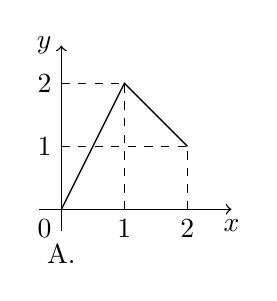
\begin{tikzpicture}[scale=0.8,line width=0.5pt]
\draw[->] (-0.35,0)--(2.7,0) node[below]{$x$};
\draw[->] (0,-0.35)--(0,2.6) node[left]{$y$};
\draw[dashed] (0,1)--(2,1) (0,2)--(1,2) (1,0)--(1,2) (2,0)--(2,1);
\draw (0,0)--(1,2)--(2,1);
\node[below left] at (0,0) {$0$};
\node[below] at (1,0) {$1$}; \node[below] at (2,0) {$2$};
\node[left] at (0,1) {$1$}; \node[left] at (0,2) {$2$};
\node[anchor=north] at (0,-0.4) {A.};
\end{tikzpicture}
&
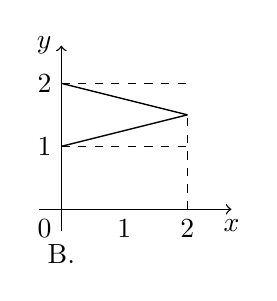
\begin{tikzpicture}[scale=0.8,line width=0.5pt]
\draw[->] (-0.35,0)--(2.7,0) node[below]{$x$};
\draw[->] (0,-0.35)--(0,2.6) node[left]{$y$};
\draw[dashed] (0,1)--(2,1) (0,2)--(2,2) (2,0)--(2,1.5);
\draw (0,2)--(2,1.5);
\draw (0,1)--(2,1.5);
\node[below left] at (0,0) {$0$};
\node[below] at (1,0) {$1$}; \node[below] at (2,0) {$2$};
\node[left] at (0,1) {$1$}; \node[left] at (0,2) {$2$};
\node[anchor=north] at (0,-0.4) {B.};
\end{tikzpicture}
\\[12pt]
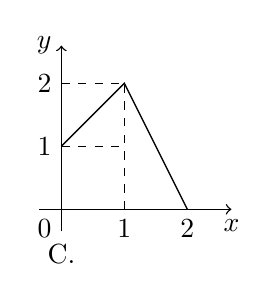
\begin{tikzpicture}[scale=0.8,line width=0.5pt]
\draw[->] (-0.35,0)--(2.7,0) node[below]{$x$};
\draw[->] (0,-0.35)--(0,2.6) node[left]{$y$};
\draw[dashed] (0,1)--(1,1) (0,2)--(1,2) (1,0)--(1,2);
\draw (0,1)--(1,2)--(2,0);
\node[below left] at (0,0) {$0$};
\node[below] at (1,0) {$1$}; \node[below] at (2,0) {$2$};
\node[left] at (0,1) {$1$}; \node[left] at (0,2) {$2$};
\node[anchor=north] at (0,-0.4) {C.};
\end{tikzpicture}
&
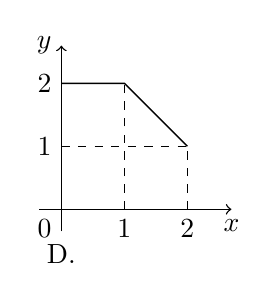
\begin{tikzpicture}[scale=0.8,line width=0.5pt]
\draw[->] (-0.35,0)--(2.7,0) node[below]{$x$};
\draw[->] (0,-0.35)--(0,2.6) node[left]{$y$};
\draw[dashed] (0,1)--(2,1) (1,0)--(1,2) (2,0)--(2,1);
\draw (0,2)--(1,2)--(2,1);
\node[below left] at (0,0) {$0$};
\node[below] at (1,0) {$1$}; \node[below] at (2,0) {$2$};
\node[left] at (0,1) {$1$}; \node[left] at (0,2) {$2$};
\node[anchor=north] at (0,-0.4) {D.};
\end{tikzpicture}
\end{tabular}
\end{center}

\ifanswer
\solbegin
\step{对于 $A$，当 $0\leqslant x\leqslant2$ 时，$0\leqslant y\leqslant2$，故 $A$ 错误；}
\step{对于 $B$，当 $0\leqslant x\leqslant2$ 时，任取一个 $x$ 的值，有两个 $y$ 与之对应，故 $B$ 错误；}
\step{对于 $C$，当 $0\leqslant x\leqslant2$ 时，$0\leqslant y\leqslant2$，故 $C$ 错误；}
\step{对于 $D$，当 $0\leqslant x\leqslant2$ 时，$0\leqslant y\leqslant2$，故 $D$ 正确.}
\step{故选 $D$.}
\solend
\fi

\item 下列函数中与函数 $y=x$ 是同一函数的是\mbox{（\quad）}

\keepwithprev
A. $y=\sqrt{x^2}$\qquad\quad B. $y=(\sqrt x)^2$\qquad\quad C. $u=\dfrac{v^2}{v}$\qquad\quad D. $m=\sqrt[5]{n^5}$

\ifanswer
\solbegin
\step{对于 $A$，$y=\sqrt{x^2}=\lvert x\rvert$，与函数 $y=x$ 的对应关系不相同，不是同一函数；}
\step{对于 $B$，$y=(\sqrt x)^2=x(x\geqslant0)$，与函数 $y=x(x\in\R)$ 的定义域不相同，不是同一函数；}
\step{对于 $C$，$u=\dfrac{v^2}{v}=v(v\neq0)$，与函数 $y=x(x\in\R)$ 的定义域不相同，不是同一函数；}
\step{对于 $D$，$m=\sqrt[5]{n^5}=n(n\in\R)$，与函数 $y=x(x\in\R)$ 的定义域相同，对应关系也相同，是同一函数.}
\step{故选 $D$.}
\solend
\fi

\item 某校高一四班学生 $46$ 人，寒假参加体育训练，其中足球队 $25$ 人，排球队 $22$ 人，游泳队 $24$ 人，足球排球都参加的有 $12$ 人，足球游泳都参加的有 $9$ 人，排球游泳都参加的有 $8$ 人，问：三项都参加的学生数为\mbox{（\quad）}

\keepwithprev
A. $2$\qquad\qquad B. $3$\qquad\qquad C. $4$\qquad\qquad D. $5$

\ifanswer
\solbegin
\step{设集合 $A=\{$参加足球队的学生$\}$，集合 $B=\{$参加排球队的学生$\}$，}
\step{集合 $C=\{$参加游泳队的学生$\}$，}
\step{则 $\operatorname{card}(A)=25$，$\operatorname{card}(B)=22$，$\operatorname{card}(C)=24$，}
\step{$\operatorname{card}(A\cap B)=12$，$\operatorname{card}(A\cap C)=9$，$\operatorname{card}(B\cap C)=8$，}
\step{设三项都参加的有 $x$ 人，即 $\operatorname{card}(A\cap B\cap C)=x$，$\operatorname{card}(A\cup B\cup C)=46$，}
\step{由 $\operatorname{card}(A\cup B\cup C)=\operatorname{card}A+\operatorname{card}B+\operatorname{card}C-\operatorname{card}(A\cap B)$}
\step{$-\operatorname{card}(B\cap C)-\operatorname{card}(A\cap C)+\operatorname{card}(A\cap B\cap C)$，}
\step{即 $46=25+22+24-12-8-9+x$，解得 $x=4$，所以三项都参加的有 $4$ 人.}
\step{故选 $C$.}
\solend
\fi

\item 已知 $\lg a$、$\lg b$ 是方程 $6x^2-4x-3=0$ 的两根，则 $\left(\lg\dfrac ab\right)^2$ 等于\mbox{（\quad）}

\keepwithprev
A. $\dfrac49$\qquad\qquad B. $\dfrac{13}{9}$\qquad\qquad C. $\dfrac{14}{9}$\qquad\qquad D. $\dfrac{22}{9}$

\ifanswer
\solbegin
\step{由韦达定理得 $\lg a+\lg b=\dfrac23$，$\lg a\cdot\lg b=-\dfrac12$，}
\step{所以 $\left(\lg\dfrac ab\right)^2=(\lg a-\lg b)^2=(\lg a+\lg b)^2-4\lg a\lg b=\dfrac49+2=\dfrac{22}{9}$. 故选 $D$.}
\solend
\fi

\end{enumerate}

\bigsec{三、解答题}

\begin{enumerate}
\setcounter{enumi}{16}

\item （1）用分数指数幂表示 $\sqrt[3]{a^2}\cdot\sqrt{a^3}$；

（2）已知 $a^{\frac12}+a^{-\frac12}=3$，求 $a+a^{-1}$.

\ifanswer
\solbegin
\step{（1）$\sqrt[3]{a^2}\cdot\sqrt{a^3}=a^{\frac23}\times a^{\frac32}=a^{\frac{13}6}$.}
\step{（2）由 $a^{\frac12}+a^{-\frac12}=3$，平方得 $a+2+a^{-1}=9$，故 $a+a^{-1}=7$.}
\solend
\fi

\item 已知 $f(x)=\begin{cases}x,x>0\\-x^2-2x+1,x\leqslant0\end{cases}$.

（1）求 $f(f(-2))$ 的值；

（2）若 $f(x_0)=2$，求 $x_0$ 的值.

\ifanswer
\solbegin
\step{（1）$f(x)=\begin{cases}x,x>0\\-x^2-2x+1,x\leqslant0\end{cases}$，则 $f(-2)=-(-2)^2-2\times(-2)+1=1$，}
\step{则有 $f(f(-2))=f(1)=1$；}
\step{（2）当 $x_0>0$ 时，$f(x_0)=x_0$，又 $f(x_0)=2$，所以 $x_0=2$，}
\step{当 $x_0\leqslant0$ 时，$f(x_0)=-x_0^2-2x_0+1$，又 $f(x_0)=2$，}
\step{所以 $-x_0^2-2x_0+1=2$，故 $x_0=-1$，}
\step{综上，$x_0$ 的值为 $-1$ 或 $2$.}
\solend
\fi

\item 已知集合 $A=\{x\mid\lvert 1+x\rvert+\lvert x\rvert<5\}$，$B=\left\{x\,\middle\vert\,\dfrac2{x-m}\geqslant1\right\}$，$p:x\in A$，$q:x\in B$.

（1）若 $m=0$，且 $p$ 真 $q$ 假，求实数 $x$ 的取值范围；

（2）若 $q$ 是 $p$ 的充分不必要条件，求实数 $m$ 的取值范围.

\ifanswer
\solbegin
\step{（1）当 $x\geqslant0$ 时，不等式 $\lvert 1+x\rvert+\lvert x\rvert<5$ 化为 $1+x+x<5$，解得 $0\leqslant x<2$；}
\step{当 $-1\leqslant x<0$ 时，不等式 $\lvert 1+x\rvert+\lvert x\rvert<5$ 化为 $1+x-x<5$ 恒成立，}
\step{故 $-1\leqslant x<0$；}
\step{当 $x<-1$ 时，不等式 $\lvert 1+x\rvert+\lvert x\rvert<5$ 化为 $-1-x-x<5$，}
\step{解得 $-3<x<-1$.}
\step{综上所述，$\lvert 1+x\rvert+\lvert x\rvert<5$ 等价于 $-3<x<2$，}
\step{所以 $\lvert 1+x\rvert+\lvert x\rvert<5$ 的解集为 $A=(-3,2)$，}
\step{若 $m=0$，则 $B=\left\{x\,\middle\vert\,\dfrac2x\geqslant1\right\}=\{x\mid 0<x\leqslant2\}$，得 $\overline{B}=(-\infty,0]\cup(2,+\infty)$，}
\step{由 $p$ 真 $q$ 假，得 $x\in(A\cap\overline{B})=(-3,0]$，即 $x$ 的取值范围为 $(-3,0]$；}
\step{（2）由 $\dfrac2{x-m}\geqslant1$，得 $\begin{cases}x-m>0\\x-m\leqslant2\end{cases}$，解得 $m<x\leqslant m+2$，}
\step{所以 $B=\left\{x\,\middle\vert\,\dfrac2{x-m}\geqslant1\right\}=(m,m+2]$，}
\step{由（1）的结论，得 $A=(-3,2)$，}
\step{若 $q$ 是 $p$ 的充分不必要条件，则 $B$ 是 $A$ 的真子集，得 $\begin{cases}m\geqslant-3\\m+2<2\end{cases}$，}
\step{解得 $-3\leqslant m<0$，即实数 $m$ 的取值范围是 $[-3,0)$.}
\solend
\fi

\item 某企业计划在 $2026$ 年布局人工智能大模型应用开发，生产智能终端配套的 $AI$ 算法服务包. 通过市场分析，全年需投入固定成本 $260$ 万元（含研发、服务器部署等），每生产 $x$ 千个算法服务包，需另投入成本 $R(x)$ 万元，且
$R(x)=\begin{cases}10x^2+100x,0<x\leqslant40\\601x+\dfrac{10000}{x}-7260,x>40\end{cases}$. 已知每个算法服务包的售价为 $0.6$ 万元，假设年内生产的服务包当年能全部销售完.

（1）试写出 $2026$ 年利润 $L$（万元）关于年产量 $x$（千个）的函数解析式；

（2）当 $2026$ 年产量为多少千个时，企业所获利润最大？并求出最大利润.

\ifanswer
\solbegin
\step{（1）$L(x)=x\cdot1000\times0.6-R(x)-260=600x-R(x)-260$，}
\step{当 $0<x\leqslant40$ 时，}
\step{$L(x)=600x-(10x^2+100x)-260=-10x^2+500x-260$；}
\step{当 $x>40$ 时，}
\step{$L(x)=600x-\left(601x+\dfrac{10000}{x}-7260\right)-260=7000-x-\dfrac{10000}{x}$；}
\step{综上，$L(x)=\begin{cases}-10x^2+500x-260,0<x\leqslant40\\7000-x-\dfrac{10000}{x},x>40\end{cases}$；}
\step{（2）当 $0<x\leqslant40$ 时，$L(x)=-10x^2+500x-260=-10(x-25)^2+5990$，}
\step{当 $x=25$ 时，函数 $L(x)$ 有最大值 $5990$；}
\step{当 $x>40$ 时，$L(x)=7000-x-\dfrac{10000}{x}=7000-\left(x+\dfrac{10000}{x}\right)$}
\step{$\leqslant7000-2\sqrt{x\cdot\dfrac{10000}{x}}=7000-2\times100=6800$，}
\step{当且仅当 $x=\dfrac{10000}{x}$ 时取等号，}
\step{所以当 $x=100$ 时，函数 $L(x)$ 有最大值 $6800$；}
\step{因为 $6800>5990$，所以 $2026$ 年产量为 $100$ 千个时，企业所获利润最大，}
\step{最大利润为 $6800$ 万元.}
\solend
\fi

\item 已知二次函数 $f(x)=ax^2+bx+c$.

（1）若 $f(x)>0$ 的解集为 $\{x\mid-3<x<4\}$，解关于 $x$ 的不等式 $bx^2+2ax-(c+3b)<0$；

（2）若函数满足 $f(x+1)-f(x)=2x+2$，且 $f(0)=1$. 求 $f(x)$ 的解析式；

（3）若对任意 $x\in\R$，不等式 $f(x)\geqslant2ax+b$ 恒成立，求 $\dfrac{b^2}{4(a^2+c^2)}$ 的最大值.

\ifanswer
\solbegin
\step{（1）由题意二次函数 $f(x)=ax^2+bx+c$，}
\step{若 $f(x)>0$ 的解集为 $\{x\mid-3<x<4\}$，}
\step{得 $-3$、$4$ 为方程 $ax^2+bx+c=0$ 的根，且 $a<0$，}
\step{则 $\begin{cases}-3+4=-\dfrac ba\\-3\times4=\dfrac ca\end{cases}$，即 $b=-a$，$c=-12a$，}
\step{则不等式 $bx^2+2ax-(c+3b)<0$，即为 $-ax^2+2ax+15a<0(a<0)$，}
\step{则 $x^2-2x-15<0$，解得 $-3<x<5$，}
\step{所以不等式 $bx^2+2ax-(c+3b)<0$ 的解集为 $(-3,5)$；}
\step{（2）由 $f(x)=ax^2+bx+c(a\neq0)$，}
\step{则 $f(x+1)-f(x)=a(x+1)^2+b(x+1)+c-(ax^2+bx+c)=2ax+a+b$，}
\step{又 $f(x+1)-f(x)=2x+2$，故 $\begin{cases}2a=2\\a+b=2\end{cases}$，解得 $a=1$，$b=1$，}
\step{由 $f(0)=1$，得 $c=1$，所以 $f(x)=x^2+x+1$；}
\step{（3）由题意二次函数 $f(x)=ax^2+bx+c$，}
\step{若对任意 $x\in\R$，不等式 $f(x)\geqslant2ax+b$ 恒成立，}
\step{得对任意 $x\in\R$，$ax^2+bx+c\geqslant2ax+b$ 恒成立，}
\step{整理得 $ax^2+(b-2a)x+c-b\geqslant0$ 恒成立，}
\step{因为 $a$ 不为 $0$，所以 $\begin{cases}a>0\\\Delta=(b-2a)^2-4a(c-b)\leqslant0\end{cases}$，}
\step{所以 $0\leqslant b^2\leqslant4a(c-a)$，所以 $\dfrac{b^2}{4(a^2+c^2)}\leqslant\dfrac{ac-a^2}{a^2+c^2}=\dfrac{\frac ca-1}{1+\left(\frac ca\right)^2}$，}
\step{令 $t=\dfrac ca-1$，因为 $0\leqslant b^2\leqslant4a(c-a)$，所以 $c\geqslant a>0\Rightarrow t\geqslant0$，}
\step{若 $t=0$ 时，此时 $\dfrac{b^2}{4(a^2+c^2)}\leqslant\dfrac{\frac ca-1}{1+\left(\frac ca\right)^2}=0$，}
\step{若 $t>0$ 时，$\dfrac{b^2}{4(a^2+c^2)}\leqslant\dfrac{t}{1+(t+1)^2}=\dfrac{t}{t^2+2t+2}=\dfrac1{t+\frac2t+2}$}
\step{$\leqslant\dfrac1{2\sqrt2+2}=\dfrac{\sqrt2-1}{2}$，}
\step{当且仅当 $t=\dfrac2t$，即 $t=\sqrt2$ 时，即 $c=(1+\sqrt2)a$ 时，上式取等号.}
\step{综上所述，$\dfrac{b^2}{4(a^2+c^2)}$ 的最大值为 $\dfrac{\sqrt2-1}{2}$.}
\solend
\fi

\end{enumerate}

\end{document}
"
% 紧凑版：xelatex "\def\iscompact{1}% 高一117_陆行中学_期中.tex
%   —— 高一上数学“2026-2027 年陆行中学高一上期中”（试卷版/答案版）
% 试卷版：xelatex 高一117_陆行中学_期中.tex
% 答案版：xelatex "\def\isanswer{1}\input{高一117_陆行中学_期中.tex}"
% 紧凑版：xelatex "\def\iscompact{1}\input{高一117_陆行中学_期中.tex}"
%
% 原始材料：微信公众号“魔都数学加油站”文章，作者破晓，2026-11-06 17:58 发布；
% 连载“27学年高一117”，原文标题“27学年高一117——2026-2027年上海市陆行中学高一上期中”；
% 原文链接：https://mp.weixin.qq.com/s/of8iPW26dvDyXWohudT0vw。
% 正文为 10 张 PNG 页（第 1、3、4、8、9、10 页 2560×3620，其余 4762×6735），
% 题目下印有【解析】或【答案】，为讲评版。
% 题目、解析均据原图转录；卷面红色水印及公众号页脚未录入。
%
% 卷首标题：原卷印作“2026-2027 年陆行中学高一上期中”（公众号标题中的“上海市”
% 卷面标题行没有，本稿照卷面），年份区间按全稿惯例排 en dash；原卷未印副标题，本稿按题目内容
% 标为“集合与常用逻辑用语、不等式、函数”（期中卷跨三章，含指数／对数与函数，与 112 同）。
%
% 与原卷的排版差异：
%   ① 原文从第 3 题起，填空题 3—12、选择题 13—16、解答题 17—21，共 19 题，本稿保留原题号；
%   ② 原卷每题下直接印【解析】／【答案】，本稿按全稿惯例置于答案版；第 4、6、8 题只印
%      【答案】，另提 \ans{}；其余选择题答案在解析末句“故选 …”，括号内留空；
%   ③ 原卷未印副标题，本稿按“知识模块”口径补出；
%   ④ 原卷填空横线按全稿惯例排为 \blankline[4.4em]；选择题括号排 \mbox{（\quad）}、
%      选项段前按惯例加 \keepwithprev；解答题不留作答区（原卷为讲评版，与 109—116 同）；
%   ⑤ 原卷 $max$／$min$ 排斜体，按 96 成例改 \max／\min；数集 $R$ 按惯例改 \R。
%
% 判别式字形：第 11 题与第 21 题 (3) 的判别式原卷排 $\Delta$（等腰、右厚），照录 \Delta。
%
% 子集符号：第 5 题的 $B\subseteq A$ 印有下划线，照录 \subseteq。
%
% 第 13 题四个坐标图选项按原图形状用 TikZ 重排（三版都出）；原卷另有第 12 题的
%   $a\odot b$ 自定义运算、第 15 题的 $\operatorname{card}$ 记号，均照录。
%
% 原卷存疑照录：第 12 题解析的 $\min\{\left|x\right|\odot\left|3-x\right|\}$ 一行、
%   第 20 题 $R(x)$ 分段函数与 $L(x)$ 的推导，均按原卷印刷行照录。
%   第 20 题题干开头原卷有一段会议背景引语（非数学信息），本稿从“某企业计划在
%   $2026$ 年布局…”起照录题目主体，全部数据、设问与解析均完整保留。
%
% 行数核对：逐题数 \step/\stepm 条数，合计 106 条（Q3：1；Q4：0；Q5：5；Q6：0；Q7：3；
% Q8：0；Q9：3；Q10：3；Q11：5；Q12：6；Q13：5；Q14：5；Q15：9；Q16：2；Q17：2；
% Q18：6；Q19：14；Q20：14；Q21：23），与原卷印刷行逐题相等（cases／TikZ 图块作一个
% 印刷行计）。第 4、6、8 题只印【答案】，提 \ans{}，不计入 \step 账。
%
\documentclass[a4paper,11pt]{article}
\usepackage{common}

\begin{document}

\examtitlest[3]{2026--2027 年陆行中学高一上期中}{集合与常用逻辑用语、不等式、函数}

\bigsec{一、填空题}

\begin{enumerate}
\setcounter{enumi}{2}

\item 已知 $10^a=2$,$10^b=5$，则 $10^{3a-2b}$ 的值为\blankline[4.4em].

\ifanswer
\solbegin
\step{$10^{3a-2b}=\dfrac{10^{3a}}{10^{2b}}=\dfrac{(10^a)^3}{(10^b)^2}=\dfrac{2^3}{5^2}=\dfrac8{25}$.}
\solend
\fi

\item 已知不等式 $\lvert x+1\rvert+\lvert x-3\rvert\geqslant4$ 恒成立，则取等号时 $x$ 的取值范围是\blankline[4.4em].

\ifanswer
\ans{$[-1,3]$}
\fi

\item 集合 $A=\{1,2,a^2\}$，$B=\{2,a\}$，若 $B\subseteq A$，则 $a$ 的值为\blankline[4.4em].

\ifanswer
\solbegin
\step{因为 $B\subseteq A$，所以 $a=1$ 或 $a=a^2$，}
\step{当 $a=1$ 时，$a^2=1$，不满足元素的互异性，故舍去；}
\step{当 $a=a^2$ 时，解得 $a=1$（舍）或 $a=0$，}
\step{当 $a=0$ 时，$A=\{1,2,0\}$，$B=\{2,0\}$，满足题意.}
\step{综上，$a=0$.}
\solend
\fi

\item 若 $x>\dfrac35$，则 $y=5x+\dfrac1{5x-3}$ 的最小值是\blankline[4.4em].

\ifanswer
\ans{$5$}
\fi

\item 已知 $a>0$，$b>0$，且 $a+b=1$，则 $\dfrac3a+\dfrac1b$ 的最小值是\blankline[4.4em].

\ifanswer
\solbegin
\step{$a>0$，$b>0$，且 $a+b=1$，}
\step{$\dfrac3a+\dfrac1b=\left(\dfrac3a+\dfrac1b\right)(a+b)=\dfrac{3b}{a}+\dfrac ab+4\geqslant2\sqrt3+4$，}
\step{当且仅当 $\dfrac{3b}{a}=\dfrac ab$ 时取等号，所以 $\dfrac3a+\dfrac1b$ 的最小值为 $2\sqrt3+4$.}
\solend
\fi

\item 已知 $\log_2 5=a$，则 $\log_5 10=$\blankline[4.4em]（用含 $a$ 的代数式表示）.

\ifanswer
\ans{$1+\dfrac1a$}
\fi

\item 已知 $p:2<x\leqslant3$，$q:\lvert x-a\rvert<2$，若 $p$ 是 $q$ 的充分不必要条件，则实数 $a$ 的取值范围为\blankline[4.4em].

\ifanswer
\solbegin
\step{由 $\lvert x-a\rvert<2$ 得 $a-2<x<a+2$，即 $p:2<x\leqslant3$，$q:a-2<x<a+2$.}
\step{因为 $p$ 是 $q$ 的充分不必要条件，所以 $\begin{cases}a-2\leqslant2\\a+2>3\end{cases}$，解得 $1<a\leqslant4$，}
\step{所以实数 $a$ 的取值范围为 $(1,4]$.}
\solend
\fi

\item 已知 $a>1$,$b>1$，若 $\log_a b+\log_b a=2$，且 $ab=2$，则 $\log_2(a+b)=$\blankline[4.4em].

\ifanswer
\solbegin
\step{由 $\log_a b+\log_b a=2$,$a>1$,$b>1$，得 $\log_a b+\dfrac1{\log_a b}=2$，}
\step{即 $(\log_a b)^2-2\log_a b+1=0$，则 $(\log_a b-1)^2=0$，即 $\log_a b=1$，则 $a=b$，}
\step{又 $ab=2$，则 $a=b=\sqrt2$，所以 $\log_2(a+b)=\log_2(2\sqrt2)=\log_2 2^{\frac32}=\dfrac32$.}
\solend
\fi

\item 已知函数 $f(x)=\sqrt{2kx^2+kx+\dfrac34}$ 的定义域为实数集 $\R$，则实数 $k$ 的取值范围\blankline[4.4em].

\ifanswer
\solbegin
\step{因为函数 $f(x)=\sqrt{2kx^2+kx+\dfrac34}$ 的定义域为实数集 $\R$，}
\step{所以 $2kx^2+kx+\dfrac34\geqslant0$ 在 $\R$ 上恒成立，}
\step{当 $k=0$ 时，$\dfrac34\geqslant0$，恒成立；}
\step{当 $k\neq0$ 时，则有 $\begin{cases}2k>0\\\Delta=k^2-4\times2k\times\dfrac34\leqslant0\end{cases}$，解得 $0<k\leqslant6$；}
\step{综上，实数 $k$ 的取值范围为 $[0,6]$.}
\solend
\fi

\item 对于两个实数 $a$、$b$，定义运算 $a\odot b$ 如下：若 $a\geqslant b$，则 $a\odot b=a$；若 $a<b$，则 $a\odot b=b$. 若 $x$、$y\in\R$，则 $\lvert x-y\rvert\odot\lvert 3-x\rvert\odot\lvert x+y\rvert$ 的最小值是\blankline[4.4em].

\ifanswer
\solbegin
\step{由题意得 $a\odot b=\max\{a,b\}$，所以 $\lvert a+b\rvert\odot\lvert a-b\rvert=\max\{\lvert a+b\rvert,\lvert a-b\rvert\}$，}
\step{设 $\max\{\lvert a+b\rvert,\lvert a-b\rvert\}=M$，则 $\begin{cases}M\geqslant\lvert a+b\rvert\\M\geqslant\lvert a-b\rvert\end{cases}$，}
\step{所以 $2M\geqslant\lvert a+b\rvert+\lvert a-b\rvert\geqslant2\lvert a\rvert$，则 $\lvert a+b\rvert\odot\lvert a-b\rvert\geqslant\lvert a\rvert$，}
\step{所以 $\min\{\lvert x-y\rvert\odot\lvert 3-x\rvert\odot\lvert x+y\rvert\}=\min\{\lvert x-y\rvert\odot\lvert x+y\rvert\odot\lvert 3-x\rvert\}$}
\step{$=\min\{\lvert x\rvert\odot\lvert 3-x\rvert\}=\min\left\{\dfrac32+x\odot\left\lvert\dfrac32-x\right\rvert\right\}=\dfrac32$，}% 原卷该行写法照录
\step{当且仅当 $x=\dfrac32$，$y=0$ 取等号，故 $\lvert x-y\rvert\odot\lvert 3-x\rvert\odot\lvert x+y\rvert$ 的最小值是 $\dfrac32$.}
\solend
\fi

\end{enumerate}

\bigsec{二、选择题}

\begin{enumerate}
\setcounter{enumi}{12}

\item 设 $A=\{x\mid 0\leqslant x\leqslant2\}$，$B=\{y\mid 1\leqslant y\leqslant2\}$，下列图形能表示从集合 $A$ 到集合 $B$ 的函数图像的是\mbox{（\quad）}

\keepwithprev
\begin{center}
% 原卷四个坐标图选项按原图形状用 TikZ 重排。
\begin{tabular}{c@{\qquad\qquad}c}
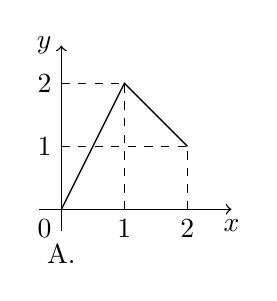
\begin{tikzpicture}[scale=0.8,line width=0.5pt]
\draw[->] (-0.35,0)--(2.7,0) node[below]{$x$};
\draw[->] (0,-0.35)--(0,2.6) node[left]{$y$};
\draw[dashed] (0,1)--(2,1) (0,2)--(1,2) (1,0)--(1,2) (2,0)--(2,1);
\draw (0,0)--(1,2)--(2,1);
\node[below left] at (0,0) {$0$};
\node[below] at (1,0) {$1$}; \node[below] at (2,0) {$2$};
\node[left] at (0,1) {$1$}; \node[left] at (0,2) {$2$};
\node[anchor=north] at (0,-0.4) {A.};
\end{tikzpicture}
&
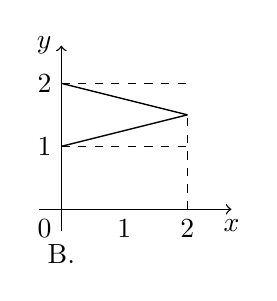
\begin{tikzpicture}[scale=0.8,line width=0.5pt]
\draw[->] (-0.35,0)--(2.7,0) node[below]{$x$};
\draw[->] (0,-0.35)--(0,2.6) node[left]{$y$};
\draw[dashed] (0,1)--(2,1) (0,2)--(2,2) (2,0)--(2,1.5);
\draw (0,2)--(2,1.5);
\draw (0,1)--(2,1.5);
\node[below left] at (0,0) {$0$};
\node[below] at (1,0) {$1$}; \node[below] at (2,0) {$2$};
\node[left] at (0,1) {$1$}; \node[left] at (0,2) {$2$};
\node[anchor=north] at (0,-0.4) {B.};
\end{tikzpicture}
\\[12pt]
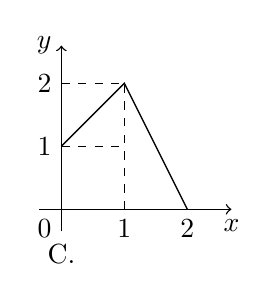
\begin{tikzpicture}[scale=0.8,line width=0.5pt]
\draw[->] (-0.35,0)--(2.7,0) node[below]{$x$};
\draw[->] (0,-0.35)--(0,2.6) node[left]{$y$};
\draw[dashed] (0,1)--(1,1) (0,2)--(1,2) (1,0)--(1,2);
\draw (0,1)--(1,2)--(2,0);
\node[below left] at (0,0) {$0$};
\node[below] at (1,0) {$1$}; \node[below] at (2,0) {$2$};
\node[left] at (0,1) {$1$}; \node[left] at (0,2) {$2$};
\node[anchor=north] at (0,-0.4) {C.};
\end{tikzpicture}
&
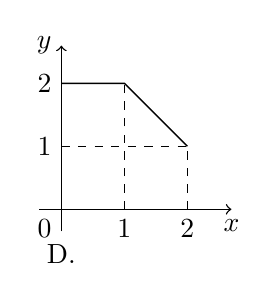
\begin{tikzpicture}[scale=0.8,line width=0.5pt]
\draw[->] (-0.35,0)--(2.7,0) node[below]{$x$};
\draw[->] (0,-0.35)--(0,2.6) node[left]{$y$};
\draw[dashed] (0,1)--(2,1) (1,0)--(1,2) (2,0)--(2,1);
\draw (0,2)--(1,2)--(2,1);
\node[below left] at (0,0) {$0$};
\node[below] at (1,0) {$1$}; \node[below] at (2,0) {$2$};
\node[left] at (0,1) {$1$}; \node[left] at (0,2) {$2$};
\node[anchor=north] at (0,-0.4) {D.};
\end{tikzpicture}
\end{tabular}
\end{center}

\ifanswer
\solbegin
\step{对于 $A$，当 $0\leqslant x\leqslant2$ 时，$0\leqslant y\leqslant2$，故 $A$ 错误；}
\step{对于 $B$，当 $0\leqslant x\leqslant2$ 时，任取一个 $x$ 的值，有两个 $y$ 与之对应，故 $B$ 错误；}
\step{对于 $C$，当 $0\leqslant x\leqslant2$ 时，$0\leqslant y\leqslant2$，故 $C$ 错误；}
\step{对于 $D$，当 $0\leqslant x\leqslant2$ 时，$0\leqslant y\leqslant2$，故 $D$ 正确.}
\step{故选 $D$.}
\solend
\fi

\item 下列函数中与函数 $y=x$ 是同一函数的是\mbox{（\quad）}

\keepwithprev
A. $y=\sqrt{x^2}$\qquad\quad B. $y=(\sqrt x)^2$\qquad\quad C. $u=\dfrac{v^2}{v}$\qquad\quad D. $m=\sqrt[5]{n^5}$

\ifanswer
\solbegin
\step{对于 $A$，$y=\sqrt{x^2}=\lvert x\rvert$，与函数 $y=x$ 的对应关系不相同，不是同一函数；}
\step{对于 $B$，$y=(\sqrt x)^2=x(x\geqslant0)$，与函数 $y=x(x\in\R)$ 的定义域不相同，不是同一函数；}
\step{对于 $C$，$u=\dfrac{v^2}{v}=v(v\neq0)$，与函数 $y=x(x\in\R)$ 的定义域不相同，不是同一函数；}
\step{对于 $D$，$m=\sqrt[5]{n^5}=n(n\in\R)$，与函数 $y=x(x\in\R)$ 的定义域相同，对应关系也相同，是同一函数.}
\step{故选 $D$.}
\solend
\fi

\item 某校高一四班学生 $46$ 人，寒假参加体育训练，其中足球队 $25$ 人，排球队 $22$ 人，游泳队 $24$ 人，足球排球都参加的有 $12$ 人，足球游泳都参加的有 $9$ 人，排球游泳都参加的有 $8$ 人，问：三项都参加的学生数为\mbox{（\quad）}

\keepwithprev
A. $2$\qquad\qquad B. $3$\qquad\qquad C. $4$\qquad\qquad D. $5$

\ifanswer
\solbegin
\step{设集合 $A=\{$参加足球队的学生$\}$，集合 $B=\{$参加排球队的学生$\}$，}
\step{集合 $C=\{$参加游泳队的学生$\}$，}
\step{则 $\operatorname{card}(A)=25$，$\operatorname{card}(B)=22$，$\operatorname{card}(C)=24$，}
\step{$\operatorname{card}(A\cap B)=12$，$\operatorname{card}(A\cap C)=9$，$\operatorname{card}(B\cap C)=8$，}
\step{设三项都参加的有 $x$ 人，即 $\operatorname{card}(A\cap B\cap C)=x$，$\operatorname{card}(A\cup B\cup C)=46$，}
\step{由 $\operatorname{card}(A\cup B\cup C)=\operatorname{card}A+\operatorname{card}B+\operatorname{card}C-\operatorname{card}(A\cap B)$}
\step{$-\operatorname{card}(B\cap C)-\operatorname{card}(A\cap C)+\operatorname{card}(A\cap B\cap C)$，}
\step{即 $46=25+22+24-12-8-9+x$，解得 $x=4$，所以三项都参加的有 $4$ 人.}
\step{故选 $C$.}
\solend
\fi

\item 已知 $\lg a$、$\lg b$ 是方程 $6x^2-4x-3=0$ 的两根，则 $\left(\lg\dfrac ab\right)^2$ 等于\mbox{（\quad）}

\keepwithprev
A. $\dfrac49$\qquad\qquad B. $\dfrac{13}{9}$\qquad\qquad C. $\dfrac{14}{9}$\qquad\qquad D. $\dfrac{22}{9}$

\ifanswer
\solbegin
\step{由韦达定理得 $\lg a+\lg b=\dfrac23$，$\lg a\cdot\lg b=-\dfrac12$，}
\step{所以 $\left(\lg\dfrac ab\right)^2=(\lg a-\lg b)^2=(\lg a+\lg b)^2-4\lg a\lg b=\dfrac49+2=\dfrac{22}{9}$. 故选 $D$.}
\solend
\fi

\end{enumerate}

\bigsec{三、解答题}

\begin{enumerate}
\setcounter{enumi}{16}

\item （1）用分数指数幂表示 $\sqrt[3]{a^2}\cdot\sqrt{a^3}$；

（2）已知 $a^{\frac12}+a^{-\frac12}=3$，求 $a+a^{-1}$.

\ifanswer
\solbegin
\step{（1）$\sqrt[3]{a^2}\cdot\sqrt{a^3}=a^{\frac23}\times a^{\frac32}=a^{\frac{13}6}$.}
\step{（2）由 $a^{\frac12}+a^{-\frac12}=3$，平方得 $a+2+a^{-1}=9$，故 $a+a^{-1}=7$.}
\solend
\fi

\item 已知 $f(x)=\begin{cases}x,x>0\\-x^2-2x+1,x\leqslant0\end{cases}$.

（1）求 $f(f(-2))$ 的值；

（2）若 $f(x_0)=2$，求 $x_0$ 的值.

\ifanswer
\solbegin
\step{（1）$f(x)=\begin{cases}x,x>0\\-x^2-2x+1,x\leqslant0\end{cases}$，则 $f(-2)=-(-2)^2-2\times(-2)+1=1$，}
\step{则有 $f(f(-2))=f(1)=1$；}
\step{（2）当 $x_0>0$ 时，$f(x_0)=x_0$，又 $f(x_0)=2$，所以 $x_0=2$，}
\step{当 $x_0\leqslant0$ 时，$f(x_0)=-x_0^2-2x_0+1$，又 $f(x_0)=2$，}
\step{所以 $-x_0^2-2x_0+1=2$，故 $x_0=-1$，}
\step{综上，$x_0$ 的值为 $-1$ 或 $2$.}
\solend
\fi

\item 已知集合 $A=\{x\mid\lvert 1+x\rvert+\lvert x\rvert<5\}$，$B=\left\{x\,\middle\vert\,\dfrac2{x-m}\geqslant1\right\}$，$p:x\in A$，$q:x\in B$.

（1）若 $m=0$，且 $p$ 真 $q$ 假，求实数 $x$ 的取值范围；

（2）若 $q$ 是 $p$ 的充分不必要条件，求实数 $m$ 的取值范围.

\ifanswer
\solbegin
\step{（1）当 $x\geqslant0$ 时，不等式 $\lvert 1+x\rvert+\lvert x\rvert<5$ 化为 $1+x+x<5$，解得 $0\leqslant x<2$；}
\step{当 $-1\leqslant x<0$ 时，不等式 $\lvert 1+x\rvert+\lvert x\rvert<5$ 化为 $1+x-x<5$ 恒成立，}
\step{故 $-1\leqslant x<0$；}
\step{当 $x<-1$ 时，不等式 $\lvert 1+x\rvert+\lvert x\rvert<5$ 化为 $-1-x-x<5$，}
\step{解得 $-3<x<-1$.}
\step{综上所述，$\lvert 1+x\rvert+\lvert x\rvert<5$ 等价于 $-3<x<2$，}
\step{所以 $\lvert 1+x\rvert+\lvert x\rvert<5$ 的解集为 $A=(-3,2)$，}
\step{若 $m=0$，则 $B=\left\{x\,\middle\vert\,\dfrac2x\geqslant1\right\}=\{x\mid 0<x\leqslant2\}$，得 $\overline{B}=(-\infty,0]\cup(2,+\infty)$，}
\step{由 $p$ 真 $q$ 假，得 $x\in(A\cap\overline{B})=(-3,0]$，即 $x$ 的取值范围为 $(-3,0]$；}
\step{（2）由 $\dfrac2{x-m}\geqslant1$，得 $\begin{cases}x-m>0\\x-m\leqslant2\end{cases}$，解得 $m<x\leqslant m+2$，}
\step{所以 $B=\left\{x\,\middle\vert\,\dfrac2{x-m}\geqslant1\right\}=(m,m+2]$，}
\step{由（1）的结论，得 $A=(-3,2)$，}
\step{若 $q$ 是 $p$ 的充分不必要条件，则 $B$ 是 $A$ 的真子集，得 $\begin{cases}m\geqslant-3\\m+2<2\end{cases}$，}
\step{解得 $-3\leqslant m<0$，即实数 $m$ 的取值范围是 $[-3,0)$.}
\solend
\fi

\item 某企业计划在 $2026$ 年布局人工智能大模型应用开发，生产智能终端配套的 $AI$ 算法服务包. 通过市场分析，全年需投入固定成本 $260$ 万元（含研发、服务器部署等），每生产 $x$ 千个算法服务包，需另投入成本 $R(x)$ 万元，且
$R(x)=\begin{cases}10x^2+100x,0<x\leqslant40\\601x+\dfrac{10000}{x}-7260,x>40\end{cases}$. 已知每个算法服务包的售价为 $0.6$ 万元，假设年内生产的服务包当年能全部销售完.

（1）试写出 $2026$ 年利润 $L$（万元）关于年产量 $x$（千个）的函数解析式；

（2）当 $2026$ 年产量为多少千个时，企业所获利润最大？并求出最大利润.

\ifanswer
\solbegin
\step{（1）$L(x)=x\cdot1000\times0.6-R(x)-260=600x-R(x)-260$，}
\step{当 $0<x\leqslant40$ 时，}
\step{$L(x)=600x-(10x^2+100x)-260=-10x^2+500x-260$；}
\step{当 $x>40$ 时，}
\step{$L(x)=600x-\left(601x+\dfrac{10000}{x}-7260\right)-260=7000-x-\dfrac{10000}{x}$；}
\step{综上，$L(x)=\begin{cases}-10x^2+500x-260,0<x\leqslant40\\7000-x-\dfrac{10000}{x},x>40\end{cases}$；}
\step{（2）当 $0<x\leqslant40$ 时，$L(x)=-10x^2+500x-260=-10(x-25)^2+5990$，}
\step{当 $x=25$ 时，函数 $L(x)$ 有最大值 $5990$；}
\step{当 $x>40$ 时，$L(x)=7000-x-\dfrac{10000}{x}=7000-\left(x+\dfrac{10000}{x}\right)$}
\step{$\leqslant7000-2\sqrt{x\cdot\dfrac{10000}{x}}=7000-2\times100=6800$，}
\step{当且仅当 $x=\dfrac{10000}{x}$ 时取等号，}
\step{所以当 $x=100$ 时，函数 $L(x)$ 有最大值 $6800$；}
\step{因为 $6800>5990$，所以 $2026$ 年产量为 $100$ 千个时，企业所获利润最大，}
\step{最大利润为 $6800$ 万元.}
\solend
\fi

\item 已知二次函数 $f(x)=ax^2+bx+c$.

（1）若 $f(x)>0$ 的解集为 $\{x\mid-3<x<4\}$，解关于 $x$ 的不等式 $bx^2+2ax-(c+3b)<0$；

（2）若函数满足 $f(x+1)-f(x)=2x+2$，且 $f(0)=1$. 求 $f(x)$ 的解析式；

（3）若对任意 $x\in\R$，不等式 $f(x)\geqslant2ax+b$ 恒成立，求 $\dfrac{b^2}{4(a^2+c^2)}$ 的最大值.

\ifanswer
\solbegin
\step{（1）由题意二次函数 $f(x)=ax^2+bx+c$，}
\step{若 $f(x)>0$ 的解集为 $\{x\mid-3<x<4\}$，}
\step{得 $-3$、$4$ 为方程 $ax^2+bx+c=0$ 的根，且 $a<0$，}
\step{则 $\begin{cases}-3+4=-\dfrac ba\\-3\times4=\dfrac ca\end{cases}$，即 $b=-a$，$c=-12a$，}
\step{则不等式 $bx^2+2ax-(c+3b)<0$，即为 $-ax^2+2ax+15a<0(a<0)$，}
\step{则 $x^2-2x-15<0$，解得 $-3<x<5$，}
\step{所以不等式 $bx^2+2ax-(c+3b)<0$ 的解集为 $(-3,5)$；}
\step{（2）由 $f(x)=ax^2+bx+c(a\neq0)$，}
\step{则 $f(x+1)-f(x)=a(x+1)^2+b(x+1)+c-(ax^2+bx+c)=2ax+a+b$，}
\step{又 $f(x+1)-f(x)=2x+2$，故 $\begin{cases}2a=2\\a+b=2\end{cases}$，解得 $a=1$，$b=1$，}
\step{由 $f(0)=1$，得 $c=1$，所以 $f(x)=x^2+x+1$；}
\step{（3）由题意二次函数 $f(x)=ax^2+bx+c$，}
\step{若对任意 $x\in\R$，不等式 $f(x)\geqslant2ax+b$ 恒成立，}
\step{得对任意 $x\in\R$，$ax^2+bx+c\geqslant2ax+b$ 恒成立，}
\step{整理得 $ax^2+(b-2a)x+c-b\geqslant0$ 恒成立，}
\step{因为 $a$ 不为 $0$，所以 $\begin{cases}a>0\\\Delta=(b-2a)^2-4a(c-b)\leqslant0\end{cases}$，}
\step{所以 $0\leqslant b^2\leqslant4a(c-a)$，所以 $\dfrac{b^2}{4(a^2+c^2)}\leqslant\dfrac{ac-a^2}{a^2+c^2}=\dfrac{\frac ca-1}{1+\left(\frac ca\right)^2}$，}
\step{令 $t=\dfrac ca-1$，因为 $0\leqslant b^2\leqslant4a(c-a)$，所以 $c\geqslant a>0\Rightarrow t\geqslant0$，}
\step{若 $t=0$ 时，此时 $\dfrac{b^2}{4(a^2+c^2)}\leqslant\dfrac{\frac ca-1}{1+\left(\frac ca\right)^2}=0$，}
\step{若 $t>0$ 时，$\dfrac{b^2}{4(a^2+c^2)}\leqslant\dfrac{t}{1+(t+1)^2}=\dfrac{t}{t^2+2t+2}=\dfrac1{t+\frac2t+2}$}
\step{$\leqslant\dfrac1{2\sqrt2+2}=\dfrac{\sqrt2-1}{2}$，}
\step{当且仅当 $t=\dfrac2t$，即 $t=\sqrt2$ 时，即 $c=(1+\sqrt2)a$ 时，上式取等号.}
\step{综上所述，$\dfrac{b^2}{4(a^2+c^2)}$ 的最大值为 $\dfrac{\sqrt2-1}{2}$.}
\solend
\fi

\end{enumerate}

\end{document}
"
%
% 原始材料：微信公众号“魔都数学加油站”文章，作者破晓，2026-11-06 17:58 发布；
% 连载“27学年高一117”，原文标题“27学年高一117——2026-2027年上海市陆行中学高一上期中”；
% 原文链接：https://mp.weixin.qq.com/s/of8iPW26dvDyXWohudT0vw。
% 正文为 10 张 PNG 页（第 1、3、4、8、9、10 页 2560×3620，其余 4762×6735），
% 题目下印有【解析】或【答案】，为讲评版。
% 题目、解析均据原图转录；卷面红色水印及公众号页脚未录入。
%
% 卷首标题：原卷印作“2026-2027 年陆行中学高一上期中”（公众号标题中的“上海市”
% 卷面标题行没有，本稿照卷面），年份区间按全稿惯例排 en dash；原卷未印副标题，本稿按题目内容
% 标为“集合与常用逻辑用语、不等式、函数”（期中卷跨三章，含指数／对数与函数，与 112 同）。
%
% 与原卷的排版差异：
%   ① 原文从第 3 题起，填空题 3—12、选择题 13—16、解答题 17—21，共 19 题，本稿保留原题号；
%   ② 原卷每题下直接印【解析】／【答案】，本稿按全稿惯例置于答案版；第 4、6、8 题只印
%      【答案】，另提 \ans{}；其余选择题答案在解析末句“故选 …”，括号内留空；
%   ③ 原卷未印副标题，本稿按“知识模块”口径补出；
%   ④ 原卷填空横线按全稿惯例排为 \blankline[4.4em]；选择题括号排 \mbox{（\quad）}、
%      选项段前按惯例加 \keepwithprev；解答题不留作答区（原卷为讲评版，与 109—116 同）；
%   ⑤ 原卷 $max$／$min$ 排斜体，按 96 成例改 \max／\min；数集 $R$ 按惯例改 \R。
%
% 判别式字形：第 11 题与第 21 题 (3) 的判别式原卷排 $\Delta$（等腰、右厚），照录 \Delta。
%
% 子集符号：第 5 题的 $B\subseteq A$ 印有下划线，照录 \subseteq。
%
% 第 13 题四个坐标图选项按原图形状用 TikZ 重排（三版都出）；原卷另有第 12 题的
%   $a\odot b$ 自定义运算、第 15 题的 $\operatorname{card}$ 记号，均照录。
%
% 原卷存疑照录：第 12 题解析的 $\min\{\left|x\right|\odot\left|3-x\right|\}$ 一行、
%   第 20 题 $R(x)$ 分段函数与 $L(x)$ 的推导，均按原卷印刷行照录。
%   第 20 题题干开头原卷有一段会议背景引语（非数学信息），本稿从“某企业计划在
%   $2026$ 年布局…”起照录题目主体，全部数据、设问与解析均完整保留。
%
% 行数核对：逐题数 \step/\stepm 条数，合计 106 条（Q3：1；Q4：0；Q5：5；Q6：0；Q7：3；
% Q8：0；Q9：3；Q10：3；Q11：5；Q12：6；Q13：5；Q14：5；Q15：9；Q16：2；Q17：2；
% Q18：6；Q19：14；Q20：14；Q21：23），与原卷印刷行逐题相等（cases／TikZ 图块作一个
% 印刷行计）。第 4、6、8 题只印【答案】，提 \ans{}，不计入 \step 账。
%
\documentclass[a4paper,11pt]{article}
\usepackage{common}

\begin{document}

\examtitlest[3]{2026--2027 年陆行中学高一上期中}{集合与常用逻辑用语、不等式、函数}

\bigsec{一、填空题}

\begin{enumerate}
\setcounter{enumi}{2}

\item 已知 $10^a=2$,$10^b=5$，则 $10^{3a-2b}$ 的值为\blankline[4.4em].

\ifanswer
\solbegin
\step{$10^{3a-2b}=\dfrac{10^{3a}}{10^{2b}}=\dfrac{(10^a)^3}{(10^b)^2}=\dfrac{2^3}{5^2}=\dfrac8{25}$.}
\solend
\fi

\item 已知不等式 $\lvert x+1\rvert+\lvert x-3\rvert\geqslant4$ 恒成立，则取等号时 $x$ 的取值范围是\blankline[4.4em].

\ifanswer
\ans{$[-1,3]$}
\fi

\item 集合 $A=\{1,2,a^2\}$，$B=\{2,a\}$，若 $B\subseteq A$，则 $a$ 的值为\blankline[4.4em].

\ifanswer
\solbegin
\step{因为 $B\subseteq A$，所以 $a=1$ 或 $a=a^2$，}
\step{当 $a=1$ 时，$a^2=1$，不满足元素的互异性，故舍去；}
\step{当 $a=a^2$ 时，解得 $a=1$（舍）或 $a=0$，}
\step{当 $a=0$ 时，$A=\{1,2,0\}$，$B=\{2,0\}$，满足题意.}
\step{综上，$a=0$.}
\solend
\fi

\item 若 $x>\dfrac35$，则 $y=5x+\dfrac1{5x-3}$ 的最小值是\blankline[4.4em].

\ifanswer
\ans{$5$}
\fi

\item 已知 $a>0$，$b>0$，且 $a+b=1$，则 $\dfrac3a+\dfrac1b$ 的最小值是\blankline[4.4em].

\ifanswer
\solbegin
\step{$a>0$，$b>0$，且 $a+b=1$，}
\step{$\dfrac3a+\dfrac1b=\left(\dfrac3a+\dfrac1b\right)(a+b)=\dfrac{3b}{a}+\dfrac ab+4\geqslant2\sqrt3+4$，}
\step{当且仅当 $\dfrac{3b}{a}=\dfrac ab$ 时取等号，所以 $\dfrac3a+\dfrac1b$ 的最小值为 $2\sqrt3+4$.}
\solend
\fi

\item 已知 $\log_2 5=a$，则 $\log_5 10=$\blankline[4.4em]（用含 $a$ 的代数式表示）.

\ifanswer
\ans{$1+\dfrac1a$}
\fi

\item 已知 $p:2<x\leqslant3$，$q:\lvert x-a\rvert<2$，若 $p$ 是 $q$ 的充分不必要条件，则实数 $a$ 的取值范围为\blankline[4.4em].

\ifanswer
\solbegin
\step{由 $\lvert x-a\rvert<2$ 得 $a-2<x<a+2$，即 $p:2<x\leqslant3$，$q:a-2<x<a+2$.}
\step{因为 $p$ 是 $q$ 的充分不必要条件，所以 $\begin{cases}a-2\leqslant2\\a+2>3\end{cases}$，解得 $1<a\leqslant4$，}
\step{所以实数 $a$ 的取值范围为 $(1,4]$.}
\solend
\fi

\item 已知 $a>1$,$b>1$，若 $\log_a b+\log_b a=2$，且 $ab=2$，则 $\log_2(a+b)=$\blankline[4.4em].

\ifanswer
\solbegin
\step{由 $\log_a b+\log_b a=2$,$a>1$,$b>1$，得 $\log_a b+\dfrac1{\log_a b}=2$，}
\step{即 $(\log_a b)^2-2\log_a b+1=0$，则 $(\log_a b-1)^2=0$，即 $\log_a b=1$，则 $a=b$，}
\step{又 $ab=2$，则 $a=b=\sqrt2$，所以 $\log_2(a+b)=\log_2(2\sqrt2)=\log_2 2^{\frac32}=\dfrac32$.}
\solend
\fi

\item 已知函数 $f(x)=\sqrt{2kx^2+kx+\dfrac34}$ 的定义域为实数集 $\R$，则实数 $k$ 的取值范围\blankline[4.4em].

\ifanswer
\solbegin
\step{因为函数 $f(x)=\sqrt{2kx^2+kx+\dfrac34}$ 的定义域为实数集 $\R$，}
\step{所以 $2kx^2+kx+\dfrac34\geqslant0$ 在 $\R$ 上恒成立，}
\step{当 $k=0$ 时，$\dfrac34\geqslant0$，恒成立；}
\step{当 $k\neq0$ 时，则有 $\begin{cases}2k>0\\\Delta=k^2-4\times2k\times\dfrac34\leqslant0\end{cases}$，解得 $0<k\leqslant6$；}
\step{综上，实数 $k$ 的取值范围为 $[0,6]$.}
\solend
\fi

\item 对于两个实数 $a$、$b$，定义运算 $a\odot b$ 如下：若 $a\geqslant b$，则 $a\odot b=a$；若 $a<b$，则 $a\odot b=b$. 若 $x$、$y\in\R$，则 $\lvert x-y\rvert\odot\lvert 3-x\rvert\odot\lvert x+y\rvert$ 的最小值是\blankline[4.4em].

\ifanswer
\solbegin
\step{由题意得 $a\odot b=\max\{a,b\}$，所以 $\lvert a+b\rvert\odot\lvert a-b\rvert=\max\{\lvert a+b\rvert,\lvert a-b\rvert\}$，}
\step{设 $\max\{\lvert a+b\rvert,\lvert a-b\rvert\}=M$，则 $\begin{cases}M\geqslant\lvert a+b\rvert\\M\geqslant\lvert a-b\rvert\end{cases}$，}
\step{所以 $2M\geqslant\lvert a+b\rvert+\lvert a-b\rvert\geqslant2\lvert a\rvert$，则 $\lvert a+b\rvert\odot\lvert a-b\rvert\geqslant\lvert a\rvert$，}
\step{所以 $\min\{\lvert x-y\rvert\odot\lvert 3-x\rvert\odot\lvert x+y\rvert\}=\min\{\lvert x-y\rvert\odot\lvert x+y\rvert\odot\lvert 3-x\rvert\}$}
\step{$=\min\{\lvert x\rvert\odot\lvert 3-x\rvert\}=\min\left\{\dfrac32+x\odot\left\lvert\dfrac32-x\right\rvert\right\}=\dfrac32$，}% 原卷该行写法照录
\step{当且仅当 $x=\dfrac32$，$y=0$ 取等号，故 $\lvert x-y\rvert\odot\lvert 3-x\rvert\odot\lvert x+y\rvert$ 的最小值是 $\dfrac32$.}
\solend
\fi

\end{enumerate}

\bigsec{二、选择题}

\begin{enumerate}
\setcounter{enumi}{12}

\item 设 $A=\{x\mid 0\leqslant x\leqslant2\}$，$B=\{y\mid 1\leqslant y\leqslant2\}$，下列图形能表示从集合 $A$ 到集合 $B$ 的函数图像的是\mbox{（\quad）}

\keepwithprev
\begin{center}
% 原卷四个坐标图选项按原图形状用 TikZ 重排。
\begin{tabular}{c@{\qquad\qquad}c}
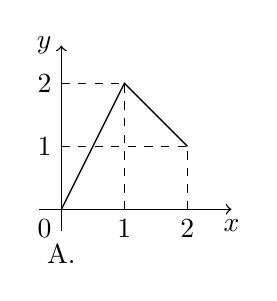
\begin{tikzpicture}[scale=0.8,line width=0.5pt]
\draw[->] (-0.35,0)--(2.7,0) node[below]{$x$};
\draw[->] (0,-0.35)--(0,2.6) node[left]{$y$};
\draw[dashed] (0,1)--(2,1) (0,2)--(1,2) (1,0)--(1,2) (2,0)--(2,1);
\draw (0,0)--(1,2)--(2,1);
\node[below left] at (0,0) {$0$};
\node[below] at (1,0) {$1$}; \node[below] at (2,0) {$2$};
\node[left] at (0,1) {$1$}; \node[left] at (0,2) {$2$};
\node[anchor=north] at (0,-0.4) {A.};
\end{tikzpicture}
&
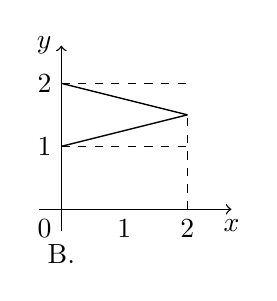
\begin{tikzpicture}[scale=0.8,line width=0.5pt]
\draw[->] (-0.35,0)--(2.7,0) node[below]{$x$};
\draw[->] (0,-0.35)--(0,2.6) node[left]{$y$};
\draw[dashed] (0,1)--(2,1) (0,2)--(2,2) (2,0)--(2,1.5);
\draw (0,2)--(2,1.5);
\draw (0,1)--(2,1.5);
\node[below left] at (0,0) {$0$};
\node[below] at (1,0) {$1$}; \node[below] at (2,0) {$2$};
\node[left] at (0,1) {$1$}; \node[left] at (0,2) {$2$};
\node[anchor=north] at (0,-0.4) {B.};
\end{tikzpicture}
\\[12pt]
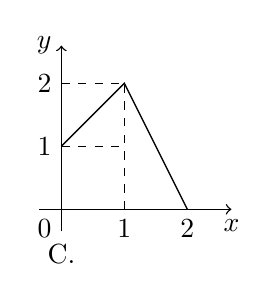
\begin{tikzpicture}[scale=0.8,line width=0.5pt]
\draw[->] (-0.35,0)--(2.7,0) node[below]{$x$};
\draw[->] (0,-0.35)--(0,2.6) node[left]{$y$};
\draw[dashed] (0,1)--(1,1) (0,2)--(1,2) (1,0)--(1,2);
\draw (0,1)--(1,2)--(2,0);
\node[below left] at (0,0) {$0$};
\node[below] at (1,0) {$1$}; \node[below] at (2,0) {$2$};
\node[left] at (0,1) {$1$}; \node[left] at (0,2) {$2$};
\node[anchor=north] at (0,-0.4) {C.};
\end{tikzpicture}
&
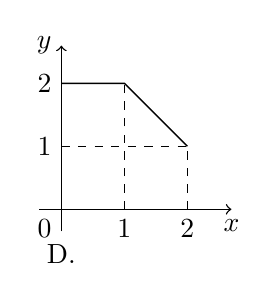
\begin{tikzpicture}[scale=0.8,line width=0.5pt]
\draw[->] (-0.35,0)--(2.7,0) node[below]{$x$};
\draw[->] (0,-0.35)--(0,2.6) node[left]{$y$};
\draw[dashed] (0,1)--(2,1) (1,0)--(1,2) (2,0)--(2,1);
\draw (0,2)--(1,2)--(2,1);
\node[below left] at (0,0) {$0$};
\node[below] at (1,0) {$1$}; \node[below] at (2,0) {$2$};
\node[left] at (0,1) {$1$}; \node[left] at (0,2) {$2$};
\node[anchor=north] at (0,-0.4) {D.};
\end{tikzpicture}
\end{tabular}
\end{center}

\ifanswer
\solbegin
\step{对于 $A$，当 $0\leqslant x\leqslant2$ 时，$0\leqslant y\leqslant2$，故 $A$ 错误；}
\step{对于 $B$，当 $0\leqslant x\leqslant2$ 时，任取一个 $x$ 的值，有两个 $y$ 与之对应，故 $B$ 错误；}
\step{对于 $C$，当 $0\leqslant x\leqslant2$ 时，$0\leqslant y\leqslant2$，故 $C$ 错误；}
\step{对于 $D$，当 $0\leqslant x\leqslant2$ 时，$0\leqslant y\leqslant2$，故 $D$ 正确.}
\step{故选 $D$.}
\solend
\fi

\item 下列函数中与函数 $y=x$ 是同一函数的是\mbox{（\quad）}

\keepwithprev
A. $y=\sqrt{x^2}$\qquad\quad B. $y=(\sqrt x)^2$\qquad\quad C. $u=\dfrac{v^2}{v}$\qquad\quad D. $m=\sqrt[5]{n^5}$

\ifanswer
\solbegin
\step{对于 $A$，$y=\sqrt{x^2}=\lvert x\rvert$，与函数 $y=x$ 的对应关系不相同，不是同一函数；}
\step{对于 $B$，$y=(\sqrt x)^2=x(x\geqslant0)$，与函数 $y=x(x\in\R)$ 的定义域不相同，不是同一函数；}
\step{对于 $C$，$u=\dfrac{v^2}{v}=v(v\neq0)$，与函数 $y=x(x\in\R)$ 的定义域不相同，不是同一函数；}
\step{对于 $D$，$m=\sqrt[5]{n^5}=n(n\in\R)$，与函数 $y=x(x\in\R)$ 的定义域相同，对应关系也相同，是同一函数.}
\step{故选 $D$.}
\solend
\fi

\item 某校高一四班学生 $46$ 人，寒假参加体育训练，其中足球队 $25$ 人，排球队 $22$ 人，游泳队 $24$ 人，足球排球都参加的有 $12$ 人，足球游泳都参加的有 $9$ 人，排球游泳都参加的有 $8$ 人，问：三项都参加的学生数为\mbox{（\quad）}

\keepwithprev
A. $2$\qquad\qquad B. $3$\qquad\qquad C. $4$\qquad\qquad D. $5$

\ifanswer
\solbegin
\step{设集合 $A=\{$参加足球队的学生$\}$，集合 $B=\{$参加排球队的学生$\}$，}
\step{集合 $C=\{$参加游泳队的学生$\}$，}
\step{则 $\operatorname{card}(A)=25$，$\operatorname{card}(B)=22$，$\operatorname{card}(C)=24$，}
\step{$\operatorname{card}(A\cap B)=12$，$\operatorname{card}(A\cap C)=9$，$\operatorname{card}(B\cap C)=8$，}
\step{设三项都参加的有 $x$ 人，即 $\operatorname{card}(A\cap B\cap C)=x$，$\operatorname{card}(A\cup B\cup C)=46$，}
\step{由 $\operatorname{card}(A\cup B\cup C)=\operatorname{card}A+\operatorname{card}B+\operatorname{card}C-\operatorname{card}(A\cap B)$}
\step{$-\operatorname{card}(B\cap C)-\operatorname{card}(A\cap C)+\operatorname{card}(A\cap B\cap C)$，}
\step{即 $46=25+22+24-12-8-9+x$，解得 $x=4$，所以三项都参加的有 $4$ 人.}
\step{故选 $C$.}
\solend
\fi

\item 已知 $\lg a$、$\lg b$ 是方程 $6x^2-4x-3=0$ 的两根，则 $\left(\lg\dfrac ab\right)^2$ 等于\mbox{（\quad）}

\keepwithprev
A. $\dfrac49$\qquad\qquad B. $\dfrac{13}{9}$\qquad\qquad C. $\dfrac{14}{9}$\qquad\qquad D. $\dfrac{22}{9}$

\ifanswer
\solbegin
\step{由韦达定理得 $\lg a+\lg b=\dfrac23$，$\lg a\cdot\lg b=-\dfrac12$，}
\step{所以 $\left(\lg\dfrac ab\right)^2=(\lg a-\lg b)^2=(\lg a+\lg b)^2-4\lg a\lg b=\dfrac49+2=\dfrac{22}{9}$. 故选 $D$.}
\solend
\fi

\end{enumerate}

\bigsec{三、解答题}

\begin{enumerate}
\setcounter{enumi}{16}

\item （1）用分数指数幂表示 $\sqrt[3]{a^2}\cdot\sqrt{a^3}$；

（2）已知 $a^{\frac12}+a^{-\frac12}=3$，求 $a+a^{-1}$.

\ifanswer
\solbegin
\step{（1）$\sqrt[3]{a^2}\cdot\sqrt{a^3}=a^{\frac23}\times a^{\frac32}=a^{\frac{13}6}$.}
\step{（2）由 $a^{\frac12}+a^{-\frac12}=3$，平方得 $a+2+a^{-1}=9$，故 $a+a^{-1}=7$.}
\solend
\fi

\item 已知 $f(x)=\begin{cases}x,x>0\\-x^2-2x+1,x\leqslant0\end{cases}$.

（1）求 $f(f(-2))$ 的值；

（2）若 $f(x_0)=2$，求 $x_0$ 的值.

\ifanswer
\solbegin
\step{（1）$f(x)=\begin{cases}x,x>0\\-x^2-2x+1,x\leqslant0\end{cases}$，则 $f(-2)=-(-2)^2-2\times(-2)+1=1$，}
\step{则有 $f(f(-2))=f(1)=1$；}
\step{（2）当 $x_0>0$ 时，$f(x_0)=x_0$，又 $f(x_0)=2$，所以 $x_0=2$，}
\step{当 $x_0\leqslant0$ 时，$f(x_0)=-x_0^2-2x_0+1$，又 $f(x_0)=2$，}
\step{所以 $-x_0^2-2x_0+1=2$，故 $x_0=-1$，}
\step{综上，$x_0$ 的值为 $-1$ 或 $2$.}
\solend
\fi

\item 已知集合 $A=\{x\mid\lvert 1+x\rvert+\lvert x\rvert<5\}$，$B=\left\{x\,\middle\vert\,\dfrac2{x-m}\geqslant1\right\}$，$p:x\in A$，$q:x\in B$.

（1）若 $m=0$，且 $p$ 真 $q$ 假，求实数 $x$ 的取值范围；

（2）若 $q$ 是 $p$ 的充分不必要条件，求实数 $m$ 的取值范围.

\ifanswer
\solbegin
\step{（1）当 $x\geqslant0$ 时，不等式 $\lvert 1+x\rvert+\lvert x\rvert<5$ 化为 $1+x+x<5$，解得 $0\leqslant x<2$；}
\step{当 $-1\leqslant x<0$ 时，不等式 $\lvert 1+x\rvert+\lvert x\rvert<5$ 化为 $1+x-x<5$ 恒成立，}
\step{故 $-1\leqslant x<0$；}
\step{当 $x<-1$ 时，不等式 $\lvert 1+x\rvert+\lvert x\rvert<5$ 化为 $-1-x-x<5$，}
\step{解得 $-3<x<-1$.}
\step{综上所述，$\lvert 1+x\rvert+\lvert x\rvert<5$ 等价于 $-3<x<2$，}
\step{所以 $\lvert 1+x\rvert+\lvert x\rvert<5$ 的解集为 $A=(-3,2)$，}
\step{若 $m=0$，则 $B=\left\{x\,\middle\vert\,\dfrac2x\geqslant1\right\}=\{x\mid 0<x\leqslant2\}$，得 $\overline{B}=(-\infty,0]\cup(2,+\infty)$，}
\step{由 $p$ 真 $q$ 假，得 $x\in(A\cap\overline{B})=(-3,0]$，即 $x$ 的取值范围为 $(-3,0]$；}
\step{（2）由 $\dfrac2{x-m}\geqslant1$，得 $\begin{cases}x-m>0\\x-m\leqslant2\end{cases}$，解得 $m<x\leqslant m+2$，}
\step{所以 $B=\left\{x\,\middle\vert\,\dfrac2{x-m}\geqslant1\right\}=(m,m+2]$，}
\step{由（1）的结论，得 $A=(-3,2)$，}
\step{若 $q$ 是 $p$ 的充分不必要条件，则 $B$ 是 $A$ 的真子集，得 $\begin{cases}m\geqslant-3\\m+2<2\end{cases}$，}
\step{解得 $-3\leqslant m<0$，即实数 $m$ 的取值范围是 $[-3,0)$.}
\solend
\fi

\item 某企业计划在 $2026$ 年布局人工智能大模型应用开发，生产智能终端配套的 $AI$ 算法服务包. 通过市场分析，全年需投入固定成本 $260$ 万元（含研发、服务器部署等），每生产 $x$ 千个算法服务包，需另投入成本 $R(x)$ 万元，且
$R(x)=\begin{cases}10x^2+100x,0<x\leqslant40\\601x+\dfrac{10000}{x}-7260,x>40\end{cases}$. 已知每个算法服务包的售价为 $0.6$ 万元，假设年内生产的服务包当年能全部销售完.

（1）试写出 $2026$ 年利润 $L$（万元）关于年产量 $x$（千个）的函数解析式；

（2）当 $2026$ 年产量为多少千个时，企业所获利润最大？并求出最大利润.

\ifanswer
\solbegin
\step{（1）$L(x)=x\cdot1000\times0.6-R(x)-260=600x-R(x)-260$，}
\step{当 $0<x\leqslant40$ 时，}
\step{$L(x)=600x-(10x^2+100x)-260=-10x^2+500x-260$；}
\step{当 $x>40$ 时，}
\step{$L(x)=600x-\left(601x+\dfrac{10000}{x}-7260\right)-260=7000-x-\dfrac{10000}{x}$；}
\step{综上，$L(x)=\begin{cases}-10x^2+500x-260,0<x\leqslant40\\7000-x-\dfrac{10000}{x},x>40\end{cases}$；}
\step{（2）当 $0<x\leqslant40$ 时，$L(x)=-10x^2+500x-260=-10(x-25)^2+5990$，}
\step{当 $x=25$ 时，函数 $L(x)$ 有最大值 $5990$；}
\step{当 $x>40$ 时，$L(x)=7000-x-\dfrac{10000}{x}=7000-\left(x+\dfrac{10000}{x}\right)$}
\step{$\leqslant7000-2\sqrt{x\cdot\dfrac{10000}{x}}=7000-2\times100=6800$，}
\step{当且仅当 $x=\dfrac{10000}{x}$ 时取等号，}
\step{所以当 $x=100$ 时，函数 $L(x)$ 有最大值 $6800$；}
\step{因为 $6800>5990$，所以 $2026$ 年产量为 $100$ 千个时，企业所获利润最大，}
\step{最大利润为 $6800$ 万元.}
\solend
\fi

\item 已知二次函数 $f(x)=ax^2+bx+c$.

（1）若 $f(x)>0$ 的解集为 $\{x\mid-3<x<4\}$，解关于 $x$ 的不等式 $bx^2+2ax-(c+3b)<0$；

（2）若函数满足 $f(x+1)-f(x)=2x+2$，且 $f(0)=1$. 求 $f(x)$ 的解析式；

（3）若对任意 $x\in\R$，不等式 $f(x)\geqslant2ax+b$ 恒成立，求 $\dfrac{b^2}{4(a^2+c^2)}$ 的最大值.

\ifanswer
\solbegin
\step{（1）由题意二次函数 $f(x)=ax^2+bx+c$，}
\step{若 $f(x)>0$ 的解集为 $\{x\mid-3<x<4\}$，}
\step{得 $-3$、$4$ 为方程 $ax^2+bx+c=0$ 的根，且 $a<0$，}
\step{则 $\begin{cases}-3+4=-\dfrac ba\\-3\times4=\dfrac ca\end{cases}$，即 $b=-a$，$c=-12a$，}
\step{则不等式 $bx^2+2ax-(c+3b)<0$，即为 $-ax^2+2ax+15a<0(a<0)$，}
\step{则 $x^2-2x-15<0$，解得 $-3<x<5$，}
\step{所以不等式 $bx^2+2ax-(c+3b)<0$ 的解集为 $(-3,5)$；}
\step{（2）由 $f(x)=ax^2+bx+c(a\neq0)$，}
\step{则 $f(x+1)-f(x)=a(x+1)^2+b(x+1)+c-(ax^2+bx+c)=2ax+a+b$，}
\step{又 $f(x+1)-f(x)=2x+2$，故 $\begin{cases}2a=2\\a+b=2\end{cases}$，解得 $a=1$，$b=1$，}
\step{由 $f(0)=1$，得 $c=1$，所以 $f(x)=x^2+x+1$；}
\step{（3）由题意二次函数 $f(x)=ax^2+bx+c$，}
\step{若对任意 $x\in\R$，不等式 $f(x)\geqslant2ax+b$ 恒成立，}
\step{得对任意 $x\in\R$，$ax^2+bx+c\geqslant2ax+b$ 恒成立，}
\step{整理得 $ax^2+(b-2a)x+c-b\geqslant0$ 恒成立，}
\step{因为 $a$ 不为 $0$，所以 $\begin{cases}a>0\\\Delta=(b-2a)^2-4a(c-b)\leqslant0\end{cases}$，}
\step{所以 $0\leqslant b^2\leqslant4a(c-a)$，所以 $\dfrac{b^2}{4(a^2+c^2)}\leqslant\dfrac{ac-a^2}{a^2+c^2}=\dfrac{\frac ca-1}{1+\left(\frac ca\right)^2}$，}
\step{令 $t=\dfrac ca-1$，因为 $0\leqslant b^2\leqslant4a(c-a)$，所以 $c\geqslant a>0\Rightarrow t\geqslant0$，}
\step{若 $t=0$ 时，此时 $\dfrac{b^2}{4(a^2+c^2)}\leqslant\dfrac{\frac ca-1}{1+\left(\frac ca\right)^2}=0$，}
\step{若 $t>0$ 时，$\dfrac{b^2}{4(a^2+c^2)}\leqslant\dfrac{t}{1+(t+1)^2}=\dfrac{t}{t^2+2t+2}=\dfrac1{t+\frac2t+2}$}
\step{$\leqslant\dfrac1{2\sqrt2+2}=\dfrac{\sqrt2-1}{2}$，}
\step{当且仅当 $t=\dfrac2t$，即 $t=\sqrt2$ 时，即 $c=(1+\sqrt2)a$ 时，上式取等号.}
\step{综上所述，$\dfrac{b^2}{4(a^2+c^2)}$ 的最大值为 $\dfrac{\sqrt2-1}{2}$.}
\solend
\fi

\end{enumerate}

\end{document}
"
% 紧凑版：xelatex "\def\iscompact{1}% 高一117_陆行中学_期中.tex
%   —— 高一上数学“2026-2027 年陆行中学高一上期中”（试卷版/答案版）
% 试卷版：xelatex 高一117_陆行中学_期中.tex
% 答案版：xelatex "\def\isanswer{1}% 高一117_陆行中学_期中.tex
%   —— 高一上数学“2026-2027 年陆行中学高一上期中”（试卷版/答案版）
% 试卷版：xelatex 高一117_陆行中学_期中.tex
% 答案版：xelatex "\def\isanswer{1}\input{高一117_陆行中学_期中.tex}"
% 紧凑版：xelatex "\def\iscompact{1}\input{高一117_陆行中学_期中.tex}"
%
% 原始材料：微信公众号“魔都数学加油站”文章，作者破晓，2026-11-06 17:58 发布；
% 连载“27学年高一117”，原文标题“27学年高一117——2026-2027年上海市陆行中学高一上期中”；
% 原文链接：https://mp.weixin.qq.com/s/of8iPW26dvDyXWohudT0vw。
% 正文为 10 张 PNG 页（第 1、3、4、8、9、10 页 2560×3620，其余 4762×6735），
% 题目下印有【解析】或【答案】，为讲评版。
% 题目、解析均据原图转录；卷面红色水印及公众号页脚未录入。
%
% 卷首标题：原卷印作“2026-2027 年陆行中学高一上期中”（公众号标题中的“上海市”
% 卷面标题行没有，本稿照卷面），年份区间按全稿惯例排 en dash；原卷未印副标题，本稿按题目内容
% 标为“集合与常用逻辑用语、不等式、函数”（期中卷跨三章，含指数／对数与函数，与 112 同）。
%
% 与原卷的排版差异：
%   ① 原文从第 3 题起，填空题 3—12、选择题 13—16、解答题 17—21，共 19 题，本稿保留原题号；
%   ② 原卷每题下直接印【解析】／【答案】，本稿按全稿惯例置于答案版；第 4、6、8 题只印
%      【答案】，另提 \ans{}；其余选择题答案在解析末句“故选 …”，括号内留空；
%   ③ 原卷未印副标题，本稿按“知识模块”口径补出；
%   ④ 原卷填空横线按全稿惯例排为 \blankline[4.4em]；选择题括号排 \mbox{（\quad）}、
%      选项段前按惯例加 \keepwithprev；解答题不留作答区（原卷为讲评版，与 109—116 同）；
%   ⑤ 原卷 $max$／$min$ 排斜体，按 96 成例改 \max／\min；数集 $R$ 按惯例改 \R。
%
% 判别式字形：第 11 题与第 21 题 (3) 的判别式原卷排 $\Delta$（等腰、右厚），照录 \Delta。
%
% 子集符号：第 5 题的 $B\subseteq A$ 印有下划线，照录 \subseteq。
%
% 第 13 题四个坐标图选项按原图形状用 TikZ 重排（三版都出）；原卷另有第 12 题的
%   $a\odot b$ 自定义运算、第 15 题的 $\operatorname{card}$ 记号，均照录。
%
% 原卷存疑照录：第 12 题解析的 $\min\{\left|x\right|\odot\left|3-x\right|\}$ 一行、
%   第 20 题 $R(x)$ 分段函数与 $L(x)$ 的推导，均按原卷印刷行照录。
%   第 20 题题干开头原卷有一段会议背景引语（非数学信息），本稿从“某企业计划在
%   $2026$ 年布局…”起照录题目主体，全部数据、设问与解析均完整保留。
%
% 行数核对：逐题数 \step/\stepm 条数，合计 106 条（Q3：1；Q4：0；Q5：5；Q6：0；Q7：3；
% Q8：0；Q9：3；Q10：3；Q11：5；Q12：6；Q13：5；Q14：5；Q15：9；Q16：2；Q17：2；
% Q18：6；Q19：14；Q20：14；Q21：23），与原卷印刷行逐题相等（cases／TikZ 图块作一个
% 印刷行计）。第 4、6、8 题只印【答案】，提 \ans{}，不计入 \step 账。
%
\documentclass[a4paper,11pt]{article}
\usepackage{common}

\begin{document}

\examtitlest[3]{2026--2027 年陆行中学高一上期中}{集合与常用逻辑用语、不等式、函数}

\bigsec{一、填空题}

\begin{enumerate}
\setcounter{enumi}{2}

\item 已知 $10^a=2$,$10^b=5$，则 $10^{3a-2b}$ 的值为\blankline[4.4em].

\ifanswer
\solbegin
\step{$10^{3a-2b}=\dfrac{10^{3a}}{10^{2b}}=\dfrac{(10^a)^3}{(10^b)^2}=\dfrac{2^3}{5^2}=\dfrac8{25}$.}
\solend
\fi

\item 已知不等式 $\lvert x+1\rvert+\lvert x-3\rvert\geqslant4$ 恒成立，则取等号时 $x$ 的取值范围是\blankline[4.4em].

\ifanswer
\ans{$[-1,3]$}
\fi

\item 集合 $A=\{1,2,a^2\}$，$B=\{2,a\}$，若 $B\subseteq A$，则 $a$ 的值为\blankline[4.4em].

\ifanswer
\solbegin
\step{因为 $B\subseteq A$，所以 $a=1$ 或 $a=a^2$，}
\step{当 $a=1$ 时，$a^2=1$，不满足元素的互异性，故舍去；}
\step{当 $a=a^2$ 时，解得 $a=1$（舍）或 $a=0$，}
\step{当 $a=0$ 时，$A=\{1,2,0\}$，$B=\{2,0\}$，满足题意.}
\step{综上，$a=0$.}
\solend
\fi

\item 若 $x>\dfrac35$，则 $y=5x+\dfrac1{5x-3}$ 的最小值是\blankline[4.4em].

\ifanswer
\ans{$5$}
\fi

\item 已知 $a>0$，$b>0$，且 $a+b=1$，则 $\dfrac3a+\dfrac1b$ 的最小值是\blankline[4.4em].

\ifanswer
\solbegin
\step{$a>0$，$b>0$，且 $a+b=1$，}
\step{$\dfrac3a+\dfrac1b=\left(\dfrac3a+\dfrac1b\right)(a+b)=\dfrac{3b}{a}+\dfrac ab+4\geqslant2\sqrt3+4$，}
\step{当且仅当 $\dfrac{3b}{a}=\dfrac ab$ 时取等号，所以 $\dfrac3a+\dfrac1b$ 的最小值为 $2\sqrt3+4$.}
\solend
\fi

\item 已知 $\log_2 5=a$，则 $\log_5 10=$\blankline[4.4em]（用含 $a$ 的代数式表示）.

\ifanswer
\ans{$1+\dfrac1a$}
\fi

\item 已知 $p:2<x\leqslant3$，$q:\lvert x-a\rvert<2$，若 $p$ 是 $q$ 的充分不必要条件，则实数 $a$ 的取值范围为\blankline[4.4em].

\ifanswer
\solbegin
\step{由 $\lvert x-a\rvert<2$ 得 $a-2<x<a+2$，即 $p:2<x\leqslant3$，$q:a-2<x<a+2$.}
\step{因为 $p$ 是 $q$ 的充分不必要条件，所以 $\begin{cases}a-2\leqslant2\\a+2>3\end{cases}$，解得 $1<a\leqslant4$，}
\step{所以实数 $a$ 的取值范围为 $(1,4]$.}
\solend
\fi

\item 已知 $a>1$,$b>1$，若 $\log_a b+\log_b a=2$，且 $ab=2$，则 $\log_2(a+b)=$\blankline[4.4em].

\ifanswer
\solbegin
\step{由 $\log_a b+\log_b a=2$,$a>1$,$b>1$，得 $\log_a b+\dfrac1{\log_a b}=2$，}
\step{即 $(\log_a b)^2-2\log_a b+1=0$，则 $(\log_a b-1)^2=0$，即 $\log_a b=1$，则 $a=b$，}
\step{又 $ab=2$，则 $a=b=\sqrt2$，所以 $\log_2(a+b)=\log_2(2\sqrt2)=\log_2 2^{\frac32}=\dfrac32$.}
\solend
\fi

\item 已知函数 $f(x)=\sqrt{2kx^2+kx+\dfrac34}$ 的定义域为实数集 $\R$，则实数 $k$ 的取值范围\blankline[4.4em].

\ifanswer
\solbegin
\step{因为函数 $f(x)=\sqrt{2kx^2+kx+\dfrac34}$ 的定义域为实数集 $\R$，}
\step{所以 $2kx^2+kx+\dfrac34\geqslant0$ 在 $\R$ 上恒成立，}
\step{当 $k=0$ 时，$\dfrac34\geqslant0$，恒成立；}
\step{当 $k\neq0$ 时，则有 $\begin{cases}2k>0\\\Delta=k^2-4\times2k\times\dfrac34\leqslant0\end{cases}$，解得 $0<k\leqslant6$；}
\step{综上，实数 $k$ 的取值范围为 $[0,6]$.}
\solend
\fi

\item 对于两个实数 $a$、$b$，定义运算 $a\odot b$ 如下：若 $a\geqslant b$，则 $a\odot b=a$；若 $a<b$，则 $a\odot b=b$. 若 $x$、$y\in\R$，则 $\lvert x-y\rvert\odot\lvert 3-x\rvert\odot\lvert x+y\rvert$ 的最小值是\blankline[4.4em].

\ifanswer
\solbegin
\step{由题意得 $a\odot b=\max\{a,b\}$，所以 $\lvert a+b\rvert\odot\lvert a-b\rvert=\max\{\lvert a+b\rvert,\lvert a-b\rvert\}$，}
\step{设 $\max\{\lvert a+b\rvert,\lvert a-b\rvert\}=M$，则 $\begin{cases}M\geqslant\lvert a+b\rvert\\M\geqslant\lvert a-b\rvert\end{cases}$，}
\step{所以 $2M\geqslant\lvert a+b\rvert+\lvert a-b\rvert\geqslant2\lvert a\rvert$，则 $\lvert a+b\rvert\odot\lvert a-b\rvert\geqslant\lvert a\rvert$，}
\step{所以 $\min\{\lvert x-y\rvert\odot\lvert 3-x\rvert\odot\lvert x+y\rvert\}=\min\{\lvert x-y\rvert\odot\lvert x+y\rvert\odot\lvert 3-x\rvert\}$}
\step{$=\min\{\lvert x\rvert\odot\lvert 3-x\rvert\}=\min\left\{\dfrac32+x\odot\left\lvert\dfrac32-x\right\rvert\right\}=\dfrac32$，}% 原卷该行写法照录
\step{当且仅当 $x=\dfrac32$，$y=0$ 取等号，故 $\lvert x-y\rvert\odot\lvert 3-x\rvert\odot\lvert x+y\rvert$ 的最小值是 $\dfrac32$.}
\solend
\fi

\end{enumerate}

\bigsec{二、选择题}

\begin{enumerate}
\setcounter{enumi}{12}

\item 设 $A=\{x\mid 0\leqslant x\leqslant2\}$，$B=\{y\mid 1\leqslant y\leqslant2\}$，下列图形能表示从集合 $A$ 到集合 $B$ 的函数图像的是\mbox{（\quad）}

\keepwithprev
\begin{center}
% 原卷四个坐标图选项按原图形状用 TikZ 重排。
\begin{tabular}{c@{\qquad\qquad}c}
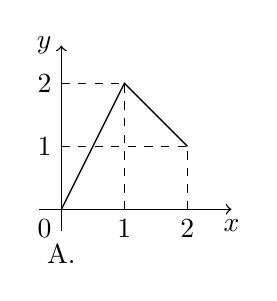
\begin{tikzpicture}[scale=0.8,line width=0.5pt]
\draw[->] (-0.35,0)--(2.7,0) node[below]{$x$};
\draw[->] (0,-0.35)--(0,2.6) node[left]{$y$};
\draw[dashed] (0,1)--(2,1) (0,2)--(1,2) (1,0)--(1,2) (2,0)--(2,1);
\draw (0,0)--(1,2)--(2,1);
\node[below left] at (0,0) {$0$};
\node[below] at (1,0) {$1$}; \node[below] at (2,0) {$2$};
\node[left] at (0,1) {$1$}; \node[left] at (0,2) {$2$};
\node[anchor=north] at (0,-0.4) {A.};
\end{tikzpicture}
&
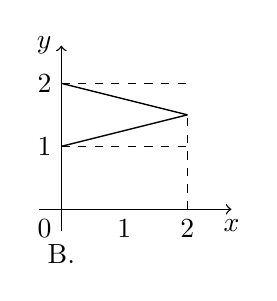
\begin{tikzpicture}[scale=0.8,line width=0.5pt]
\draw[->] (-0.35,0)--(2.7,0) node[below]{$x$};
\draw[->] (0,-0.35)--(0,2.6) node[left]{$y$};
\draw[dashed] (0,1)--(2,1) (0,2)--(2,2) (2,0)--(2,1.5);
\draw (0,2)--(2,1.5);
\draw (0,1)--(2,1.5);
\node[below left] at (0,0) {$0$};
\node[below] at (1,0) {$1$}; \node[below] at (2,0) {$2$};
\node[left] at (0,1) {$1$}; \node[left] at (0,2) {$2$};
\node[anchor=north] at (0,-0.4) {B.};
\end{tikzpicture}
\\[12pt]
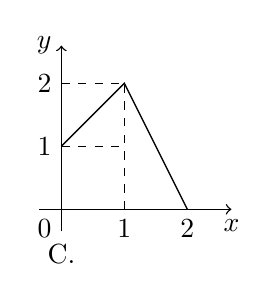
\begin{tikzpicture}[scale=0.8,line width=0.5pt]
\draw[->] (-0.35,0)--(2.7,0) node[below]{$x$};
\draw[->] (0,-0.35)--(0,2.6) node[left]{$y$};
\draw[dashed] (0,1)--(1,1) (0,2)--(1,2) (1,0)--(1,2);
\draw (0,1)--(1,2)--(2,0);
\node[below left] at (0,0) {$0$};
\node[below] at (1,0) {$1$}; \node[below] at (2,0) {$2$};
\node[left] at (0,1) {$1$}; \node[left] at (0,2) {$2$};
\node[anchor=north] at (0,-0.4) {C.};
\end{tikzpicture}
&
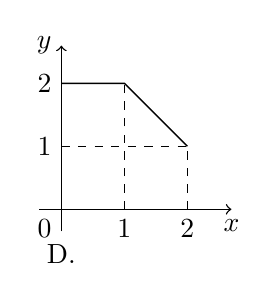
\begin{tikzpicture}[scale=0.8,line width=0.5pt]
\draw[->] (-0.35,0)--(2.7,0) node[below]{$x$};
\draw[->] (0,-0.35)--(0,2.6) node[left]{$y$};
\draw[dashed] (0,1)--(2,1) (1,0)--(1,2) (2,0)--(2,1);
\draw (0,2)--(1,2)--(2,1);
\node[below left] at (0,0) {$0$};
\node[below] at (1,0) {$1$}; \node[below] at (2,0) {$2$};
\node[left] at (0,1) {$1$}; \node[left] at (0,2) {$2$};
\node[anchor=north] at (0,-0.4) {D.};
\end{tikzpicture}
\end{tabular}
\end{center}

\ifanswer
\solbegin
\step{对于 $A$，当 $0\leqslant x\leqslant2$ 时，$0\leqslant y\leqslant2$，故 $A$ 错误；}
\step{对于 $B$，当 $0\leqslant x\leqslant2$ 时，任取一个 $x$ 的值，有两个 $y$ 与之对应，故 $B$ 错误；}
\step{对于 $C$，当 $0\leqslant x\leqslant2$ 时，$0\leqslant y\leqslant2$，故 $C$ 错误；}
\step{对于 $D$，当 $0\leqslant x\leqslant2$ 时，$0\leqslant y\leqslant2$，故 $D$ 正确.}
\step{故选 $D$.}
\solend
\fi

\item 下列函数中与函数 $y=x$ 是同一函数的是\mbox{（\quad）}

\keepwithprev
A. $y=\sqrt{x^2}$\qquad\quad B. $y=(\sqrt x)^2$\qquad\quad C. $u=\dfrac{v^2}{v}$\qquad\quad D. $m=\sqrt[5]{n^5}$

\ifanswer
\solbegin
\step{对于 $A$，$y=\sqrt{x^2}=\lvert x\rvert$，与函数 $y=x$ 的对应关系不相同，不是同一函数；}
\step{对于 $B$，$y=(\sqrt x)^2=x(x\geqslant0)$，与函数 $y=x(x\in\R)$ 的定义域不相同，不是同一函数；}
\step{对于 $C$，$u=\dfrac{v^2}{v}=v(v\neq0)$，与函数 $y=x(x\in\R)$ 的定义域不相同，不是同一函数；}
\step{对于 $D$，$m=\sqrt[5]{n^5}=n(n\in\R)$，与函数 $y=x(x\in\R)$ 的定义域相同，对应关系也相同，是同一函数.}
\step{故选 $D$.}
\solend
\fi

\item 某校高一四班学生 $46$ 人，寒假参加体育训练，其中足球队 $25$ 人，排球队 $22$ 人，游泳队 $24$ 人，足球排球都参加的有 $12$ 人，足球游泳都参加的有 $9$ 人，排球游泳都参加的有 $8$ 人，问：三项都参加的学生数为\mbox{（\quad）}

\keepwithprev
A. $2$\qquad\qquad B. $3$\qquad\qquad C. $4$\qquad\qquad D. $5$

\ifanswer
\solbegin
\step{设集合 $A=\{$参加足球队的学生$\}$，集合 $B=\{$参加排球队的学生$\}$，}
\step{集合 $C=\{$参加游泳队的学生$\}$，}
\step{则 $\operatorname{card}(A)=25$，$\operatorname{card}(B)=22$，$\operatorname{card}(C)=24$，}
\step{$\operatorname{card}(A\cap B)=12$，$\operatorname{card}(A\cap C)=9$，$\operatorname{card}(B\cap C)=8$，}
\step{设三项都参加的有 $x$ 人，即 $\operatorname{card}(A\cap B\cap C)=x$，$\operatorname{card}(A\cup B\cup C)=46$，}
\step{由 $\operatorname{card}(A\cup B\cup C)=\operatorname{card}A+\operatorname{card}B+\operatorname{card}C-\operatorname{card}(A\cap B)$}
\step{$-\operatorname{card}(B\cap C)-\operatorname{card}(A\cap C)+\operatorname{card}(A\cap B\cap C)$，}
\step{即 $46=25+22+24-12-8-9+x$，解得 $x=4$，所以三项都参加的有 $4$ 人.}
\step{故选 $C$.}
\solend
\fi

\item 已知 $\lg a$、$\lg b$ 是方程 $6x^2-4x-3=0$ 的两根，则 $\left(\lg\dfrac ab\right)^2$ 等于\mbox{（\quad）}

\keepwithprev
A. $\dfrac49$\qquad\qquad B. $\dfrac{13}{9}$\qquad\qquad C. $\dfrac{14}{9}$\qquad\qquad D. $\dfrac{22}{9}$

\ifanswer
\solbegin
\step{由韦达定理得 $\lg a+\lg b=\dfrac23$，$\lg a\cdot\lg b=-\dfrac12$，}
\step{所以 $\left(\lg\dfrac ab\right)^2=(\lg a-\lg b)^2=(\lg a+\lg b)^2-4\lg a\lg b=\dfrac49+2=\dfrac{22}{9}$. 故选 $D$.}
\solend
\fi

\end{enumerate}

\bigsec{三、解答题}

\begin{enumerate}
\setcounter{enumi}{16}

\item （1）用分数指数幂表示 $\sqrt[3]{a^2}\cdot\sqrt{a^3}$；

（2）已知 $a^{\frac12}+a^{-\frac12}=3$，求 $a+a^{-1}$.

\ifanswer
\solbegin
\step{（1）$\sqrt[3]{a^2}\cdot\sqrt{a^3}=a^{\frac23}\times a^{\frac32}=a^{\frac{13}6}$.}
\step{（2）由 $a^{\frac12}+a^{-\frac12}=3$，平方得 $a+2+a^{-1}=9$，故 $a+a^{-1}=7$.}
\solend
\fi

\item 已知 $f(x)=\begin{cases}x,x>0\\-x^2-2x+1,x\leqslant0\end{cases}$.

（1）求 $f(f(-2))$ 的值；

（2）若 $f(x_0)=2$，求 $x_0$ 的值.

\ifanswer
\solbegin
\step{（1）$f(x)=\begin{cases}x,x>0\\-x^2-2x+1,x\leqslant0\end{cases}$，则 $f(-2)=-(-2)^2-2\times(-2)+1=1$，}
\step{则有 $f(f(-2))=f(1)=1$；}
\step{（2）当 $x_0>0$ 时，$f(x_0)=x_0$，又 $f(x_0)=2$，所以 $x_0=2$，}
\step{当 $x_0\leqslant0$ 时，$f(x_0)=-x_0^2-2x_0+1$，又 $f(x_0)=2$，}
\step{所以 $-x_0^2-2x_0+1=2$，故 $x_0=-1$，}
\step{综上，$x_0$ 的值为 $-1$ 或 $2$.}
\solend
\fi

\item 已知集合 $A=\{x\mid\lvert 1+x\rvert+\lvert x\rvert<5\}$，$B=\left\{x\,\middle\vert\,\dfrac2{x-m}\geqslant1\right\}$，$p:x\in A$，$q:x\in B$.

（1）若 $m=0$，且 $p$ 真 $q$ 假，求实数 $x$ 的取值范围；

（2）若 $q$ 是 $p$ 的充分不必要条件，求实数 $m$ 的取值范围.

\ifanswer
\solbegin
\step{（1）当 $x\geqslant0$ 时，不等式 $\lvert 1+x\rvert+\lvert x\rvert<5$ 化为 $1+x+x<5$，解得 $0\leqslant x<2$；}
\step{当 $-1\leqslant x<0$ 时，不等式 $\lvert 1+x\rvert+\lvert x\rvert<5$ 化为 $1+x-x<5$ 恒成立，}
\step{故 $-1\leqslant x<0$；}
\step{当 $x<-1$ 时，不等式 $\lvert 1+x\rvert+\lvert x\rvert<5$ 化为 $-1-x-x<5$，}
\step{解得 $-3<x<-1$.}
\step{综上所述，$\lvert 1+x\rvert+\lvert x\rvert<5$ 等价于 $-3<x<2$，}
\step{所以 $\lvert 1+x\rvert+\lvert x\rvert<5$ 的解集为 $A=(-3,2)$，}
\step{若 $m=0$，则 $B=\left\{x\,\middle\vert\,\dfrac2x\geqslant1\right\}=\{x\mid 0<x\leqslant2\}$，得 $\overline{B}=(-\infty,0]\cup(2,+\infty)$，}
\step{由 $p$ 真 $q$ 假，得 $x\in(A\cap\overline{B})=(-3,0]$，即 $x$ 的取值范围为 $(-3,0]$；}
\step{（2）由 $\dfrac2{x-m}\geqslant1$，得 $\begin{cases}x-m>0\\x-m\leqslant2\end{cases}$，解得 $m<x\leqslant m+2$，}
\step{所以 $B=\left\{x\,\middle\vert\,\dfrac2{x-m}\geqslant1\right\}=(m,m+2]$，}
\step{由（1）的结论，得 $A=(-3,2)$，}
\step{若 $q$ 是 $p$ 的充分不必要条件，则 $B$ 是 $A$ 的真子集，得 $\begin{cases}m\geqslant-3\\m+2<2\end{cases}$，}
\step{解得 $-3\leqslant m<0$，即实数 $m$ 的取值范围是 $[-3,0)$.}
\solend
\fi

\item 某企业计划在 $2026$ 年布局人工智能大模型应用开发，生产智能终端配套的 $AI$ 算法服务包. 通过市场分析，全年需投入固定成本 $260$ 万元（含研发、服务器部署等），每生产 $x$ 千个算法服务包，需另投入成本 $R(x)$ 万元，且
$R(x)=\begin{cases}10x^2+100x,0<x\leqslant40\\601x+\dfrac{10000}{x}-7260,x>40\end{cases}$. 已知每个算法服务包的售价为 $0.6$ 万元，假设年内生产的服务包当年能全部销售完.

（1）试写出 $2026$ 年利润 $L$（万元）关于年产量 $x$（千个）的函数解析式；

（2）当 $2026$ 年产量为多少千个时，企业所获利润最大？并求出最大利润.

\ifanswer
\solbegin
\step{（1）$L(x)=x\cdot1000\times0.6-R(x)-260=600x-R(x)-260$，}
\step{当 $0<x\leqslant40$ 时，}
\step{$L(x)=600x-(10x^2+100x)-260=-10x^2+500x-260$；}
\step{当 $x>40$ 时，}
\step{$L(x)=600x-\left(601x+\dfrac{10000}{x}-7260\right)-260=7000-x-\dfrac{10000}{x}$；}
\step{综上，$L(x)=\begin{cases}-10x^2+500x-260,0<x\leqslant40\\7000-x-\dfrac{10000}{x},x>40\end{cases}$；}
\step{（2）当 $0<x\leqslant40$ 时，$L(x)=-10x^2+500x-260=-10(x-25)^2+5990$，}
\step{当 $x=25$ 时，函数 $L(x)$ 有最大值 $5990$；}
\step{当 $x>40$ 时，$L(x)=7000-x-\dfrac{10000}{x}=7000-\left(x+\dfrac{10000}{x}\right)$}
\step{$\leqslant7000-2\sqrt{x\cdot\dfrac{10000}{x}}=7000-2\times100=6800$，}
\step{当且仅当 $x=\dfrac{10000}{x}$ 时取等号，}
\step{所以当 $x=100$ 时，函数 $L(x)$ 有最大值 $6800$；}
\step{因为 $6800>5990$，所以 $2026$ 年产量为 $100$ 千个时，企业所获利润最大，}
\step{最大利润为 $6800$ 万元.}
\solend
\fi

\item 已知二次函数 $f(x)=ax^2+bx+c$.

（1）若 $f(x)>0$ 的解集为 $\{x\mid-3<x<4\}$，解关于 $x$ 的不等式 $bx^2+2ax-(c+3b)<0$；

（2）若函数满足 $f(x+1)-f(x)=2x+2$，且 $f(0)=1$. 求 $f(x)$ 的解析式；

（3）若对任意 $x\in\R$，不等式 $f(x)\geqslant2ax+b$ 恒成立，求 $\dfrac{b^2}{4(a^2+c^2)}$ 的最大值.

\ifanswer
\solbegin
\step{（1）由题意二次函数 $f(x)=ax^2+bx+c$，}
\step{若 $f(x)>0$ 的解集为 $\{x\mid-3<x<4\}$，}
\step{得 $-3$、$4$ 为方程 $ax^2+bx+c=0$ 的根，且 $a<0$，}
\step{则 $\begin{cases}-3+4=-\dfrac ba\\-3\times4=\dfrac ca\end{cases}$，即 $b=-a$，$c=-12a$，}
\step{则不等式 $bx^2+2ax-(c+3b)<0$，即为 $-ax^2+2ax+15a<0(a<0)$，}
\step{则 $x^2-2x-15<0$，解得 $-3<x<5$，}
\step{所以不等式 $bx^2+2ax-(c+3b)<0$ 的解集为 $(-3,5)$；}
\step{（2）由 $f(x)=ax^2+bx+c(a\neq0)$，}
\step{则 $f(x+1)-f(x)=a(x+1)^2+b(x+1)+c-(ax^2+bx+c)=2ax+a+b$，}
\step{又 $f(x+1)-f(x)=2x+2$，故 $\begin{cases}2a=2\\a+b=2\end{cases}$，解得 $a=1$，$b=1$，}
\step{由 $f(0)=1$，得 $c=1$，所以 $f(x)=x^2+x+1$；}
\step{（3）由题意二次函数 $f(x)=ax^2+bx+c$，}
\step{若对任意 $x\in\R$，不等式 $f(x)\geqslant2ax+b$ 恒成立，}
\step{得对任意 $x\in\R$，$ax^2+bx+c\geqslant2ax+b$ 恒成立，}
\step{整理得 $ax^2+(b-2a)x+c-b\geqslant0$ 恒成立，}
\step{因为 $a$ 不为 $0$，所以 $\begin{cases}a>0\\\Delta=(b-2a)^2-4a(c-b)\leqslant0\end{cases}$，}
\step{所以 $0\leqslant b^2\leqslant4a(c-a)$，所以 $\dfrac{b^2}{4(a^2+c^2)}\leqslant\dfrac{ac-a^2}{a^2+c^2}=\dfrac{\frac ca-1}{1+\left(\frac ca\right)^2}$，}
\step{令 $t=\dfrac ca-1$，因为 $0\leqslant b^2\leqslant4a(c-a)$，所以 $c\geqslant a>0\Rightarrow t\geqslant0$，}
\step{若 $t=0$ 时，此时 $\dfrac{b^2}{4(a^2+c^2)}\leqslant\dfrac{\frac ca-1}{1+\left(\frac ca\right)^2}=0$，}
\step{若 $t>0$ 时，$\dfrac{b^2}{4(a^2+c^2)}\leqslant\dfrac{t}{1+(t+1)^2}=\dfrac{t}{t^2+2t+2}=\dfrac1{t+\frac2t+2}$}
\step{$\leqslant\dfrac1{2\sqrt2+2}=\dfrac{\sqrt2-1}{2}$，}
\step{当且仅当 $t=\dfrac2t$，即 $t=\sqrt2$ 时，即 $c=(1+\sqrt2)a$ 时，上式取等号.}
\step{综上所述，$\dfrac{b^2}{4(a^2+c^2)}$ 的最大值为 $\dfrac{\sqrt2-1}{2}$.}
\solend
\fi

\end{enumerate}

\end{document}
"
% 紧凑版：xelatex "\def\iscompact{1}% 高一117_陆行中学_期中.tex
%   —— 高一上数学“2026-2027 年陆行中学高一上期中”（试卷版/答案版）
% 试卷版：xelatex 高一117_陆行中学_期中.tex
% 答案版：xelatex "\def\isanswer{1}\input{高一117_陆行中学_期中.tex}"
% 紧凑版：xelatex "\def\iscompact{1}\input{高一117_陆行中学_期中.tex}"
%
% 原始材料：微信公众号“魔都数学加油站”文章，作者破晓，2026-11-06 17:58 发布；
% 连载“27学年高一117”，原文标题“27学年高一117——2026-2027年上海市陆行中学高一上期中”；
% 原文链接：https://mp.weixin.qq.com/s/of8iPW26dvDyXWohudT0vw。
% 正文为 10 张 PNG 页（第 1、3、4、8、9、10 页 2560×3620，其余 4762×6735），
% 题目下印有【解析】或【答案】，为讲评版。
% 题目、解析均据原图转录；卷面红色水印及公众号页脚未录入。
%
% 卷首标题：原卷印作“2026-2027 年陆行中学高一上期中”（公众号标题中的“上海市”
% 卷面标题行没有，本稿照卷面），年份区间按全稿惯例排 en dash；原卷未印副标题，本稿按题目内容
% 标为“集合与常用逻辑用语、不等式、函数”（期中卷跨三章，含指数／对数与函数，与 112 同）。
%
% 与原卷的排版差异：
%   ① 原文从第 3 题起，填空题 3—12、选择题 13—16、解答题 17—21，共 19 题，本稿保留原题号；
%   ② 原卷每题下直接印【解析】／【答案】，本稿按全稿惯例置于答案版；第 4、6、8 题只印
%      【答案】，另提 \ans{}；其余选择题答案在解析末句“故选 …”，括号内留空；
%   ③ 原卷未印副标题，本稿按“知识模块”口径补出；
%   ④ 原卷填空横线按全稿惯例排为 \blankline[4.4em]；选择题括号排 \mbox{（\quad）}、
%      选项段前按惯例加 \keepwithprev；解答题不留作答区（原卷为讲评版，与 109—116 同）；
%   ⑤ 原卷 $max$／$min$ 排斜体，按 96 成例改 \max／\min；数集 $R$ 按惯例改 \R。
%
% 判别式字形：第 11 题与第 21 题 (3) 的判别式原卷排 $\Delta$（等腰、右厚），照录 \Delta。
%
% 子集符号：第 5 题的 $B\subseteq A$ 印有下划线，照录 \subseteq。
%
% 第 13 题四个坐标图选项按原图形状用 TikZ 重排（三版都出）；原卷另有第 12 题的
%   $a\odot b$ 自定义运算、第 15 题的 $\operatorname{card}$ 记号，均照录。
%
% 原卷存疑照录：第 12 题解析的 $\min\{\left|x\right|\odot\left|3-x\right|\}$ 一行、
%   第 20 题 $R(x)$ 分段函数与 $L(x)$ 的推导，均按原卷印刷行照录。
%   第 20 题题干开头原卷有一段会议背景引语（非数学信息），本稿从“某企业计划在
%   $2026$ 年布局…”起照录题目主体，全部数据、设问与解析均完整保留。
%
% 行数核对：逐题数 \step/\stepm 条数，合计 106 条（Q3：1；Q4：0；Q5：5；Q6：0；Q7：3；
% Q8：0；Q9：3；Q10：3；Q11：5；Q12：6；Q13：5；Q14：5；Q15：9；Q16：2；Q17：2；
% Q18：6；Q19：14；Q20：14；Q21：23），与原卷印刷行逐题相等（cases／TikZ 图块作一个
% 印刷行计）。第 4、6、8 题只印【答案】，提 \ans{}，不计入 \step 账。
%
\documentclass[a4paper,11pt]{article}
\usepackage{common}

\begin{document}

\examtitlest[3]{2026--2027 年陆行中学高一上期中}{集合与常用逻辑用语、不等式、函数}

\bigsec{一、填空题}

\begin{enumerate}
\setcounter{enumi}{2}

\item 已知 $10^a=2$,$10^b=5$，则 $10^{3a-2b}$ 的值为\blankline[4.4em].

\ifanswer
\solbegin
\step{$10^{3a-2b}=\dfrac{10^{3a}}{10^{2b}}=\dfrac{(10^a)^3}{(10^b)^2}=\dfrac{2^3}{5^2}=\dfrac8{25}$.}
\solend
\fi

\item 已知不等式 $\lvert x+1\rvert+\lvert x-3\rvert\geqslant4$ 恒成立，则取等号时 $x$ 的取值范围是\blankline[4.4em].

\ifanswer
\ans{$[-1,3]$}
\fi

\item 集合 $A=\{1,2,a^2\}$，$B=\{2,a\}$，若 $B\subseteq A$，则 $a$ 的值为\blankline[4.4em].

\ifanswer
\solbegin
\step{因为 $B\subseteq A$，所以 $a=1$ 或 $a=a^2$，}
\step{当 $a=1$ 时，$a^2=1$，不满足元素的互异性，故舍去；}
\step{当 $a=a^2$ 时，解得 $a=1$（舍）或 $a=0$，}
\step{当 $a=0$ 时，$A=\{1,2,0\}$，$B=\{2,0\}$，满足题意.}
\step{综上，$a=0$.}
\solend
\fi

\item 若 $x>\dfrac35$，则 $y=5x+\dfrac1{5x-3}$ 的最小值是\blankline[4.4em].

\ifanswer
\ans{$5$}
\fi

\item 已知 $a>0$，$b>0$，且 $a+b=1$，则 $\dfrac3a+\dfrac1b$ 的最小值是\blankline[4.4em].

\ifanswer
\solbegin
\step{$a>0$，$b>0$，且 $a+b=1$，}
\step{$\dfrac3a+\dfrac1b=\left(\dfrac3a+\dfrac1b\right)(a+b)=\dfrac{3b}{a}+\dfrac ab+4\geqslant2\sqrt3+4$，}
\step{当且仅当 $\dfrac{3b}{a}=\dfrac ab$ 时取等号，所以 $\dfrac3a+\dfrac1b$ 的最小值为 $2\sqrt3+4$.}
\solend
\fi

\item 已知 $\log_2 5=a$，则 $\log_5 10=$\blankline[4.4em]（用含 $a$ 的代数式表示）.

\ifanswer
\ans{$1+\dfrac1a$}
\fi

\item 已知 $p:2<x\leqslant3$，$q:\lvert x-a\rvert<2$，若 $p$ 是 $q$ 的充分不必要条件，则实数 $a$ 的取值范围为\blankline[4.4em].

\ifanswer
\solbegin
\step{由 $\lvert x-a\rvert<2$ 得 $a-2<x<a+2$，即 $p:2<x\leqslant3$，$q:a-2<x<a+2$.}
\step{因为 $p$ 是 $q$ 的充分不必要条件，所以 $\begin{cases}a-2\leqslant2\\a+2>3\end{cases}$，解得 $1<a\leqslant4$，}
\step{所以实数 $a$ 的取值范围为 $(1,4]$.}
\solend
\fi

\item 已知 $a>1$,$b>1$，若 $\log_a b+\log_b a=2$，且 $ab=2$，则 $\log_2(a+b)=$\blankline[4.4em].

\ifanswer
\solbegin
\step{由 $\log_a b+\log_b a=2$,$a>1$,$b>1$，得 $\log_a b+\dfrac1{\log_a b}=2$，}
\step{即 $(\log_a b)^2-2\log_a b+1=0$，则 $(\log_a b-1)^2=0$，即 $\log_a b=1$，则 $a=b$，}
\step{又 $ab=2$，则 $a=b=\sqrt2$，所以 $\log_2(a+b)=\log_2(2\sqrt2)=\log_2 2^{\frac32}=\dfrac32$.}
\solend
\fi

\item 已知函数 $f(x)=\sqrt{2kx^2+kx+\dfrac34}$ 的定义域为实数集 $\R$，则实数 $k$ 的取值范围\blankline[4.4em].

\ifanswer
\solbegin
\step{因为函数 $f(x)=\sqrt{2kx^2+kx+\dfrac34}$ 的定义域为实数集 $\R$，}
\step{所以 $2kx^2+kx+\dfrac34\geqslant0$ 在 $\R$ 上恒成立，}
\step{当 $k=0$ 时，$\dfrac34\geqslant0$，恒成立；}
\step{当 $k\neq0$ 时，则有 $\begin{cases}2k>0\\\Delta=k^2-4\times2k\times\dfrac34\leqslant0\end{cases}$，解得 $0<k\leqslant6$；}
\step{综上，实数 $k$ 的取值范围为 $[0,6]$.}
\solend
\fi

\item 对于两个实数 $a$、$b$，定义运算 $a\odot b$ 如下：若 $a\geqslant b$，则 $a\odot b=a$；若 $a<b$，则 $a\odot b=b$. 若 $x$、$y\in\R$，则 $\lvert x-y\rvert\odot\lvert 3-x\rvert\odot\lvert x+y\rvert$ 的最小值是\blankline[4.4em].

\ifanswer
\solbegin
\step{由题意得 $a\odot b=\max\{a,b\}$，所以 $\lvert a+b\rvert\odot\lvert a-b\rvert=\max\{\lvert a+b\rvert,\lvert a-b\rvert\}$，}
\step{设 $\max\{\lvert a+b\rvert,\lvert a-b\rvert\}=M$，则 $\begin{cases}M\geqslant\lvert a+b\rvert\\M\geqslant\lvert a-b\rvert\end{cases}$，}
\step{所以 $2M\geqslant\lvert a+b\rvert+\lvert a-b\rvert\geqslant2\lvert a\rvert$，则 $\lvert a+b\rvert\odot\lvert a-b\rvert\geqslant\lvert a\rvert$，}
\step{所以 $\min\{\lvert x-y\rvert\odot\lvert 3-x\rvert\odot\lvert x+y\rvert\}=\min\{\lvert x-y\rvert\odot\lvert x+y\rvert\odot\lvert 3-x\rvert\}$}
\step{$=\min\{\lvert x\rvert\odot\lvert 3-x\rvert\}=\min\left\{\dfrac32+x\odot\left\lvert\dfrac32-x\right\rvert\right\}=\dfrac32$，}% 原卷该行写法照录
\step{当且仅当 $x=\dfrac32$，$y=0$ 取等号，故 $\lvert x-y\rvert\odot\lvert 3-x\rvert\odot\lvert x+y\rvert$ 的最小值是 $\dfrac32$.}
\solend
\fi

\end{enumerate}

\bigsec{二、选择题}

\begin{enumerate}
\setcounter{enumi}{12}

\item 设 $A=\{x\mid 0\leqslant x\leqslant2\}$，$B=\{y\mid 1\leqslant y\leqslant2\}$，下列图形能表示从集合 $A$ 到集合 $B$ 的函数图像的是\mbox{（\quad）}

\keepwithprev
\begin{center}
% 原卷四个坐标图选项按原图形状用 TikZ 重排。
\begin{tabular}{c@{\qquad\qquad}c}
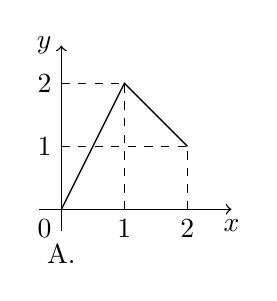
\begin{tikzpicture}[scale=0.8,line width=0.5pt]
\draw[->] (-0.35,0)--(2.7,0) node[below]{$x$};
\draw[->] (0,-0.35)--(0,2.6) node[left]{$y$};
\draw[dashed] (0,1)--(2,1) (0,2)--(1,2) (1,0)--(1,2) (2,0)--(2,1);
\draw (0,0)--(1,2)--(2,1);
\node[below left] at (0,0) {$0$};
\node[below] at (1,0) {$1$}; \node[below] at (2,0) {$2$};
\node[left] at (0,1) {$1$}; \node[left] at (0,2) {$2$};
\node[anchor=north] at (0,-0.4) {A.};
\end{tikzpicture}
&
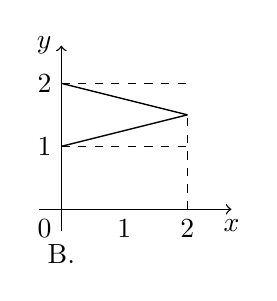
\begin{tikzpicture}[scale=0.8,line width=0.5pt]
\draw[->] (-0.35,0)--(2.7,0) node[below]{$x$};
\draw[->] (0,-0.35)--(0,2.6) node[left]{$y$};
\draw[dashed] (0,1)--(2,1) (0,2)--(2,2) (2,0)--(2,1.5);
\draw (0,2)--(2,1.5);
\draw (0,1)--(2,1.5);
\node[below left] at (0,0) {$0$};
\node[below] at (1,0) {$1$}; \node[below] at (2,0) {$2$};
\node[left] at (0,1) {$1$}; \node[left] at (0,2) {$2$};
\node[anchor=north] at (0,-0.4) {B.};
\end{tikzpicture}
\\[12pt]
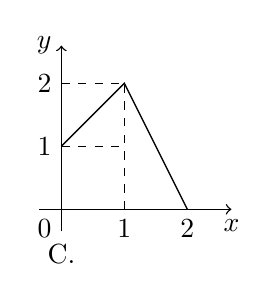
\begin{tikzpicture}[scale=0.8,line width=0.5pt]
\draw[->] (-0.35,0)--(2.7,0) node[below]{$x$};
\draw[->] (0,-0.35)--(0,2.6) node[left]{$y$};
\draw[dashed] (0,1)--(1,1) (0,2)--(1,2) (1,0)--(1,2);
\draw (0,1)--(1,2)--(2,0);
\node[below left] at (0,0) {$0$};
\node[below] at (1,0) {$1$}; \node[below] at (2,0) {$2$};
\node[left] at (0,1) {$1$}; \node[left] at (0,2) {$2$};
\node[anchor=north] at (0,-0.4) {C.};
\end{tikzpicture}
&
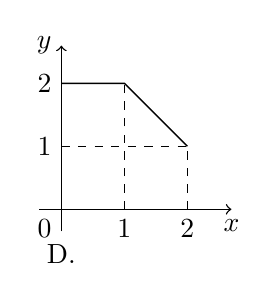
\begin{tikzpicture}[scale=0.8,line width=0.5pt]
\draw[->] (-0.35,0)--(2.7,0) node[below]{$x$};
\draw[->] (0,-0.35)--(0,2.6) node[left]{$y$};
\draw[dashed] (0,1)--(2,1) (1,0)--(1,2) (2,0)--(2,1);
\draw (0,2)--(1,2)--(2,1);
\node[below left] at (0,0) {$0$};
\node[below] at (1,0) {$1$}; \node[below] at (2,0) {$2$};
\node[left] at (0,1) {$1$}; \node[left] at (0,2) {$2$};
\node[anchor=north] at (0,-0.4) {D.};
\end{tikzpicture}
\end{tabular}
\end{center}

\ifanswer
\solbegin
\step{对于 $A$，当 $0\leqslant x\leqslant2$ 时，$0\leqslant y\leqslant2$，故 $A$ 错误；}
\step{对于 $B$，当 $0\leqslant x\leqslant2$ 时，任取一个 $x$ 的值，有两个 $y$ 与之对应，故 $B$ 错误；}
\step{对于 $C$，当 $0\leqslant x\leqslant2$ 时，$0\leqslant y\leqslant2$，故 $C$ 错误；}
\step{对于 $D$，当 $0\leqslant x\leqslant2$ 时，$0\leqslant y\leqslant2$，故 $D$ 正确.}
\step{故选 $D$.}
\solend
\fi

\item 下列函数中与函数 $y=x$ 是同一函数的是\mbox{（\quad）}

\keepwithprev
A. $y=\sqrt{x^2}$\qquad\quad B. $y=(\sqrt x)^2$\qquad\quad C. $u=\dfrac{v^2}{v}$\qquad\quad D. $m=\sqrt[5]{n^5}$

\ifanswer
\solbegin
\step{对于 $A$，$y=\sqrt{x^2}=\lvert x\rvert$，与函数 $y=x$ 的对应关系不相同，不是同一函数；}
\step{对于 $B$，$y=(\sqrt x)^2=x(x\geqslant0)$，与函数 $y=x(x\in\R)$ 的定义域不相同，不是同一函数；}
\step{对于 $C$，$u=\dfrac{v^2}{v}=v(v\neq0)$，与函数 $y=x(x\in\R)$ 的定义域不相同，不是同一函数；}
\step{对于 $D$，$m=\sqrt[5]{n^5}=n(n\in\R)$，与函数 $y=x(x\in\R)$ 的定义域相同，对应关系也相同，是同一函数.}
\step{故选 $D$.}
\solend
\fi

\item 某校高一四班学生 $46$ 人，寒假参加体育训练，其中足球队 $25$ 人，排球队 $22$ 人，游泳队 $24$ 人，足球排球都参加的有 $12$ 人，足球游泳都参加的有 $9$ 人，排球游泳都参加的有 $8$ 人，问：三项都参加的学生数为\mbox{（\quad）}

\keepwithprev
A. $2$\qquad\qquad B. $3$\qquad\qquad C. $4$\qquad\qquad D. $5$

\ifanswer
\solbegin
\step{设集合 $A=\{$参加足球队的学生$\}$，集合 $B=\{$参加排球队的学生$\}$，}
\step{集合 $C=\{$参加游泳队的学生$\}$，}
\step{则 $\operatorname{card}(A)=25$，$\operatorname{card}(B)=22$，$\operatorname{card}(C)=24$，}
\step{$\operatorname{card}(A\cap B)=12$，$\operatorname{card}(A\cap C)=9$，$\operatorname{card}(B\cap C)=8$，}
\step{设三项都参加的有 $x$ 人，即 $\operatorname{card}(A\cap B\cap C)=x$，$\operatorname{card}(A\cup B\cup C)=46$，}
\step{由 $\operatorname{card}(A\cup B\cup C)=\operatorname{card}A+\operatorname{card}B+\operatorname{card}C-\operatorname{card}(A\cap B)$}
\step{$-\operatorname{card}(B\cap C)-\operatorname{card}(A\cap C)+\operatorname{card}(A\cap B\cap C)$，}
\step{即 $46=25+22+24-12-8-9+x$，解得 $x=4$，所以三项都参加的有 $4$ 人.}
\step{故选 $C$.}
\solend
\fi

\item 已知 $\lg a$、$\lg b$ 是方程 $6x^2-4x-3=0$ 的两根，则 $\left(\lg\dfrac ab\right)^2$ 等于\mbox{（\quad）}

\keepwithprev
A. $\dfrac49$\qquad\qquad B. $\dfrac{13}{9}$\qquad\qquad C. $\dfrac{14}{9}$\qquad\qquad D. $\dfrac{22}{9}$

\ifanswer
\solbegin
\step{由韦达定理得 $\lg a+\lg b=\dfrac23$，$\lg a\cdot\lg b=-\dfrac12$，}
\step{所以 $\left(\lg\dfrac ab\right)^2=(\lg a-\lg b)^2=(\lg a+\lg b)^2-4\lg a\lg b=\dfrac49+2=\dfrac{22}{9}$. 故选 $D$.}
\solend
\fi

\end{enumerate}

\bigsec{三、解答题}

\begin{enumerate}
\setcounter{enumi}{16}

\item （1）用分数指数幂表示 $\sqrt[3]{a^2}\cdot\sqrt{a^3}$；

（2）已知 $a^{\frac12}+a^{-\frac12}=3$，求 $a+a^{-1}$.

\ifanswer
\solbegin
\step{（1）$\sqrt[3]{a^2}\cdot\sqrt{a^3}=a^{\frac23}\times a^{\frac32}=a^{\frac{13}6}$.}
\step{（2）由 $a^{\frac12}+a^{-\frac12}=3$，平方得 $a+2+a^{-1}=9$，故 $a+a^{-1}=7$.}
\solend
\fi

\item 已知 $f(x)=\begin{cases}x,x>0\\-x^2-2x+1,x\leqslant0\end{cases}$.

（1）求 $f(f(-2))$ 的值；

（2）若 $f(x_0)=2$，求 $x_0$ 的值.

\ifanswer
\solbegin
\step{（1）$f(x)=\begin{cases}x,x>0\\-x^2-2x+1,x\leqslant0\end{cases}$，则 $f(-2)=-(-2)^2-2\times(-2)+1=1$，}
\step{则有 $f(f(-2))=f(1)=1$；}
\step{（2）当 $x_0>0$ 时，$f(x_0)=x_0$，又 $f(x_0)=2$，所以 $x_0=2$，}
\step{当 $x_0\leqslant0$ 时，$f(x_0)=-x_0^2-2x_0+1$，又 $f(x_0)=2$，}
\step{所以 $-x_0^2-2x_0+1=2$，故 $x_0=-1$，}
\step{综上，$x_0$ 的值为 $-1$ 或 $2$.}
\solend
\fi

\item 已知集合 $A=\{x\mid\lvert 1+x\rvert+\lvert x\rvert<5\}$，$B=\left\{x\,\middle\vert\,\dfrac2{x-m}\geqslant1\right\}$，$p:x\in A$，$q:x\in B$.

（1）若 $m=0$，且 $p$ 真 $q$ 假，求实数 $x$ 的取值范围；

（2）若 $q$ 是 $p$ 的充分不必要条件，求实数 $m$ 的取值范围.

\ifanswer
\solbegin
\step{（1）当 $x\geqslant0$ 时，不等式 $\lvert 1+x\rvert+\lvert x\rvert<5$ 化为 $1+x+x<5$，解得 $0\leqslant x<2$；}
\step{当 $-1\leqslant x<0$ 时，不等式 $\lvert 1+x\rvert+\lvert x\rvert<5$ 化为 $1+x-x<5$ 恒成立，}
\step{故 $-1\leqslant x<0$；}
\step{当 $x<-1$ 时，不等式 $\lvert 1+x\rvert+\lvert x\rvert<5$ 化为 $-1-x-x<5$，}
\step{解得 $-3<x<-1$.}
\step{综上所述，$\lvert 1+x\rvert+\lvert x\rvert<5$ 等价于 $-3<x<2$，}
\step{所以 $\lvert 1+x\rvert+\lvert x\rvert<5$ 的解集为 $A=(-3,2)$，}
\step{若 $m=0$，则 $B=\left\{x\,\middle\vert\,\dfrac2x\geqslant1\right\}=\{x\mid 0<x\leqslant2\}$，得 $\overline{B}=(-\infty,0]\cup(2,+\infty)$，}
\step{由 $p$ 真 $q$ 假，得 $x\in(A\cap\overline{B})=(-3,0]$，即 $x$ 的取值范围为 $(-3,0]$；}
\step{（2）由 $\dfrac2{x-m}\geqslant1$，得 $\begin{cases}x-m>0\\x-m\leqslant2\end{cases}$，解得 $m<x\leqslant m+2$，}
\step{所以 $B=\left\{x\,\middle\vert\,\dfrac2{x-m}\geqslant1\right\}=(m,m+2]$，}
\step{由（1）的结论，得 $A=(-3,2)$，}
\step{若 $q$ 是 $p$ 的充分不必要条件，则 $B$ 是 $A$ 的真子集，得 $\begin{cases}m\geqslant-3\\m+2<2\end{cases}$，}
\step{解得 $-3\leqslant m<0$，即实数 $m$ 的取值范围是 $[-3,0)$.}
\solend
\fi

\item 某企业计划在 $2026$ 年布局人工智能大模型应用开发，生产智能终端配套的 $AI$ 算法服务包. 通过市场分析，全年需投入固定成本 $260$ 万元（含研发、服务器部署等），每生产 $x$ 千个算法服务包，需另投入成本 $R(x)$ 万元，且
$R(x)=\begin{cases}10x^2+100x,0<x\leqslant40\\601x+\dfrac{10000}{x}-7260,x>40\end{cases}$. 已知每个算法服务包的售价为 $0.6$ 万元，假设年内生产的服务包当年能全部销售完.

（1）试写出 $2026$ 年利润 $L$（万元）关于年产量 $x$（千个）的函数解析式；

（2）当 $2026$ 年产量为多少千个时，企业所获利润最大？并求出最大利润.

\ifanswer
\solbegin
\step{（1）$L(x)=x\cdot1000\times0.6-R(x)-260=600x-R(x)-260$，}
\step{当 $0<x\leqslant40$ 时，}
\step{$L(x)=600x-(10x^2+100x)-260=-10x^2+500x-260$；}
\step{当 $x>40$ 时，}
\step{$L(x)=600x-\left(601x+\dfrac{10000}{x}-7260\right)-260=7000-x-\dfrac{10000}{x}$；}
\step{综上，$L(x)=\begin{cases}-10x^2+500x-260,0<x\leqslant40\\7000-x-\dfrac{10000}{x},x>40\end{cases}$；}
\step{（2）当 $0<x\leqslant40$ 时，$L(x)=-10x^2+500x-260=-10(x-25)^2+5990$，}
\step{当 $x=25$ 时，函数 $L(x)$ 有最大值 $5990$；}
\step{当 $x>40$ 时，$L(x)=7000-x-\dfrac{10000}{x}=7000-\left(x+\dfrac{10000}{x}\right)$}
\step{$\leqslant7000-2\sqrt{x\cdot\dfrac{10000}{x}}=7000-2\times100=6800$，}
\step{当且仅当 $x=\dfrac{10000}{x}$ 时取等号，}
\step{所以当 $x=100$ 时，函数 $L(x)$ 有最大值 $6800$；}
\step{因为 $6800>5990$，所以 $2026$ 年产量为 $100$ 千个时，企业所获利润最大，}
\step{最大利润为 $6800$ 万元.}
\solend
\fi

\item 已知二次函数 $f(x)=ax^2+bx+c$.

（1）若 $f(x)>0$ 的解集为 $\{x\mid-3<x<4\}$，解关于 $x$ 的不等式 $bx^2+2ax-(c+3b)<0$；

（2）若函数满足 $f(x+1)-f(x)=2x+2$，且 $f(0)=1$. 求 $f(x)$ 的解析式；

（3）若对任意 $x\in\R$，不等式 $f(x)\geqslant2ax+b$ 恒成立，求 $\dfrac{b^2}{4(a^2+c^2)}$ 的最大值.

\ifanswer
\solbegin
\step{（1）由题意二次函数 $f(x)=ax^2+bx+c$，}
\step{若 $f(x)>0$ 的解集为 $\{x\mid-3<x<4\}$，}
\step{得 $-3$、$4$ 为方程 $ax^2+bx+c=0$ 的根，且 $a<0$，}
\step{则 $\begin{cases}-3+4=-\dfrac ba\\-3\times4=\dfrac ca\end{cases}$，即 $b=-a$，$c=-12a$，}
\step{则不等式 $bx^2+2ax-(c+3b)<0$，即为 $-ax^2+2ax+15a<0(a<0)$，}
\step{则 $x^2-2x-15<0$，解得 $-3<x<5$，}
\step{所以不等式 $bx^2+2ax-(c+3b)<0$ 的解集为 $(-3,5)$；}
\step{（2）由 $f(x)=ax^2+bx+c(a\neq0)$，}
\step{则 $f(x+1)-f(x)=a(x+1)^2+b(x+1)+c-(ax^2+bx+c)=2ax+a+b$，}
\step{又 $f(x+1)-f(x)=2x+2$，故 $\begin{cases}2a=2\\a+b=2\end{cases}$，解得 $a=1$，$b=1$，}
\step{由 $f(0)=1$，得 $c=1$，所以 $f(x)=x^2+x+1$；}
\step{（3）由题意二次函数 $f(x)=ax^2+bx+c$，}
\step{若对任意 $x\in\R$，不等式 $f(x)\geqslant2ax+b$ 恒成立，}
\step{得对任意 $x\in\R$，$ax^2+bx+c\geqslant2ax+b$ 恒成立，}
\step{整理得 $ax^2+(b-2a)x+c-b\geqslant0$ 恒成立，}
\step{因为 $a$ 不为 $0$，所以 $\begin{cases}a>0\\\Delta=(b-2a)^2-4a(c-b)\leqslant0\end{cases}$，}
\step{所以 $0\leqslant b^2\leqslant4a(c-a)$，所以 $\dfrac{b^2}{4(a^2+c^2)}\leqslant\dfrac{ac-a^2}{a^2+c^2}=\dfrac{\frac ca-1}{1+\left(\frac ca\right)^2}$，}
\step{令 $t=\dfrac ca-1$，因为 $0\leqslant b^2\leqslant4a(c-a)$，所以 $c\geqslant a>0\Rightarrow t\geqslant0$，}
\step{若 $t=0$ 时，此时 $\dfrac{b^2}{4(a^2+c^2)}\leqslant\dfrac{\frac ca-1}{1+\left(\frac ca\right)^2}=0$，}
\step{若 $t>0$ 时，$\dfrac{b^2}{4(a^2+c^2)}\leqslant\dfrac{t}{1+(t+1)^2}=\dfrac{t}{t^2+2t+2}=\dfrac1{t+\frac2t+2}$}
\step{$\leqslant\dfrac1{2\sqrt2+2}=\dfrac{\sqrt2-1}{2}$，}
\step{当且仅当 $t=\dfrac2t$，即 $t=\sqrt2$ 时，即 $c=(1+\sqrt2)a$ 时，上式取等号.}
\step{综上所述，$\dfrac{b^2}{4(a^2+c^2)}$ 的最大值为 $\dfrac{\sqrt2-1}{2}$.}
\solend
\fi

\end{enumerate}

\end{document}
"
%
% 原始材料：微信公众号“魔都数学加油站”文章，作者破晓，2026-11-06 17:58 发布；
% 连载“27学年高一117”，原文标题“27学年高一117——2026-2027年上海市陆行中学高一上期中”；
% 原文链接：https://mp.weixin.qq.com/s/of8iPW26dvDyXWohudT0vw。
% 正文为 10 张 PNG 页（第 1、3、4、8、9、10 页 2560×3620，其余 4762×6735），
% 题目下印有【解析】或【答案】，为讲评版。
% 题目、解析均据原图转录；卷面红色水印及公众号页脚未录入。
%
% 卷首标题：原卷印作“2026-2027 年陆行中学高一上期中”（公众号标题中的“上海市”
% 卷面标题行没有，本稿照卷面），年份区间按全稿惯例排 en dash；原卷未印副标题，本稿按题目内容
% 标为“集合与常用逻辑用语、不等式、函数”（期中卷跨三章，含指数／对数与函数，与 112 同）。
%
% 与原卷的排版差异：
%   ① 原文从第 3 题起，填空题 3—12、选择题 13—16、解答题 17—21，共 19 题，本稿保留原题号；
%   ② 原卷每题下直接印【解析】／【答案】，本稿按全稿惯例置于答案版；第 4、6、8 题只印
%      【答案】，另提 \ans{}；其余选择题答案在解析末句“故选 …”，括号内留空；
%   ③ 原卷未印副标题，本稿按“知识模块”口径补出；
%   ④ 原卷填空横线按全稿惯例排为 \blankline[4.4em]；选择题括号排 \mbox{（\quad）}、
%      选项段前按惯例加 \keepwithprev；解答题不留作答区（原卷为讲评版，与 109—116 同）；
%   ⑤ 原卷 $max$／$min$ 排斜体，按 96 成例改 \max／\min；数集 $R$ 按惯例改 \R。
%
% 判别式字形：第 11 题与第 21 题 (3) 的判别式原卷排 $\Delta$（等腰、右厚），照录 \Delta。
%
% 子集符号：第 5 题的 $B\subseteq A$ 印有下划线，照录 \subseteq。
%
% 第 13 题四个坐标图选项按原图形状用 TikZ 重排（三版都出）；原卷另有第 12 题的
%   $a\odot b$ 自定义运算、第 15 题的 $\operatorname{card}$ 记号，均照录。
%
% 原卷存疑照录：第 12 题解析的 $\min\{\left|x\right|\odot\left|3-x\right|\}$ 一行、
%   第 20 题 $R(x)$ 分段函数与 $L(x)$ 的推导，均按原卷印刷行照录。
%   第 20 题题干开头原卷有一段会议背景引语（非数学信息），本稿从“某企业计划在
%   $2026$ 年布局…”起照录题目主体，全部数据、设问与解析均完整保留。
%
% 行数核对：逐题数 \step/\stepm 条数，合计 106 条（Q3：1；Q4：0；Q5：5；Q6：0；Q7：3；
% Q8：0；Q9：3；Q10：3；Q11：5；Q12：6；Q13：5；Q14：5；Q15：9；Q16：2；Q17：2；
% Q18：6；Q19：14；Q20：14；Q21：23），与原卷印刷行逐题相等（cases／TikZ 图块作一个
% 印刷行计）。第 4、6、8 题只印【答案】，提 \ans{}，不计入 \step 账。
%
\documentclass[a4paper,11pt]{article}
\usepackage{common}

\begin{document}

\examtitlest[3]{2026--2027 年陆行中学高一上期中}{集合与常用逻辑用语、不等式、函数}

\bigsec{一、填空题}

\begin{enumerate}
\setcounter{enumi}{2}

\item 已知 $10^a=2$,$10^b=5$，则 $10^{3a-2b}$ 的值为\blankline[4.4em].

\ifanswer
\solbegin
\step{$10^{3a-2b}=\dfrac{10^{3a}}{10^{2b}}=\dfrac{(10^a)^3}{(10^b)^2}=\dfrac{2^3}{5^2}=\dfrac8{25}$.}
\solend
\fi

\item 已知不等式 $\lvert x+1\rvert+\lvert x-3\rvert\geqslant4$ 恒成立，则取等号时 $x$ 的取值范围是\blankline[4.4em].

\ifanswer
\ans{$[-1,3]$}
\fi

\item 集合 $A=\{1,2,a^2\}$，$B=\{2,a\}$，若 $B\subseteq A$，则 $a$ 的值为\blankline[4.4em].

\ifanswer
\solbegin
\step{因为 $B\subseteq A$，所以 $a=1$ 或 $a=a^2$，}
\step{当 $a=1$ 时，$a^2=1$，不满足元素的互异性，故舍去；}
\step{当 $a=a^2$ 时，解得 $a=1$（舍）或 $a=0$，}
\step{当 $a=0$ 时，$A=\{1,2,0\}$，$B=\{2,0\}$，满足题意.}
\step{综上，$a=0$.}
\solend
\fi

\item 若 $x>\dfrac35$，则 $y=5x+\dfrac1{5x-3}$ 的最小值是\blankline[4.4em].

\ifanswer
\ans{$5$}
\fi

\item 已知 $a>0$，$b>0$，且 $a+b=1$，则 $\dfrac3a+\dfrac1b$ 的最小值是\blankline[4.4em].

\ifanswer
\solbegin
\step{$a>0$，$b>0$，且 $a+b=1$，}
\step{$\dfrac3a+\dfrac1b=\left(\dfrac3a+\dfrac1b\right)(a+b)=\dfrac{3b}{a}+\dfrac ab+4\geqslant2\sqrt3+4$，}
\step{当且仅当 $\dfrac{3b}{a}=\dfrac ab$ 时取等号，所以 $\dfrac3a+\dfrac1b$ 的最小值为 $2\sqrt3+4$.}
\solend
\fi

\item 已知 $\log_2 5=a$，则 $\log_5 10=$\blankline[4.4em]（用含 $a$ 的代数式表示）.

\ifanswer
\ans{$1+\dfrac1a$}
\fi

\item 已知 $p:2<x\leqslant3$，$q:\lvert x-a\rvert<2$，若 $p$ 是 $q$ 的充分不必要条件，则实数 $a$ 的取值范围为\blankline[4.4em].

\ifanswer
\solbegin
\step{由 $\lvert x-a\rvert<2$ 得 $a-2<x<a+2$，即 $p:2<x\leqslant3$，$q:a-2<x<a+2$.}
\step{因为 $p$ 是 $q$ 的充分不必要条件，所以 $\begin{cases}a-2\leqslant2\\a+2>3\end{cases}$，解得 $1<a\leqslant4$，}
\step{所以实数 $a$ 的取值范围为 $(1,4]$.}
\solend
\fi

\item 已知 $a>1$,$b>1$，若 $\log_a b+\log_b a=2$，且 $ab=2$，则 $\log_2(a+b)=$\blankline[4.4em].

\ifanswer
\solbegin
\step{由 $\log_a b+\log_b a=2$,$a>1$,$b>1$，得 $\log_a b+\dfrac1{\log_a b}=2$，}
\step{即 $(\log_a b)^2-2\log_a b+1=0$，则 $(\log_a b-1)^2=0$，即 $\log_a b=1$，则 $a=b$，}
\step{又 $ab=2$，则 $a=b=\sqrt2$，所以 $\log_2(a+b)=\log_2(2\sqrt2)=\log_2 2^{\frac32}=\dfrac32$.}
\solend
\fi

\item 已知函数 $f(x)=\sqrt{2kx^2+kx+\dfrac34}$ 的定义域为实数集 $\R$，则实数 $k$ 的取值范围\blankline[4.4em].

\ifanswer
\solbegin
\step{因为函数 $f(x)=\sqrt{2kx^2+kx+\dfrac34}$ 的定义域为实数集 $\R$，}
\step{所以 $2kx^2+kx+\dfrac34\geqslant0$ 在 $\R$ 上恒成立，}
\step{当 $k=0$ 时，$\dfrac34\geqslant0$，恒成立；}
\step{当 $k\neq0$ 时，则有 $\begin{cases}2k>0\\\Delta=k^2-4\times2k\times\dfrac34\leqslant0\end{cases}$，解得 $0<k\leqslant6$；}
\step{综上，实数 $k$ 的取值范围为 $[0,6]$.}
\solend
\fi

\item 对于两个实数 $a$、$b$，定义运算 $a\odot b$ 如下：若 $a\geqslant b$，则 $a\odot b=a$；若 $a<b$，则 $a\odot b=b$. 若 $x$、$y\in\R$，则 $\lvert x-y\rvert\odot\lvert 3-x\rvert\odot\lvert x+y\rvert$ 的最小值是\blankline[4.4em].

\ifanswer
\solbegin
\step{由题意得 $a\odot b=\max\{a,b\}$，所以 $\lvert a+b\rvert\odot\lvert a-b\rvert=\max\{\lvert a+b\rvert,\lvert a-b\rvert\}$，}
\step{设 $\max\{\lvert a+b\rvert,\lvert a-b\rvert\}=M$，则 $\begin{cases}M\geqslant\lvert a+b\rvert\\M\geqslant\lvert a-b\rvert\end{cases}$，}
\step{所以 $2M\geqslant\lvert a+b\rvert+\lvert a-b\rvert\geqslant2\lvert a\rvert$，则 $\lvert a+b\rvert\odot\lvert a-b\rvert\geqslant\lvert a\rvert$，}
\step{所以 $\min\{\lvert x-y\rvert\odot\lvert 3-x\rvert\odot\lvert x+y\rvert\}=\min\{\lvert x-y\rvert\odot\lvert x+y\rvert\odot\lvert 3-x\rvert\}$}
\step{$=\min\{\lvert x\rvert\odot\lvert 3-x\rvert\}=\min\left\{\dfrac32+x\odot\left\lvert\dfrac32-x\right\rvert\right\}=\dfrac32$，}% 原卷该行写法照录
\step{当且仅当 $x=\dfrac32$，$y=0$ 取等号，故 $\lvert x-y\rvert\odot\lvert 3-x\rvert\odot\lvert x+y\rvert$ 的最小值是 $\dfrac32$.}
\solend
\fi

\end{enumerate}

\bigsec{二、选择题}

\begin{enumerate}
\setcounter{enumi}{12}

\item 设 $A=\{x\mid 0\leqslant x\leqslant2\}$，$B=\{y\mid 1\leqslant y\leqslant2\}$，下列图形能表示从集合 $A$ 到集合 $B$ 的函数图像的是\mbox{（\quad）}

\keepwithprev
\begin{center}
% 原卷四个坐标图选项按原图形状用 TikZ 重排。
\begin{tabular}{c@{\qquad\qquad}c}
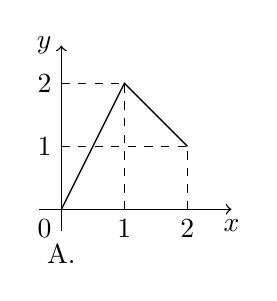
\begin{tikzpicture}[scale=0.8,line width=0.5pt]
\draw[->] (-0.35,0)--(2.7,0) node[below]{$x$};
\draw[->] (0,-0.35)--(0,2.6) node[left]{$y$};
\draw[dashed] (0,1)--(2,1) (0,2)--(1,2) (1,0)--(1,2) (2,0)--(2,1);
\draw (0,0)--(1,2)--(2,1);
\node[below left] at (0,0) {$0$};
\node[below] at (1,0) {$1$}; \node[below] at (2,0) {$2$};
\node[left] at (0,1) {$1$}; \node[left] at (0,2) {$2$};
\node[anchor=north] at (0,-0.4) {A.};
\end{tikzpicture}
&
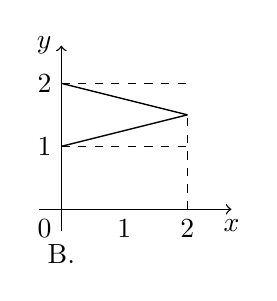
\begin{tikzpicture}[scale=0.8,line width=0.5pt]
\draw[->] (-0.35,0)--(2.7,0) node[below]{$x$};
\draw[->] (0,-0.35)--(0,2.6) node[left]{$y$};
\draw[dashed] (0,1)--(2,1) (0,2)--(2,2) (2,0)--(2,1.5);
\draw (0,2)--(2,1.5);
\draw (0,1)--(2,1.5);
\node[below left] at (0,0) {$0$};
\node[below] at (1,0) {$1$}; \node[below] at (2,0) {$2$};
\node[left] at (0,1) {$1$}; \node[left] at (0,2) {$2$};
\node[anchor=north] at (0,-0.4) {B.};
\end{tikzpicture}
\\[12pt]
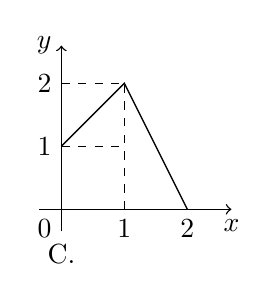
\begin{tikzpicture}[scale=0.8,line width=0.5pt]
\draw[->] (-0.35,0)--(2.7,0) node[below]{$x$};
\draw[->] (0,-0.35)--(0,2.6) node[left]{$y$};
\draw[dashed] (0,1)--(1,1) (0,2)--(1,2) (1,0)--(1,2);
\draw (0,1)--(1,2)--(2,0);
\node[below left] at (0,0) {$0$};
\node[below] at (1,0) {$1$}; \node[below] at (2,0) {$2$};
\node[left] at (0,1) {$1$}; \node[left] at (0,2) {$2$};
\node[anchor=north] at (0,-0.4) {C.};
\end{tikzpicture}
&
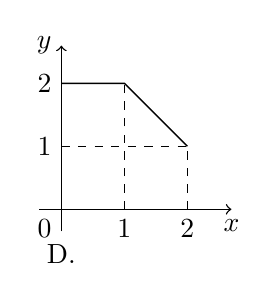
\begin{tikzpicture}[scale=0.8,line width=0.5pt]
\draw[->] (-0.35,0)--(2.7,0) node[below]{$x$};
\draw[->] (0,-0.35)--(0,2.6) node[left]{$y$};
\draw[dashed] (0,1)--(2,1) (1,0)--(1,2) (2,0)--(2,1);
\draw (0,2)--(1,2)--(2,1);
\node[below left] at (0,0) {$0$};
\node[below] at (1,0) {$1$}; \node[below] at (2,0) {$2$};
\node[left] at (0,1) {$1$}; \node[left] at (0,2) {$2$};
\node[anchor=north] at (0,-0.4) {D.};
\end{tikzpicture}
\end{tabular}
\end{center}

\ifanswer
\solbegin
\step{对于 $A$，当 $0\leqslant x\leqslant2$ 时，$0\leqslant y\leqslant2$，故 $A$ 错误；}
\step{对于 $B$，当 $0\leqslant x\leqslant2$ 时，任取一个 $x$ 的值，有两个 $y$ 与之对应，故 $B$ 错误；}
\step{对于 $C$，当 $0\leqslant x\leqslant2$ 时，$0\leqslant y\leqslant2$，故 $C$ 错误；}
\step{对于 $D$，当 $0\leqslant x\leqslant2$ 时，$0\leqslant y\leqslant2$，故 $D$ 正确.}
\step{故选 $D$.}
\solend
\fi

\item 下列函数中与函数 $y=x$ 是同一函数的是\mbox{（\quad）}

\keepwithprev
A. $y=\sqrt{x^2}$\qquad\quad B. $y=(\sqrt x)^2$\qquad\quad C. $u=\dfrac{v^2}{v}$\qquad\quad D. $m=\sqrt[5]{n^5}$

\ifanswer
\solbegin
\step{对于 $A$，$y=\sqrt{x^2}=\lvert x\rvert$，与函数 $y=x$ 的对应关系不相同，不是同一函数；}
\step{对于 $B$，$y=(\sqrt x)^2=x(x\geqslant0)$，与函数 $y=x(x\in\R)$ 的定义域不相同，不是同一函数；}
\step{对于 $C$，$u=\dfrac{v^2}{v}=v(v\neq0)$，与函数 $y=x(x\in\R)$ 的定义域不相同，不是同一函数；}
\step{对于 $D$，$m=\sqrt[5]{n^5}=n(n\in\R)$，与函数 $y=x(x\in\R)$ 的定义域相同，对应关系也相同，是同一函数.}
\step{故选 $D$.}
\solend
\fi

\item 某校高一四班学生 $46$ 人，寒假参加体育训练，其中足球队 $25$ 人，排球队 $22$ 人，游泳队 $24$ 人，足球排球都参加的有 $12$ 人，足球游泳都参加的有 $9$ 人，排球游泳都参加的有 $8$ 人，问：三项都参加的学生数为\mbox{（\quad）}

\keepwithprev
A. $2$\qquad\qquad B. $3$\qquad\qquad C. $4$\qquad\qquad D. $5$

\ifanswer
\solbegin
\step{设集合 $A=\{$参加足球队的学生$\}$，集合 $B=\{$参加排球队的学生$\}$，}
\step{集合 $C=\{$参加游泳队的学生$\}$，}
\step{则 $\operatorname{card}(A)=25$，$\operatorname{card}(B)=22$，$\operatorname{card}(C)=24$，}
\step{$\operatorname{card}(A\cap B)=12$，$\operatorname{card}(A\cap C)=9$，$\operatorname{card}(B\cap C)=8$，}
\step{设三项都参加的有 $x$ 人，即 $\operatorname{card}(A\cap B\cap C)=x$，$\operatorname{card}(A\cup B\cup C)=46$，}
\step{由 $\operatorname{card}(A\cup B\cup C)=\operatorname{card}A+\operatorname{card}B+\operatorname{card}C-\operatorname{card}(A\cap B)$}
\step{$-\operatorname{card}(B\cap C)-\operatorname{card}(A\cap C)+\operatorname{card}(A\cap B\cap C)$，}
\step{即 $46=25+22+24-12-8-9+x$，解得 $x=4$，所以三项都参加的有 $4$ 人.}
\step{故选 $C$.}
\solend
\fi

\item 已知 $\lg a$、$\lg b$ 是方程 $6x^2-4x-3=0$ 的两根，则 $\left(\lg\dfrac ab\right)^2$ 等于\mbox{（\quad）}

\keepwithprev
A. $\dfrac49$\qquad\qquad B. $\dfrac{13}{9}$\qquad\qquad C. $\dfrac{14}{9}$\qquad\qquad D. $\dfrac{22}{9}$

\ifanswer
\solbegin
\step{由韦达定理得 $\lg a+\lg b=\dfrac23$，$\lg a\cdot\lg b=-\dfrac12$，}
\step{所以 $\left(\lg\dfrac ab\right)^2=(\lg a-\lg b)^2=(\lg a+\lg b)^2-4\lg a\lg b=\dfrac49+2=\dfrac{22}{9}$. 故选 $D$.}
\solend
\fi

\end{enumerate}

\bigsec{三、解答题}

\begin{enumerate}
\setcounter{enumi}{16}

\item （1）用分数指数幂表示 $\sqrt[3]{a^2}\cdot\sqrt{a^3}$；

（2）已知 $a^{\frac12}+a^{-\frac12}=3$，求 $a+a^{-1}$.

\ifanswer
\solbegin
\step{（1）$\sqrt[3]{a^2}\cdot\sqrt{a^3}=a^{\frac23}\times a^{\frac32}=a^{\frac{13}6}$.}
\step{（2）由 $a^{\frac12}+a^{-\frac12}=3$，平方得 $a+2+a^{-1}=9$，故 $a+a^{-1}=7$.}
\solend
\fi

\item 已知 $f(x)=\begin{cases}x,x>0\\-x^2-2x+1,x\leqslant0\end{cases}$.

（1）求 $f(f(-2))$ 的值；

（2）若 $f(x_0)=2$，求 $x_0$ 的值.

\ifanswer
\solbegin
\step{（1）$f(x)=\begin{cases}x,x>0\\-x^2-2x+1,x\leqslant0\end{cases}$，则 $f(-2)=-(-2)^2-2\times(-2)+1=1$，}
\step{则有 $f(f(-2))=f(1)=1$；}
\step{（2）当 $x_0>0$ 时，$f(x_0)=x_0$，又 $f(x_0)=2$，所以 $x_0=2$，}
\step{当 $x_0\leqslant0$ 时，$f(x_0)=-x_0^2-2x_0+1$，又 $f(x_0)=2$，}
\step{所以 $-x_0^2-2x_0+1=2$，故 $x_0=-1$，}
\step{综上，$x_0$ 的值为 $-1$ 或 $2$.}
\solend
\fi

\item 已知集合 $A=\{x\mid\lvert 1+x\rvert+\lvert x\rvert<5\}$，$B=\left\{x\,\middle\vert\,\dfrac2{x-m}\geqslant1\right\}$，$p:x\in A$，$q:x\in B$.

（1）若 $m=0$，且 $p$ 真 $q$ 假，求实数 $x$ 的取值范围；

（2）若 $q$ 是 $p$ 的充分不必要条件，求实数 $m$ 的取值范围.

\ifanswer
\solbegin
\step{（1）当 $x\geqslant0$ 时，不等式 $\lvert 1+x\rvert+\lvert x\rvert<5$ 化为 $1+x+x<5$，解得 $0\leqslant x<2$；}
\step{当 $-1\leqslant x<0$ 时，不等式 $\lvert 1+x\rvert+\lvert x\rvert<5$ 化为 $1+x-x<5$ 恒成立，}
\step{故 $-1\leqslant x<0$；}
\step{当 $x<-1$ 时，不等式 $\lvert 1+x\rvert+\lvert x\rvert<5$ 化为 $-1-x-x<5$，}
\step{解得 $-3<x<-1$.}
\step{综上所述，$\lvert 1+x\rvert+\lvert x\rvert<5$ 等价于 $-3<x<2$，}
\step{所以 $\lvert 1+x\rvert+\lvert x\rvert<5$ 的解集为 $A=(-3,2)$，}
\step{若 $m=0$，则 $B=\left\{x\,\middle\vert\,\dfrac2x\geqslant1\right\}=\{x\mid 0<x\leqslant2\}$，得 $\overline{B}=(-\infty,0]\cup(2,+\infty)$，}
\step{由 $p$ 真 $q$ 假，得 $x\in(A\cap\overline{B})=(-3,0]$，即 $x$ 的取值范围为 $(-3,0]$；}
\step{（2）由 $\dfrac2{x-m}\geqslant1$，得 $\begin{cases}x-m>0\\x-m\leqslant2\end{cases}$，解得 $m<x\leqslant m+2$，}
\step{所以 $B=\left\{x\,\middle\vert\,\dfrac2{x-m}\geqslant1\right\}=(m,m+2]$，}
\step{由（1）的结论，得 $A=(-3,2)$，}
\step{若 $q$ 是 $p$ 的充分不必要条件，则 $B$ 是 $A$ 的真子集，得 $\begin{cases}m\geqslant-3\\m+2<2\end{cases}$，}
\step{解得 $-3\leqslant m<0$，即实数 $m$ 的取值范围是 $[-3,0)$.}
\solend
\fi

\item 某企业计划在 $2026$ 年布局人工智能大模型应用开发，生产智能终端配套的 $AI$ 算法服务包. 通过市场分析，全年需投入固定成本 $260$ 万元（含研发、服务器部署等），每生产 $x$ 千个算法服务包，需另投入成本 $R(x)$ 万元，且
$R(x)=\begin{cases}10x^2+100x,0<x\leqslant40\\601x+\dfrac{10000}{x}-7260,x>40\end{cases}$. 已知每个算法服务包的售价为 $0.6$ 万元，假设年内生产的服务包当年能全部销售完.

（1）试写出 $2026$ 年利润 $L$（万元）关于年产量 $x$（千个）的函数解析式；

（2）当 $2026$ 年产量为多少千个时，企业所获利润最大？并求出最大利润.

\ifanswer
\solbegin
\step{（1）$L(x)=x\cdot1000\times0.6-R(x)-260=600x-R(x)-260$，}
\step{当 $0<x\leqslant40$ 时，}
\step{$L(x)=600x-(10x^2+100x)-260=-10x^2+500x-260$；}
\step{当 $x>40$ 时，}
\step{$L(x)=600x-\left(601x+\dfrac{10000}{x}-7260\right)-260=7000-x-\dfrac{10000}{x}$；}
\step{综上，$L(x)=\begin{cases}-10x^2+500x-260,0<x\leqslant40\\7000-x-\dfrac{10000}{x},x>40\end{cases}$；}
\step{（2）当 $0<x\leqslant40$ 时，$L(x)=-10x^2+500x-260=-10(x-25)^2+5990$，}
\step{当 $x=25$ 时，函数 $L(x)$ 有最大值 $5990$；}
\step{当 $x>40$ 时，$L(x)=7000-x-\dfrac{10000}{x}=7000-\left(x+\dfrac{10000}{x}\right)$}
\step{$\leqslant7000-2\sqrt{x\cdot\dfrac{10000}{x}}=7000-2\times100=6800$，}
\step{当且仅当 $x=\dfrac{10000}{x}$ 时取等号，}
\step{所以当 $x=100$ 时，函数 $L(x)$ 有最大值 $6800$；}
\step{因为 $6800>5990$，所以 $2026$ 年产量为 $100$ 千个时，企业所获利润最大，}
\step{最大利润为 $6800$ 万元.}
\solend
\fi

\item 已知二次函数 $f(x)=ax^2+bx+c$.

（1）若 $f(x)>0$ 的解集为 $\{x\mid-3<x<4\}$，解关于 $x$ 的不等式 $bx^2+2ax-(c+3b)<0$；

（2）若函数满足 $f(x+1)-f(x)=2x+2$，且 $f(0)=1$. 求 $f(x)$ 的解析式；

（3）若对任意 $x\in\R$，不等式 $f(x)\geqslant2ax+b$ 恒成立，求 $\dfrac{b^2}{4(a^2+c^2)}$ 的最大值.

\ifanswer
\solbegin
\step{（1）由题意二次函数 $f(x)=ax^2+bx+c$，}
\step{若 $f(x)>0$ 的解集为 $\{x\mid-3<x<4\}$，}
\step{得 $-3$、$4$ 为方程 $ax^2+bx+c=0$ 的根，且 $a<0$，}
\step{则 $\begin{cases}-3+4=-\dfrac ba\\-3\times4=\dfrac ca\end{cases}$，即 $b=-a$，$c=-12a$，}
\step{则不等式 $bx^2+2ax-(c+3b)<0$，即为 $-ax^2+2ax+15a<0(a<0)$，}
\step{则 $x^2-2x-15<0$，解得 $-3<x<5$，}
\step{所以不等式 $bx^2+2ax-(c+3b)<0$ 的解集为 $(-3,5)$；}
\step{（2）由 $f(x)=ax^2+bx+c(a\neq0)$，}
\step{则 $f(x+1)-f(x)=a(x+1)^2+b(x+1)+c-(ax^2+bx+c)=2ax+a+b$，}
\step{又 $f(x+1)-f(x)=2x+2$，故 $\begin{cases}2a=2\\a+b=2\end{cases}$，解得 $a=1$，$b=1$，}
\step{由 $f(0)=1$，得 $c=1$，所以 $f(x)=x^2+x+1$；}
\step{（3）由题意二次函数 $f(x)=ax^2+bx+c$，}
\step{若对任意 $x\in\R$，不等式 $f(x)\geqslant2ax+b$ 恒成立，}
\step{得对任意 $x\in\R$，$ax^2+bx+c\geqslant2ax+b$ 恒成立，}
\step{整理得 $ax^2+(b-2a)x+c-b\geqslant0$ 恒成立，}
\step{因为 $a$ 不为 $0$，所以 $\begin{cases}a>0\\\Delta=(b-2a)^2-4a(c-b)\leqslant0\end{cases}$，}
\step{所以 $0\leqslant b^2\leqslant4a(c-a)$，所以 $\dfrac{b^2}{4(a^2+c^2)}\leqslant\dfrac{ac-a^2}{a^2+c^2}=\dfrac{\frac ca-1}{1+\left(\frac ca\right)^2}$，}
\step{令 $t=\dfrac ca-1$，因为 $0\leqslant b^2\leqslant4a(c-a)$，所以 $c\geqslant a>0\Rightarrow t\geqslant0$，}
\step{若 $t=0$ 时，此时 $\dfrac{b^2}{4(a^2+c^2)}\leqslant\dfrac{\frac ca-1}{1+\left(\frac ca\right)^2}=0$，}
\step{若 $t>0$ 时，$\dfrac{b^2}{4(a^2+c^2)}\leqslant\dfrac{t}{1+(t+1)^2}=\dfrac{t}{t^2+2t+2}=\dfrac1{t+\frac2t+2}$}
\step{$\leqslant\dfrac1{2\sqrt2+2}=\dfrac{\sqrt2-1}{2}$，}
\step{当且仅当 $t=\dfrac2t$，即 $t=\sqrt2$ 时，即 $c=(1+\sqrt2)a$ 时，上式取等号.}
\step{综上所述，$\dfrac{b^2}{4(a^2+c^2)}$ 的最大值为 $\dfrac{\sqrt2-1}{2}$.}
\solend
\fi

\end{enumerate}

\end{document}
"
%
% 原始材料：微信公众号“魔都数学加油站”文章，作者破晓，2026-11-06 17:58 发布；
% 连载“27学年高一117”，原文标题“27学年高一117——2026-2027年上海市陆行中学高一上期中”；
% 原文链接：https://mp.weixin.qq.com/s/of8iPW26dvDyXWohudT0vw。
% 正文为 10 张 PNG 页（第 1、3、4、8、9、10 页 2560×3620，其余 4762×6735），
% 题目下印有【解析】或【答案】，为讲评版。
% 题目、解析均据原图转录；卷面红色水印及公众号页脚未录入。
%
% 卷首标题：原卷印作“2026-2027 年陆行中学高一上期中”（公众号标题中的“上海市”
% 卷面标题行没有，本稿照卷面），年份区间按全稿惯例排 en dash；原卷未印副标题，本稿按题目内容
% 标为“集合与常用逻辑用语、不等式、函数”（期中卷跨三章，含指数／对数与函数，与 112 同）。
%
% 与原卷的排版差异：
%   ① 原文从第 3 题起，填空题 3—12、选择题 13—16、解答题 17—21，共 19 题，本稿保留原题号；
%   ② 原卷每题下直接印【解析】／【答案】，本稿按全稿惯例置于答案版；第 4、6、8 题只印
%      【答案】，另提 \ans{}；其余选择题答案在解析末句“故选 …”，括号内留空；
%   ③ 原卷未印副标题，本稿按“知识模块”口径补出；
%   ④ 原卷填空横线按全稿惯例排为 \blankline[4.4em]；选择题括号排 \mbox{（\quad）}、
%      选项段前按惯例加 \keepwithprev；解答题不留作答区（原卷为讲评版，与 109—116 同）；
%   ⑤ 原卷 $max$／$min$ 排斜体，按 96 成例改 \max／\min；数集 $R$ 按惯例改 \R。
%
% 判别式字形：第 11 题与第 21 题 (3) 的判别式原卷排 $\Delta$（等腰、右厚），照录 \Delta。
%
% 子集符号：第 5 题的 $B\subseteq A$ 印有下划线，照录 \subseteq。
%
% 第 13 题四个坐标图选项按原图形状用 TikZ 重排（三版都出）；原卷另有第 12 题的
%   $a\odot b$ 自定义运算、第 15 题的 $\operatorname{card}$ 记号，均照录。
%
% 原卷存疑照录：第 12 题解析的 $\min\{\left|x\right|\odot\left|3-x\right|\}$ 一行、
%   第 20 题 $R(x)$ 分段函数与 $L(x)$ 的推导，均按原卷印刷行照录。
%   第 20 题题干开头原卷有一段会议背景引语（非数学信息），本稿从“某企业计划在
%   $2026$ 年布局…”起照录题目主体，全部数据、设问与解析均完整保留。
%
% 行数核对：逐题数 \step/\stepm 条数，合计 106 条（Q3：1；Q4：0；Q5：5；Q6：0；Q7：3；
% Q8：0；Q9：3；Q10：3；Q11：5；Q12：6；Q13：5；Q14：5；Q15：9；Q16：2；Q17：2；
% Q18：6；Q19：14；Q20：14；Q21：23），与原卷印刷行逐题相等（cases／TikZ 图块作一个
% 印刷行计）。第 4、6、8 题只印【答案】，提 \ans{}，不计入 \step 账。
%
\documentclass[a4paper,11pt]{article}
\usepackage{common}

\begin{document}

\examtitlest[3]{2026--2027 年陆行中学高一上期中}{集合与常用逻辑用语、不等式、函数}

\bigsec{一、填空题}

\begin{enumerate}
\setcounter{enumi}{2}

\item 已知 $10^a=2$,$10^b=5$，则 $10^{3a-2b}$ 的值为\blankline[4.4em].

\ifanswer
\solbegin
\step{$10^{3a-2b}=\dfrac{10^{3a}}{10^{2b}}=\dfrac{(10^a)^3}{(10^b)^2}=\dfrac{2^3}{5^2}=\dfrac8{25}$.}
\solend
\fi

\item 已知不等式 $\lvert x+1\rvert+\lvert x-3\rvert\geqslant4$ 恒成立，则取等号时 $x$ 的取值范围是\blankline[4.4em].

\ifanswer
\ans{$[-1,3]$}
\fi

\item 集合 $A=\{1,2,a^2\}$，$B=\{2,a\}$，若 $B\subseteq A$，则 $a$ 的值为\blankline[4.4em].

\ifanswer
\solbegin
\step{因为 $B\subseteq A$，所以 $a=1$ 或 $a=a^2$，}
\step{当 $a=1$ 时，$a^2=1$，不满足元素的互异性，故舍去；}
\step{当 $a=a^2$ 时，解得 $a=1$（舍）或 $a=0$，}
\step{当 $a=0$ 时，$A=\{1,2,0\}$，$B=\{2,0\}$，满足题意.}
\step{综上，$a=0$.}
\solend
\fi

\item 若 $x>\dfrac35$，则 $y=5x+\dfrac1{5x-3}$ 的最小值是\blankline[4.4em].

\ifanswer
\ans{$5$}
\fi

\item 已知 $a>0$，$b>0$，且 $a+b=1$，则 $\dfrac3a+\dfrac1b$ 的最小值是\blankline[4.4em].

\ifanswer
\solbegin
\step{$a>0$，$b>0$，且 $a+b=1$，}
\step{$\dfrac3a+\dfrac1b=\left(\dfrac3a+\dfrac1b\right)(a+b)=\dfrac{3b}{a}+\dfrac ab+4\geqslant2\sqrt3+4$，}
\step{当且仅当 $\dfrac{3b}{a}=\dfrac ab$ 时取等号，所以 $\dfrac3a+\dfrac1b$ 的最小值为 $2\sqrt3+4$.}
\solend
\fi

\item 已知 $\log_2 5=a$，则 $\log_5 10=$\blankline[4.4em]（用含 $a$ 的代数式表示）.

\ifanswer
\ans{$1+\dfrac1a$}
\fi

\item 已知 $p:2<x\leqslant3$，$q:\lvert x-a\rvert<2$，若 $p$ 是 $q$ 的充分不必要条件，则实数 $a$ 的取值范围为\blankline[4.4em].

\ifanswer
\solbegin
\step{由 $\lvert x-a\rvert<2$ 得 $a-2<x<a+2$，即 $p:2<x\leqslant3$，$q:a-2<x<a+2$.}
\step{因为 $p$ 是 $q$ 的充分不必要条件，所以 $\begin{cases}a-2\leqslant2\\a+2>3\end{cases}$，解得 $1<a\leqslant4$，}
\step{所以实数 $a$ 的取值范围为 $(1,4]$.}
\solend
\fi

\item 已知 $a>1$,$b>1$，若 $\log_a b+\log_b a=2$，且 $ab=2$，则 $\log_2(a+b)=$\blankline[4.4em].

\ifanswer
\solbegin
\step{由 $\log_a b+\log_b a=2$,$a>1$,$b>1$，得 $\log_a b+\dfrac1{\log_a b}=2$，}
\step{即 $(\log_a b)^2-2\log_a b+1=0$，则 $(\log_a b-1)^2=0$，即 $\log_a b=1$，则 $a=b$，}
\step{又 $ab=2$，则 $a=b=\sqrt2$，所以 $\log_2(a+b)=\log_2(2\sqrt2)=\log_2 2^{\frac32}=\dfrac32$.}
\solend
\fi

\item 已知函数 $f(x)=\sqrt{2kx^2+kx+\dfrac34}$ 的定义域为实数集 $\R$，则实数 $k$ 的取值范围\blankline[4.4em].

\ifanswer
\solbegin
\step{因为函数 $f(x)=\sqrt{2kx^2+kx+\dfrac34}$ 的定义域为实数集 $\R$，}
\step{所以 $2kx^2+kx+\dfrac34\geqslant0$ 在 $\R$ 上恒成立，}
\step{当 $k=0$ 时，$\dfrac34\geqslant0$，恒成立；}
\step{当 $k\neq0$ 时，则有 $\begin{cases}2k>0\\\Delta=k^2-4\times2k\times\dfrac34\leqslant0\end{cases}$，解得 $0<k\leqslant6$；}
\step{综上，实数 $k$ 的取值范围为 $[0,6]$.}
\solend
\fi

\item 对于两个实数 $a$、$b$，定义运算 $a\odot b$ 如下：若 $a\geqslant b$，则 $a\odot b=a$；若 $a<b$，则 $a\odot b=b$. 若 $x$、$y\in\R$，则 $\lvert x-y\rvert\odot\lvert 3-x\rvert\odot\lvert x+y\rvert$ 的最小值是\blankline[4.4em].

\ifanswer
\solbegin
\step{由题意得 $a\odot b=\max\{a,b\}$，所以 $\lvert a+b\rvert\odot\lvert a-b\rvert=\max\{\lvert a+b\rvert,\lvert a-b\rvert\}$，}
\step{设 $\max\{\lvert a+b\rvert,\lvert a-b\rvert\}=M$，则 $\begin{cases}M\geqslant\lvert a+b\rvert\\M\geqslant\lvert a-b\rvert\end{cases}$，}
\step{所以 $2M\geqslant\lvert a+b\rvert+\lvert a-b\rvert\geqslant2\lvert a\rvert$，则 $\lvert a+b\rvert\odot\lvert a-b\rvert\geqslant\lvert a\rvert$，}
\step{所以 $\min\{\lvert x-y\rvert\odot\lvert 3-x\rvert\odot\lvert x+y\rvert\}=\min\{\lvert x-y\rvert\odot\lvert x+y\rvert\odot\lvert 3-x\rvert\}$}
\step{$=\min\{\lvert x\rvert\odot\lvert 3-x\rvert\}=\min\left\{\dfrac32+x\odot\left\lvert\dfrac32-x\right\rvert\right\}=\dfrac32$，}% 原卷该行写法照录
\step{当且仅当 $x=\dfrac32$，$y=0$ 取等号，故 $\lvert x-y\rvert\odot\lvert 3-x\rvert\odot\lvert x+y\rvert$ 的最小值是 $\dfrac32$.}
\solend
\fi

\end{enumerate}

\bigsec{二、选择题}

\begin{enumerate}
\setcounter{enumi}{12}

\item 设 $A=\{x\mid 0\leqslant x\leqslant2\}$，$B=\{y\mid 1\leqslant y\leqslant2\}$，下列图形能表示从集合 $A$ 到集合 $B$ 的函数图像的是\mbox{（\quad）}

\keepwithprev
\begin{center}
% 原卷四个坐标图选项按原图形状用 TikZ 重排。
\begin{tabular}{c@{\qquad\qquad}c}
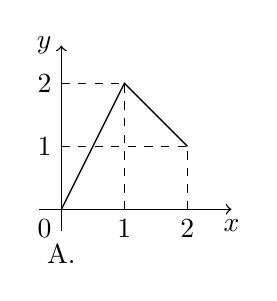
\begin{tikzpicture}[scale=0.8,line width=0.5pt]
\draw[->] (-0.35,0)--(2.7,0) node[below]{$x$};
\draw[->] (0,-0.35)--(0,2.6) node[left]{$y$};
\draw[dashed] (0,1)--(2,1) (0,2)--(1,2) (1,0)--(1,2) (2,0)--(2,1);
\draw (0,0)--(1,2)--(2,1);
\node[below left] at (0,0) {$0$};
\node[below] at (1,0) {$1$}; \node[below] at (2,0) {$2$};
\node[left] at (0,1) {$1$}; \node[left] at (0,2) {$2$};
\node[anchor=north] at (0,-0.4) {A.};
\end{tikzpicture}
&
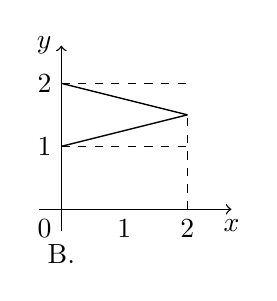
\begin{tikzpicture}[scale=0.8,line width=0.5pt]
\draw[->] (-0.35,0)--(2.7,0) node[below]{$x$};
\draw[->] (0,-0.35)--(0,2.6) node[left]{$y$};
\draw[dashed] (0,1)--(2,1) (0,2)--(2,2) (2,0)--(2,1.5);
\draw (0,2)--(2,1.5);
\draw (0,1)--(2,1.5);
\node[below left] at (0,0) {$0$};
\node[below] at (1,0) {$1$}; \node[below] at (2,0) {$2$};
\node[left] at (0,1) {$1$}; \node[left] at (0,2) {$2$};
\node[anchor=north] at (0,-0.4) {B.};
\end{tikzpicture}
\\[12pt]
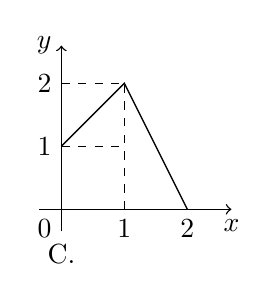
\begin{tikzpicture}[scale=0.8,line width=0.5pt]
\draw[->] (-0.35,0)--(2.7,0) node[below]{$x$};
\draw[->] (0,-0.35)--(0,2.6) node[left]{$y$};
\draw[dashed] (0,1)--(1,1) (0,2)--(1,2) (1,0)--(1,2);
\draw (0,1)--(1,2)--(2,0);
\node[below left] at (0,0) {$0$};
\node[below] at (1,0) {$1$}; \node[below] at (2,0) {$2$};
\node[left] at (0,1) {$1$}; \node[left] at (0,2) {$2$};
\node[anchor=north] at (0,-0.4) {C.};
\end{tikzpicture}
&
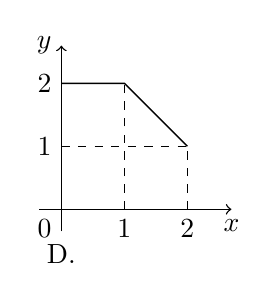
\begin{tikzpicture}[scale=0.8,line width=0.5pt]
\draw[->] (-0.35,0)--(2.7,0) node[below]{$x$};
\draw[->] (0,-0.35)--(0,2.6) node[left]{$y$};
\draw[dashed] (0,1)--(2,1) (1,0)--(1,2) (2,0)--(2,1);
\draw (0,2)--(1,2)--(2,1);
\node[below left] at (0,0) {$0$};
\node[below] at (1,0) {$1$}; \node[below] at (2,0) {$2$};
\node[left] at (0,1) {$1$}; \node[left] at (0,2) {$2$};
\node[anchor=north] at (0,-0.4) {D.};
\end{tikzpicture}
\end{tabular}
\end{center}

\ifanswer
\solbegin
\step{对于 $A$，当 $0\leqslant x\leqslant2$ 时，$0\leqslant y\leqslant2$，故 $A$ 错误；}
\step{对于 $B$，当 $0\leqslant x\leqslant2$ 时，任取一个 $x$ 的值，有两个 $y$ 与之对应，故 $B$ 错误；}
\step{对于 $C$，当 $0\leqslant x\leqslant2$ 时，$0\leqslant y\leqslant2$，故 $C$ 错误；}
\step{对于 $D$，当 $0\leqslant x\leqslant2$ 时，$0\leqslant y\leqslant2$，故 $D$ 正确.}
\step{故选 $D$.}
\solend
\fi

\item 下列函数中与函数 $y=x$ 是同一函数的是\mbox{（\quad）}

\keepwithprev
A. $y=\sqrt{x^2}$\qquad\quad B. $y=(\sqrt x)^2$\qquad\quad C. $u=\dfrac{v^2}{v}$\qquad\quad D. $m=\sqrt[5]{n^5}$

\ifanswer
\solbegin
\step{对于 $A$，$y=\sqrt{x^2}=\lvert x\rvert$，与函数 $y=x$ 的对应关系不相同，不是同一函数；}
\step{对于 $B$，$y=(\sqrt x)^2=x(x\geqslant0)$，与函数 $y=x(x\in\R)$ 的定义域不相同，不是同一函数；}
\step{对于 $C$，$u=\dfrac{v^2}{v}=v(v\neq0)$，与函数 $y=x(x\in\R)$ 的定义域不相同，不是同一函数；}
\step{对于 $D$，$m=\sqrt[5]{n^5}=n(n\in\R)$，与函数 $y=x(x\in\R)$ 的定义域相同，对应关系也相同，是同一函数.}
\step{故选 $D$.}
\solend
\fi

\item 某校高一四班学生 $46$ 人，寒假参加体育训练，其中足球队 $25$ 人，排球队 $22$ 人，游泳队 $24$ 人，足球排球都参加的有 $12$ 人，足球游泳都参加的有 $9$ 人，排球游泳都参加的有 $8$ 人，问：三项都参加的学生数为\mbox{（\quad）}

\keepwithprev
A. $2$\qquad\qquad B. $3$\qquad\qquad C. $4$\qquad\qquad D. $5$

\ifanswer
\solbegin
\step{设集合 $A=\{$参加足球队的学生$\}$，集合 $B=\{$参加排球队的学生$\}$，}
\step{集合 $C=\{$参加游泳队的学生$\}$，}
\step{则 $\operatorname{card}(A)=25$，$\operatorname{card}(B)=22$，$\operatorname{card}(C)=24$，}
\step{$\operatorname{card}(A\cap B)=12$，$\operatorname{card}(A\cap C)=9$，$\operatorname{card}(B\cap C)=8$，}
\step{设三项都参加的有 $x$ 人，即 $\operatorname{card}(A\cap B\cap C)=x$，$\operatorname{card}(A\cup B\cup C)=46$，}
\step{由 $\operatorname{card}(A\cup B\cup C)=\operatorname{card}A+\operatorname{card}B+\operatorname{card}C-\operatorname{card}(A\cap B)$}
\step{$-\operatorname{card}(B\cap C)-\operatorname{card}(A\cap C)+\operatorname{card}(A\cap B\cap C)$，}
\step{即 $46=25+22+24-12-8-9+x$，解得 $x=4$，所以三项都参加的有 $4$ 人.}
\step{故选 $C$.}
\solend
\fi

\item 已知 $\lg a$、$\lg b$ 是方程 $6x^2-4x-3=0$ 的两根，则 $\left(\lg\dfrac ab\right)^2$ 等于\mbox{（\quad）}

\keepwithprev
A. $\dfrac49$\qquad\qquad B. $\dfrac{13}{9}$\qquad\qquad C. $\dfrac{14}{9}$\qquad\qquad D. $\dfrac{22}{9}$

\ifanswer
\solbegin
\step{由韦达定理得 $\lg a+\lg b=\dfrac23$，$\lg a\cdot\lg b=-\dfrac12$，}
\step{所以 $\left(\lg\dfrac ab\right)^2=(\lg a-\lg b)^2=(\lg a+\lg b)^2-4\lg a\lg b=\dfrac49+2=\dfrac{22}{9}$. 故选 $D$.}
\solend
\fi

\end{enumerate}

\bigsec{三、解答题}

\begin{enumerate}
\setcounter{enumi}{16}

\item （1）用分数指数幂表示 $\sqrt[3]{a^2}\cdot\sqrt{a^3}$；

（2）已知 $a^{\frac12}+a^{-\frac12}=3$，求 $a+a^{-1}$.

\ifanswer
\solbegin
\step{（1）$\sqrt[3]{a^2}\cdot\sqrt{a^3}=a^{\frac23}\times a^{\frac32}=a^{\frac{13}6}$.}
\step{（2）由 $a^{\frac12}+a^{-\frac12}=3$，平方得 $a+2+a^{-1}=9$，故 $a+a^{-1}=7$.}
\solend
\fi

\item 已知 $f(x)=\begin{cases}x,x>0\\-x^2-2x+1,x\leqslant0\end{cases}$.

（1）求 $f(f(-2))$ 的值；

（2）若 $f(x_0)=2$，求 $x_0$ 的值.

\ifanswer
\solbegin
\step{（1）$f(x)=\begin{cases}x,x>0\\-x^2-2x+1,x\leqslant0\end{cases}$，则 $f(-2)=-(-2)^2-2\times(-2)+1=1$，}
\step{则有 $f(f(-2))=f(1)=1$；}
\step{（2）当 $x_0>0$ 时，$f(x_0)=x_0$，又 $f(x_0)=2$，所以 $x_0=2$，}
\step{当 $x_0\leqslant0$ 时，$f(x_0)=-x_0^2-2x_0+1$，又 $f(x_0)=2$，}
\step{所以 $-x_0^2-2x_0+1=2$，故 $x_0=-1$，}
\step{综上，$x_0$ 的值为 $-1$ 或 $2$.}
\solend
\fi

\item 已知集合 $A=\{x\mid\lvert 1+x\rvert+\lvert x\rvert<5\}$，$B=\left\{x\,\middle\vert\,\dfrac2{x-m}\geqslant1\right\}$，$p:x\in A$，$q:x\in B$.

（1）若 $m=0$，且 $p$ 真 $q$ 假，求实数 $x$ 的取值范围；

（2）若 $q$ 是 $p$ 的充分不必要条件，求实数 $m$ 的取值范围.

\ifanswer
\solbegin
\step{（1）当 $x\geqslant0$ 时，不等式 $\lvert 1+x\rvert+\lvert x\rvert<5$ 化为 $1+x+x<5$，解得 $0\leqslant x<2$；}
\step{当 $-1\leqslant x<0$ 时，不等式 $\lvert 1+x\rvert+\lvert x\rvert<5$ 化为 $1+x-x<5$ 恒成立，}
\step{故 $-1\leqslant x<0$；}
\step{当 $x<-1$ 时，不等式 $\lvert 1+x\rvert+\lvert x\rvert<5$ 化为 $-1-x-x<5$，}
\step{解得 $-3<x<-1$.}
\step{综上所述，$\lvert 1+x\rvert+\lvert x\rvert<5$ 等价于 $-3<x<2$，}
\step{所以 $\lvert 1+x\rvert+\lvert x\rvert<5$ 的解集为 $A=(-3,2)$，}
\step{若 $m=0$，则 $B=\left\{x\,\middle\vert\,\dfrac2x\geqslant1\right\}=\{x\mid 0<x\leqslant2\}$，得 $\overline{B}=(-\infty,0]\cup(2,+\infty)$，}
\step{由 $p$ 真 $q$ 假，得 $x\in(A\cap\overline{B})=(-3,0]$，即 $x$ 的取值范围为 $(-3,0]$；}
\step{（2）由 $\dfrac2{x-m}\geqslant1$，得 $\begin{cases}x-m>0\\x-m\leqslant2\end{cases}$，解得 $m<x\leqslant m+2$，}
\step{所以 $B=\left\{x\,\middle\vert\,\dfrac2{x-m}\geqslant1\right\}=(m,m+2]$，}
\step{由（1）的结论，得 $A=(-3,2)$，}
\step{若 $q$ 是 $p$ 的充分不必要条件，则 $B$ 是 $A$ 的真子集，得 $\begin{cases}m\geqslant-3\\m+2<2\end{cases}$，}
\step{解得 $-3\leqslant m<0$，即实数 $m$ 的取值范围是 $[-3,0)$.}
\solend
\fi

\item 某企业计划在 $2026$ 年布局人工智能大模型应用开发，生产智能终端配套的 $AI$ 算法服务包. 通过市场分析，全年需投入固定成本 $260$ 万元（含研发、服务器部署等），每生产 $x$ 千个算法服务包，需另投入成本 $R(x)$ 万元，且
$R(x)=\begin{cases}10x^2+100x,0<x\leqslant40\\601x+\dfrac{10000}{x}-7260,x>40\end{cases}$. 已知每个算法服务包的售价为 $0.6$ 万元，假设年内生产的服务包当年能全部销售完.

（1）试写出 $2026$ 年利润 $L$（万元）关于年产量 $x$（千个）的函数解析式；

（2）当 $2026$ 年产量为多少千个时，企业所获利润最大？并求出最大利润.

\ifanswer
\solbegin
\step{（1）$L(x)=x\cdot1000\times0.6-R(x)-260=600x-R(x)-260$，}
\step{当 $0<x\leqslant40$ 时，}
\step{$L(x)=600x-(10x^2+100x)-260=-10x^2+500x-260$；}
\step{当 $x>40$ 时，}
\step{$L(x)=600x-\left(601x+\dfrac{10000}{x}-7260\right)-260=7000-x-\dfrac{10000}{x}$；}
\step{综上，$L(x)=\begin{cases}-10x^2+500x-260,0<x\leqslant40\\7000-x-\dfrac{10000}{x},x>40\end{cases}$；}
\step{（2）当 $0<x\leqslant40$ 时，$L(x)=-10x^2+500x-260=-10(x-25)^2+5990$，}
\step{当 $x=25$ 时，函数 $L(x)$ 有最大值 $5990$；}
\step{当 $x>40$ 时，$L(x)=7000-x-\dfrac{10000}{x}=7000-\left(x+\dfrac{10000}{x}\right)$}
\step{$\leqslant7000-2\sqrt{x\cdot\dfrac{10000}{x}}=7000-2\times100=6800$，}
\step{当且仅当 $x=\dfrac{10000}{x}$ 时取等号，}
\step{所以当 $x=100$ 时，函数 $L(x)$ 有最大值 $6800$；}
\step{因为 $6800>5990$，所以 $2026$ 年产量为 $100$ 千个时，企业所获利润最大，}
\step{最大利润为 $6800$ 万元.}
\solend
\fi

\item 已知二次函数 $f(x)=ax^2+bx+c$.

（1）若 $f(x)>0$ 的解集为 $\{x\mid-3<x<4\}$，解关于 $x$ 的不等式 $bx^2+2ax-(c+3b)<0$；

（2）若函数满足 $f(x+1)-f(x)=2x+2$，且 $f(0)=1$. 求 $f(x)$ 的解析式；

（3）若对任意 $x\in\R$，不等式 $f(x)\geqslant2ax+b$ 恒成立，求 $\dfrac{b^2}{4(a^2+c^2)}$ 的最大值.

\ifanswer
\solbegin
\step{（1）由题意二次函数 $f(x)=ax^2+bx+c$，}
\step{若 $f(x)>0$ 的解集为 $\{x\mid-3<x<4\}$，}
\step{得 $-3$、$4$ 为方程 $ax^2+bx+c=0$ 的根，且 $a<0$，}
\step{则 $\begin{cases}-3+4=-\dfrac ba\\-3\times4=\dfrac ca\end{cases}$，即 $b=-a$，$c=-12a$，}
\step{则不等式 $bx^2+2ax-(c+3b)<0$，即为 $-ax^2+2ax+15a<0(a<0)$，}
\step{则 $x^2-2x-15<0$，解得 $-3<x<5$，}
\step{所以不等式 $bx^2+2ax-(c+3b)<0$ 的解集为 $(-3,5)$；}
\step{（2）由 $f(x)=ax^2+bx+c(a\neq0)$，}
\step{则 $f(x+1)-f(x)=a(x+1)^2+b(x+1)+c-(ax^2+bx+c)=2ax+a+b$，}
\step{又 $f(x+1)-f(x)=2x+2$，故 $\begin{cases}2a=2\\a+b=2\end{cases}$，解得 $a=1$，$b=1$，}
\step{由 $f(0)=1$，得 $c=1$，所以 $f(x)=x^2+x+1$；}
\step{（3）由题意二次函数 $f(x)=ax^2+bx+c$，}
\step{若对任意 $x\in\R$，不等式 $f(x)\geqslant2ax+b$ 恒成立，}
\step{得对任意 $x\in\R$，$ax^2+bx+c\geqslant2ax+b$ 恒成立，}
\step{整理得 $ax^2+(b-2a)x+c-b\geqslant0$ 恒成立，}
\step{因为 $a$ 不为 $0$，所以 $\begin{cases}a>0\\\Delta=(b-2a)^2-4a(c-b)\leqslant0\end{cases}$，}
\step{所以 $0\leqslant b^2\leqslant4a(c-a)$，所以 $\dfrac{b^2}{4(a^2+c^2)}\leqslant\dfrac{ac-a^2}{a^2+c^2}=\dfrac{\frac ca-1}{1+\left(\frac ca\right)^2}$，}
\step{令 $t=\dfrac ca-1$，因为 $0\leqslant b^2\leqslant4a(c-a)$，所以 $c\geqslant a>0\Rightarrow t\geqslant0$，}
\step{若 $t=0$ 时，此时 $\dfrac{b^2}{4(a^2+c^2)}\leqslant\dfrac{\frac ca-1}{1+\left(\frac ca\right)^2}=0$，}
\step{若 $t>0$ 时，$\dfrac{b^2}{4(a^2+c^2)}\leqslant\dfrac{t}{1+(t+1)^2}=\dfrac{t}{t^2+2t+2}=\dfrac1{t+\frac2t+2}$}
\step{$\leqslant\dfrac1{2\sqrt2+2}=\dfrac{\sqrt2-1}{2}$，}
\step{当且仅当 $t=\dfrac2t$，即 $t=\sqrt2$ 时，即 $c=(1+\sqrt2)a$ 时，上式取等号.}
\step{综上所述，$\dfrac{b^2}{4(a^2+c^2)}$ 的最大值为 $\dfrac{\sqrt2-1}{2}$.}
\solend
\fi

\end{enumerate}

\end{document}
"
% 紧凑版：xelatex "\def\iscompact{1}% 高一117_陆行中学_期中.tex
%   —— 高一上数学“2026-2027 年陆行中学高一上期中”（试卷版/答案版）
% 试卷版：xelatex 高一117_陆行中学_期中.tex
% 答案版：xelatex "\def\isanswer{1}% 高一117_陆行中学_期中.tex
%   —— 高一上数学“2026-2027 年陆行中学高一上期中”（试卷版/答案版）
% 试卷版：xelatex 高一117_陆行中学_期中.tex
% 答案版：xelatex "\def\isanswer{1}% 高一117_陆行中学_期中.tex
%   —— 高一上数学“2026-2027 年陆行中学高一上期中”（试卷版/答案版）
% 试卷版：xelatex 高一117_陆行中学_期中.tex
% 答案版：xelatex "\def\isanswer{1}\input{高一117_陆行中学_期中.tex}"
% 紧凑版：xelatex "\def\iscompact{1}\input{高一117_陆行中学_期中.tex}"
%
% 原始材料：微信公众号“魔都数学加油站”文章，作者破晓，2026-11-06 17:58 发布；
% 连载“27学年高一117”，原文标题“27学年高一117——2026-2027年上海市陆行中学高一上期中”；
% 原文链接：https://mp.weixin.qq.com/s/of8iPW26dvDyXWohudT0vw。
% 正文为 10 张 PNG 页（第 1、3、4、8、9、10 页 2560×3620，其余 4762×6735），
% 题目下印有【解析】或【答案】，为讲评版。
% 题目、解析均据原图转录；卷面红色水印及公众号页脚未录入。
%
% 卷首标题：原卷印作“2026-2027 年陆行中学高一上期中”（公众号标题中的“上海市”
% 卷面标题行没有，本稿照卷面），年份区间按全稿惯例排 en dash；原卷未印副标题，本稿按题目内容
% 标为“集合与常用逻辑用语、不等式、函数”（期中卷跨三章，含指数／对数与函数，与 112 同）。
%
% 与原卷的排版差异：
%   ① 原文从第 3 题起，填空题 3—12、选择题 13—16、解答题 17—21，共 19 题，本稿保留原题号；
%   ② 原卷每题下直接印【解析】／【答案】，本稿按全稿惯例置于答案版；第 4、6、8 题只印
%      【答案】，另提 \ans{}；其余选择题答案在解析末句“故选 …”，括号内留空；
%   ③ 原卷未印副标题，本稿按“知识模块”口径补出；
%   ④ 原卷填空横线按全稿惯例排为 \blankline[4.4em]；选择题括号排 \mbox{（\quad）}、
%      选项段前按惯例加 \keepwithprev；解答题不留作答区（原卷为讲评版，与 109—116 同）；
%   ⑤ 原卷 $max$／$min$ 排斜体，按 96 成例改 \max／\min；数集 $R$ 按惯例改 \R。
%
% 判别式字形：第 11 题与第 21 题 (3) 的判别式原卷排 $\Delta$（等腰、右厚），照录 \Delta。
%
% 子集符号：第 5 题的 $B\subseteq A$ 印有下划线，照录 \subseteq。
%
% 第 13 题四个坐标图选项按原图形状用 TikZ 重排（三版都出）；原卷另有第 12 题的
%   $a\odot b$ 自定义运算、第 15 题的 $\operatorname{card}$ 记号，均照录。
%
% 原卷存疑照录：第 12 题解析的 $\min\{\left|x\right|\odot\left|3-x\right|\}$ 一行、
%   第 20 题 $R(x)$ 分段函数与 $L(x)$ 的推导，均按原卷印刷行照录。
%   第 20 题题干开头原卷有一段会议背景引语（非数学信息），本稿从“某企业计划在
%   $2026$ 年布局…”起照录题目主体，全部数据、设问与解析均完整保留。
%
% 行数核对：逐题数 \step/\stepm 条数，合计 106 条（Q3：1；Q4：0；Q5：5；Q6：0；Q7：3；
% Q8：0；Q9：3；Q10：3；Q11：5；Q12：6；Q13：5；Q14：5；Q15：9；Q16：2；Q17：2；
% Q18：6；Q19：14；Q20：14；Q21：23），与原卷印刷行逐题相等（cases／TikZ 图块作一个
% 印刷行计）。第 4、6、8 题只印【答案】，提 \ans{}，不计入 \step 账。
%
\documentclass[a4paper,11pt]{article}
\usepackage{common}

\begin{document}

\examtitlest[3]{2026--2027 年陆行中学高一上期中}{集合与常用逻辑用语、不等式、函数}

\bigsec{一、填空题}

\begin{enumerate}
\setcounter{enumi}{2}

\item 已知 $10^a=2$,$10^b=5$，则 $10^{3a-2b}$ 的值为\blankline[4.4em].

\ifanswer
\solbegin
\step{$10^{3a-2b}=\dfrac{10^{3a}}{10^{2b}}=\dfrac{(10^a)^3}{(10^b)^2}=\dfrac{2^3}{5^2}=\dfrac8{25}$.}
\solend
\fi

\item 已知不等式 $\lvert x+1\rvert+\lvert x-3\rvert\geqslant4$ 恒成立，则取等号时 $x$ 的取值范围是\blankline[4.4em].

\ifanswer
\ans{$[-1,3]$}
\fi

\item 集合 $A=\{1,2,a^2\}$，$B=\{2,a\}$，若 $B\subseteq A$，则 $a$ 的值为\blankline[4.4em].

\ifanswer
\solbegin
\step{因为 $B\subseteq A$，所以 $a=1$ 或 $a=a^2$，}
\step{当 $a=1$ 时，$a^2=1$，不满足元素的互异性，故舍去；}
\step{当 $a=a^2$ 时，解得 $a=1$（舍）或 $a=0$，}
\step{当 $a=0$ 时，$A=\{1,2,0\}$，$B=\{2,0\}$，满足题意.}
\step{综上，$a=0$.}
\solend
\fi

\item 若 $x>\dfrac35$，则 $y=5x+\dfrac1{5x-3}$ 的最小值是\blankline[4.4em].

\ifanswer
\ans{$5$}
\fi

\item 已知 $a>0$，$b>0$，且 $a+b=1$，则 $\dfrac3a+\dfrac1b$ 的最小值是\blankline[4.4em].

\ifanswer
\solbegin
\step{$a>0$，$b>0$，且 $a+b=1$，}
\step{$\dfrac3a+\dfrac1b=\left(\dfrac3a+\dfrac1b\right)(a+b)=\dfrac{3b}{a}+\dfrac ab+4\geqslant2\sqrt3+4$，}
\step{当且仅当 $\dfrac{3b}{a}=\dfrac ab$ 时取等号，所以 $\dfrac3a+\dfrac1b$ 的最小值为 $2\sqrt3+4$.}
\solend
\fi

\item 已知 $\log_2 5=a$，则 $\log_5 10=$\blankline[4.4em]（用含 $a$ 的代数式表示）.

\ifanswer
\ans{$1+\dfrac1a$}
\fi

\item 已知 $p:2<x\leqslant3$，$q:\lvert x-a\rvert<2$，若 $p$ 是 $q$ 的充分不必要条件，则实数 $a$ 的取值范围为\blankline[4.4em].

\ifanswer
\solbegin
\step{由 $\lvert x-a\rvert<2$ 得 $a-2<x<a+2$，即 $p:2<x\leqslant3$，$q:a-2<x<a+2$.}
\step{因为 $p$ 是 $q$ 的充分不必要条件，所以 $\begin{cases}a-2\leqslant2\\a+2>3\end{cases}$，解得 $1<a\leqslant4$，}
\step{所以实数 $a$ 的取值范围为 $(1,4]$.}
\solend
\fi

\item 已知 $a>1$,$b>1$，若 $\log_a b+\log_b a=2$，且 $ab=2$，则 $\log_2(a+b)=$\blankline[4.4em].

\ifanswer
\solbegin
\step{由 $\log_a b+\log_b a=2$,$a>1$,$b>1$，得 $\log_a b+\dfrac1{\log_a b}=2$，}
\step{即 $(\log_a b)^2-2\log_a b+1=0$，则 $(\log_a b-1)^2=0$，即 $\log_a b=1$，则 $a=b$，}
\step{又 $ab=2$，则 $a=b=\sqrt2$，所以 $\log_2(a+b)=\log_2(2\sqrt2)=\log_2 2^{\frac32}=\dfrac32$.}
\solend
\fi

\item 已知函数 $f(x)=\sqrt{2kx^2+kx+\dfrac34}$ 的定义域为实数集 $\R$，则实数 $k$ 的取值范围\blankline[4.4em].

\ifanswer
\solbegin
\step{因为函数 $f(x)=\sqrt{2kx^2+kx+\dfrac34}$ 的定义域为实数集 $\R$，}
\step{所以 $2kx^2+kx+\dfrac34\geqslant0$ 在 $\R$ 上恒成立，}
\step{当 $k=0$ 时，$\dfrac34\geqslant0$，恒成立；}
\step{当 $k\neq0$ 时，则有 $\begin{cases}2k>0\\\Delta=k^2-4\times2k\times\dfrac34\leqslant0\end{cases}$，解得 $0<k\leqslant6$；}
\step{综上，实数 $k$ 的取值范围为 $[0,6]$.}
\solend
\fi

\item 对于两个实数 $a$、$b$，定义运算 $a\odot b$ 如下：若 $a\geqslant b$，则 $a\odot b=a$；若 $a<b$，则 $a\odot b=b$. 若 $x$、$y\in\R$，则 $\lvert x-y\rvert\odot\lvert 3-x\rvert\odot\lvert x+y\rvert$ 的最小值是\blankline[4.4em].

\ifanswer
\solbegin
\step{由题意得 $a\odot b=\max\{a,b\}$，所以 $\lvert a+b\rvert\odot\lvert a-b\rvert=\max\{\lvert a+b\rvert,\lvert a-b\rvert\}$，}
\step{设 $\max\{\lvert a+b\rvert,\lvert a-b\rvert\}=M$，则 $\begin{cases}M\geqslant\lvert a+b\rvert\\M\geqslant\lvert a-b\rvert\end{cases}$，}
\step{所以 $2M\geqslant\lvert a+b\rvert+\lvert a-b\rvert\geqslant2\lvert a\rvert$，则 $\lvert a+b\rvert\odot\lvert a-b\rvert\geqslant\lvert a\rvert$，}
\step{所以 $\min\{\lvert x-y\rvert\odot\lvert 3-x\rvert\odot\lvert x+y\rvert\}=\min\{\lvert x-y\rvert\odot\lvert x+y\rvert\odot\lvert 3-x\rvert\}$}
\step{$=\min\{\lvert x\rvert\odot\lvert 3-x\rvert\}=\min\left\{\dfrac32+x\odot\left\lvert\dfrac32-x\right\rvert\right\}=\dfrac32$，}% 原卷该行写法照录
\step{当且仅当 $x=\dfrac32$，$y=0$ 取等号，故 $\lvert x-y\rvert\odot\lvert 3-x\rvert\odot\lvert x+y\rvert$ 的最小值是 $\dfrac32$.}
\solend
\fi

\end{enumerate}

\bigsec{二、选择题}

\begin{enumerate}
\setcounter{enumi}{12}

\item 设 $A=\{x\mid 0\leqslant x\leqslant2\}$，$B=\{y\mid 1\leqslant y\leqslant2\}$，下列图形能表示从集合 $A$ 到集合 $B$ 的函数图像的是\mbox{（\quad）}

\keepwithprev
\begin{center}
% 原卷四个坐标图选项按原图形状用 TikZ 重排。
\begin{tabular}{c@{\qquad\qquad}c}
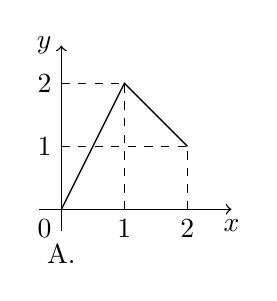
\begin{tikzpicture}[scale=0.8,line width=0.5pt]
\draw[->] (-0.35,0)--(2.7,0) node[below]{$x$};
\draw[->] (0,-0.35)--(0,2.6) node[left]{$y$};
\draw[dashed] (0,1)--(2,1) (0,2)--(1,2) (1,0)--(1,2) (2,0)--(2,1);
\draw (0,0)--(1,2)--(2,1);
\node[below left] at (0,0) {$0$};
\node[below] at (1,0) {$1$}; \node[below] at (2,0) {$2$};
\node[left] at (0,1) {$1$}; \node[left] at (0,2) {$2$};
\node[anchor=north] at (0,-0.4) {A.};
\end{tikzpicture}
&
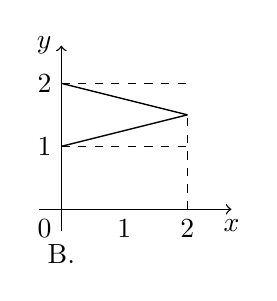
\begin{tikzpicture}[scale=0.8,line width=0.5pt]
\draw[->] (-0.35,0)--(2.7,0) node[below]{$x$};
\draw[->] (0,-0.35)--(0,2.6) node[left]{$y$};
\draw[dashed] (0,1)--(2,1) (0,2)--(2,2) (2,0)--(2,1.5);
\draw (0,2)--(2,1.5);
\draw (0,1)--(2,1.5);
\node[below left] at (0,0) {$0$};
\node[below] at (1,0) {$1$}; \node[below] at (2,0) {$2$};
\node[left] at (0,1) {$1$}; \node[left] at (0,2) {$2$};
\node[anchor=north] at (0,-0.4) {B.};
\end{tikzpicture}
\\[12pt]
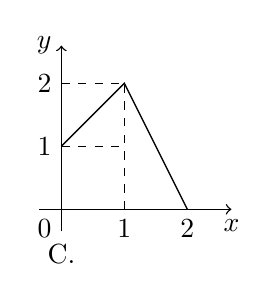
\begin{tikzpicture}[scale=0.8,line width=0.5pt]
\draw[->] (-0.35,0)--(2.7,0) node[below]{$x$};
\draw[->] (0,-0.35)--(0,2.6) node[left]{$y$};
\draw[dashed] (0,1)--(1,1) (0,2)--(1,2) (1,0)--(1,2);
\draw (0,1)--(1,2)--(2,0);
\node[below left] at (0,0) {$0$};
\node[below] at (1,0) {$1$}; \node[below] at (2,0) {$2$};
\node[left] at (0,1) {$1$}; \node[left] at (0,2) {$2$};
\node[anchor=north] at (0,-0.4) {C.};
\end{tikzpicture}
&
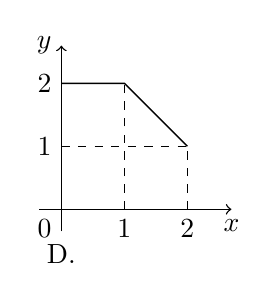
\begin{tikzpicture}[scale=0.8,line width=0.5pt]
\draw[->] (-0.35,0)--(2.7,0) node[below]{$x$};
\draw[->] (0,-0.35)--(0,2.6) node[left]{$y$};
\draw[dashed] (0,1)--(2,1) (1,0)--(1,2) (2,0)--(2,1);
\draw (0,2)--(1,2)--(2,1);
\node[below left] at (0,0) {$0$};
\node[below] at (1,0) {$1$}; \node[below] at (2,0) {$2$};
\node[left] at (0,1) {$1$}; \node[left] at (0,2) {$2$};
\node[anchor=north] at (0,-0.4) {D.};
\end{tikzpicture}
\end{tabular}
\end{center}

\ifanswer
\solbegin
\step{对于 $A$，当 $0\leqslant x\leqslant2$ 时，$0\leqslant y\leqslant2$，故 $A$ 错误；}
\step{对于 $B$，当 $0\leqslant x\leqslant2$ 时，任取一个 $x$ 的值，有两个 $y$ 与之对应，故 $B$ 错误；}
\step{对于 $C$，当 $0\leqslant x\leqslant2$ 时，$0\leqslant y\leqslant2$，故 $C$ 错误；}
\step{对于 $D$，当 $0\leqslant x\leqslant2$ 时，$0\leqslant y\leqslant2$，故 $D$ 正确.}
\step{故选 $D$.}
\solend
\fi

\item 下列函数中与函数 $y=x$ 是同一函数的是\mbox{（\quad）}

\keepwithprev
A. $y=\sqrt{x^2}$\qquad\quad B. $y=(\sqrt x)^2$\qquad\quad C. $u=\dfrac{v^2}{v}$\qquad\quad D. $m=\sqrt[5]{n^5}$

\ifanswer
\solbegin
\step{对于 $A$，$y=\sqrt{x^2}=\lvert x\rvert$，与函数 $y=x$ 的对应关系不相同，不是同一函数；}
\step{对于 $B$，$y=(\sqrt x)^2=x(x\geqslant0)$，与函数 $y=x(x\in\R)$ 的定义域不相同，不是同一函数；}
\step{对于 $C$，$u=\dfrac{v^2}{v}=v(v\neq0)$，与函数 $y=x(x\in\R)$ 的定义域不相同，不是同一函数；}
\step{对于 $D$，$m=\sqrt[5]{n^5}=n(n\in\R)$，与函数 $y=x(x\in\R)$ 的定义域相同，对应关系也相同，是同一函数.}
\step{故选 $D$.}
\solend
\fi

\item 某校高一四班学生 $46$ 人，寒假参加体育训练，其中足球队 $25$ 人，排球队 $22$ 人，游泳队 $24$ 人，足球排球都参加的有 $12$ 人，足球游泳都参加的有 $9$ 人，排球游泳都参加的有 $8$ 人，问：三项都参加的学生数为\mbox{（\quad）}

\keepwithprev
A. $2$\qquad\qquad B. $3$\qquad\qquad C. $4$\qquad\qquad D. $5$

\ifanswer
\solbegin
\step{设集合 $A=\{$参加足球队的学生$\}$，集合 $B=\{$参加排球队的学生$\}$，}
\step{集合 $C=\{$参加游泳队的学生$\}$，}
\step{则 $\operatorname{card}(A)=25$，$\operatorname{card}(B)=22$，$\operatorname{card}(C)=24$，}
\step{$\operatorname{card}(A\cap B)=12$，$\operatorname{card}(A\cap C)=9$，$\operatorname{card}(B\cap C)=8$，}
\step{设三项都参加的有 $x$ 人，即 $\operatorname{card}(A\cap B\cap C)=x$，$\operatorname{card}(A\cup B\cup C)=46$，}
\step{由 $\operatorname{card}(A\cup B\cup C)=\operatorname{card}A+\operatorname{card}B+\operatorname{card}C-\operatorname{card}(A\cap B)$}
\step{$-\operatorname{card}(B\cap C)-\operatorname{card}(A\cap C)+\operatorname{card}(A\cap B\cap C)$，}
\step{即 $46=25+22+24-12-8-9+x$，解得 $x=4$，所以三项都参加的有 $4$ 人.}
\step{故选 $C$.}
\solend
\fi

\item 已知 $\lg a$、$\lg b$ 是方程 $6x^2-4x-3=0$ 的两根，则 $\left(\lg\dfrac ab\right)^2$ 等于\mbox{（\quad）}

\keepwithprev
A. $\dfrac49$\qquad\qquad B. $\dfrac{13}{9}$\qquad\qquad C. $\dfrac{14}{9}$\qquad\qquad D. $\dfrac{22}{9}$

\ifanswer
\solbegin
\step{由韦达定理得 $\lg a+\lg b=\dfrac23$，$\lg a\cdot\lg b=-\dfrac12$，}
\step{所以 $\left(\lg\dfrac ab\right)^2=(\lg a-\lg b)^2=(\lg a+\lg b)^2-4\lg a\lg b=\dfrac49+2=\dfrac{22}{9}$. 故选 $D$.}
\solend
\fi

\end{enumerate}

\bigsec{三、解答题}

\begin{enumerate}
\setcounter{enumi}{16}

\item （1）用分数指数幂表示 $\sqrt[3]{a^2}\cdot\sqrt{a^3}$；

（2）已知 $a^{\frac12}+a^{-\frac12}=3$，求 $a+a^{-1}$.

\ifanswer
\solbegin
\step{（1）$\sqrt[3]{a^2}\cdot\sqrt{a^3}=a^{\frac23}\times a^{\frac32}=a^{\frac{13}6}$.}
\step{（2）由 $a^{\frac12}+a^{-\frac12}=3$，平方得 $a+2+a^{-1}=9$，故 $a+a^{-1}=7$.}
\solend
\fi

\item 已知 $f(x)=\begin{cases}x,x>0\\-x^2-2x+1,x\leqslant0\end{cases}$.

（1）求 $f(f(-2))$ 的值；

（2）若 $f(x_0)=2$，求 $x_0$ 的值.

\ifanswer
\solbegin
\step{（1）$f(x)=\begin{cases}x,x>0\\-x^2-2x+1,x\leqslant0\end{cases}$，则 $f(-2)=-(-2)^2-2\times(-2)+1=1$，}
\step{则有 $f(f(-2))=f(1)=1$；}
\step{（2）当 $x_0>0$ 时，$f(x_0)=x_0$，又 $f(x_0)=2$，所以 $x_0=2$，}
\step{当 $x_0\leqslant0$ 时，$f(x_0)=-x_0^2-2x_0+1$，又 $f(x_0)=2$，}
\step{所以 $-x_0^2-2x_0+1=2$，故 $x_0=-1$，}
\step{综上，$x_0$ 的值为 $-1$ 或 $2$.}
\solend
\fi

\item 已知集合 $A=\{x\mid\lvert 1+x\rvert+\lvert x\rvert<5\}$，$B=\left\{x\,\middle\vert\,\dfrac2{x-m}\geqslant1\right\}$，$p:x\in A$，$q:x\in B$.

（1）若 $m=0$，且 $p$ 真 $q$ 假，求实数 $x$ 的取值范围；

（2）若 $q$ 是 $p$ 的充分不必要条件，求实数 $m$ 的取值范围.

\ifanswer
\solbegin
\step{（1）当 $x\geqslant0$ 时，不等式 $\lvert 1+x\rvert+\lvert x\rvert<5$ 化为 $1+x+x<5$，解得 $0\leqslant x<2$；}
\step{当 $-1\leqslant x<0$ 时，不等式 $\lvert 1+x\rvert+\lvert x\rvert<5$ 化为 $1+x-x<5$ 恒成立，}
\step{故 $-1\leqslant x<0$；}
\step{当 $x<-1$ 时，不等式 $\lvert 1+x\rvert+\lvert x\rvert<5$ 化为 $-1-x-x<5$，}
\step{解得 $-3<x<-1$.}
\step{综上所述，$\lvert 1+x\rvert+\lvert x\rvert<5$ 等价于 $-3<x<2$，}
\step{所以 $\lvert 1+x\rvert+\lvert x\rvert<5$ 的解集为 $A=(-3,2)$，}
\step{若 $m=0$，则 $B=\left\{x\,\middle\vert\,\dfrac2x\geqslant1\right\}=\{x\mid 0<x\leqslant2\}$，得 $\overline{B}=(-\infty,0]\cup(2,+\infty)$，}
\step{由 $p$ 真 $q$ 假，得 $x\in(A\cap\overline{B})=(-3,0]$，即 $x$ 的取值范围为 $(-3,0]$；}
\step{（2）由 $\dfrac2{x-m}\geqslant1$，得 $\begin{cases}x-m>0\\x-m\leqslant2\end{cases}$，解得 $m<x\leqslant m+2$，}
\step{所以 $B=\left\{x\,\middle\vert\,\dfrac2{x-m}\geqslant1\right\}=(m,m+2]$，}
\step{由（1）的结论，得 $A=(-3,2)$，}
\step{若 $q$ 是 $p$ 的充分不必要条件，则 $B$ 是 $A$ 的真子集，得 $\begin{cases}m\geqslant-3\\m+2<2\end{cases}$，}
\step{解得 $-3\leqslant m<0$，即实数 $m$ 的取值范围是 $[-3,0)$.}
\solend
\fi

\item 某企业计划在 $2026$ 年布局人工智能大模型应用开发，生产智能终端配套的 $AI$ 算法服务包. 通过市场分析，全年需投入固定成本 $260$ 万元（含研发、服务器部署等），每生产 $x$ 千个算法服务包，需另投入成本 $R(x)$ 万元，且
$R(x)=\begin{cases}10x^2+100x,0<x\leqslant40\\601x+\dfrac{10000}{x}-7260,x>40\end{cases}$. 已知每个算法服务包的售价为 $0.6$ 万元，假设年内生产的服务包当年能全部销售完.

（1）试写出 $2026$ 年利润 $L$（万元）关于年产量 $x$（千个）的函数解析式；

（2）当 $2026$ 年产量为多少千个时，企业所获利润最大？并求出最大利润.

\ifanswer
\solbegin
\step{（1）$L(x)=x\cdot1000\times0.6-R(x)-260=600x-R(x)-260$，}
\step{当 $0<x\leqslant40$ 时，}
\step{$L(x)=600x-(10x^2+100x)-260=-10x^2+500x-260$；}
\step{当 $x>40$ 时，}
\step{$L(x)=600x-\left(601x+\dfrac{10000}{x}-7260\right)-260=7000-x-\dfrac{10000}{x}$；}
\step{综上，$L(x)=\begin{cases}-10x^2+500x-260,0<x\leqslant40\\7000-x-\dfrac{10000}{x},x>40\end{cases}$；}
\step{（2）当 $0<x\leqslant40$ 时，$L(x)=-10x^2+500x-260=-10(x-25)^2+5990$，}
\step{当 $x=25$ 时，函数 $L(x)$ 有最大值 $5990$；}
\step{当 $x>40$ 时，$L(x)=7000-x-\dfrac{10000}{x}=7000-\left(x+\dfrac{10000}{x}\right)$}
\step{$\leqslant7000-2\sqrt{x\cdot\dfrac{10000}{x}}=7000-2\times100=6800$，}
\step{当且仅当 $x=\dfrac{10000}{x}$ 时取等号，}
\step{所以当 $x=100$ 时，函数 $L(x)$ 有最大值 $6800$；}
\step{因为 $6800>5990$，所以 $2026$ 年产量为 $100$ 千个时，企业所获利润最大，}
\step{最大利润为 $6800$ 万元.}
\solend
\fi

\item 已知二次函数 $f(x)=ax^2+bx+c$.

（1）若 $f(x)>0$ 的解集为 $\{x\mid-3<x<4\}$，解关于 $x$ 的不等式 $bx^2+2ax-(c+3b)<0$；

（2）若函数满足 $f(x+1)-f(x)=2x+2$，且 $f(0)=1$. 求 $f(x)$ 的解析式；

（3）若对任意 $x\in\R$，不等式 $f(x)\geqslant2ax+b$ 恒成立，求 $\dfrac{b^2}{4(a^2+c^2)}$ 的最大值.

\ifanswer
\solbegin
\step{（1）由题意二次函数 $f(x)=ax^2+bx+c$，}
\step{若 $f(x)>0$ 的解集为 $\{x\mid-3<x<4\}$，}
\step{得 $-3$、$4$ 为方程 $ax^2+bx+c=0$ 的根，且 $a<0$，}
\step{则 $\begin{cases}-3+4=-\dfrac ba\\-3\times4=\dfrac ca\end{cases}$，即 $b=-a$，$c=-12a$，}
\step{则不等式 $bx^2+2ax-(c+3b)<0$，即为 $-ax^2+2ax+15a<0(a<0)$，}
\step{则 $x^2-2x-15<0$，解得 $-3<x<5$，}
\step{所以不等式 $bx^2+2ax-(c+3b)<0$ 的解集为 $(-3,5)$；}
\step{（2）由 $f(x)=ax^2+bx+c(a\neq0)$，}
\step{则 $f(x+1)-f(x)=a(x+1)^2+b(x+1)+c-(ax^2+bx+c)=2ax+a+b$，}
\step{又 $f(x+1)-f(x)=2x+2$，故 $\begin{cases}2a=2\\a+b=2\end{cases}$，解得 $a=1$，$b=1$，}
\step{由 $f(0)=1$，得 $c=1$，所以 $f(x)=x^2+x+1$；}
\step{（3）由题意二次函数 $f(x)=ax^2+bx+c$，}
\step{若对任意 $x\in\R$，不等式 $f(x)\geqslant2ax+b$ 恒成立，}
\step{得对任意 $x\in\R$，$ax^2+bx+c\geqslant2ax+b$ 恒成立，}
\step{整理得 $ax^2+(b-2a)x+c-b\geqslant0$ 恒成立，}
\step{因为 $a$ 不为 $0$，所以 $\begin{cases}a>0\\\Delta=(b-2a)^2-4a(c-b)\leqslant0\end{cases}$，}
\step{所以 $0\leqslant b^2\leqslant4a(c-a)$，所以 $\dfrac{b^2}{4(a^2+c^2)}\leqslant\dfrac{ac-a^2}{a^2+c^2}=\dfrac{\frac ca-1}{1+\left(\frac ca\right)^2}$，}
\step{令 $t=\dfrac ca-1$，因为 $0\leqslant b^2\leqslant4a(c-a)$，所以 $c\geqslant a>0\Rightarrow t\geqslant0$，}
\step{若 $t=0$ 时，此时 $\dfrac{b^2}{4(a^2+c^2)}\leqslant\dfrac{\frac ca-1}{1+\left(\frac ca\right)^2}=0$，}
\step{若 $t>0$ 时，$\dfrac{b^2}{4(a^2+c^2)}\leqslant\dfrac{t}{1+(t+1)^2}=\dfrac{t}{t^2+2t+2}=\dfrac1{t+\frac2t+2}$}
\step{$\leqslant\dfrac1{2\sqrt2+2}=\dfrac{\sqrt2-1}{2}$，}
\step{当且仅当 $t=\dfrac2t$，即 $t=\sqrt2$ 时，即 $c=(1+\sqrt2)a$ 时，上式取等号.}
\step{综上所述，$\dfrac{b^2}{4(a^2+c^2)}$ 的最大值为 $\dfrac{\sqrt2-1}{2}$.}
\solend
\fi

\end{enumerate}

\end{document}
"
% 紧凑版：xelatex "\def\iscompact{1}% 高一117_陆行中学_期中.tex
%   —— 高一上数学“2026-2027 年陆行中学高一上期中”（试卷版/答案版）
% 试卷版：xelatex 高一117_陆行中学_期中.tex
% 答案版：xelatex "\def\isanswer{1}\input{高一117_陆行中学_期中.tex}"
% 紧凑版：xelatex "\def\iscompact{1}\input{高一117_陆行中学_期中.tex}"
%
% 原始材料：微信公众号“魔都数学加油站”文章，作者破晓，2026-11-06 17:58 发布；
% 连载“27学年高一117”，原文标题“27学年高一117——2026-2027年上海市陆行中学高一上期中”；
% 原文链接：https://mp.weixin.qq.com/s/of8iPW26dvDyXWohudT0vw。
% 正文为 10 张 PNG 页（第 1、3、4、8、9、10 页 2560×3620，其余 4762×6735），
% 题目下印有【解析】或【答案】，为讲评版。
% 题目、解析均据原图转录；卷面红色水印及公众号页脚未录入。
%
% 卷首标题：原卷印作“2026-2027 年陆行中学高一上期中”（公众号标题中的“上海市”
% 卷面标题行没有，本稿照卷面），年份区间按全稿惯例排 en dash；原卷未印副标题，本稿按题目内容
% 标为“集合与常用逻辑用语、不等式、函数”（期中卷跨三章，含指数／对数与函数，与 112 同）。
%
% 与原卷的排版差异：
%   ① 原文从第 3 题起，填空题 3—12、选择题 13—16、解答题 17—21，共 19 题，本稿保留原题号；
%   ② 原卷每题下直接印【解析】／【答案】，本稿按全稿惯例置于答案版；第 4、6、8 题只印
%      【答案】，另提 \ans{}；其余选择题答案在解析末句“故选 …”，括号内留空；
%   ③ 原卷未印副标题，本稿按“知识模块”口径补出；
%   ④ 原卷填空横线按全稿惯例排为 \blankline[4.4em]；选择题括号排 \mbox{（\quad）}、
%      选项段前按惯例加 \keepwithprev；解答题不留作答区（原卷为讲评版，与 109—116 同）；
%   ⑤ 原卷 $max$／$min$ 排斜体，按 96 成例改 \max／\min；数集 $R$ 按惯例改 \R。
%
% 判别式字形：第 11 题与第 21 题 (3) 的判别式原卷排 $\Delta$（等腰、右厚），照录 \Delta。
%
% 子集符号：第 5 题的 $B\subseteq A$ 印有下划线，照录 \subseteq。
%
% 第 13 题四个坐标图选项按原图形状用 TikZ 重排（三版都出）；原卷另有第 12 题的
%   $a\odot b$ 自定义运算、第 15 题的 $\operatorname{card}$ 记号，均照录。
%
% 原卷存疑照录：第 12 题解析的 $\min\{\left|x\right|\odot\left|3-x\right|\}$ 一行、
%   第 20 题 $R(x)$ 分段函数与 $L(x)$ 的推导，均按原卷印刷行照录。
%   第 20 题题干开头原卷有一段会议背景引语（非数学信息），本稿从“某企业计划在
%   $2026$ 年布局…”起照录题目主体，全部数据、设问与解析均完整保留。
%
% 行数核对：逐题数 \step/\stepm 条数，合计 106 条（Q3：1；Q4：0；Q5：5；Q6：0；Q7：3；
% Q8：0；Q9：3；Q10：3；Q11：5；Q12：6；Q13：5；Q14：5；Q15：9；Q16：2；Q17：2；
% Q18：6；Q19：14；Q20：14；Q21：23），与原卷印刷行逐题相等（cases／TikZ 图块作一个
% 印刷行计）。第 4、6、8 题只印【答案】，提 \ans{}，不计入 \step 账。
%
\documentclass[a4paper,11pt]{article}
\usepackage{common}

\begin{document}

\examtitlest[3]{2026--2027 年陆行中学高一上期中}{集合与常用逻辑用语、不等式、函数}

\bigsec{一、填空题}

\begin{enumerate}
\setcounter{enumi}{2}

\item 已知 $10^a=2$,$10^b=5$，则 $10^{3a-2b}$ 的值为\blankline[4.4em].

\ifanswer
\solbegin
\step{$10^{3a-2b}=\dfrac{10^{3a}}{10^{2b}}=\dfrac{(10^a)^3}{(10^b)^2}=\dfrac{2^3}{5^2}=\dfrac8{25}$.}
\solend
\fi

\item 已知不等式 $\lvert x+1\rvert+\lvert x-3\rvert\geqslant4$ 恒成立，则取等号时 $x$ 的取值范围是\blankline[4.4em].

\ifanswer
\ans{$[-1,3]$}
\fi

\item 集合 $A=\{1,2,a^2\}$，$B=\{2,a\}$，若 $B\subseteq A$，则 $a$ 的值为\blankline[4.4em].

\ifanswer
\solbegin
\step{因为 $B\subseteq A$，所以 $a=1$ 或 $a=a^2$，}
\step{当 $a=1$ 时，$a^2=1$，不满足元素的互异性，故舍去；}
\step{当 $a=a^2$ 时，解得 $a=1$（舍）或 $a=0$，}
\step{当 $a=0$ 时，$A=\{1,2,0\}$，$B=\{2,0\}$，满足题意.}
\step{综上，$a=0$.}
\solend
\fi

\item 若 $x>\dfrac35$，则 $y=5x+\dfrac1{5x-3}$ 的最小值是\blankline[4.4em].

\ifanswer
\ans{$5$}
\fi

\item 已知 $a>0$，$b>0$，且 $a+b=1$，则 $\dfrac3a+\dfrac1b$ 的最小值是\blankline[4.4em].

\ifanswer
\solbegin
\step{$a>0$，$b>0$，且 $a+b=1$，}
\step{$\dfrac3a+\dfrac1b=\left(\dfrac3a+\dfrac1b\right)(a+b)=\dfrac{3b}{a}+\dfrac ab+4\geqslant2\sqrt3+4$，}
\step{当且仅当 $\dfrac{3b}{a}=\dfrac ab$ 时取等号，所以 $\dfrac3a+\dfrac1b$ 的最小值为 $2\sqrt3+4$.}
\solend
\fi

\item 已知 $\log_2 5=a$，则 $\log_5 10=$\blankline[4.4em]（用含 $a$ 的代数式表示）.

\ifanswer
\ans{$1+\dfrac1a$}
\fi

\item 已知 $p:2<x\leqslant3$，$q:\lvert x-a\rvert<2$，若 $p$ 是 $q$ 的充分不必要条件，则实数 $a$ 的取值范围为\blankline[4.4em].

\ifanswer
\solbegin
\step{由 $\lvert x-a\rvert<2$ 得 $a-2<x<a+2$，即 $p:2<x\leqslant3$，$q:a-2<x<a+2$.}
\step{因为 $p$ 是 $q$ 的充分不必要条件，所以 $\begin{cases}a-2\leqslant2\\a+2>3\end{cases}$，解得 $1<a\leqslant4$，}
\step{所以实数 $a$ 的取值范围为 $(1,4]$.}
\solend
\fi

\item 已知 $a>1$,$b>1$，若 $\log_a b+\log_b a=2$，且 $ab=2$，则 $\log_2(a+b)=$\blankline[4.4em].

\ifanswer
\solbegin
\step{由 $\log_a b+\log_b a=2$,$a>1$,$b>1$，得 $\log_a b+\dfrac1{\log_a b}=2$，}
\step{即 $(\log_a b)^2-2\log_a b+1=0$，则 $(\log_a b-1)^2=0$，即 $\log_a b=1$，则 $a=b$，}
\step{又 $ab=2$，则 $a=b=\sqrt2$，所以 $\log_2(a+b)=\log_2(2\sqrt2)=\log_2 2^{\frac32}=\dfrac32$.}
\solend
\fi

\item 已知函数 $f(x)=\sqrt{2kx^2+kx+\dfrac34}$ 的定义域为实数集 $\R$，则实数 $k$ 的取值范围\blankline[4.4em].

\ifanswer
\solbegin
\step{因为函数 $f(x)=\sqrt{2kx^2+kx+\dfrac34}$ 的定义域为实数集 $\R$，}
\step{所以 $2kx^2+kx+\dfrac34\geqslant0$ 在 $\R$ 上恒成立，}
\step{当 $k=0$ 时，$\dfrac34\geqslant0$，恒成立；}
\step{当 $k\neq0$ 时，则有 $\begin{cases}2k>0\\\Delta=k^2-4\times2k\times\dfrac34\leqslant0\end{cases}$，解得 $0<k\leqslant6$；}
\step{综上，实数 $k$ 的取值范围为 $[0,6]$.}
\solend
\fi

\item 对于两个实数 $a$、$b$，定义运算 $a\odot b$ 如下：若 $a\geqslant b$，则 $a\odot b=a$；若 $a<b$，则 $a\odot b=b$. 若 $x$、$y\in\R$，则 $\lvert x-y\rvert\odot\lvert 3-x\rvert\odot\lvert x+y\rvert$ 的最小值是\blankline[4.4em].

\ifanswer
\solbegin
\step{由题意得 $a\odot b=\max\{a,b\}$，所以 $\lvert a+b\rvert\odot\lvert a-b\rvert=\max\{\lvert a+b\rvert,\lvert a-b\rvert\}$，}
\step{设 $\max\{\lvert a+b\rvert,\lvert a-b\rvert\}=M$，则 $\begin{cases}M\geqslant\lvert a+b\rvert\\M\geqslant\lvert a-b\rvert\end{cases}$，}
\step{所以 $2M\geqslant\lvert a+b\rvert+\lvert a-b\rvert\geqslant2\lvert a\rvert$，则 $\lvert a+b\rvert\odot\lvert a-b\rvert\geqslant\lvert a\rvert$，}
\step{所以 $\min\{\lvert x-y\rvert\odot\lvert 3-x\rvert\odot\lvert x+y\rvert\}=\min\{\lvert x-y\rvert\odot\lvert x+y\rvert\odot\lvert 3-x\rvert\}$}
\step{$=\min\{\lvert x\rvert\odot\lvert 3-x\rvert\}=\min\left\{\dfrac32+x\odot\left\lvert\dfrac32-x\right\rvert\right\}=\dfrac32$，}% 原卷该行写法照录
\step{当且仅当 $x=\dfrac32$，$y=0$ 取等号，故 $\lvert x-y\rvert\odot\lvert 3-x\rvert\odot\lvert x+y\rvert$ 的最小值是 $\dfrac32$.}
\solend
\fi

\end{enumerate}

\bigsec{二、选择题}

\begin{enumerate}
\setcounter{enumi}{12}

\item 设 $A=\{x\mid 0\leqslant x\leqslant2\}$，$B=\{y\mid 1\leqslant y\leqslant2\}$，下列图形能表示从集合 $A$ 到集合 $B$ 的函数图像的是\mbox{（\quad）}

\keepwithprev
\begin{center}
% 原卷四个坐标图选项按原图形状用 TikZ 重排。
\begin{tabular}{c@{\qquad\qquad}c}
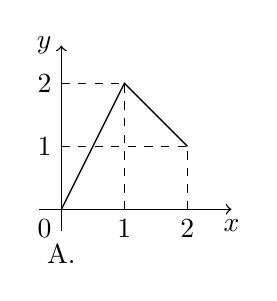
\begin{tikzpicture}[scale=0.8,line width=0.5pt]
\draw[->] (-0.35,0)--(2.7,0) node[below]{$x$};
\draw[->] (0,-0.35)--(0,2.6) node[left]{$y$};
\draw[dashed] (0,1)--(2,1) (0,2)--(1,2) (1,0)--(1,2) (2,0)--(2,1);
\draw (0,0)--(1,2)--(2,1);
\node[below left] at (0,0) {$0$};
\node[below] at (1,0) {$1$}; \node[below] at (2,0) {$2$};
\node[left] at (0,1) {$1$}; \node[left] at (0,2) {$2$};
\node[anchor=north] at (0,-0.4) {A.};
\end{tikzpicture}
&
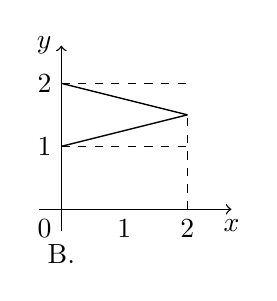
\begin{tikzpicture}[scale=0.8,line width=0.5pt]
\draw[->] (-0.35,0)--(2.7,0) node[below]{$x$};
\draw[->] (0,-0.35)--(0,2.6) node[left]{$y$};
\draw[dashed] (0,1)--(2,1) (0,2)--(2,2) (2,0)--(2,1.5);
\draw (0,2)--(2,1.5);
\draw (0,1)--(2,1.5);
\node[below left] at (0,0) {$0$};
\node[below] at (1,0) {$1$}; \node[below] at (2,0) {$2$};
\node[left] at (0,1) {$1$}; \node[left] at (0,2) {$2$};
\node[anchor=north] at (0,-0.4) {B.};
\end{tikzpicture}
\\[12pt]
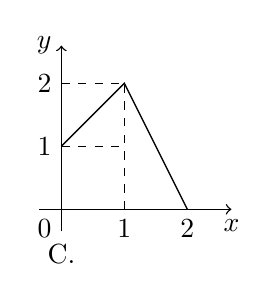
\begin{tikzpicture}[scale=0.8,line width=0.5pt]
\draw[->] (-0.35,0)--(2.7,0) node[below]{$x$};
\draw[->] (0,-0.35)--(0,2.6) node[left]{$y$};
\draw[dashed] (0,1)--(1,1) (0,2)--(1,2) (1,0)--(1,2);
\draw (0,1)--(1,2)--(2,0);
\node[below left] at (0,0) {$0$};
\node[below] at (1,0) {$1$}; \node[below] at (2,0) {$2$};
\node[left] at (0,1) {$1$}; \node[left] at (0,2) {$2$};
\node[anchor=north] at (0,-0.4) {C.};
\end{tikzpicture}
&
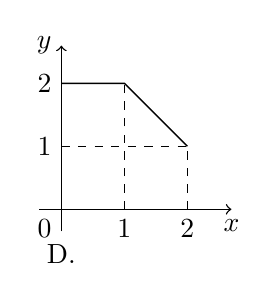
\begin{tikzpicture}[scale=0.8,line width=0.5pt]
\draw[->] (-0.35,0)--(2.7,0) node[below]{$x$};
\draw[->] (0,-0.35)--(0,2.6) node[left]{$y$};
\draw[dashed] (0,1)--(2,1) (1,0)--(1,2) (2,0)--(2,1);
\draw (0,2)--(1,2)--(2,1);
\node[below left] at (0,0) {$0$};
\node[below] at (1,0) {$1$}; \node[below] at (2,0) {$2$};
\node[left] at (0,1) {$1$}; \node[left] at (0,2) {$2$};
\node[anchor=north] at (0,-0.4) {D.};
\end{tikzpicture}
\end{tabular}
\end{center}

\ifanswer
\solbegin
\step{对于 $A$，当 $0\leqslant x\leqslant2$ 时，$0\leqslant y\leqslant2$，故 $A$ 错误；}
\step{对于 $B$，当 $0\leqslant x\leqslant2$ 时，任取一个 $x$ 的值，有两个 $y$ 与之对应，故 $B$ 错误；}
\step{对于 $C$，当 $0\leqslant x\leqslant2$ 时，$0\leqslant y\leqslant2$，故 $C$ 错误；}
\step{对于 $D$，当 $0\leqslant x\leqslant2$ 时，$0\leqslant y\leqslant2$，故 $D$ 正确.}
\step{故选 $D$.}
\solend
\fi

\item 下列函数中与函数 $y=x$ 是同一函数的是\mbox{（\quad）}

\keepwithprev
A. $y=\sqrt{x^2}$\qquad\quad B. $y=(\sqrt x)^2$\qquad\quad C. $u=\dfrac{v^2}{v}$\qquad\quad D. $m=\sqrt[5]{n^5}$

\ifanswer
\solbegin
\step{对于 $A$，$y=\sqrt{x^2}=\lvert x\rvert$，与函数 $y=x$ 的对应关系不相同，不是同一函数；}
\step{对于 $B$，$y=(\sqrt x)^2=x(x\geqslant0)$，与函数 $y=x(x\in\R)$ 的定义域不相同，不是同一函数；}
\step{对于 $C$，$u=\dfrac{v^2}{v}=v(v\neq0)$，与函数 $y=x(x\in\R)$ 的定义域不相同，不是同一函数；}
\step{对于 $D$，$m=\sqrt[5]{n^5}=n(n\in\R)$，与函数 $y=x(x\in\R)$ 的定义域相同，对应关系也相同，是同一函数.}
\step{故选 $D$.}
\solend
\fi

\item 某校高一四班学生 $46$ 人，寒假参加体育训练，其中足球队 $25$ 人，排球队 $22$ 人，游泳队 $24$ 人，足球排球都参加的有 $12$ 人，足球游泳都参加的有 $9$ 人，排球游泳都参加的有 $8$ 人，问：三项都参加的学生数为\mbox{（\quad）}

\keepwithprev
A. $2$\qquad\qquad B. $3$\qquad\qquad C. $4$\qquad\qquad D. $5$

\ifanswer
\solbegin
\step{设集合 $A=\{$参加足球队的学生$\}$，集合 $B=\{$参加排球队的学生$\}$，}
\step{集合 $C=\{$参加游泳队的学生$\}$，}
\step{则 $\operatorname{card}(A)=25$，$\operatorname{card}(B)=22$，$\operatorname{card}(C)=24$，}
\step{$\operatorname{card}(A\cap B)=12$，$\operatorname{card}(A\cap C)=9$，$\operatorname{card}(B\cap C)=8$，}
\step{设三项都参加的有 $x$ 人，即 $\operatorname{card}(A\cap B\cap C)=x$，$\operatorname{card}(A\cup B\cup C)=46$，}
\step{由 $\operatorname{card}(A\cup B\cup C)=\operatorname{card}A+\operatorname{card}B+\operatorname{card}C-\operatorname{card}(A\cap B)$}
\step{$-\operatorname{card}(B\cap C)-\operatorname{card}(A\cap C)+\operatorname{card}(A\cap B\cap C)$，}
\step{即 $46=25+22+24-12-8-9+x$，解得 $x=4$，所以三项都参加的有 $4$ 人.}
\step{故选 $C$.}
\solend
\fi

\item 已知 $\lg a$、$\lg b$ 是方程 $6x^2-4x-3=0$ 的两根，则 $\left(\lg\dfrac ab\right)^2$ 等于\mbox{（\quad）}

\keepwithprev
A. $\dfrac49$\qquad\qquad B. $\dfrac{13}{9}$\qquad\qquad C. $\dfrac{14}{9}$\qquad\qquad D. $\dfrac{22}{9}$

\ifanswer
\solbegin
\step{由韦达定理得 $\lg a+\lg b=\dfrac23$，$\lg a\cdot\lg b=-\dfrac12$，}
\step{所以 $\left(\lg\dfrac ab\right)^2=(\lg a-\lg b)^2=(\lg a+\lg b)^2-4\lg a\lg b=\dfrac49+2=\dfrac{22}{9}$. 故选 $D$.}
\solend
\fi

\end{enumerate}

\bigsec{三、解答题}

\begin{enumerate}
\setcounter{enumi}{16}

\item （1）用分数指数幂表示 $\sqrt[3]{a^2}\cdot\sqrt{a^3}$；

（2）已知 $a^{\frac12}+a^{-\frac12}=3$，求 $a+a^{-1}$.

\ifanswer
\solbegin
\step{（1）$\sqrt[3]{a^2}\cdot\sqrt{a^3}=a^{\frac23}\times a^{\frac32}=a^{\frac{13}6}$.}
\step{（2）由 $a^{\frac12}+a^{-\frac12}=3$，平方得 $a+2+a^{-1}=9$，故 $a+a^{-1}=7$.}
\solend
\fi

\item 已知 $f(x)=\begin{cases}x,x>0\\-x^2-2x+1,x\leqslant0\end{cases}$.

（1）求 $f(f(-2))$ 的值；

（2）若 $f(x_0)=2$，求 $x_0$ 的值.

\ifanswer
\solbegin
\step{（1）$f(x)=\begin{cases}x,x>0\\-x^2-2x+1,x\leqslant0\end{cases}$，则 $f(-2)=-(-2)^2-2\times(-2)+1=1$，}
\step{则有 $f(f(-2))=f(1)=1$；}
\step{（2）当 $x_0>0$ 时，$f(x_0)=x_0$，又 $f(x_0)=2$，所以 $x_0=2$，}
\step{当 $x_0\leqslant0$ 时，$f(x_0)=-x_0^2-2x_0+1$，又 $f(x_0)=2$，}
\step{所以 $-x_0^2-2x_0+1=2$，故 $x_0=-1$，}
\step{综上，$x_0$ 的值为 $-1$ 或 $2$.}
\solend
\fi

\item 已知集合 $A=\{x\mid\lvert 1+x\rvert+\lvert x\rvert<5\}$，$B=\left\{x\,\middle\vert\,\dfrac2{x-m}\geqslant1\right\}$，$p:x\in A$，$q:x\in B$.

（1）若 $m=0$，且 $p$ 真 $q$ 假，求实数 $x$ 的取值范围；

（2）若 $q$ 是 $p$ 的充分不必要条件，求实数 $m$ 的取值范围.

\ifanswer
\solbegin
\step{（1）当 $x\geqslant0$ 时，不等式 $\lvert 1+x\rvert+\lvert x\rvert<5$ 化为 $1+x+x<5$，解得 $0\leqslant x<2$；}
\step{当 $-1\leqslant x<0$ 时，不等式 $\lvert 1+x\rvert+\lvert x\rvert<5$ 化为 $1+x-x<5$ 恒成立，}
\step{故 $-1\leqslant x<0$；}
\step{当 $x<-1$ 时，不等式 $\lvert 1+x\rvert+\lvert x\rvert<5$ 化为 $-1-x-x<5$，}
\step{解得 $-3<x<-1$.}
\step{综上所述，$\lvert 1+x\rvert+\lvert x\rvert<5$ 等价于 $-3<x<2$，}
\step{所以 $\lvert 1+x\rvert+\lvert x\rvert<5$ 的解集为 $A=(-3,2)$，}
\step{若 $m=0$，则 $B=\left\{x\,\middle\vert\,\dfrac2x\geqslant1\right\}=\{x\mid 0<x\leqslant2\}$，得 $\overline{B}=(-\infty,0]\cup(2,+\infty)$，}
\step{由 $p$ 真 $q$ 假，得 $x\in(A\cap\overline{B})=(-3,0]$，即 $x$ 的取值范围为 $(-3,0]$；}
\step{（2）由 $\dfrac2{x-m}\geqslant1$，得 $\begin{cases}x-m>0\\x-m\leqslant2\end{cases}$，解得 $m<x\leqslant m+2$，}
\step{所以 $B=\left\{x\,\middle\vert\,\dfrac2{x-m}\geqslant1\right\}=(m,m+2]$，}
\step{由（1）的结论，得 $A=(-3,2)$，}
\step{若 $q$ 是 $p$ 的充分不必要条件，则 $B$ 是 $A$ 的真子集，得 $\begin{cases}m\geqslant-3\\m+2<2\end{cases}$，}
\step{解得 $-3\leqslant m<0$，即实数 $m$ 的取值范围是 $[-3,0)$.}
\solend
\fi

\item 某企业计划在 $2026$ 年布局人工智能大模型应用开发，生产智能终端配套的 $AI$ 算法服务包. 通过市场分析，全年需投入固定成本 $260$ 万元（含研发、服务器部署等），每生产 $x$ 千个算法服务包，需另投入成本 $R(x)$ 万元，且
$R(x)=\begin{cases}10x^2+100x,0<x\leqslant40\\601x+\dfrac{10000}{x}-7260,x>40\end{cases}$. 已知每个算法服务包的售价为 $0.6$ 万元，假设年内生产的服务包当年能全部销售完.

（1）试写出 $2026$ 年利润 $L$（万元）关于年产量 $x$（千个）的函数解析式；

（2）当 $2026$ 年产量为多少千个时，企业所获利润最大？并求出最大利润.

\ifanswer
\solbegin
\step{（1）$L(x)=x\cdot1000\times0.6-R(x)-260=600x-R(x)-260$，}
\step{当 $0<x\leqslant40$ 时，}
\step{$L(x)=600x-(10x^2+100x)-260=-10x^2+500x-260$；}
\step{当 $x>40$ 时，}
\step{$L(x)=600x-\left(601x+\dfrac{10000}{x}-7260\right)-260=7000-x-\dfrac{10000}{x}$；}
\step{综上，$L(x)=\begin{cases}-10x^2+500x-260,0<x\leqslant40\\7000-x-\dfrac{10000}{x},x>40\end{cases}$；}
\step{（2）当 $0<x\leqslant40$ 时，$L(x)=-10x^2+500x-260=-10(x-25)^2+5990$，}
\step{当 $x=25$ 时，函数 $L(x)$ 有最大值 $5990$；}
\step{当 $x>40$ 时，$L(x)=7000-x-\dfrac{10000}{x}=7000-\left(x+\dfrac{10000}{x}\right)$}
\step{$\leqslant7000-2\sqrt{x\cdot\dfrac{10000}{x}}=7000-2\times100=6800$，}
\step{当且仅当 $x=\dfrac{10000}{x}$ 时取等号，}
\step{所以当 $x=100$ 时，函数 $L(x)$ 有最大值 $6800$；}
\step{因为 $6800>5990$，所以 $2026$ 年产量为 $100$ 千个时，企业所获利润最大，}
\step{最大利润为 $6800$ 万元.}
\solend
\fi

\item 已知二次函数 $f(x)=ax^2+bx+c$.

（1）若 $f(x)>0$ 的解集为 $\{x\mid-3<x<4\}$，解关于 $x$ 的不等式 $bx^2+2ax-(c+3b)<0$；

（2）若函数满足 $f(x+1)-f(x)=2x+2$，且 $f(0)=1$. 求 $f(x)$ 的解析式；

（3）若对任意 $x\in\R$，不等式 $f(x)\geqslant2ax+b$ 恒成立，求 $\dfrac{b^2}{4(a^2+c^2)}$ 的最大值.

\ifanswer
\solbegin
\step{（1）由题意二次函数 $f(x)=ax^2+bx+c$，}
\step{若 $f(x)>0$ 的解集为 $\{x\mid-3<x<4\}$，}
\step{得 $-3$、$4$ 为方程 $ax^2+bx+c=0$ 的根，且 $a<0$，}
\step{则 $\begin{cases}-3+4=-\dfrac ba\\-3\times4=\dfrac ca\end{cases}$，即 $b=-a$，$c=-12a$，}
\step{则不等式 $bx^2+2ax-(c+3b)<0$，即为 $-ax^2+2ax+15a<0(a<0)$，}
\step{则 $x^2-2x-15<0$，解得 $-3<x<5$，}
\step{所以不等式 $bx^2+2ax-(c+3b)<0$ 的解集为 $(-3,5)$；}
\step{（2）由 $f(x)=ax^2+bx+c(a\neq0)$，}
\step{则 $f(x+1)-f(x)=a(x+1)^2+b(x+1)+c-(ax^2+bx+c)=2ax+a+b$，}
\step{又 $f(x+1)-f(x)=2x+2$，故 $\begin{cases}2a=2\\a+b=2\end{cases}$，解得 $a=1$，$b=1$，}
\step{由 $f(0)=1$，得 $c=1$，所以 $f(x)=x^2+x+1$；}
\step{（3）由题意二次函数 $f(x)=ax^2+bx+c$，}
\step{若对任意 $x\in\R$，不等式 $f(x)\geqslant2ax+b$ 恒成立，}
\step{得对任意 $x\in\R$，$ax^2+bx+c\geqslant2ax+b$ 恒成立，}
\step{整理得 $ax^2+(b-2a)x+c-b\geqslant0$ 恒成立，}
\step{因为 $a$ 不为 $0$，所以 $\begin{cases}a>0\\\Delta=(b-2a)^2-4a(c-b)\leqslant0\end{cases}$，}
\step{所以 $0\leqslant b^2\leqslant4a(c-a)$，所以 $\dfrac{b^2}{4(a^2+c^2)}\leqslant\dfrac{ac-a^2}{a^2+c^2}=\dfrac{\frac ca-1}{1+\left(\frac ca\right)^2}$，}
\step{令 $t=\dfrac ca-1$，因为 $0\leqslant b^2\leqslant4a(c-a)$，所以 $c\geqslant a>0\Rightarrow t\geqslant0$，}
\step{若 $t=0$ 时，此时 $\dfrac{b^2}{4(a^2+c^2)}\leqslant\dfrac{\frac ca-1}{1+\left(\frac ca\right)^2}=0$，}
\step{若 $t>0$ 时，$\dfrac{b^2}{4(a^2+c^2)}\leqslant\dfrac{t}{1+(t+1)^2}=\dfrac{t}{t^2+2t+2}=\dfrac1{t+\frac2t+2}$}
\step{$\leqslant\dfrac1{2\sqrt2+2}=\dfrac{\sqrt2-1}{2}$，}
\step{当且仅当 $t=\dfrac2t$，即 $t=\sqrt2$ 时，即 $c=(1+\sqrt2)a$ 时，上式取等号.}
\step{综上所述，$\dfrac{b^2}{4(a^2+c^2)}$ 的最大值为 $\dfrac{\sqrt2-1}{2}$.}
\solend
\fi

\end{enumerate}

\end{document}
"
%
% 原始材料：微信公众号“魔都数学加油站”文章，作者破晓，2026-11-06 17:58 发布；
% 连载“27学年高一117”，原文标题“27学年高一117——2026-2027年上海市陆行中学高一上期中”；
% 原文链接：https://mp.weixin.qq.com/s/of8iPW26dvDyXWohudT0vw。
% 正文为 10 张 PNG 页（第 1、3、4、8、9、10 页 2560×3620，其余 4762×6735），
% 题目下印有【解析】或【答案】，为讲评版。
% 题目、解析均据原图转录；卷面红色水印及公众号页脚未录入。
%
% 卷首标题：原卷印作“2026-2027 年陆行中学高一上期中”（公众号标题中的“上海市”
% 卷面标题行没有，本稿照卷面），年份区间按全稿惯例排 en dash；原卷未印副标题，本稿按题目内容
% 标为“集合与常用逻辑用语、不等式、函数”（期中卷跨三章，含指数／对数与函数，与 112 同）。
%
% 与原卷的排版差异：
%   ① 原文从第 3 题起，填空题 3—12、选择题 13—16、解答题 17—21，共 19 题，本稿保留原题号；
%   ② 原卷每题下直接印【解析】／【答案】，本稿按全稿惯例置于答案版；第 4、6、8 题只印
%      【答案】，另提 \ans{}；其余选择题答案在解析末句“故选 …”，括号内留空；
%   ③ 原卷未印副标题，本稿按“知识模块”口径补出；
%   ④ 原卷填空横线按全稿惯例排为 \blankline[4.4em]；选择题括号排 \mbox{（\quad）}、
%      选项段前按惯例加 \keepwithprev；解答题不留作答区（原卷为讲评版，与 109—116 同）；
%   ⑤ 原卷 $max$／$min$ 排斜体，按 96 成例改 \max／\min；数集 $R$ 按惯例改 \R。
%
% 判别式字形：第 11 题与第 21 题 (3) 的判别式原卷排 $\Delta$（等腰、右厚），照录 \Delta。
%
% 子集符号：第 5 题的 $B\subseteq A$ 印有下划线，照录 \subseteq。
%
% 第 13 题四个坐标图选项按原图形状用 TikZ 重排（三版都出）；原卷另有第 12 题的
%   $a\odot b$ 自定义运算、第 15 题的 $\operatorname{card}$ 记号，均照录。
%
% 原卷存疑照录：第 12 题解析的 $\min\{\left|x\right|\odot\left|3-x\right|\}$ 一行、
%   第 20 题 $R(x)$ 分段函数与 $L(x)$ 的推导，均按原卷印刷行照录。
%   第 20 题题干开头原卷有一段会议背景引语（非数学信息），本稿从“某企业计划在
%   $2026$ 年布局…”起照录题目主体，全部数据、设问与解析均完整保留。
%
% 行数核对：逐题数 \step/\stepm 条数，合计 106 条（Q3：1；Q4：0；Q5：5；Q6：0；Q7：3；
% Q8：0；Q9：3；Q10：3；Q11：5；Q12：6；Q13：5；Q14：5；Q15：9；Q16：2；Q17：2；
% Q18：6；Q19：14；Q20：14；Q21：23），与原卷印刷行逐题相等（cases／TikZ 图块作一个
% 印刷行计）。第 4、6、8 题只印【答案】，提 \ans{}，不计入 \step 账。
%
\documentclass[a4paper,11pt]{article}
\usepackage{common}

\begin{document}

\examtitlest[3]{2026--2027 年陆行中学高一上期中}{集合与常用逻辑用语、不等式、函数}

\bigsec{一、填空题}

\begin{enumerate}
\setcounter{enumi}{2}

\item 已知 $10^a=2$,$10^b=5$，则 $10^{3a-2b}$ 的值为\blankline[4.4em].

\ifanswer
\solbegin
\step{$10^{3a-2b}=\dfrac{10^{3a}}{10^{2b}}=\dfrac{(10^a)^3}{(10^b)^2}=\dfrac{2^3}{5^2}=\dfrac8{25}$.}
\solend
\fi

\item 已知不等式 $\lvert x+1\rvert+\lvert x-3\rvert\geqslant4$ 恒成立，则取等号时 $x$ 的取值范围是\blankline[4.4em].

\ifanswer
\ans{$[-1,3]$}
\fi

\item 集合 $A=\{1,2,a^2\}$，$B=\{2,a\}$，若 $B\subseteq A$，则 $a$ 的值为\blankline[4.4em].

\ifanswer
\solbegin
\step{因为 $B\subseteq A$，所以 $a=1$ 或 $a=a^2$，}
\step{当 $a=1$ 时，$a^2=1$，不满足元素的互异性，故舍去；}
\step{当 $a=a^2$ 时，解得 $a=1$（舍）或 $a=0$，}
\step{当 $a=0$ 时，$A=\{1,2,0\}$，$B=\{2,0\}$，满足题意.}
\step{综上，$a=0$.}
\solend
\fi

\item 若 $x>\dfrac35$，则 $y=5x+\dfrac1{5x-3}$ 的最小值是\blankline[4.4em].

\ifanswer
\ans{$5$}
\fi

\item 已知 $a>0$，$b>0$，且 $a+b=1$，则 $\dfrac3a+\dfrac1b$ 的最小值是\blankline[4.4em].

\ifanswer
\solbegin
\step{$a>0$，$b>0$，且 $a+b=1$，}
\step{$\dfrac3a+\dfrac1b=\left(\dfrac3a+\dfrac1b\right)(a+b)=\dfrac{3b}{a}+\dfrac ab+4\geqslant2\sqrt3+4$，}
\step{当且仅当 $\dfrac{3b}{a}=\dfrac ab$ 时取等号，所以 $\dfrac3a+\dfrac1b$ 的最小值为 $2\sqrt3+4$.}
\solend
\fi

\item 已知 $\log_2 5=a$，则 $\log_5 10=$\blankline[4.4em]（用含 $a$ 的代数式表示）.

\ifanswer
\ans{$1+\dfrac1a$}
\fi

\item 已知 $p:2<x\leqslant3$，$q:\lvert x-a\rvert<2$，若 $p$ 是 $q$ 的充分不必要条件，则实数 $a$ 的取值范围为\blankline[4.4em].

\ifanswer
\solbegin
\step{由 $\lvert x-a\rvert<2$ 得 $a-2<x<a+2$，即 $p:2<x\leqslant3$，$q:a-2<x<a+2$.}
\step{因为 $p$ 是 $q$ 的充分不必要条件，所以 $\begin{cases}a-2\leqslant2\\a+2>3\end{cases}$，解得 $1<a\leqslant4$，}
\step{所以实数 $a$ 的取值范围为 $(1,4]$.}
\solend
\fi

\item 已知 $a>1$,$b>1$，若 $\log_a b+\log_b a=2$，且 $ab=2$，则 $\log_2(a+b)=$\blankline[4.4em].

\ifanswer
\solbegin
\step{由 $\log_a b+\log_b a=2$,$a>1$,$b>1$，得 $\log_a b+\dfrac1{\log_a b}=2$，}
\step{即 $(\log_a b)^2-2\log_a b+1=0$，则 $(\log_a b-1)^2=0$，即 $\log_a b=1$，则 $a=b$，}
\step{又 $ab=2$，则 $a=b=\sqrt2$，所以 $\log_2(a+b)=\log_2(2\sqrt2)=\log_2 2^{\frac32}=\dfrac32$.}
\solend
\fi

\item 已知函数 $f(x)=\sqrt{2kx^2+kx+\dfrac34}$ 的定义域为实数集 $\R$，则实数 $k$ 的取值范围\blankline[4.4em].

\ifanswer
\solbegin
\step{因为函数 $f(x)=\sqrt{2kx^2+kx+\dfrac34}$ 的定义域为实数集 $\R$，}
\step{所以 $2kx^2+kx+\dfrac34\geqslant0$ 在 $\R$ 上恒成立，}
\step{当 $k=0$ 时，$\dfrac34\geqslant0$，恒成立；}
\step{当 $k\neq0$ 时，则有 $\begin{cases}2k>0\\\Delta=k^2-4\times2k\times\dfrac34\leqslant0\end{cases}$，解得 $0<k\leqslant6$；}
\step{综上，实数 $k$ 的取值范围为 $[0,6]$.}
\solend
\fi

\item 对于两个实数 $a$、$b$，定义运算 $a\odot b$ 如下：若 $a\geqslant b$，则 $a\odot b=a$；若 $a<b$，则 $a\odot b=b$. 若 $x$、$y\in\R$，则 $\lvert x-y\rvert\odot\lvert 3-x\rvert\odot\lvert x+y\rvert$ 的最小值是\blankline[4.4em].

\ifanswer
\solbegin
\step{由题意得 $a\odot b=\max\{a,b\}$，所以 $\lvert a+b\rvert\odot\lvert a-b\rvert=\max\{\lvert a+b\rvert,\lvert a-b\rvert\}$，}
\step{设 $\max\{\lvert a+b\rvert,\lvert a-b\rvert\}=M$，则 $\begin{cases}M\geqslant\lvert a+b\rvert\\M\geqslant\lvert a-b\rvert\end{cases}$，}
\step{所以 $2M\geqslant\lvert a+b\rvert+\lvert a-b\rvert\geqslant2\lvert a\rvert$，则 $\lvert a+b\rvert\odot\lvert a-b\rvert\geqslant\lvert a\rvert$，}
\step{所以 $\min\{\lvert x-y\rvert\odot\lvert 3-x\rvert\odot\lvert x+y\rvert\}=\min\{\lvert x-y\rvert\odot\lvert x+y\rvert\odot\lvert 3-x\rvert\}$}
\step{$=\min\{\lvert x\rvert\odot\lvert 3-x\rvert\}=\min\left\{\dfrac32+x\odot\left\lvert\dfrac32-x\right\rvert\right\}=\dfrac32$，}% 原卷该行写法照录
\step{当且仅当 $x=\dfrac32$，$y=0$ 取等号，故 $\lvert x-y\rvert\odot\lvert 3-x\rvert\odot\lvert x+y\rvert$ 的最小值是 $\dfrac32$.}
\solend
\fi

\end{enumerate}

\bigsec{二、选择题}

\begin{enumerate}
\setcounter{enumi}{12}

\item 设 $A=\{x\mid 0\leqslant x\leqslant2\}$，$B=\{y\mid 1\leqslant y\leqslant2\}$，下列图形能表示从集合 $A$ 到集合 $B$ 的函数图像的是\mbox{（\quad）}

\keepwithprev
\begin{center}
% 原卷四个坐标图选项按原图形状用 TikZ 重排。
\begin{tabular}{c@{\qquad\qquad}c}
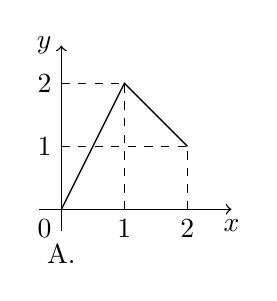
\begin{tikzpicture}[scale=0.8,line width=0.5pt]
\draw[->] (-0.35,0)--(2.7,0) node[below]{$x$};
\draw[->] (0,-0.35)--(0,2.6) node[left]{$y$};
\draw[dashed] (0,1)--(2,1) (0,2)--(1,2) (1,0)--(1,2) (2,0)--(2,1);
\draw (0,0)--(1,2)--(2,1);
\node[below left] at (0,0) {$0$};
\node[below] at (1,0) {$1$}; \node[below] at (2,0) {$2$};
\node[left] at (0,1) {$1$}; \node[left] at (0,2) {$2$};
\node[anchor=north] at (0,-0.4) {A.};
\end{tikzpicture}
&
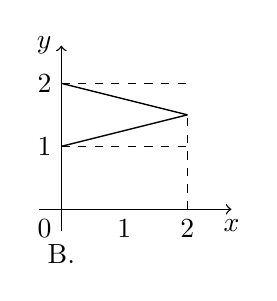
\begin{tikzpicture}[scale=0.8,line width=0.5pt]
\draw[->] (-0.35,0)--(2.7,0) node[below]{$x$};
\draw[->] (0,-0.35)--(0,2.6) node[left]{$y$};
\draw[dashed] (0,1)--(2,1) (0,2)--(2,2) (2,0)--(2,1.5);
\draw (0,2)--(2,1.5);
\draw (0,1)--(2,1.5);
\node[below left] at (0,0) {$0$};
\node[below] at (1,0) {$1$}; \node[below] at (2,0) {$2$};
\node[left] at (0,1) {$1$}; \node[left] at (0,2) {$2$};
\node[anchor=north] at (0,-0.4) {B.};
\end{tikzpicture}
\\[12pt]
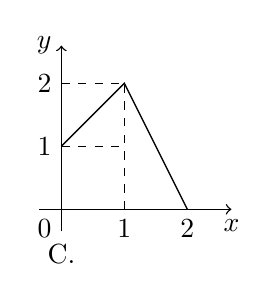
\begin{tikzpicture}[scale=0.8,line width=0.5pt]
\draw[->] (-0.35,0)--(2.7,0) node[below]{$x$};
\draw[->] (0,-0.35)--(0,2.6) node[left]{$y$};
\draw[dashed] (0,1)--(1,1) (0,2)--(1,2) (1,0)--(1,2);
\draw (0,1)--(1,2)--(2,0);
\node[below left] at (0,0) {$0$};
\node[below] at (1,0) {$1$}; \node[below] at (2,0) {$2$};
\node[left] at (0,1) {$1$}; \node[left] at (0,2) {$2$};
\node[anchor=north] at (0,-0.4) {C.};
\end{tikzpicture}
&
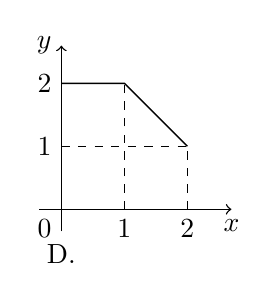
\begin{tikzpicture}[scale=0.8,line width=0.5pt]
\draw[->] (-0.35,0)--(2.7,0) node[below]{$x$};
\draw[->] (0,-0.35)--(0,2.6) node[left]{$y$};
\draw[dashed] (0,1)--(2,1) (1,0)--(1,2) (2,0)--(2,1);
\draw (0,2)--(1,2)--(2,1);
\node[below left] at (0,0) {$0$};
\node[below] at (1,0) {$1$}; \node[below] at (2,0) {$2$};
\node[left] at (0,1) {$1$}; \node[left] at (0,2) {$2$};
\node[anchor=north] at (0,-0.4) {D.};
\end{tikzpicture}
\end{tabular}
\end{center}

\ifanswer
\solbegin
\step{对于 $A$，当 $0\leqslant x\leqslant2$ 时，$0\leqslant y\leqslant2$，故 $A$ 错误；}
\step{对于 $B$，当 $0\leqslant x\leqslant2$ 时，任取一个 $x$ 的值，有两个 $y$ 与之对应，故 $B$ 错误；}
\step{对于 $C$，当 $0\leqslant x\leqslant2$ 时，$0\leqslant y\leqslant2$，故 $C$ 错误；}
\step{对于 $D$，当 $0\leqslant x\leqslant2$ 时，$0\leqslant y\leqslant2$，故 $D$ 正确.}
\step{故选 $D$.}
\solend
\fi

\item 下列函数中与函数 $y=x$ 是同一函数的是\mbox{（\quad）}

\keepwithprev
A. $y=\sqrt{x^2}$\qquad\quad B. $y=(\sqrt x)^2$\qquad\quad C. $u=\dfrac{v^2}{v}$\qquad\quad D. $m=\sqrt[5]{n^5}$

\ifanswer
\solbegin
\step{对于 $A$，$y=\sqrt{x^2}=\lvert x\rvert$，与函数 $y=x$ 的对应关系不相同，不是同一函数；}
\step{对于 $B$，$y=(\sqrt x)^2=x(x\geqslant0)$，与函数 $y=x(x\in\R)$ 的定义域不相同，不是同一函数；}
\step{对于 $C$，$u=\dfrac{v^2}{v}=v(v\neq0)$，与函数 $y=x(x\in\R)$ 的定义域不相同，不是同一函数；}
\step{对于 $D$，$m=\sqrt[5]{n^5}=n(n\in\R)$，与函数 $y=x(x\in\R)$ 的定义域相同，对应关系也相同，是同一函数.}
\step{故选 $D$.}
\solend
\fi

\item 某校高一四班学生 $46$ 人，寒假参加体育训练，其中足球队 $25$ 人，排球队 $22$ 人，游泳队 $24$ 人，足球排球都参加的有 $12$ 人，足球游泳都参加的有 $9$ 人，排球游泳都参加的有 $8$ 人，问：三项都参加的学生数为\mbox{（\quad）}

\keepwithprev
A. $2$\qquad\qquad B. $3$\qquad\qquad C. $4$\qquad\qquad D. $5$

\ifanswer
\solbegin
\step{设集合 $A=\{$参加足球队的学生$\}$，集合 $B=\{$参加排球队的学生$\}$，}
\step{集合 $C=\{$参加游泳队的学生$\}$，}
\step{则 $\operatorname{card}(A)=25$，$\operatorname{card}(B)=22$，$\operatorname{card}(C)=24$，}
\step{$\operatorname{card}(A\cap B)=12$，$\operatorname{card}(A\cap C)=9$，$\operatorname{card}(B\cap C)=8$，}
\step{设三项都参加的有 $x$ 人，即 $\operatorname{card}(A\cap B\cap C)=x$，$\operatorname{card}(A\cup B\cup C)=46$，}
\step{由 $\operatorname{card}(A\cup B\cup C)=\operatorname{card}A+\operatorname{card}B+\operatorname{card}C-\operatorname{card}(A\cap B)$}
\step{$-\operatorname{card}(B\cap C)-\operatorname{card}(A\cap C)+\operatorname{card}(A\cap B\cap C)$，}
\step{即 $46=25+22+24-12-8-9+x$，解得 $x=4$，所以三项都参加的有 $4$ 人.}
\step{故选 $C$.}
\solend
\fi

\item 已知 $\lg a$、$\lg b$ 是方程 $6x^2-4x-3=0$ 的两根，则 $\left(\lg\dfrac ab\right)^2$ 等于\mbox{（\quad）}

\keepwithprev
A. $\dfrac49$\qquad\qquad B. $\dfrac{13}{9}$\qquad\qquad C. $\dfrac{14}{9}$\qquad\qquad D. $\dfrac{22}{9}$

\ifanswer
\solbegin
\step{由韦达定理得 $\lg a+\lg b=\dfrac23$，$\lg a\cdot\lg b=-\dfrac12$，}
\step{所以 $\left(\lg\dfrac ab\right)^2=(\lg a-\lg b)^2=(\lg a+\lg b)^2-4\lg a\lg b=\dfrac49+2=\dfrac{22}{9}$. 故选 $D$.}
\solend
\fi

\end{enumerate}

\bigsec{三、解答题}

\begin{enumerate}
\setcounter{enumi}{16}

\item （1）用分数指数幂表示 $\sqrt[3]{a^2}\cdot\sqrt{a^3}$；

（2）已知 $a^{\frac12}+a^{-\frac12}=3$，求 $a+a^{-1}$.

\ifanswer
\solbegin
\step{（1）$\sqrt[3]{a^2}\cdot\sqrt{a^3}=a^{\frac23}\times a^{\frac32}=a^{\frac{13}6}$.}
\step{（2）由 $a^{\frac12}+a^{-\frac12}=3$，平方得 $a+2+a^{-1}=9$，故 $a+a^{-1}=7$.}
\solend
\fi

\item 已知 $f(x)=\begin{cases}x,x>0\\-x^2-2x+1,x\leqslant0\end{cases}$.

（1）求 $f(f(-2))$ 的值；

（2）若 $f(x_0)=2$，求 $x_0$ 的值.

\ifanswer
\solbegin
\step{（1）$f(x)=\begin{cases}x,x>0\\-x^2-2x+1,x\leqslant0\end{cases}$，则 $f(-2)=-(-2)^2-2\times(-2)+1=1$，}
\step{则有 $f(f(-2))=f(1)=1$；}
\step{（2）当 $x_0>0$ 时，$f(x_0)=x_0$，又 $f(x_0)=2$，所以 $x_0=2$，}
\step{当 $x_0\leqslant0$ 时，$f(x_0)=-x_0^2-2x_0+1$，又 $f(x_0)=2$，}
\step{所以 $-x_0^2-2x_0+1=2$，故 $x_0=-1$，}
\step{综上，$x_0$ 的值为 $-1$ 或 $2$.}
\solend
\fi

\item 已知集合 $A=\{x\mid\lvert 1+x\rvert+\lvert x\rvert<5\}$，$B=\left\{x\,\middle\vert\,\dfrac2{x-m}\geqslant1\right\}$，$p:x\in A$，$q:x\in B$.

（1）若 $m=0$，且 $p$ 真 $q$ 假，求实数 $x$ 的取值范围；

（2）若 $q$ 是 $p$ 的充分不必要条件，求实数 $m$ 的取值范围.

\ifanswer
\solbegin
\step{（1）当 $x\geqslant0$ 时，不等式 $\lvert 1+x\rvert+\lvert x\rvert<5$ 化为 $1+x+x<5$，解得 $0\leqslant x<2$；}
\step{当 $-1\leqslant x<0$ 时，不等式 $\lvert 1+x\rvert+\lvert x\rvert<5$ 化为 $1+x-x<5$ 恒成立，}
\step{故 $-1\leqslant x<0$；}
\step{当 $x<-1$ 时，不等式 $\lvert 1+x\rvert+\lvert x\rvert<5$ 化为 $-1-x-x<5$，}
\step{解得 $-3<x<-1$.}
\step{综上所述，$\lvert 1+x\rvert+\lvert x\rvert<5$ 等价于 $-3<x<2$，}
\step{所以 $\lvert 1+x\rvert+\lvert x\rvert<5$ 的解集为 $A=(-3,2)$，}
\step{若 $m=0$，则 $B=\left\{x\,\middle\vert\,\dfrac2x\geqslant1\right\}=\{x\mid 0<x\leqslant2\}$，得 $\overline{B}=(-\infty,0]\cup(2,+\infty)$，}
\step{由 $p$ 真 $q$ 假，得 $x\in(A\cap\overline{B})=(-3,0]$，即 $x$ 的取值范围为 $(-3,0]$；}
\step{（2）由 $\dfrac2{x-m}\geqslant1$，得 $\begin{cases}x-m>0\\x-m\leqslant2\end{cases}$，解得 $m<x\leqslant m+2$，}
\step{所以 $B=\left\{x\,\middle\vert\,\dfrac2{x-m}\geqslant1\right\}=(m,m+2]$，}
\step{由（1）的结论，得 $A=(-3,2)$，}
\step{若 $q$ 是 $p$ 的充分不必要条件，则 $B$ 是 $A$ 的真子集，得 $\begin{cases}m\geqslant-3\\m+2<2\end{cases}$，}
\step{解得 $-3\leqslant m<0$，即实数 $m$ 的取值范围是 $[-3,0)$.}
\solend
\fi

\item 某企业计划在 $2026$ 年布局人工智能大模型应用开发，生产智能终端配套的 $AI$ 算法服务包. 通过市场分析，全年需投入固定成本 $260$ 万元（含研发、服务器部署等），每生产 $x$ 千个算法服务包，需另投入成本 $R(x)$ 万元，且
$R(x)=\begin{cases}10x^2+100x,0<x\leqslant40\\601x+\dfrac{10000}{x}-7260,x>40\end{cases}$. 已知每个算法服务包的售价为 $0.6$ 万元，假设年内生产的服务包当年能全部销售完.

（1）试写出 $2026$ 年利润 $L$（万元）关于年产量 $x$（千个）的函数解析式；

（2）当 $2026$ 年产量为多少千个时，企业所获利润最大？并求出最大利润.

\ifanswer
\solbegin
\step{（1）$L(x)=x\cdot1000\times0.6-R(x)-260=600x-R(x)-260$，}
\step{当 $0<x\leqslant40$ 时，}
\step{$L(x)=600x-(10x^2+100x)-260=-10x^2+500x-260$；}
\step{当 $x>40$ 时，}
\step{$L(x)=600x-\left(601x+\dfrac{10000}{x}-7260\right)-260=7000-x-\dfrac{10000}{x}$；}
\step{综上，$L(x)=\begin{cases}-10x^2+500x-260,0<x\leqslant40\\7000-x-\dfrac{10000}{x},x>40\end{cases}$；}
\step{（2）当 $0<x\leqslant40$ 时，$L(x)=-10x^2+500x-260=-10(x-25)^2+5990$，}
\step{当 $x=25$ 时，函数 $L(x)$ 有最大值 $5990$；}
\step{当 $x>40$ 时，$L(x)=7000-x-\dfrac{10000}{x}=7000-\left(x+\dfrac{10000}{x}\right)$}
\step{$\leqslant7000-2\sqrt{x\cdot\dfrac{10000}{x}}=7000-2\times100=6800$，}
\step{当且仅当 $x=\dfrac{10000}{x}$ 时取等号，}
\step{所以当 $x=100$ 时，函数 $L(x)$ 有最大值 $6800$；}
\step{因为 $6800>5990$，所以 $2026$ 年产量为 $100$ 千个时，企业所获利润最大，}
\step{最大利润为 $6800$ 万元.}
\solend
\fi

\item 已知二次函数 $f(x)=ax^2+bx+c$.

（1）若 $f(x)>0$ 的解集为 $\{x\mid-3<x<4\}$，解关于 $x$ 的不等式 $bx^2+2ax-(c+3b)<0$；

（2）若函数满足 $f(x+1)-f(x)=2x+2$，且 $f(0)=1$. 求 $f(x)$ 的解析式；

（3）若对任意 $x\in\R$，不等式 $f(x)\geqslant2ax+b$ 恒成立，求 $\dfrac{b^2}{4(a^2+c^2)}$ 的最大值.

\ifanswer
\solbegin
\step{（1）由题意二次函数 $f(x)=ax^2+bx+c$，}
\step{若 $f(x)>0$ 的解集为 $\{x\mid-3<x<4\}$，}
\step{得 $-3$、$4$ 为方程 $ax^2+bx+c=0$ 的根，且 $a<0$，}
\step{则 $\begin{cases}-3+4=-\dfrac ba\\-3\times4=\dfrac ca\end{cases}$，即 $b=-a$，$c=-12a$，}
\step{则不等式 $bx^2+2ax-(c+3b)<0$，即为 $-ax^2+2ax+15a<0(a<0)$，}
\step{则 $x^2-2x-15<0$，解得 $-3<x<5$，}
\step{所以不等式 $bx^2+2ax-(c+3b)<0$ 的解集为 $(-3,5)$；}
\step{（2）由 $f(x)=ax^2+bx+c(a\neq0)$，}
\step{则 $f(x+1)-f(x)=a(x+1)^2+b(x+1)+c-(ax^2+bx+c)=2ax+a+b$，}
\step{又 $f(x+1)-f(x)=2x+2$，故 $\begin{cases}2a=2\\a+b=2\end{cases}$，解得 $a=1$，$b=1$，}
\step{由 $f(0)=1$，得 $c=1$，所以 $f(x)=x^2+x+1$；}
\step{（3）由题意二次函数 $f(x)=ax^2+bx+c$，}
\step{若对任意 $x\in\R$，不等式 $f(x)\geqslant2ax+b$ 恒成立，}
\step{得对任意 $x\in\R$，$ax^2+bx+c\geqslant2ax+b$ 恒成立，}
\step{整理得 $ax^2+(b-2a)x+c-b\geqslant0$ 恒成立，}
\step{因为 $a$ 不为 $0$，所以 $\begin{cases}a>0\\\Delta=(b-2a)^2-4a(c-b)\leqslant0\end{cases}$，}
\step{所以 $0\leqslant b^2\leqslant4a(c-a)$，所以 $\dfrac{b^2}{4(a^2+c^2)}\leqslant\dfrac{ac-a^2}{a^2+c^2}=\dfrac{\frac ca-1}{1+\left(\frac ca\right)^2}$，}
\step{令 $t=\dfrac ca-1$，因为 $0\leqslant b^2\leqslant4a(c-a)$，所以 $c\geqslant a>0\Rightarrow t\geqslant0$，}
\step{若 $t=0$ 时，此时 $\dfrac{b^2}{4(a^2+c^2)}\leqslant\dfrac{\frac ca-1}{1+\left(\frac ca\right)^2}=0$，}
\step{若 $t>0$ 时，$\dfrac{b^2}{4(a^2+c^2)}\leqslant\dfrac{t}{1+(t+1)^2}=\dfrac{t}{t^2+2t+2}=\dfrac1{t+\frac2t+2}$}
\step{$\leqslant\dfrac1{2\sqrt2+2}=\dfrac{\sqrt2-1}{2}$，}
\step{当且仅当 $t=\dfrac2t$，即 $t=\sqrt2$ 时，即 $c=(1+\sqrt2)a$ 时，上式取等号.}
\step{综上所述，$\dfrac{b^2}{4(a^2+c^2)}$ 的最大值为 $\dfrac{\sqrt2-1}{2}$.}
\solend
\fi

\end{enumerate}

\end{document}
"
% 紧凑版：xelatex "\def\iscompact{1}% 高一117_陆行中学_期中.tex
%   —— 高一上数学“2026-2027 年陆行中学高一上期中”（试卷版/答案版）
% 试卷版：xelatex 高一117_陆行中学_期中.tex
% 答案版：xelatex "\def\isanswer{1}% 高一117_陆行中学_期中.tex
%   —— 高一上数学“2026-2027 年陆行中学高一上期中”（试卷版/答案版）
% 试卷版：xelatex 高一117_陆行中学_期中.tex
% 答案版：xelatex "\def\isanswer{1}\input{高一117_陆行中学_期中.tex}"
% 紧凑版：xelatex "\def\iscompact{1}\input{高一117_陆行中学_期中.tex}"
%
% 原始材料：微信公众号“魔都数学加油站”文章，作者破晓，2026-11-06 17:58 发布；
% 连载“27学年高一117”，原文标题“27学年高一117——2026-2027年上海市陆行中学高一上期中”；
% 原文链接：https://mp.weixin.qq.com/s/of8iPW26dvDyXWohudT0vw。
% 正文为 10 张 PNG 页（第 1、3、4、8、9、10 页 2560×3620，其余 4762×6735），
% 题目下印有【解析】或【答案】，为讲评版。
% 题目、解析均据原图转录；卷面红色水印及公众号页脚未录入。
%
% 卷首标题：原卷印作“2026-2027 年陆行中学高一上期中”（公众号标题中的“上海市”
% 卷面标题行没有，本稿照卷面），年份区间按全稿惯例排 en dash；原卷未印副标题，本稿按题目内容
% 标为“集合与常用逻辑用语、不等式、函数”（期中卷跨三章，含指数／对数与函数，与 112 同）。
%
% 与原卷的排版差异：
%   ① 原文从第 3 题起，填空题 3—12、选择题 13—16、解答题 17—21，共 19 题，本稿保留原题号；
%   ② 原卷每题下直接印【解析】／【答案】，本稿按全稿惯例置于答案版；第 4、6、8 题只印
%      【答案】，另提 \ans{}；其余选择题答案在解析末句“故选 …”，括号内留空；
%   ③ 原卷未印副标题，本稿按“知识模块”口径补出；
%   ④ 原卷填空横线按全稿惯例排为 \blankline[4.4em]；选择题括号排 \mbox{（\quad）}、
%      选项段前按惯例加 \keepwithprev；解答题不留作答区（原卷为讲评版，与 109—116 同）；
%   ⑤ 原卷 $max$／$min$ 排斜体，按 96 成例改 \max／\min；数集 $R$ 按惯例改 \R。
%
% 判别式字形：第 11 题与第 21 题 (3) 的判别式原卷排 $\Delta$（等腰、右厚），照录 \Delta。
%
% 子集符号：第 5 题的 $B\subseteq A$ 印有下划线，照录 \subseteq。
%
% 第 13 题四个坐标图选项按原图形状用 TikZ 重排（三版都出）；原卷另有第 12 题的
%   $a\odot b$ 自定义运算、第 15 题的 $\operatorname{card}$ 记号，均照录。
%
% 原卷存疑照录：第 12 题解析的 $\min\{\left|x\right|\odot\left|3-x\right|\}$ 一行、
%   第 20 题 $R(x)$ 分段函数与 $L(x)$ 的推导，均按原卷印刷行照录。
%   第 20 题题干开头原卷有一段会议背景引语（非数学信息），本稿从“某企业计划在
%   $2026$ 年布局…”起照录题目主体，全部数据、设问与解析均完整保留。
%
% 行数核对：逐题数 \step/\stepm 条数，合计 106 条（Q3：1；Q4：0；Q5：5；Q6：0；Q7：3；
% Q8：0；Q9：3；Q10：3；Q11：5；Q12：6；Q13：5；Q14：5；Q15：9；Q16：2；Q17：2；
% Q18：6；Q19：14；Q20：14；Q21：23），与原卷印刷行逐题相等（cases／TikZ 图块作一个
% 印刷行计）。第 4、6、8 题只印【答案】，提 \ans{}，不计入 \step 账。
%
\documentclass[a4paper,11pt]{article}
\usepackage{common}

\begin{document}

\examtitlest[3]{2026--2027 年陆行中学高一上期中}{集合与常用逻辑用语、不等式、函数}

\bigsec{一、填空题}

\begin{enumerate}
\setcounter{enumi}{2}

\item 已知 $10^a=2$,$10^b=5$，则 $10^{3a-2b}$ 的值为\blankline[4.4em].

\ifanswer
\solbegin
\step{$10^{3a-2b}=\dfrac{10^{3a}}{10^{2b}}=\dfrac{(10^a)^3}{(10^b)^2}=\dfrac{2^3}{5^2}=\dfrac8{25}$.}
\solend
\fi

\item 已知不等式 $\lvert x+1\rvert+\lvert x-3\rvert\geqslant4$ 恒成立，则取等号时 $x$ 的取值范围是\blankline[4.4em].

\ifanswer
\ans{$[-1,3]$}
\fi

\item 集合 $A=\{1,2,a^2\}$，$B=\{2,a\}$，若 $B\subseteq A$，则 $a$ 的值为\blankline[4.4em].

\ifanswer
\solbegin
\step{因为 $B\subseteq A$，所以 $a=1$ 或 $a=a^2$，}
\step{当 $a=1$ 时，$a^2=1$，不满足元素的互异性，故舍去；}
\step{当 $a=a^2$ 时，解得 $a=1$（舍）或 $a=0$，}
\step{当 $a=0$ 时，$A=\{1,2,0\}$，$B=\{2,0\}$，满足题意.}
\step{综上，$a=0$.}
\solend
\fi

\item 若 $x>\dfrac35$，则 $y=5x+\dfrac1{5x-3}$ 的最小值是\blankline[4.4em].

\ifanswer
\ans{$5$}
\fi

\item 已知 $a>0$，$b>0$，且 $a+b=1$，则 $\dfrac3a+\dfrac1b$ 的最小值是\blankline[4.4em].

\ifanswer
\solbegin
\step{$a>0$，$b>0$，且 $a+b=1$，}
\step{$\dfrac3a+\dfrac1b=\left(\dfrac3a+\dfrac1b\right)(a+b)=\dfrac{3b}{a}+\dfrac ab+4\geqslant2\sqrt3+4$，}
\step{当且仅当 $\dfrac{3b}{a}=\dfrac ab$ 时取等号，所以 $\dfrac3a+\dfrac1b$ 的最小值为 $2\sqrt3+4$.}
\solend
\fi

\item 已知 $\log_2 5=a$，则 $\log_5 10=$\blankline[4.4em]（用含 $a$ 的代数式表示）.

\ifanswer
\ans{$1+\dfrac1a$}
\fi

\item 已知 $p:2<x\leqslant3$，$q:\lvert x-a\rvert<2$，若 $p$ 是 $q$ 的充分不必要条件，则实数 $a$ 的取值范围为\blankline[4.4em].

\ifanswer
\solbegin
\step{由 $\lvert x-a\rvert<2$ 得 $a-2<x<a+2$，即 $p:2<x\leqslant3$，$q:a-2<x<a+2$.}
\step{因为 $p$ 是 $q$ 的充分不必要条件，所以 $\begin{cases}a-2\leqslant2\\a+2>3\end{cases}$，解得 $1<a\leqslant4$，}
\step{所以实数 $a$ 的取值范围为 $(1,4]$.}
\solend
\fi

\item 已知 $a>1$,$b>1$，若 $\log_a b+\log_b a=2$，且 $ab=2$，则 $\log_2(a+b)=$\blankline[4.4em].

\ifanswer
\solbegin
\step{由 $\log_a b+\log_b a=2$,$a>1$,$b>1$，得 $\log_a b+\dfrac1{\log_a b}=2$，}
\step{即 $(\log_a b)^2-2\log_a b+1=0$，则 $(\log_a b-1)^2=0$，即 $\log_a b=1$，则 $a=b$，}
\step{又 $ab=2$，则 $a=b=\sqrt2$，所以 $\log_2(a+b)=\log_2(2\sqrt2)=\log_2 2^{\frac32}=\dfrac32$.}
\solend
\fi

\item 已知函数 $f(x)=\sqrt{2kx^2+kx+\dfrac34}$ 的定义域为实数集 $\R$，则实数 $k$ 的取值范围\blankline[4.4em].

\ifanswer
\solbegin
\step{因为函数 $f(x)=\sqrt{2kx^2+kx+\dfrac34}$ 的定义域为实数集 $\R$，}
\step{所以 $2kx^2+kx+\dfrac34\geqslant0$ 在 $\R$ 上恒成立，}
\step{当 $k=0$ 时，$\dfrac34\geqslant0$，恒成立；}
\step{当 $k\neq0$ 时，则有 $\begin{cases}2k>0\\\Delta=k^2-4\times2k\times\dfrac34\leqslant0\end{cases}$，解得 $0<k\leqslant6$；}
\step{综上，实数 $k$ 的取值范围为 $[0,6]$.}
\solend
\fi

\item 对于两个实数 $a$、$b$，定义运算 $a\odot b$ 如下：若 $a\geqslant b$，则 $a\odot b=a$；若 $a<b$，则 $a\odot b=b$. 若 $x$、$y\in\R$，则 $\lvert x-y\rvert\odot\lvert 3-x\rvert\odot\lvert x+y\rvert$ 的最小值是\blankline[4.4em].

\ifanswer
\solbegin
\step{由题意得 $a\odot b=\max\{a,b\}$，所以 $\lvert a+b\rvert\odot\lvert a-b\rvert=\max\{\lvert a+b\rvert,\lvert a-b\rvert\}$，}
\step{设 $\max\{\lvert a+b\rvert,\lvert a-b\rvert\}=M$，则 $\begin{cases}M\geqslant\lvert a+b\rvert\\M\geqslant\lvert a-b\rvert\end{cases}$，}
\step{所以 $2M\geqslant\lvert a+b\rvert+\lvert a-b\rvert\geqslant2\lvert a\rvert$，则 $\lvert a+b\rvert\odot\lvert a-b\rvert\geqslant\lvert a\rvert$，}
\step{所以 $\min\{\lvert x-y\rvert\odot\lvert 3-x\rvert\odot\lvert x+y\rvert\}=\min\{\lvert x-y\rvert\odot\lvert x+y\rvert\odot\lvert 3-x\rvert\}$}
\step{$=\min\{\lvert x\rvert\odot\lvert 3-x\rvert\}=\min\left\{\dfrac32+x\odot\left\lvert\dfrac32-x\right\rvert\right\}=\dfrac32$，}% 原卷该行写法照录
\step{当且仅当 $x=\dfrac32$，$y=0$ 取等号，故 $\lvert x-y\rvert\odot\lvert 3-x\rvert\odot\lvert x+y\rvert$ 的最小值是 $\dfrac32$.}
\solend
\fi

\end{enumerate}

\bigsec{二、选择题}

\begin{enumerate}
\setcounter{enumi}{12}

\item 设 $A=\{x\mid 0\leqslant x\leqslant2\}$，$B=\{y\mid 1\leqslant y\leqslant2\}$，下列图形能表示从集合 $A$ 到集合 $B$ 的函数图像的是\mbox{（\quad）}

\keepwithprev
\begin{center}
% 原卷四个坐标图选项按原图形状用 TikZ 重排。
\begin{tabular}{c@{\qquad\qquad}c}
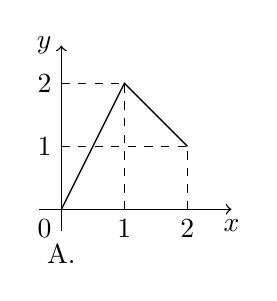
\begin{tikzpicture}[scale=0.8,line width=0.5pt]
\draw[->] (-0.35,0)--(2.7,0) node[below]{$x$};
\draw[->] (0,-0.35)--(0,2.6) node[left]{$y$};
\draw[dashed] (0,1)--(2,1) (0,2)--(1,2) (1,0)--(1,2) (2,0)--(2,1);
\draw (0,0)--(1,2)--(2,1);
\node[below left] at (0,0) {$0$};
\node[below] at (1,0) {$1$}; \node[below] at (2,0) {$2$};
\node[left] at (0,1) {$1$}; \node[left] at (0,2) {$2$};
\node[anchor=north] at (0,-0.4) {A.};
\end{tikzpicture}
&
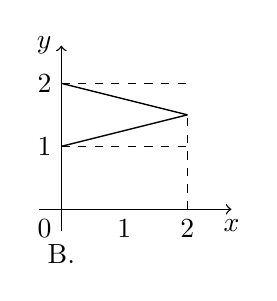
\begin{tikzpicture}[scale=0.8,line width=0.5pt]
\draw[->] (-0.35,0)--(2.7,0) node[below]{$x$};
\draw[->] (0,-0.35)--(0,2.6) node[left]{$y$};
\draw[dashed] (0,1)--(2,1) (0,2)--(2,2) (2,0)--(2,1.5);
\draw (0,2)--(2,1.5);
\draw (0,1)--(2,1.5);
\node[below left] at (0,0) {$0$};
\node[below] at (1,0) {$1$}; \node[below] at (2,0) {$2$};
\node[left] at (0,1) {$1$}; \node[left] at (0,2) {$2$};
\node[anchor=north] at (0,-0.4) {B.};
\end{tikzpicture}
\\[12pt]
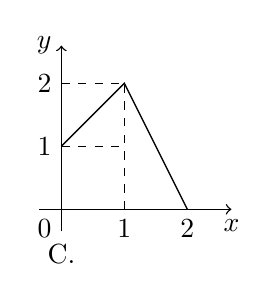
\begin{tikzpicture}[scale=0.8,line width=0.5pt]
\draw[->] (-0.35,0)--(2.7,0) node[below]{$x$};
\draw[->] (0,-0.35)--(0,2.6) node[left]{$y$};
\draw[dashed] (0,1)--(1,1) (0,2)--(1,2) (1,0)--(1,2);
\draw (0,1)--(1,2)--(2,0);
\node[below left] at (0,0) {$0$};
\node[below] at (1,0) {$1$}; \node[below] at (2,0) {$2$};
\node[left] at (0,1) {$1$}; \node[left] at (0,2) {$2$};
\node[anchor=north] at (0,-0.4) {C.};
\end{tikzpicture}
&
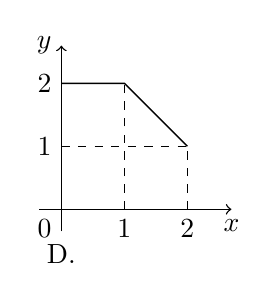
\begin{tikzpicture}[scale=0.8,line width=0.5pt]
\draw[->] (-0.35,0)--(2.7,0) node[below]{$x$};
\draw[->] (0,-0.35)--(0,2.6) node[left]{$y$};
\draw[dashed] (0,1)--(2,1) (1,0)--(1,2) (2,0)--(2,1);
\draw (0,2)--(1,2)--(2,1);
\node[below left] at (0,0) {$0$};
\node[below] at (1,0) {$1$}; \node[below] at (2,0) {$2$};
\node[left] at (0,1) {$1$}; \node[left] at (0,2) {$2$};
\node[anchor=north] at (0,-0.4) {D.};
\end{tikzpicture}
\end{tabular}
\end{center}

\ifanswer
\solbegin
\step{对于 $A$，当 $0\leqslant x\leqslant2$ 时，$0\leqslant y\leqslant2$，故 $A$ 错误；}
\step{对于 $B$，当 $0\leqslant x\leqslant2$ 时，任取一个 $x$ 的值，有两个 $y$ 与之对应，故 $B$ 错误；}
\step{对于 $C$，当 $0\leqslant x\leqslant2$ 时，$0\leqslant y\leqslant2$，故 $C$ 错误；}
\step{对于 $D$，当 $0\leqslant x\leqslant2$ 时，$0\leqslant y\leqslant2$，故 $D$ 正确.}
\step{故选 $D$.}
\solend
\fi

\item 下列函数中与函数 $y=x$ 是同一函数的是\mbox{（\quad）}

\keepwithprev
A. $y=\sqrt{x^2}$\qquad\quad B. $y=(\sqrt x)^2$\qquad\quad C. $u=\dfrac{v^2}{v}$\qquad\quad D. $m=\sqrt[5]{n^5}$

\ifanswer
\solbegin
\step{对于 $A$，$y=\sqrt{x^2}=\lvert x\rvert$，与函数 $y=x$ 的对应关系不相同，不是同一函数；}
\step{对于 $B$，$y=(\sqrt x)^2=x(x\geqslant0)$，与函数 $y=x(x\in\R)$ 的定义域不相同，不是同一函数；}
\step{对于 $C$，$u=\dfrac{v^2}{v}=v(v\neq0)$，与函数 $y=x(x\in\R)$ 的定义域不相同，不是同一函数；}
\step{对于 $D$，$m=\sqrt[5]{n^5}=n(n\in\R)$，与函数 $y=x(x\in\R)$ 的定义域相同，对应关系也相同，是同一函数.}
\step{故选 $D$.}
\solend
\fi

\item 某校高一四班学生 $46$ 人，寒假参加体育训练，其中足球队 $25$ 人，排球队 $22$ 人，游泳队 $24$ 人，足球排球都参加的有 $12$ 人，足球游泳都参加的有 $9$ 人，排球游泳都参加的有 $8$ 人，问：三项都参加的学生数为\mbox{（\quad）}

\keepwithprev
A. $2$\qquad\qquad B. $3$\qquad\qquad C. $4$\qquad\qquad D. $5$

\ifanswer
\solbegin
\step{设集合 $A=\{$参加足球队的学生$\}$，集合 $B=\{$参加排球队的学生$\}$，}
\step{集合 $C=\{$参加游泳队的学生$\}$，}
\step{则 $\operatorname{card}(A)=25$，$\operatorname{card}(B)=22$，$\operatorname{card}(C)=24$，}
\step{$\operatorname{card}(A\cap B)=12$，$\operatorname{card}(A\cap C)=9$，$\operatorname{card}(B\cap C)=8$，}
\step{设三项都参加的有 $x$ 人，即 $\operatorname{card}(A\cap B\cap C)=x$，$\operatorname{card}(A\cup B\cup C)=46$，}
\step{由 $\operatorname{card}(A\cup B\cup C)=\operatorname{card}A+\operatorname{card}B+\operatorname{card}C-\operatorname{card}(A\cap B)$}
\step{$-\operatorname{card}(B\cap C)-\operatorname{card}(A\cap C)+\operatorname{card}(A\cap B\cap C)$，}
\step{即 $46=25+22+24-12-8-9+x$，解得 $x=4$，所以三项都参加的有 $4$ 人.}
\step{故选 $C$.}
\solend
\fi

\item 已知 $\lg a$、$\lg b$ 是方程 $6x^2-4x-3=0$ 的两根，则 $\left(\lg\dfrac ab\right)^2$ 等于\mbox{（\quad）}

\keepwithprev
A. $\dfrac49$\qquad\qquad B. $\dfrac{13}{9}$\qquad\qquad C. $\dfrac{14}{9}$\qquad\qquad D. $\dfrac{22}{9}$

\ifanswer
\solbegin
\step{由韦达定理得 $\lg a+\lg b=\dfrac23$，$\lg a\cdot\lg b=-\dfrac12$，}
\step{所以 $\left(\lg\dfrac ab\right)^2=(\lg a-\lg b)^2=(\lg a+\lg b)^2-4\lg a\lg b=\dfrac49+2=\dfrac{22}{9}$. 故选 $D$.}
\solend
\fi

\end{enumerate}

\bigsec{三、解答题}

\begin{enumerate}
\setcounter{enumi}{16}

\item （1）用分数指数幂表示 $\sqrt[3]{a^2}\cdot\sqrt{a^3}$；

（2）已知 $a^{\frac12}+a^{-\frac12}=3$，求 $a+a^{-1}$.

\ifanswer
\solbegin
\step{（1）$\sqrt[3]{a^2}\cdot\sqrt{a^3}=a^{\frac23}\times a^{\frac32}=a^{\frac{13}6}$.}
\step{（2）由 $a^{\frac12}+a^{-\frac12}=3$，平方得 $a+2+a^{-1}=9$，故 $a+a^{-1}=7$.}
\solend
\fi

\item 已知 $f(x)=\begin{cases}x,x>0\\-x^2-2x+1,x\leqslant0\end{cases}$.

（1）求 $f(f(-2))$ 的值；

（2）若 $f(x_0)=2$，求 $x_0$ 的值.

\ifanswer
\solbegin
\step{（1）$f(x)=\begin{cases}x,x>0\\-x^2-2x+1,x\leqslant0\end{cases}$，则 $f(-2)=-(-2)^2-2\times(-2)+1=1$，}
\step{则有 $f(f(-2))=f(1)=1$；}
\step{（2）当 $x_0>0$ 时，$f(x_0)=x_0$，又 $f(x_0)=2$，所以 $x_0=2$，}
\step{当 $x_0\leqslant0$ 时，$f(x_0)=-x_0^2-2x_0+1$，又 $f(x_0)=2$，}
\step{所以 $-x_0^2-2x_0+1=2$，故 $x_0=-1$，}
\step{综上，$x_0$ 的值为 $-1$ 或 $2$.}
\solend
\fi

\item 已知集合 $A=\{x\mid\lvert 1+x\rvert+\lvert x\rvert<5\}$，$B=\left\{x\,\middle\vert\,\dfrac2{x-m}\geqslant1\right\}$，$p:x\in A$，$q:x\in B$.

（1）若 $m=0$，且 $p$ 真 $q$ 假，求实数 $x$ 的取值范围；

（2）若 $q$ 是 $p$ 的充分不必要条件，求实数 $m$ 的取值范围.

\ifanswer
\solbegin
\step{（1）当 $x\geqslant0$ 时，不等式 $\lvert 1+x\rvert+\lvert x\rvert<5$ 化为 $1+x+x<5$，解得 $0\leqslant x<2$；}
\step{当 $-1\leqslant x<0$ 时，不等式 $\lvert 1+x\rvert+\lvert x\rvert<5$ 化为 $1+x-x<5$ 恒成立，}
\step{故 $-1\leqslant x<0$；}
\step{当 $x<-1$ 时，不等式 $\lvert 1+x\rvert+\lvert x\rvert<5$ 化为 $-1-x-x<5$，}
\step{解得 $-3<x<-1$.}
\step{综上所述，$\lvert 1+x\rvert+\lvert x\rvert<5$ 等价于 $-3<x<2$，}
\step{所以 $\lvert 1+x\rvert+\lvert x\rvert<5$ 的解集为 $A=(-3,2)$，}
\step{若 $m=0$，则 $B=\left\{x\,\middle\vert\,\dfrac2x\geqslant1\right\}=\{x\mid 0<x\leqslant2\}$，得 $\overline{B}=(-\infty,0]\cup(2,+\infty)$，}
\step{由 $p$ 真 $q$ 假，得 $x\in(A\cap\overline{B})=(-3,0]$，即 $x$ 的取值范围为 $(-3,0]$；}
\step{（2）由 $\dfrac2{x-m}\geqslant1$，得 $\begin{cases}x-m>0\\x-m\leqslant2\end{cases}$，解得 $m<x\leqslant m+2$，}
\step{所以 $B=\left\{x\,\middle\vert\,\dfrac2{x-m}\geqslant1\right\}=(m,m+2]$，}
\step{由（1）的结论，得 $A=(-3,2)$，}
\step{若 $q$ 是 $p$ 的充分不必要条件，则 $B$ 是 $A$ 的真子集，得 $\begin{cases}m\geqslant-3\\m+2<2\end{cases}$，}
\step{解得 $-3\leqslant m<0$，即实数 $m$ 的取值范围是 $[-3,0)$.}
\solend
\fi

\item 某企业计划在 $2026$ 年布局人工智能大模型应用开发，生产智能终端配套的 $AI$ 算法服务包. 通过市场分析，全年需投入固定成本 $260$ 万元（含研发、服务器部署等），每生产 $x$ 千个算法服务包，需另投入成本 $R(x)$ 万元，且
$R(x)=\begin{cases}10x^2+100x,0<x\leqslant40\\601x+\dfrac{10000}{x}-7260,x>40\end{cases}$. 已知每个算法服务包的售价为 $0.6$ 万元，假设年内生产的服务包当年能全部销售完.

（1）试写出 $2026$ 年利润 $L$（万元）关于年产量 $x$（千个）的函数解析式；

（2）当 $2026$ 年产量为多少千个时，企业所获利润最大？并求出最大利润.

\ifanswer
\solbegin
\step{（1）$L(x)=x\cdot1000\times0.6-R(x)-260=600x-R(x)-260$，}
\step{当 $0<x\leqslant40$ 时，}
\step{$L(x)=600x-(10x^2+100x)-260=-10x^2+500x-260$；}
\step{当 $x>40$ 时，}
\step{$L(x)=600x-\left(601x+\dfrac{10000}{x}-7260\right)-260=7000-x-\dfrac{10000}{x}$；}
\step{综上，$L(x)=\begin{cases}-10x^2+500x-260,0<x\leqslant40\\7000-x-\dfrac{10000}{x},x>40\end{cases}$；}
\step{（2）当 $0<x\leqslant40$ 时，$L(x)=-10x^2+500x-260=-10(x-25)^2+5990$，}
\step{当 $x=25$ 时，函数 $L(x)$ 有最大值 $5990$；}
\step{当 $x>40$ 时，$L(x)=7000-x-\dfrac{10000}{x}=7000-\left(x+\dfrac{10000}{x}\right)$}
\step{$\leqslant7000-2\sqrt{x\cdot\dfrac{10000}{x}}=7000-2\times100=6800$，}
\step{当且仅当 $x=\dfrac{10000}{x}$ 时取等号，}
\step{所以当 $x=100$ 时，函数 $L(x)$ 有最大值 $6800$；}
\step{因为 $6800>5990$，所以 $2026$ 年产量为 $100$ 千个时，企业所获利润最大，}
\step{最大利润为 $6800$ 万元.}
\solend
\fi

\item 已知二次函数 $f(x)=ax^2+bx+c$.

（1）若 $f(x)>0$ 的解集为 $\{x\mid-3<x<4\}$，解关于 $x$ 的不等式 $bx^2+2ax-(c+3b)<0$；

（2）若函数满足 $f(x+1)-f(x)=2x+2$，且 $f(0)=1$. 求 $f(x)$ 的解析式；

（3）若对任意 $x\in\R$，不等式 $f(x)\geqslant2ax+b$ 恒成立，求 $\dfrac{b^2}{4(a^2+c^2)}$ 的最大值.

\ifanswer
\solbegin
\step{（1）由题意二次函数 $f(x)=ax^2+bx+c$，}
\step{若 $f(x)>0$ 的解集为 $\{x\mid-3<x<4\}$，}
\step{得 $-3$、$4$ 为方程 $ax^2+bx+c=0$ 的根，且 $a<0$，}
\step{则 $\begin{cases}-3+4=-\dfrac ba\\-3\times4=\dfrac ca\end{cases}$，即 $b=-a$，$c=-12a$，}
\step{则不等式 $bx^2+2ax-(c+3b)<0$，即为 $-ax^2+2ax+15a<0(a<0)$，}
\step{则 $x^2-2x-15<0$，解得 $-3<x<5$，}
\step{所以不等式 $bx^2+2ax-(c+3b)<0$ 的解集为 $(-3,5)$；}
\step{（2）由 $f(x)=ax^2+bx+c(a\neq0)$，}
\step{则 $f(x+1)-f(x)=a(x+1)^2+b(x+1)+c-(ax^2+bx+c)=2ax+a+b$，}
\step{又 $f(x+1)-f(x)=2x+2$，故 $\begin{cases}2a=2\\a+b=2\end{cases}$，解得 $a=1$，$b=1$，}
\step{由 $f(0)=1$，得 $c=1$，所以 $f(x)=x^2+x+1$；}
\step{（3）由题意二次函数 $f(x)=ax^2+bx+c$，}
\step{若对任意 $x\in\R$，不等式 $f(x)\geqslant2ax+b$ 恒成立，}
\step{得对任意 $x\in\R$，$ax^2+bx+c\geqslant2ax+b$ 恒成立，}
\step{整理得 $ax^2+(b-2a)x+c-b\geqslant0$ 恒成立，}
\step{因为 $a$ 不为 $0$，所以 $\begin{cases}a>0\\\Delta=(b-2a)^2-4a(c-b)\leqslant0\end{cases}$，}
\step{所以 $0\leqslant b^2\leqslant4a(c-a)$，所以 $\dfrac{b^2}{4(a^2+c^2)}\leqslant\dfrac{ac-a^2}{a^2+c^2}=\dfrac{\frac ca-1}{1+\left(\frac ca\right)^2}$，}
\step{令 $t=\dfrac ca-1$，因为 $0\leqslant b^2\leqslant4a(c-a)$，所以 $c\geqslant a>0\Rightarrow t\geqslant0$，}
\step{若 $t=0$ 时，此时 $\dfrac{b^2}{4(a^2+c^2)}\leqslant\dfrac{\frac ca-1}{1+\left(\frac ca\right)^2}=0$，}
\step{若 $t>0$ 时，$\dfrac{b^2}{4(a^2+c^2)}\leqslant\dfrac{t}{1+(t+1)^2}=\dfrac{t}{t^2+2t+2}=\dfrac1{t+\frac2t+2}$}
\step{$\leqslant\dfrac1{2\sqrt2+2}=\dfrac{\sqrt2-1}{2}$，}
\step{当且仅当 $t=\dfrac2t$，即 $t=\sqrt2$ 时，即 $c=(1+\sqrt2)a$ 时，上式取等号.}
\step{综上所述，$\dfrac{b^2}{4(a^2+c^2)}$ 的最大值为 $\dfrac{\sqrt2-1}{2}$.}
\solend
\fi

\end{enumerate}

\end{document}
"
% 紧凑版：xelatex "\def\iscompact{1}% 高一117_陆行中学_期中.tex
%   —— 高一上数学“2026-2027 年陆行中学高一上期中”（试卷版/答案版）
% 试卷版：xelatex 高一117_陆行中学_期中.tex
% 答案版：xelatex "\def\isanswer{1}\input{高一117_陆行中学_期中.tex}"
% 紧凑版：xelatex "\def\iscompact{1}\input{高一117_陆行中学_期中.tex}"
%
% 原始材料：微信公众号“魔都数学加油站”文章，作者破晓，2026-11-06 17:58 发布；
% 连载“27学年高一117”，原文标题“27学年高一117——2026-2027年上海市陆行中学高一上期中”；
% 原文链接：https://mp.weixin.qq.com/s/of8iPW26dvDyXWohudT0vw。
% 正文为 10 张 PNG 页（第 1、3、4、8、9、10 页 2560×3620，其余 4762×6735），
% 题目下印有【解析】或【答案】，为讲评版。
% 题目、解析均据原图转录；卷面红色水印及公众号页脚未录入。
%
% 卷首标题：原卷印作“2026-2027 年陆行中学高一上期中”（公众号标题中的“上海市”
% 卷面标题行没有，本稿照卷面），年份区间按全稿惯例排 en dash；原卷未印副标题，本稿按题目内容
% 标为“集合与常用逻辑用语、不等式、函数”（期中卷跨三章，含指数／对数与函数，与 112 同）。
%
% 与原卷的排版差异：
%   ① 原文从第 3 题起，填空题 3—12、选择题 13—16、解答题 17—21，共 19 题，本稿保留原题号；
%   ② 原卷每题下直接印【解析】／【答案】，本稿按全稿惯例置于答案版；第 4、6、8 题只印
%      【答案】，另提 \ans{}；其余选择题答案在解析末句“故选 …”，括号内留空；
%   ③ 原卷未印副标题，本稿按“知识模块”口径补出；
%   ④ 原卷填空横线按全稿惯例排为 \blankline[4.4em]；选择题括号排 \mbox{（\quad）}、
%      选项段前按惯例加 \keepwithprev；解答题不留作答区（原卷为讲评版，与 109—116 同）；
%   ⑤ 原卷 $max$／$min$ 排斜体，按 96 成例改 \max／\min；数集 $R$ 按惯例改 \R。
%
% 判别式字形：第 11 题与第 21 题 (3) 的判别式原卷排 $\Delta$（等腰、右厚），照录 \Delta。
%
% 子集符号：第 5 题的 $B\subseteq A$ 印有下划线，照录 \subseteq。
%
% 第 13 题四个坐标图选项按原图形状用 TikZ 重排（三版都出）；原卷另有第 12 题的
%   $a\odot b$ 自定义运算、第 15 题的 $\operatorname{card}$ 记号，均照录。
%
% 原卷存疑照录：第 12 题解析的 $\min\{\left|x\right|\odot\left|3-x\right|\}$ 一行、
%   第 20 题 $R(x)$ 分段函数与 $L(x)$ 的推导，均按原卷印刷行照录。
%   第 20 题题干开头原卷有一段会议背景引语（非数学信息），本稿从“某企业计划在
%   $2026$ 年布局…”起照录题目主体，全部数据、设问与解析均完整保留。
%
% 行数核对：逐题数 \step/\stepm 条数，合计 106 条（Q3：1；Q4：0；Q5：5；Q6：0；Q7：3；
% Q8：0；Q9：3；Q10：3；Q11：5；Q12：6；Q13：5；Q14：5；Q15：9；Q16：2；Q17：2；
% Q18：6；Q19：14；Q20：14；Q21：23），与原卷印刷行逐题相等（cases／TikZ 图块作一个
% 印刷行计）。第 4、6、8 题只印【答案】，提 \ans{}，不计入 \step 账。
%
\documentclass[a4paper,11pt]{article}
\usepackage{common}

\begin{document}

\examtitlest[3]{2026--2027 年陆行中学高一上期中}{集合与常用逻辑用语、不等式、函数}

\bigsec{一、填空题}

\begin{enumerate}
\setcounter{enumi}{2}

\item 已知 $10^a=2$,$10^b=5$，则 $10^{3a-2b}$ 的值为\blankline[4.4em].

\ifanswer
\solbegin
\step{$10^{3a-2b}=\dfrac{10^{3a}}{10^{2b}}=\dfrac{(10^a)^3}{(10^b)^2}=\dfrac{2^3}{5^2}=\dfrac8{25}$.}
\solend
\fi

\item 已知不等式 $\lvert x+1\rvert+\lvert x-3\rvert\geqslant4$ 恒成立，则取等号时 $x$ 的取值范围是\blankline[4.4em].

\ifanswer
\ans{$[-1,3]$}
\fi

\item 集合 $A=\{1,2,a^2\}$，$B=\{2,a\}$，若 $B\subseteq A$，则 $a$ 的值为\blankline[4.4em].

\ifanswer
\solbegin
\step{因为 $B\subseteq A$，所以 $a=1$ 或 $a=a^2$，}
\step{当 $a=1$ 时，$a^2=1$，不满足元素的互异性，故舍去；}
\step{当 $a=a^2$ 时，解得 $a=1$（舍）或 $a=0$，}
\step{当 $a=0$ 时，$A=\{1,2,0\}$，$B=\{2,0\}$，满足题意.}
\step{综上，$a=0$.}
\solend
\fi

\item 若 $x>\dfrac35$，则 $y=5x+\dfrac1{5x-3}$ 的最小值是\blankline[4.4em].

\ifanswer
\ans{$5$}
\fi

\item 已知 $a>0$，$b>0$，且 $a+b=1$，则 $\dfrac3a+\dfrac1b$ 的最小值是\blankline[4.4em].

\ifanswer
\solbegin
\step{$a>0$，$b>0$，且 $a+b=1$，}
\step{$\dfrac3a+\dfrac1b=\left(\dfrac3a+\dfrac1b\right)(a+b)=\dfrac{3b}{a}+\dfrac ab+4\geqslant2\sqrt3+4$，}
\step{当且仅当 $\dfrac{3b}{a}=\dfrac ab$ 时取等号，所以 $\dfrac3a+\dfrac1b$ 的最小值为 $2\sqrt3+4$.}
\solend
\fi

\item 已知 $\log_2 5=a$，则 $\log_5 10=$\blankline[4.4em]（用含 $a$ 的代数式表示）.

\ifanswer
\ans{$1+\dfrac1a$}
\fi

\item 已知 $p:2<x\leqslant3$，$q:\lvert x-a\rvert<2$，若 $p$ 是 $q$ 的充分不必要条件，则实数 $a$ 的取值范围为\blankline[4.4em].

\ifanswer
\solbegin
\step{由 $\lvert x-a\rvert<2$ 得 $a-2<x<a+2$，即 $p:2<x\leqslant3$，$q:a-2<x<a+2$.}
\step{因为 $p$ 是 $q$ 的充分不必要条件，所以 $\begin{cases}a-2\leqslant2\\a+2>3\end{cases}$，解得 $1<a\leqslant4$，}
\step{所以实数 $a$ 的取值范围为 $(1,4]$.}
\solend
\fi

\item 已知 $a>1$,$b>1$，若 $\log_a b+\log_b a=2$，且 $ab=2$，则 $\log_2(a+b)=$\blankline[4.4em].

\ifanswer
\solbegin
\step{由 $\log_a b+\log_b a=2$,$a>1$,$b>1$，得 $\log_a b+\dfrac1{\log_a b}=2$，}
\step{即 $(\log_a b)^2-2\log_a b+1=0$，则 $(\log_a b-1)^2=0$，即 $\log_a b=1$，则 $a=b$，}
\step{又 $ab=2$，则 $a=b=\sqrt2$，所以 $\log_2(a+b)=\log_2(2\sqrt2)=\log_2 2^{\frac32}=\dfrac32$.}
\solend
\fi

\item 已知函数 $f(x)=\sqrt{2kx^2+kx+\dfrac34}$ 的定义域为实数集 $\R$，则实数 $k$ 的取值范围\blankline[4.4em].

\ifanswer
\solbegin
\step{因为函数 $f(x)=\sqrt{2kx^2+kx+\dfrac34}$ 的定义域为实数集 $\R$，}
\step{所以 $2kx^2+kx+\dfrac34\geqslant0$ 在 $\R$ 上恒成立，}
\step{当 $k=0$ 时，$\dfrac34\geqslant0$，恒成立；}
\step{当 $k\neq0$ 时，则有 $\begin{cases}2k>0\\\Delta=k^2-4\times2k\times\dfrac34\leqslant0\end{cases}$，解得 $0<k\leqslant6$；}
\step{综上，实数 $k$ 的取值范围为 $[0,6]$.}
\solend
\fi

\item 对于两个实数 $a$、$b$，定义运算 $a\odot b$ 如下：若 $a\geqslant b$，则 $a\odot b=a$；若 $a<b$，则 $a\odot b=b$. 若 $x$、$y\in\R$，则 $\lvert x-y\rvert\odot\lvert 3-x\rvert\odot\lvert x+y\rvert$ 的最小值是\blankline[4.4em].

\ifanswer
\solbegin
\step{由题意得 $a\odot b=\max\{a,b\}$，所以 $\lvert a+b\rvert\odot\lvert a-b\rvert=\max\{\lvert a+b\rvert,\lvert a-b\rvert\}$，}
\step{设 $\max\{\lvert a+b\rvert,\lvert a-b\rvert\}=M$，则 $\begin{cases}M\geqslant\lvert a+b\rvert\\M\geqslant\lvert a-b\rvert\end{cases}$，}
\step{所以 $2M\geqslant\lvert a+b\rvert+\lvert a-b\rvert\geqslant2\lvert a\rvert$，则 $\lvert a+b\rvert\odot\lvert a-b\rvert\geqslant\lvert a\rvert$，}
\step{所以 $\min\{\lvert x-y\rvert\odot\lvert 3-x\rvert\odot\lvert x+y\rvert\}=\min\{\lvert x-y\rvert\odot\lvert x+y\rvert\odot\lvert 3-x\rvert\}$}
\step{$=\min\{\lvert x\rvert\odot\lvert 3-x\rvert\}=\min\left\{\dfrac32+x\odot\left\lvert\dfrac32-x\right\rvert\right\}=\dfrac32$，}% 原卷该行写法照录
\step{当且仅当 $x=\dfrac32$，$y=0$ 取等号，故 $\lvert x-y\rvert\odot\lvert 3-x\rvert\odot\lvert x+y\rvert$ 的最小值是 $\dfrac32$.}
\solend
\fi

\end{enumerate}

\bigsec{二、选择题}

\begin{enumerate}
\setcounter{enumi}{12}

\item 设 $A=\{x\mid 0\leqslant x\leqslant2\}$，$B=\{y\mid 1\leqslant y\leqslant2\}$，下列图形能表示从集合 $A$ 到集合 $B$ 的函数图像的是\mbox{（\quad）}

\keepwithprev
\begin{center}
% 原卷四个坐标图选项按原图形状用 TikZ 重排。
\begin{tabular}{c@{\qquad\qquad}c}
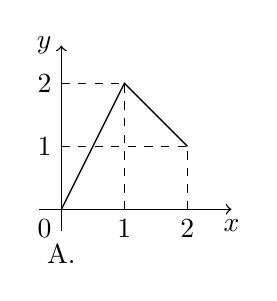
\begin{tikzpicture}[scale=0.8,line width=0.5pt]
\draw[->] (-0.35,0)--(2.7,0) node[below]{$x$};
\draw[->] (0,-0.35)--(0,2.6) node[left]{$y$};
\draw[dashed] (0,1)--(2,1) (0,2)--(1,2) (1,0)--(1,2) (2,0)--(2,1);
\draw (0,0)--(1,2)--(2,1);
\node[below left] at (0,0) {$0$};
\node[below] at (1,0) {$1$}; \node[below] at (2,0) {$2$};
\node[left] at (0,1) {$1$}; \node[left] at (0,2) {$2$};
\node[anchor=north] at (0,-0.4) {A.};
\end{tikzpicture}
&
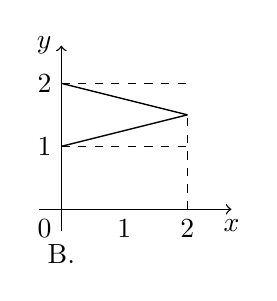
\begin{tikzpicture}[scale=0.8,line width=0.5pt]
\draw[->] (-0.35,0)--(2.7,0) node[below]{$x$};
\draw[->] (0,-0.35)--(0,2.6) node[left]{$y$};
\draw[dashed] (0,1)--(2,1) (0,2)--(2,2) (2,0)--(2,1.5);
\draw (0,2)--(2,1.5);
\draw (0,1)--(2,1.5);
\node[below left] at (0,0) {$0$};
\node[below] at (1,0) {$1$}; \node[below] at (2,0) {$2$};
\node[left] at (0,1) {$1$}; \node[left] at (0,2) {$2$};
\node[anchor=north] at (0,-0.4) {B.};
\end{tikzpicture}
\\[12pt]
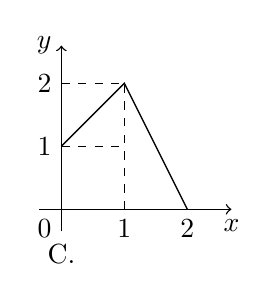
\begin{tikzpicture}[scale=0.8,line width=0.5pt]
\draw[->] (-0.35,0)--(2.7,0) node[below]{$x$};
\draw[->] (0,-0.35)--(0,2.6) node[left]{$y$};
\draw[dashed] (0,1)--(1,1) (0,2)--(1,2) (1,0)--(1,2);
\draw (0,1)--(1,2)--(2,0);
\node[below left] at (0,0) {$0$};
\node[below] at (1,0) {$1$}; \node[below] at (2,0) {$2$};
\node[left] at (0,1) {$1$}; \node[left] at (0,2) {$2$};
\node[anchor=north] at (0,-0.4) {C.};
\end{tikzpicture}
&
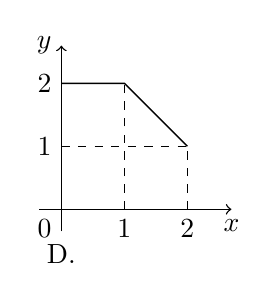
\begin{tikzpicture}[scale=0.8,line width=0.5pt]
\draw[->] (-0.35,0)--(2.7,0) node[below]{$x$};
\draw[->] (0,-0.35)--(0,2.6) node[left]{$y$};
\draw[dashed] (0,1)--(2,1) (1,0)--(1,2) (2,0)--(2,1);
\draw (0,2)--(1,2)--(2,1);
\node[below left] at (0,0) {$0$};
\node[below] at (1,0) {$1$}; \node[below] at (2,0) {$2$};
\node[left] at (0,1) {$1$}; \node[left] at (0,2) {$2$};
\node[anchor=north] at (0,-0.4) {D.};
\end{tikzpicture}
\end{tabular}
\end{center}

\ifanswer
\solbegin
\step{对于 $A$，当 $0\leqslant x\leqslant2$ 时，$0\leqslant y\leqslant2$，故 $A$ 错误；}
\step{对于 $B$，当 $0\leqslant x\leqslant2$ 时，任取一个 $x$ 的值，有两个 $y$ 与之对应，故 $B$ 错误；}
\step{对于 $C$，当 $0\leqslant x\leqslant2$ 时，$0\leqslant y\leqslant2$，故 $C$ 错误；}
\step{对于 $D$，当 $0\leqslant x\leqslant2$ 时，$0\leqslant y\leqslant2$，故 $D$ 正确.}
\step{故选 $D$.}
\solend
\fi

\item 下列函数中与函数 $y=x$ 是同一函数的是\mbox{（\quad）}

\keepwithprev
A. $y=\sqrt{x^2}$\qquad\quad B. $y=(\sqrt x)^2$\qquad\quad C. $u=\dfrac{v^2}{v}$\qquad\quad D. $m=\sqrt[5]{n^5}$

\ifanswer
\solbegin
\step{对于 $A$，$y=\sqrt{x^2}=\lvert x\rvert$，与函数 $y=x$ 的对应关系不相同，不是同一函数；}
\step{对于 $B$，$y=(\sqrt x)^2=x(x\geqslant0)$，与函数 $y=x(x\in\R)$ 的定义域不相同，不是同一函数；}
\step{对于 $C$，$u=\dfrac{v^2}{v}=v(v\neq0)$，与函数 $y=x(x\in\R)$ 的定义域不相同，不是同一函数；}
\step{对于 $D$，$m=\sqrt[5]{n^5}=n(n\in\R)$，与函数 $y=x(x\in\R)$ 的定义域相同，对应关系也相同，是同一函数.}
\step{故选 $D$.}
\solend
\fi

\item 某校高一四班学生 $46$ 人，寒假参加体育训练，其中足球队 $25$ 人，排球队 $22$ 人，游泳队 $24$ 人，足球排球都参加的有 $12$ 人，足球游泳都参加的有 $9$ 人，排球游泳都参加的有 $8$ 人，问：三项都参加的学生数为\mbox{（\quad）}

\keepwithprev
A. $2$\qquad\qquad B. $3$\qquad\qquad C. $4$\qquad\qquad D. $5$

\ifanswer
\solbegin
\step{设集合 $A=\{$参加足球队的学生$\}$，集合 $B=\{$参加排球队的学生$\}$，}
\step{集合 $C=\{$参加游泳队的学生$\}$，}
\step{则 $\operatorname{card}(A)=25$，$\operatorname{card}(B)=22$，$\operatorname{card}(C)=24$，}
\step{$\operatorname{card}(A\cap B)=12$，$\operatorname{card}(A\cap C)=9$，$\operatorname{card}(B\cap C)=8$，}
\step{设三项都参加的有 $x$ 人，即 $\operatorname{card}(A\cap B\cap C)=x$，$\operatorname{card}(A\cup B\cup C)=46$，}
\step{由 $\operatorname{card}(A\cup B\cup C)=\operatorname{card}A+\operatorname{card}B+\operatorname{card}C-\operatorname{card}(A\cap B)$}
\step{$-\operatorname{card}(B\cap C)-\operatorname{card}(A\cap C)+\operatorname{card}(A\cap B\cap C)$，}
\step{即 $46=25+22+24-12-8-9+x$，解得 $x=4$，所以三项都参加的有 $4$ 人.}
\step{故选 $C$.}
\solend
\fi

\item 已知 $\lg a$、$\lg b$ 是方程 $6x^2-4x-3=0$ 的两根，则 $\left(\lg\dfrac ab\right)^2$ 等于\mbox{（\quad）}

\keepwithprev
A. $\dfrac49$\qquad\qquad B. $\dfrac{13}{9}$\qquad\qquad C. $\dfrac{14}{9}$\qquad\qquad D. $\dfrac{22}{9}$

\ifanswer
\solbegin
\step{由韦达定理得 $\lg a+\lg b=\dfrac23$，$\lg a\cdot\lg b=-\dfrac12$，}
\step{所以 $\left(\lg\dfrac ab\right)^2=(\lg a-\lg b)^2=(\lg a+\lg b)^2-4\lg a\lg b=\dfrac49+2=\dfrac{22}{9}$. 故选 $D$.}
\solend
\fi

\end{enumerate}

\bigsec{三、解答题}

\begin{enumerate}
\setcounter{enumi}{16}

\item （1）用分数指数幂表示 $\sqrt[3]{a^2}\cdot\sqrt{a^3}$；

（2）已知 $a^{\frac12}+a^{-\frac12}=3$，求 $a+a^{-1}$.

\ifanswer
\solbegin
\step{（1）$\sqrt[3]{a^2}\cdot\sqrt{a^3}=a^{\frac23}\times a^{\frac32}=a^{\frac{13}6}$.}
\step{（2）由 $a^{\frac12}+a^{-\frac12}=3$，平方得 $a+2+a^{-1}=9$，故 $a+a^{-1}=7$.}
\solend
\fi

\item 已知 $f(x)=\begin{cases}x,x>0\\-x^2-2x+1,x\leqslant0\end{cases}$.

（1）求 $f(f(-2))$ 的值；

（2）若 $f(x_0)=2$，求 $x_0$ 的值.

\ifanswer
\solbegin
\step{（1）$f(x)=\begin{cases}x,x>0\\-x^2-2x+1,x\leqslant0\end{cases}$，则 $f(-2)=-(-2)^2-2\times(-2)+1=1$，}
\step{则有 $f(f(-2))=f(1)=1$；}
\step{（2）当 $x_0>0$ 时，$f(x_0)=x_0$，又 $f(x_0)=2$，所以 $x_0=2$，}
\step{当 $x_0\leqslant0$ 时，$f(x_0)=-x_0^2-2x_0+1$，又 $f(x_0)=2$，}
\step{所以 $-x_0^2-2x_0+1=2$，故 $x_0=-1$，}
\step{综上，$x_0$ 的值为 $-1$ 或 $2$.}
\solend
\fi

\item 已知集合 $A=\{x\mid\lvert 1+x\rvert+\lvert x\rvert<5\}$，$B=\left\{x\,\middle\vert\,\dfrac2{x-m}\geqslant1\right\}$，$p:x\in A$，$q:x\in B$.

（1）若 $m=0$，且 $p$ 真 $q$ 假，求实数 $x$ 的取值范围；

（2）若 $q$ 是 $p$ 的充分不必要条件，求实数 $m$ 的取值范围.

\ifanswer
\solbegin
\step{（1）当 $x\geqslant0$ 时，不等式 $\lvert 1+x\rvert+\lvert x\rvert<5$ 化为 $1+x+x<5$，解得 $0\leqslant x<2$；}
\step{当 $-1\leqslant x<0$ 时，不等式 $\lvert 1+x\rvert+\lvert x\rvert<5$ 化为 $1+x-x<5$ 恒成立，}
\step{故 $-1\leqslant x<0$；}
\step{当 $x<-1$ 时，不等式 $\lvert 1+x\rvert+\lvert x\rvert<5$ 化为 $-1-x-x<5$，}
\step{解得 $-3<x<-1$.}
\step{综上所述，$\lvert 1+x\rvert+\lvert x\rvert<5$ 等价于 $-3<x<2$，}
\step{所以 $\lvert 1+x\rvert+\lvert x\rvert<5$ 的解集为 $A=(-3,2)$，}
\step{若 $m=0$，则 $B=\left\{x\,\middle\vert\,\dfrac2x\geqslant1\right\}=\{x\mid 0<x\leqslant2\}$，得 $\overline{B}=(-\infty,0]\cup(2,+\infty)$，}
\step{由 $p$ 真 $q$ 假，得 $x\in(A\cap\overline{B})=(-3,0]$，即 $x$ 的取值范围为 $(-3,0]$；}
\step{（2）由 $\dfrac2{x-m}\geqslant1$，得 $\begin{cases}x-m>0\\x-m\leqslant2\end{cases}$，解得 $m<x\leqslant m+2$，}
\step{所以 $B=\left\{x\,\middle\vert\,\dfrac2{x-m}\geqslant1\right\}=(m,m+2]$，}
\step{由（1）的结论，得 $A=(-3,2)$，}
\step{若 $q$ 是 $p$ 的充分不必要条件，则 $B$ 是 $A$ 的真子集，得 $\begin{cases}m\geqslant-3\\m+2<2\end{cases}$，}
\step{解得 $-3\leqslant m<0$，即实数 $m$ 的取值范围是 $[-3,0)$.}
\solend
\fi

\item 某企业计划在 $2026$ 年布局人工智能大模型应用开发，生产智能终端配套的 $AI$ 算法服务包. 通过市场分析，全年需投入固定成本 $260$ 万元（含研发、服务器部署等），每生产 $x$ 千个算法服务包，需另投入成本 $R(x)$ 万元，且
$R(x)=\begin{cases}10x^2+100x,0<x\leqslant40\\601x+\dfrac{10000}{x}-7260,x>40\end{cases}$. 已知每个算法服务包的售价为 $0.6$ 万元，假设年内生产的服务包当年能全部销售完.

（1）试写出 $2026$ 年利润 $L$（万元）关于年产量 $x$（千个）的函数解析式；

（2）当 $2026$ 年产量为多少千个时，企业所获利润最大？并求出最大利润.

\ifanswer
\solbegin
\step{（1）$L(x)=x\cdot1000\times0.6-R(x)-260=600x-R(x)-260$，}
\step{当 $0<x\leqslant40$ 时，}
\step{$L(x)=600x-(10x^2+100x)-260=-10x^2+500x-260$；}
\step{当 $x>40$ 时，}
\step{$L(x)=600x-\left(601x+\dfrac{10000}{x}-7260\right)-260=7000-x-\dfrac{10000}{x}$；}
\step{综上，$L(x)=\begin{cases}-10x^2+500x-260,0<x\leqslant40\\7000-x-\dfrac{10000}{x},x>40\end{cases}$；}
\step{（2）当 $0<x\leqslant40$ 时，$L(x)=-10x^2+500x-260=-10(x-25)^2+5990$，}
\step{当 $x=25$ 时，函数 $L(x)$ 有最大值 $5990$；}
\step{当 $x>40$ 时，$L(x)=7000-x-\dfrac{10000}{x}=7000-\left(x+\dfrac{10000}{x}\right)$}
\step{$\leqslant7000-2\sqrt{x\cdot\dfrac{10000}{x}}=7000-2\times100=6800$，}
\step{当且仅当 $x=\dfrac{10000}{x}$ 时取等号，}
\step{所以当 $x=100$ 时，函数 $L(x)$ 有最大值 $6800$；}
\step{因为 $6800>5990$，所以 $2026$ 年产量为 $100$ 千个时，企业所获利润最大，}
\step{最大利润为 $6800$ 万元.}
\solend
\fi

\item 已知二次函数 $f(x)=ax^2+bx+c$.

（1）若 $f(x)>0$ 的解集为 $\{x\mid-3<x<4\}$，解关于 $x$ 的不等式 $bx^2+2ax-(c+3b)<0$；

（2）若函数满足 $f(x+1)-f(x)=2x+2$，且 $f(0)=1$. 求 $f(x)$ 的解析式；

（3）若对任意 $x\in\R$，不等式 $f(x)\geqslant2ax+b$ 恒成立，求 $\dfrac{b^2}{4(a^2+c^2)}$ 的最大值.

\ifanswer
\solbegin
\step{（1）由题意二次函数 $f(x)=ax^2+bx+c$，}
\step{若 $f(x)>0$ 的解集为 $\{x\mid-3<x<4\}$，}
\step{得 $-3$、$4$ 为方程 $ax^2+bx+c=0$ 的根，且 $a<0$，}
\step{则 $\begin{cases}-3+4=-\dfrac ba\\-3\times4=\dfrac ca\end{cases}$，即 $b=-a$，$c=-12a$，}
\step{则不等式 $bx^2+2ax-(c+3b)<0$，即为 $-ax^2+2ax+15a<0(a<0)$，}
\step{则 $x^2-2x-15<0$，解得 $-3<x<5$，}
\step{所以不等式 $bx^2+2ax-(c+3b)<0$ 的解集为 $(-3,5)$；}
\step{（2）由 $f(x)=ax^2+bx+c(a\neq0)$，}
\step{则 $f(x+1)-f(x)=a(x+1)^2+b(x+1)+c-(ax^2+bx+c)=2ax+a+b$，}
\step{又 $f(x+1)-f(x)=2x+2$，故 $\begin{cases}2a=2\\a+b=2\end{cases}$，解得 $a=1$，$b=1$，}
\step{由 $f(0)=1$，得 $c=1$，所以 $f(x)=x^2+x+1$；}
\step{（3）由题意二次函数 $f(x)=ax^2+bx+c$，}
\step{若对任意 $x\in\R$，不等式 $f(x)\geqslant2ax+b$ 恒成立，}
\step{得对任意 $x\in\R$，$ax^2+bx+c\geqslant2ax+b$ 恒成立，}
\step{整理得 $ax^2+(b-2a)x+c-b\geqslant0$ 恒成立，}
\step{因为 $a$ 不为 $0$，所以 $\begin{cases}a>0\\\Delta=(b-2a)^2-4a(c-b)\leqslant0\end{cases}$，}
\step{所以 $0\leqslant b^2\leqslant4a(c-a)$，所以 $\dfrac{b^2}{4(a^2+c^2)}\leqslant\dfrac{ac-a^2}{a^2+c^2}=\dfrac{\frac ca-1}{1+\left(\frac ca\right)^2}$，}
\step{令 $t=\dfrac ca-1$，因为 $0\leqslant b^2\leqslant4a(c-a)$，所以 $c\geqslant a>0\Rightarrow t\geqslant0$，}
\step{若 $t=0$ 时，此时 $\dfrac{b^2}{4(a^2+c^2)}\leqslant\dfrac{\frac ca-1}{1+\left(\frac ca\right)^2}=0$，}
\step{若 $t>0$ 时，$\dfrac{b^2}{4(a^2+c^2)}\leqslant\dfrac{t}{1+(t+1)^2}=\dfrac{t}{t^2+2t+2}=\dfrac1{t+\frac2t+2}$}
\step{$\leqslant\dfrac1{2\sqrt2+2}=\dfrac{\sqrt2-1}{2}$，}
\step{当且仅当 $t=\dfrac2t$，即 $t=\sqrt2$ 时，即 $c=(1+\sqrt2)a$ 时，上式取等号.}
\step{综上所述，$\dfrac{b^2}{4(a^2+c^2)}$ 的最大值为 $\dfrac{\sqrt2-1}{2}$.}
\solend
\fi

\end{enumerate}

\end{document}
"
%
% 原始材料：微信公众号“魔都数学加油站”文章，作者破晓，2026-11-06 17:58 发布；
% 连载“27学年高一117”，原文标题“27学年高一117——2026-2027年上海市陆行中学高一上期中”；
% 原文链接：https://mp.weixin.qq.com/s/of8iPW26dvDyXWohudT0vw。
% 正文为 10 张 PNG 页（第 1、3、4、8、9、10 页 2560×3620，其余 4762×6735），
% 题目下印有【解析】或【答案】，为讲评版。
% 题目、解析均据原图转录；卷面红色水印及公众号页脚未录入。
%
% 卷首标题：原卷印作“2026-2027 年陆行中学高一上期中”（公众号标题中的“上海市”
% 卷面标题行没有，本稿照卷面），年份区间按全稿惯例排 en dash；原卷未印副标题，本稿按题目内容
% 标为“集合与常用逻辑用语、不等式、函数”（期中卷跨三章，含指数／对数与函数，与 112 同）。
%
% 与原卷的排版差异：
%   ① 原文从第 3 题起，填空题 3—12、选择题 13—16、解答题 17—21，共 19 题，本稿保留原题号；
%   ② 原卷每题下直接印【解析】／【答案】，本稿按全稿惯例置于答案版；第 4、6、8 题只印
%      【答案】，另提 \ans{}；其余选择题答案在解析末句“故选 …”，括号内留空；
%   ③ 原卷未印副标题，本稿按“知识模块”口径补出；
%   ④ 原卷填空横线按全稿惯例排为 \blankline[4.4em]；选择题括号排 \mbox{（\quad）}、
%      选项段前按惯例加 \keepwithprev；解答题不留作答区（原卷为讲评版，与 109—116 同）；
%   ⑤ 原卷 $max$／$min$ 排斜体，按 96 成例改 \max／\min；数集 $R$ 按惯例改 \R。
%
% 判别式字形：第 11 题与第 21 题 (3) 的判别式原卷排 $\Delta$（等腰、右厚），照录 \Delta。
%
% 子集符号：第 5 题的 $B\subseteq A$ 印有下划线，照录 \subseteq。
%
% 第 13 题四个坐标图选项按原图形状用 TikZ 重排（三版都出）；原卷另有第 12 题的
%   $a\odot b$ 自定义运算、第 15 题的 $\operatorname{card}$ 记号，均照录。
%
% 原卷存疑照录：第 12 题解析的 $\min\{\left|x\right|\odot\left|3-x\right|\}$ 一行、
%   第 20 题 $R(x)$ 分段函数与 $L(x)$ 的推导，均按原卷印刷行照录。
%   第 20 题题干开头原卷有一段会议背景引语（非数学信息），本稿从“某企业计划在
%   $2026$ 年布局…”起照录题目主体，全部数据、设问与解析均完整保留。
%
% 行数核对：逐题数 \step/\stepm 条数，合计 106 条（Q3：1；Q4：0；Q5：5；Q6：0；Q7：3；
% Q8：0；Q9：3；Q10：3；Q11：5；Q12：6；Q13：5；Q14：5；Q15：9；Q16：2；Q17：2；
% Q18：6；Q19：14；Q20：14；Q21：23），与原卷印刷行逐题相等（cases／TikZ 图块作一个
% 印刷行计）。第 4、6、8 题只印【答案】，提 \ans{}，不计入 \step 账。
%
\documentclass[a4paper,11pt]{article}
\usepackage{common}

\begin{document}

\examtitlest[3]{2026--2027 年陆行中学高一上期中}{集合与常用逻辑用语、不等式、函数}

\bigsec{一、填空题}

\begin{enumerate}
\setcounter{enumi}{2}

\item 已知 $10^a=2$,$10^b=5$，则 $10^{3a-2b}$ 的值为\blankline[4.4em].

\ifanswer
\solbegin
\step{$10^{3a-2b}=\dfrac{10^{3a}}{10^{2b}}=\dfrac{(10^a)^3}{(10^b)^2}=\dfrac{2^3}{5^2}=\dfrac8{25}$.}
\solend
\fi

\item 已知不等式 $\lvert x+1\rvert+\lvert x-3\rvert\geqslant4$ 恒成立，则取等号时 $x$ 的取值范围是\blankline[4.4em].

\ifanswer
\ans{$[-1,3]$}
\fi

\item 集合 $A=\{1,2,a^2\}$，$B=\{2,a\}$，若 $B\subseteq A$，则 $a$ 的值为\blankline[4.4em].

\ifanswer
\solbegin
\step{因为 $B\subseteq A$，所以 $a=1$ 或 $a=a^2$，}
\step{当 $a=1$ 时，$a^2=1$，不满足元素的互异性，故舍去；}
\step{当 $a=a^2$ 时，解得 $a=1$（舍）或 $a=0$，}
\step{当 $a=0$ 时，$A=\{1,2,0\}$，$B=\{2,0\}$，满足题意.}
\step{综上，$a=0$.}
\solend
\fi

\item 若 $x>\dfrac35$，则 $y=5x+\dfrac1{5x-3}$ 的最小值是\blankline[4.4em].

\ifanswer
\ans{$5$}
\fi

\item 已知 $a>0$，$b>0$，且 $a+b=1$，则 $\dfrac3a+\dfrac1b$ 的最小值是\blankline[4.4em].

\ifanswer
\solbegin
\step{$a>0$，$b>0$，且 $a+b=1$，}
\step{$\dfrac3a+\dfrac1b=\left(\dfrac3a+\dfrac1b\right)(a+b)=\dfrac{3b}{a}+\dfrac ab+4\geqslant2\sqrt3+4$，}
\step{当且仅当 $\dfrac{3b}{a}=\dfrac ab$ 时取等号，所以 $\dfrac3a+\dfrac1b$ 的最小值为 $2\sqrt3+4$.}
\solend
\fi

\item 已知 $\log_2 5=a$，则 $\log_5 10=$\blankline[4.4em]（用含 $a$ 的代数式表示）.

\ifanswer
\ans{$1+\dfrac1a$}
\fi

\item 已知 $p:2<x\leqslant3$，$q:\lvert x-a\rvert<2$，若 $p$ 是 $q$ 的充分不必要条件，则实数 $a$ 的取值范围为\blankline[4.4em].

\ifanswer
\solbegin
\step{由 $\lvert x-a\rvert<2$ 得 $a-2<x<a+2$，即 $p:2<x\leqslant3$，$q:a-2<x<a+2$.}
\step{因为 $p$ 是 $q$ 的充分不必要条件，所以 $\begin{cases}a-2\leqslant2\\a+2>3\end{cases}$，解得 $1<a\leqslant4$，}
\step{所以实数 $a$ 的取值范围为 $(1,4]$.}
\solend
\fi

\item 已知 $a>1$,$b>1$，若 $\log_a b+\log_b a=2$，且 $ab=2$，则 $\log_2(a+b)=$\blankline[4.4em].

\ifanswer
\solbegin
\step{由 $\log_a b+\log_b a=2$,$a>1$,$b>1$，得 $\log_a b+\dfrac1{\log_a b}=2$，}
\step{即 $(\log_a b)^2-2\log_a b+1=0$，则 $(\log_a b-1)^2=0$，即 $\log_a b=1$，则 $a=b$，}
\step{又 $ab=2$，则 $a=b=\sqrt2$，所以 $\log_2(a+b)=\log_2(2\sqrt2)=\log_2 2^{\frac32}=\dfrac32$.}
\solend
\fi

\item 已知函数 $f(x)=\sqrt{2kx^2+kx+\dfrac34}$ 的定义域为实数集 $\R$，则实数 $k$ 的取值范围\blankline[4.4em].

\ifanswer
\solbegin
\step{因为函数 $f(x)=\sqrt{2kx^2+kx+\dfrac34}$ 的定义域为实数集 $\R$，}
\step{所以 $2kx^2+kx+\dfrac34\geqslant0$ 在 $\R$ 上恒成立，}
\step{当 $k=0$ 时，$\dfrac34\geqslant0$，恒成立；}
\step{当 $k\neq0$ 时，则有 $\begin{cases}2k>0\\\Delta=k^2-4\times2k\times\dfrac34\leqslant0\end{cases}$，解得 $0<k\leqslant6$；}
\step{综上，实数 $k$ 的取值范围为 $[0,6]$.}
\solend
\fi

\item 对于两个实数 $a$、$b$，定义运算 $a\odot b$ 如下：若 $a\geqslant b$，则 $a\odot b=a$；若 $a<b$，则 $a\odot b=b$. 若 $x$、$y\in\R$，则 $\lvert x-y\rvert\odot\lvert 3-x\rvert\odot\lvert x+y\rvert$ 的最小值是\blankline[4.4em].

\ifanswer
\solbegin
\step{由题意得 $a\odot b=\max\{a,b\}$，所以 $\lvert a+b\rvert\odot\lvert a-b\rvert=\max\{\lvert a+b\rvert,\lvert a-b\rvert\}$，}
\step{设 $\max\{\lvert a+b\rvert,\lvert a-b\rvert\}=M$，则 $\begin{cases}M\geqslant\lvert a+b\rvert\\M\geqslant\lvert a-b\rvert\end{cases}$，}
\step{所以 $2M\geqslant\lvert a+b\rvert+\lvert a-b\rvert\geqslant2\lvert a\rvert$，则 $\lvert a+b\rvert\odot\lvert a-b\rvert\geqslant\lvert a\rvert$，}
\step{所以 $\min\{\lvert x-y\rvert\odot\lvert 3-x\rvert\odot\lvert x+y\rvert\}=\min\{\lvert x-y\rvert\odot\lvert x+y\rvert\odot\lvert 3-x\rvert\}$}
\step{$=\min\{\lvert x\rvert\odot\lvert 3-x\rvert\}=\min\left\{\dfrac32+x\odot\left\lvert\dfrac32-x\right\rvert\right\}=\dfrac32$，}% 原卷该行写法照录
\step{当且仅当 $x=\dfrac32$，$y=0$ 取等号，故 $\lvert x-y\rvert\odot\lvert 3-x\rvert\odot\lvert x+y\rvert$ 的最小值是 $\dfrac32$.}
\solend
\fi

\end{enumerate}

\bigsec{二、选择题}

\begin{enumerate}
\setcounter{enumi}{12}

\item 设 $A=\{x\mid 0\leqslant x\leqslant2\}$，$B=\{y\mid 1\leqslant y\leqslant2\}$，下列图形能表示从集合 $A$ 到集合 $B$ 的函数图像的是\mbox{（\quad）}

\keepwithprev
\begin{center}
% 原卷四个坐标图选项按原图形状用 TikZ 重排。
\begin{tabular}{c@{\qquad\qquad}c}
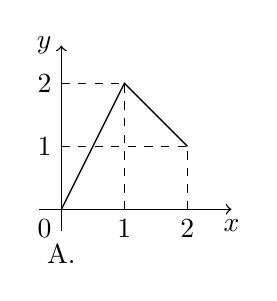
\begin{tikzpicture}[scale=0.8,line width=0.5pt]
\draw[->] (-0.35,0)--(2.7,0) node[below]{$x$};
\draw[->] (0,-0.35)--(0,2.6) node[left]{$y$};
\draw[dashed] (0,1)--(2,1) (0,2)--(1,2) (1,0)--(1,2) (2,0)--(2,1);
\draw (0,0)--(1,2)--(2,1);
\node[below left] at (0,0) {$0$};
\node[below] at (1,0) {$1$}; \node[below] at (2,0) {$2$};
\node[left] at (0,1) {$1$}; \node[left] at (0,2) {$2$};
\node[anchor=north] at (0,-0.4) {A.};
\end{tikzpicture}
&
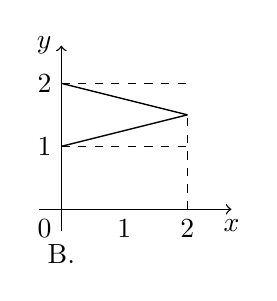
\begin{tikzpicture}[scale=0.8,line width=0.5pt]
\draw[->] (-0.35,0)--(2.7,0) node[below]{$x$};
\draw[->] (0,-0.35)--(0,2.6) node[left]{$y$};
\draw[dashed] (0,1)--(2,1) (0,2)--(2,2) (2,0)--(2,1.5);
\draw (0,2)--(2,1.5);
\draw (0,1)--(2,1.5);
\node[below left] at (0,0) {$0$};
\node[below] at (1,0) {$1$}; \node[below] at (2,0) {$2$};
\node[left] at (0,1) {$1$}; \node[left] at (0,2) {$2$};
\node[anchor=north] at (0,-0.4) {B.};
\end{tikzpicture}
\\[12pt]
\begin{tikzpicture}[scale=0.8,line width=0.5pt]
\draw[->] (-0.35,0)--(2.7,0) node[below]{$x$};
\draw[->] (0,-0.35)--(0,2.6) node[left]{$y$};
\draw[dashed] (0,1)--(1,1) (0,2)--(1,2) (1,0)--(1,2);
\draw (0,1)--(1,2)--(2,0);
\node[below left] at (0,0) {$0$};
\node[below] at (1,0) {$1$}; \node[below] at (2,0) {$2$};
\node[left] at (0,1) {$1$}; \node[left] at (0,2) {$2$};
\node[anchor=north] at (0,-0.4) {C.};
\end{tikzpicture}
&
\begin{tikzpicture}[scale=0.8,line width=0.5pt]
\draw[->] (-0.35,0)--(2.7,0) node[below]{$x$};
\draw[->] (0,-0.35)--(0,2.6) node[left]{$y$};
\draw[dashed] (0,1)--(2,1) (1,0)--(1,2) (2,0)--(2,1);
\draw (0,2)--(1,2)--(2,1);
\node[below left] at (0,0) {$0$};
\node[below] at (1,0) {$1$}; \node[below] at (2,0) {$2$};
\node[left] at (0,1) {$1$}; \node[left] at (0,2) {$2$};
\node[anchor=north] at (0,-0.4) {D.};
\end{tikzpicture}
\end{tabular}
\end{center}

\ifanswer
\solbegin
\step{对于 $A$，当 $0\leqslant x\leqslant2$ 时，$0\leqslant y\leqslant2$，故 $A$ 错误；}
\step{对于 $B$，当 $0\leqslant x\leqslant2$ 时，任取一个 $x$ 的值，有两个 $y$ 与之对应，故 $B$ 错误；}
\step{对于 $C$，当 $0\leqslant x\leqslant2$ 时，$0\leqslant y\leqslant2$，故 $C$ 错误；}
\step{对于 $D$，当 $0\leqslant x\leqslant2$ 时，$0\leqslant y\leqslant2$，故 $D$ 正确.}
\step{故选 $D$.}
\solend
\fi

\item 下列函数中与函数 $y=x$ 是同一函数的是\mbox{（\quad）}

\keepwithprev
A. $y=\sqrt{x^2}$\qquad\quad B. $y=(\sqrt x)^2$\qquad\quad C. $u=\dfrac{v^2}{v}$\qquad\quad D. $m=\sqrt[5]{n^5}$

\ifanswer
\solbegin
\step{对于 $A$，$y=\sqrt{x^2}=\lvert x\rvert$，与函数 $y=x$ 的对应关系不相同，不是同一函数；}
\step{对于 $B$，$y=(\sqrt x)^2=x(x\geqslant0)$，与函数 $y=x(x\in\R)$ 的定义域不相同，不是同一函数；}
\step{对于 $C$，$u=\dfrac{v^2}{v}=v(v\neq0)$，与函数 $y=x(x\in\R)$ 的定义域不相同，不是同一函数；}
\step{对于 $D$，$m=\sqrt[5]{n^5}=n(n\in\R)$，与函数 $y=x(x\in\R)$ 的定义域相同，对应关系也相同，是同一函数.}
\step{故选 $D$.}
\solend
\fi

\item 某校高一四班学生 $46$ 人，寒假参加体育训练，其中足球队 $25$ 人，排球队 $22$ 人，游泳队 $24$ 人，足球排球都参加的有 $12$ 人，足球游泳都参加的有 $9$ 人，排球游泳都参加的有 $8$ 人，问：三项都参加的学生数为\mbox{（\quad）}

\keepwithprev
A. $2$\qquad\qquad B. $3$\qquad\qquad C. $4$\qquad\qquad D. $5$

\ifanswer
\solbegin
\step{设集合 $A=\{$参加足球队的学生$\}$，集合 $B=\{$参加排球队的学生$\}$，}
\step{集合 $C=\{$参加游泳队的学生$\}$，}
\step{则 $\operatorname{card}(A)=25$，$\operatorname{card}(B)=22$，$\operatorname{card}(C)=24$，}
\step{$\operatorname{card}(A\cap B)=12$，$\operatorname{card}(A\cap C)=9$，$\operatorname{card}(B\cap C)=8$，}
\step{设三项都参加的有 $x$ 人，即 $\operatorname{card}(A\cap B\cap C)=x$，$\operatorname{card}(A\cup B\cup C)=46$，}
\step{由 $\operatorname{card}(A\cup B\cup C)=\operatorname{card}A+\operatorname{card}B+\operatorname{card}C-\operatorname{card}(A\cap B)$}
\step{$-\operatorname{card}(B\cap C)-\operatorname{card}(A\cap C)+\operatorname{card}(A\cap B\cap C)$，}
\step{即 $46=25+22+24-12-8-9+x$，解得 $x=4$，所以三项都参加的有 $4$ 人.}
\step{故选 $C$.}
\solend
\fi

\item 已知 $\lg a$、$\lg b$ 是方程 $6x^2-4x-3=0$ 的两根，则 $\left(\lg\dfrac ab\right)^2$ 等于\mbox{（\quad）}

\keepwithprev
A. $\dfrac49$\qquad\qquad B. $\dfrac{13}{9}$\qquad\qquad C. $\dfrac{14}{9}$\qquad\qquad D. $\dfrac{22}{9}$

\ifanswer
\solbegin
\step{由韦达定理得 $\lg a+\lg b=\dfrac23$，$\lg a\cdot\lg b=-\dfrac12$，}
\step{所以 $\left(\lg\dfrac ab\right)^2=(\lg a-\lg b)^2=(\lg a+\lg b)^2-4\lg a\lg b=\dfrac49+2=\dfrac{22}{9}$. 故选 $D$.}
\solend
\fi

\end{enumerate}

\bigsec{三、解答题}

\begin{enumerate}
\setcounter{enumi}{16}

\item （1）用分数指数幂表示 $\sqrt[3]{a^2}\cdot\sqrt{a^3}$；

（2）已知 $a^{\frac12}+a^{-\frac12}=3$，求 $a+a^{-1}$.

\ifanswer
\solbegin
\step{（1）$\sqrt[3]{a^2}\cdot\sqrt{a^3}=a^{\frac23}\times a^{\frac32}=a^{\frac{13}6}$.}
\step{（2）由 $a^{\frac12}+a^{-\frac12}=3$，平方得 $a+2+a^{-1}=9$，故 $a+a^{-1}=7$.}
\solend
\fi

\item 已知 $f(x)=\begin{cases}x,x>0\\-x^2-2x+1,x\leqslant0\end{cases}$.

（1）求 $f(f(-2))$ 的值；

（2）若 $f(x_0)=2$，求 $x_0$ 的值.

\ifanswer
\solbegin
\step{（1）$f(x)=\begin{cases}x,x>0\\-x^2-2x+1,x\leqslant0\end{cases}$，则 $f(-2)=-(-2)^2-2\times(-2)+1=1$，}
\step{则有 $f(f(-2))=f(1)=1$；}
\step{（2）当 $x_0>0$ 时，$f(x_0)=x_0$，又 $f(x_0)=2$，所以 $x_0=2$，}
\step{当 $x_0\leqslant0$ 时，$f(x_0)=-x_0^2-2x_0+1$，又 $f(x_0)=2$，}
\step{所以 $-x_0^2-2x_0+1=2$，故 $x_0=-1$，}
\step{综上，$x_0$ 的值为 $-1$ 或 $2$.}
\solend
\fi

\item 已知集合 $A=\{x\mid\lvert 1+x\rvert+\lvert x\rvert<5\}$，$B=\left\{x\,\middle\vert\,\dfrac2{x-m}\geqslant1\right\}$，$p:x\in A$，$q:x\in B$.

（1）若 $m=0$，且 $p$ 真 $q$ 假，求实数 $x$ 的取值范围；

（2）若 $q$ 是 $p$ 的充分不必要条件，求实数 $m$ 的取值范围.

\ifanswer
\solbegin
\step{（1）当 $x\geqslant0$ 时，不等式 $\lvert 1+x\rvert+\lvert x\rvert<5$ 化为 $1+x+x<5$，解得 $0\leqslant x<2$；}
\step{当 $-1\leqslant x<0$ 时，不等式 $\lvert 1+x\rvert+\lvert x\rvert<5$ 化为 $1+x-x<5$ 恒成立，}
\step{故 $-1\leqslant x<0$；}
\step{当 $x<-1$ 时，不等式 $\lvert 1+x\rvert+\lvert x\rvert<5$ 化为 $-1-x-x<5$，}
\step{解得 $-3<x<-1$.}
\step{综上所述，$\lvert 1+x\rvert+\lvert x\rvert<5$ 等价于 $-3<x<2$，}
\step{所以 $\lvert 1+x\rvert+\lvert x\rvert<5$ 的解集为 $A=(-3,2)$，}
\step{若 $m=0$，则 $B=\left\{x\,\middle\vert\,\dfrac2x\geqslant1\right\}=\{x\mid 0<x\leqslant2\}$，得 $\overline{B}=(-\infty,0]\cup(2,+\infty)$，}
\step{由 $p$ 真 $q$ 假，得 $x\in(A\cap\overline{B})=(-3,0]$，即 $x$ 的取值范围为 $(-3,0]$；}
\step{（2）由 $\dfrac2{x-m}\geqslant1$，得 $\begin{cases}x-m>0\\x-m\leqslant2\end{cases}$，解得 $m<x\leqslant m+2$，}
\step{所以 $B=\left\{x\,\middle\vert\,\dfrac2{x-m}\geqslant1\right\}=(m,m+2]$，}
\step{由（1）的结论，得 $A=(-3,2)$，}
\step{若 $q$ 是 $p$ 的充分不必要条件，则 $B$ 是 $A$ 的真子集，得 $\begin{cases}m\geqslant-3\\m+2<2\end{cases}$，}
\step{解得 $-3\leqslant m<0$，即实数 $m$ 的取值范围是 $[-3,0)$.}
\solend
\fi

\item 某企业计划在 $2026$ 年布局人工智能大模型应用开发，生产智能终端配套的 $AI$ 算法服务包. 通过市场分析，全年需投入固定成本 $260$ 万元（含研发、服务器部署等），每生产 $x$ 千个算法服务包，需另投入成本 $R(x)$ 万元，且
$R(x)=\begin{cases}10x^2+100x,0<x\leqslant40\\601x+\dfrac{10000}{x}-7260,x>40\end{cases}$. 已知每个算法服务包的售价为 $0.6$ 万元，假设年内生产的服务包当年能全部销售完.

（1）试写出 $2026$ 年利润 $L$（万元）关于年产量 $x$（千个）的函数解析式；

（2）当 $2026$ 年产量为多少千个时，企业所获利润最大？并求出最大利润.

\ifanswer
\solbegin
\step{（1）$L(x)=x\cdot1000\times0.6-R(x)-260=600x-R(x)-260$，}
\step{当 $0<x\leqslant40$ 时，}
\step{$L(x)=600x-(10x^2+100x)-260=-10x^2+500x-260$；}
\step{当 $x>40$ 时，}
\step{$L(x)=600x-\left(601x+\dfrac{10000}{x}-7260\right)-260=7000-x-\dfrac{10000}{x}$；}
\step{综上，$L(x)=\begin{cases}-10x^2+500x-260,0<x\leqslant40\\7000-x-\dfrac{10000}{x},x>40\end{cases}$；}
\step{（2）当 $0<x\leqslant40$ 时，$L(x)=-10x^2+500x-260=-10(x-25)^2+5990$，}
\step{当 $x=25$ 时，函数 $L(x)$ 有最大值 $5990$；}
\step{当 $x>40$ 时，$L(x)=7000-x-\dfrac{10000}{x}=7000-\left(x+\dfrac{10000}{x}\right)$}
\step{$\leqslant7000-2\sqrt{x\cdot\dfrac{10000}{x}}=7000-2\times100=6800$，}
\step{当且仅当 $x=\dfrac{10000}{x}$ 时取等号，}
\step{所以当 $x=100$ 时，函数 $L(x)$ 有最大值 $6800$；}
\step{因为 $6800>5990$，所以 $2026$ 年产量为 $100$ 千个时，企业所获利润最大，}
\step{最大利润为 $6800$ 万元.}
\solend
\fi

\item 已知二次函数 $f(x)=ax^2+bx+c$.

（1）若 $f(x)>0$ 的解集为 $\{x\mid-3<x<4\}$，解关于 $x$ 的不等式 $bx^2+2ax-(c+3b)<0$；

（2）若函数满足 $f(x+1)-f(x)=2x+2$，且 $f(0)=1$. 求 $f(x)$ 的解析式；

（3）若对任意 $x\in\R$，不等式 $f(x)\geqslant2ax+b$ 恒成立，求 $\dfrac{b^2}{4(a^2+c^2)}$ 的最大值.

\ifanswer
\solbegin
\step{（1）由题意二次函数 $f(x)=ax^2+bx+c$，}
\step{若 $f(x)>0$ 的解集为 $\{x\mid-3<x<4\}$，}
\step{得 $-3$、$4$ 为方程 $ax^2+bx+c=0$ 的根，且 $a<0$，}
\step{则 $\begin{cases}-3+4=-\dfrac ba\\-3\times4=\dfrac ca\end{cases}$，即 $b=-a$，$c=-12a$，}
\step{则不等式 $bx^2+2ax-(c+3b)<0$，即为 $-ax^2+2ax+15a<0(a<0)$，}
\step{则 $x^2-2x-15<0$，解得 $-3<x<5$，}
\step{所以不等式 $bx^2+2ax-(c+3b)<0$ 的解集为 $(-3,5)$；}
\step{（2）由 $f(x)=ax^2+bx+c(a\neq0)$，}
\step{则 $f(x+1)-f(x)=a(x+1)^2+b(x+1)+c-(ax^2+bx+c)=2ax+a+b$，}
\step{又 $f(x+1)-f(x)=2x+2$，故 $\begin{cases}2a=2\\a+b=2\end{cases}$，解得 $a=1$，$b=1$，}
\step{由 $f(0)=1$，得 $c=1$，所以 $f(x)=x^2+x+1$；}
\step{（3）由题意二次函数 $f(x)=ax^2+bx+c$，}
\step{若对任意 $x\in\R$，不等式 $f(x)\geqslant2ax+b$ 恒成立，}
\step{得对任意 $x\in\R$，$ax^2+bx+c\geqslant2ax+b$ 恒成立，}
\step{整理得 $ax^2+(b-2a)x+c-b\geqslant0$ 恒成立，}
\step{因为 $a$ 不为 $0$，所以 $\begin{cases}a>0\\\Delta=(b-2a)^2-4a(c-b)\leqslant0\end{cases}$，}
\step{所以 $0\leqslant b^2\leqslant4a(c-a)$，所以 $\dfrac{b^2}{4(a^2+c^2)}\leqslant\dfrac{ac-a^2}{a^2+c^2}=\dfrac{\frac ca-1}{1+\left(\frac ca\right)^2}$，}
\step{令 $t=\dfrac ca-1$，因为 $0\leqslant b^2\leqslant4a(c-a)$，所以 $c\geqslant a>0\Rightarrow t\geqslant0$，}
\step{若 $t=0$ 时，此时 $\dfrac{b^2}{4(a^2+c^2)}\leqslant\dfrac{\frac ca-1}{1+\left(\frac ca\right)^2}=0$，}
\step{若 $t>0$ 时，$\dfrac{b^2}{4(a^2+c^2)}\leqslant\dfrac{t}{1+(t+1)^2}=\dfrac{t}{t^2+2t+2}=\dfrac1{t+\frac2t+2}$}
\step{$\leqslant\dfrac1{2\sqrt2+2}=\dfrac{\sqrt2-1}{2}$，}
\step{当且仅当 $t=\dfrac2t$，即 $t=\sqrt2$ 时，即 $c=(1+\sqrt2)a$ 时，上式取等号.}
\step{综上所述，$\dfrac{b^2}{4(a^2+c^2)}$ 的最大值为 $\dfrac{\sqrt2-1}{2}$.}
\solend
\fi

\end{enumerate}

\end{document}
"
%
% 原始材料：微信公众号“魔都数学加油站”文章，作者破晓，2026-11-06 17:58 发布；
% 连载“27学年高一117”，原文标题“27学年高一117——2026-2027年上海市陆行中学高一上期中”；
% 原文链接：https://mp.weixin.qq.com/s/of8iPW26dvDyXWohudT0vw。
% 正文为 10 张 PNG 页（第 1、3、4、8、9、10 页 2560×3620，其余 4762×6735），
% 题目下印有【解析】或【答案】，为讲评版。
% 题目、解析均据原图转录；卷面红色水印及公众号页脚未录入。
%
% 卷首标题：原卷印作“2026-2027 年陆行中学高一上期中”（公众号标题中的“上海市”
% 卷面标题行没有，本稿照卷面），年份区间按全稿惯例排 en dash；原卷未印副标题，本稿按题目内容
% 标为“集合与常用逻辑用语、不等式、函数”（期中卷跨三章，含指数／对数与函数，与 112 同）。
%
% 与原卷的排版差异：
%   ① 原文从第 3 题起，填空题 3—12、选择题 13—16、解答题 17—21，共 19 题，本稿保留原题号；
%   ② 原卷每题下直接印【解析】／【答案】，本稿按全稿惯例置于答案版；第 4、6、8 题只印
%      【答案】，另提 \ans{}；其余选择题答案在解析末句“故选 …”，括号内留空；
%   ③ 原卷未印副标题，本稿按“知识模块”口径补出；
%   ④ 原卷填空横线按全稿惯例排为 \blankline[4.4em]；选择题括号排 \mbox{（\quad）}、
%      选项段前按惯例加 \keepwithprev；解答题不留作答区（原卷为讲评版，与 109—116 同）；
%   ⑤ 原卷 $max$／$min$ 排斜体，按 96 成例改 \max／\min；数集 $R$ 按惯例改 \R。
%
% 判别式字形：第 11 题与第 21 题 (3) 的判别式原卷排 $\Delta$（等腰、右厚），照录 \Delta。
%
% 子集符号：第 5 题的 $B\subseteq A$ 印有下划线，照录 \subseteq。
%
% 第 13 题四个坐标图选项按原图形状用 TikZ 重排（三版都出）；原卷另有第 12 题的
%   $a\odot b$ 自定义运算、第 15 题的 $\operatorname{card}$ 记号，均照录。
%
% 原卷存疑照录：第 12 题解析的 $\min\{\left|x\right|\odot\left|3-x\right|\}$ 一行、
%   第 20 题 $R(x)$ 分段函数与 $L(x)$ 的推导，均按原卷印刷行照录。
%   第 20 题题干开头原卷有一段会议背景引语（非数学信息），本稿从“某企业计划在
%   $2026$ 年布局…”起照录题目主体，全部数据、设问与解析均完整保留。
%
% 行数核对：逐题数 \step/\stepm 条数，合计 106 条（Q3：1；Q4：0；Q5：5；Q6：0；Q7：3；
% Q8：0；Q9：3；Q10：3；Q11：5；Q12：6；Q13：5；Q14：5；Q15：9；Q16：2；Q17：2；
% Q18：6；Q19：14；Q20：14；Q21：23），与原卷印刷行逐题相等（cases／TikZ 图块作一个
% 印刷行计）。第 4、6、8 题只印【答案】，提 \ans{}，不计入 \step 账。
%
\documentclass[a4paper,11pt]{article}
\usepackage{common}

\begin{document}

\examtitlest[3]{2026--2027 年陆行中学高一上期中}{集合与常用逻辑用语、不等式、函数}

\bigsec{一、填空题}

\begin{enumerate}
\setcounter{enumi}{2}

\item 已知 $10^a=2$,$10^b=5$，则 $10^{3a-2b}$ 的值为\blankline[4.4em].

\ifanswer
\solbegin
\step{$10^{3a-2b}=\dfrac{10^{3a}}{10^{2b}}=\dfrac{(10^a)^3}{(10^b)^2}=\dfrac{2^3}{5^2}=\dfrac8{25}$.}
\solend
\fi

\item 已知不等式 $\lvert x+1\rvert+\lvert x-3\rvert\geqslant4$ 恒成立，则取等号时 $x$ 的取值范围是\blankline[4.4em].

\ifanswer
\ans{$[-1,3]$}
\fi

\item 集合 $A=\{1,2,a^2\}$，$B=\{2,a\}$，若 $B\subseteq A$，则 $a$ 的值为\blankline[4.4em].

\ifanswer
\solbegin
\step{因为 $B\subseteq A$，所以 $a=1$ 或 $a=a^2$，}
\step{当 $a=1$ 时，$a^2=1$，不满足元素的互异性，故舍去；}
\step{当 $a=a^2$ 时，解得 $a=1$（舍）或 $a=0$，}
\step{当 $a=0$ 时，$A=\{1,2,0\}$，$B=\{2,0\}$，满足题意.}
\step{综上，$a=0$.}
\solend
\fi

\item 若 $x>\dfrac35$，则 $y=5x+\dfrac1{5x-3}$ 的最小值是\blankline[4.4em].

\ifanswer
\ans{$5$}
\fi

\item 已知 $a>0$，$b>0$，且 $a+b=1$，则 $\dfrac3a+\dfrac1b$ 的最小值是\blankline[4.4em].

\ifanswer
\solbegin
\step{$a>0$，$b>0$，且 $a+b=1$，}
\step{$\dfrac3a+\dfrac1b=\left(\dfrac3a+\dfrac1b\right)(a+b)=\dfrac{3b}{a}+\dfrac ab+4\geqslant2\sqrt3+4$，}
\step{当且仅当 $\dfrac{3b}{a}=\dfrac ab$ 时取等号，所以 $\dfrac3a+\dfrac1b$ 的最小值为 $2\sqrt3+4$.}
\solend
\fi

\item 已知 $\log_2 5=a$，则 $\log_5 10=$\blankline[4.4em]（用含 $a$ 的代数式表示）.

\ifanswer
\ans{$1+\dfrac1a$}
\fi

\item 已知 $p:2<x\leqslant3$，$q:\lvert x-a\rvert<2$，若 $p$ 是 $q$ 的充分不必要条件，则实数 $a$ 的取值范围为\blankline[4.4em].

\ifanswer
\solbegin
\step{由 $\lvert x-a\rvert<2$ 得 $a-2<x<a+2$，即 $p:2<x\leqslant3$，$q:a-2<x<a+2$.}
\step{因为 $p$ 是 $q$ 的充分不必要条件，所以 $\begin{cases}a-2\leqslant2\\a+2>3\end{cases}$，解得 $1<a\leqslant4$，}
\step{所以实数 $a$ 的取值范围为 $(1,4]$.}
\solend
\fi

\item 已知 $a>1$,$b>1$，若 $\log_a b+\log_b a=2$，且 $ab=2$，则 $\log_2(a+b)=$\blankline[4.4em].

\ifanswer
\solbegin
\step{由 $\log_a b+\log_b a=2$,$a>1$,$b>1$，得 $\log_a b+\dfrac1{\log_a b}=2$，}
\step{即 $(\log_a b)^2-2\log_a b+1=0$，则 $(\log_a b-1)^2=0$，即 $\log_a b=1$，则 $a=b$，}
\step{又 $ab=2$，则 $a=b=\sqrt2$，所以 $\log_2(a+b)=\log_2(2\sqrt2)=\log_2 2^{\frac32}=\dfrac32$.}
\solend
\fi

\item 已知函数 $f(x)=\sqrt{2kx^2+kx+\dfrac34}$ 的定义域为实数集 $\R$，则实数 $k$ 的取值范围\blankline[4.4em].

\ifanswer
\solbegin
\step{因为函数 $f(x)=\sqrt{2kx^2+kx+\dfrac34}$ 的定义域为实数集 $\R$，}
\step{所以 $2kx^2+kx+\dfrac34\geqslant0$ 在 $\R$ 上恒成立，}
\step{当 $k=0$ 时，$\dfrac34\geqslant0$，恒成立；}
\step{当 $k\neq0$ 时，则有 $\begin{cases}2k>0\\\Delta=k^2-4\times2k\times\dfrac34\leqslant0\end{cases}$，解得 $0<k\leqslant6$；}
\step{综上，实数 $k$ 的取值范围为 $[0,6]$.}
\solend
\fi

\item 对于两个实数 $a$、$b$，定义运算 $a\odot b$ 如下：若 $a\geqslant b$，则 $a\odot b=a$；若 $a<b$，则 $a\odot b=b$. 若 $x$、$y\in\R$，则 $\lvert x-y\rvert\odot\lvert 3-x\rvert\odot\lvert x+y\rvert$ 的最小值是\blankline[4.4em].

\ifanswer
\solbegin
\step{由题意得 $a\odot b=\max\{a,b\}$，所以 $\lvert a+b\rvert\odot\lvert a-b\rvert=\max\{\lvert a+b\rvert,\lvert a-b\rvert\}$，}
\step{设 $\max\{\lvert a+b\rvert,\lvert a-b\rvert\}=M$，则 $\begin{cases}M\geqslant\lvert a+b\rvert\\M\geqslant\lvert a-b\rvert\end{cases}$，}
\step{所以 $2M\geqslant\lvert a+b\rvert+\lvert a-b\rvert\geqslant2\lvert a\rvert$，则 $\lvert a+b\rvert\odot\lvert a-b\rvert\geqslant\lvert a\rvert$，}
\step{所以 $\min\{\lvert x-y\rvert\odot\lvert 3-x\rvert\odot\lvert x+y\rvert\}=\min\{\lvert x-y\rvert\odot\lvert x+y\rvert\odot\lvert 3-x\rvert\}$}
\step{$=\min\{\lvert x\rvert\odot\lvert 3-x\rvert\}=\min\left\{\dfrac32+x\odot\left\lvert\dfrac32-x\right\rvert\right\}=\dfrac32$，}% 原卷该行写法照录
\step{当且仅当 $x=\dfrac32$，$y=0$ 取等号，故 $\lvert x-y\rvert\odot\lvert 3-x\rvert\odot\lvert x+y\rvert$ 的最小值是 $\dfrac32$.}
\solend
\fi

\end{enumerate}

\bigsec{二、选择题}

\begin{enumerate}
\setcounter{enumi}{12}

\item 设 $A=\{x\mid 0\leqslant x\leqslant2\}$，$B=\{y\mid 1\leqslant y\leqslant2\}$，下列图形能表示从集合 $A$ 到集合 $B$ 的函数图像的是\mbox{（\quad）}

\keepwithprev
\begin{center}
% 原卷四个坐标图选项按原图形状用 TikZ 重排。
\begin{tabular}{c@{\qquad\qquad}c}
\begin{tikzpicture}[scale=0.8,line width=0.5pt]
\draw[->] (-0.35,0)--(2.7,0) node[below]{$x$};
\draw[->] (0,-0.35)--(0,2.6) node[left]{$y$};
\draw[dashed] (0,1)--(2,1) (0,2)--(1,2) (1,0)--(1,2) (2,0)--(2,1);
\draw (0,0)--(1,2)--(2,1);
\node[below left] at (0,0) {$0$};
\node[below] at (1,0) {$1$}; \node[below] at (2,0) {$2$};
\node[left] at (0,1) {$1$}; \node[left] at (0,2) {$2$};
\node[anchor=north] at (0,-0.4) {A.};
\end{tikzpicture}
&
\begin{tikzpicture}[scale=0.8,line width=0.5pt]
\draw[->] (-0.35,0)--(2.7,0) node[below]{$x$};
\draw[->] (0,-0.35)--(0,2.6) node[left]{$y$};
\draw[dashed] (0,1)--(2,1) (0,2)--(2,2) (2,0)--(2,1.5);
\draw (0,2)--(2,1.5);
\draw (0,1)--(2,1.5);
\node[below left] at (0,0) {$0$};
\node[below] at (1,0) {$1$}; \node[below] at (2,0) {$2$};
\node[left] at (0,1) {$1$}; \node[left] at (0,2) {$2$};
\node[anchor=north] at (0,-0.4) {B.};
\end{tikzpicture}
\\[12pt]
\begin{tikzpicture}[scale=0.8,line width=0.5pt]
\draw[->] (-0.35,0)--(2.7,0) node[below]{$x$};
\draw[->] (0,-0.35)--(0,2.6) node[left]{$y$};
\draw[dashed] (0,1)--(1,1) (0,2)--(1,2) (1,0)--(1,2);
\draw (0,1)--(1,2)--(2,0);
\node[below left] at (0,0) {$0$};
\node[below] at (1,0) {$1$}; \node[below] at (2,0) {$2$};
\node[left] at (0,1) {$1$}; \node[left] at (0,2) {$2$};
\node[anchor=north] at (0,-0.4) {C.};
\end{tikzpicture}
&
\begin{tikzpicture}[scale=0.8,line width=0.5pt]
\draw[->] (-0.35,0)--(2.7,0) node[below]{$x$};
\draw[->] (0,-0.35)--(0,2.6) node[left]{$y$};
\draw[dashed] (0,1)--(2,1) (1,0)--(1,2) (2,0)--(2,1);
\draw (0,2)--(1,2)--(2,1);
\node[below left] at (0,0) {$0$};
\node[below] at (1,0) {$1$}; \node[below] at (2,0) {$2$};
\node[left] at (0,1) {$1$}; \node[left] at (0,2) {$2$};
\node[anchor=north] at (0,-0.4) {D.};
\end{tikzpicture}
\end{tabular}
\end{center}

\ifanswer
\solbegin
\step{对于 $A$，当 $0\leqslant x\leqslant2$ 时，$0\leqslant y\leqslant2$，故 $A$ 错误；}
\step{对于 $B$，当 $0\leqslant x\leqslant2$ 时，任取一个 $x$ 的值，有两个 $y$ 与之对应，故 $B$ 错误；}
\step{对于 $C$，当 $0\leqslant x\leqslant2$ 时，$0\leqslant y\leqslant2$，故 $C$ 错误；}
\step{对于 $D$，当 $0\leqslant x\leqslant2$ 时，$0\leqslant y\leqslant2$，故 $D$ 正确.}
\step{故选 $D$.}
\solend
\fi

\item 下列函数中与函数 $y=x$ 是同一函数的是\mbox{（\quad）}

\keepwithprev
A. $y=\sqrt{x^2}$\qquad\quad B. $y=(\sqrt x)^2$\qquad\quad C. $u=\dfrac{v^2}{v}$\qquad\quad D. $m=\sqrt[5]{n^5}$

\ifanswer
\solbegin
\step{对于 $A$，$y=\sqrt{x^2}=\lvert x\rvert$，与函数 $y=x$ 的对应关系不相同，不是同一函数；}
\step{对于 $B$，$y=(\sqrt x)^2=x(x\geqslant0)$，与函数 $y=x(x\in\R)$ 的定义域不相同，不是同一函数；}
\step{对于 $C$，$u=\dfrac{v^2}{v}=v(v\neq0)$，与函数 $y=x(x\in\R)$ 的定义域不相同，不是同一函数；}
\step{对于 $D$，$m=\sqrt[5]{n^5}=n(n\in\R)$，与函数 $y=x(x\in\R)$ 的定义域相同，对应关系也相同，是同一函数.}
\step{故选 $D$.}
\solend
\fi

\item 某校高一四班学生 $46$ 人，寒假参加体育训练，其中足球队 $25$ 人，排球队 $22$ 人，游泳队 $24$ 人，足球排球都参加的有 $12$ 人，足球游泳都参加的有 $9$ 人，排球游泳都参加的有 $8$ 人，问：三项都参加的学生数为\mbox{（\quad）}

\keepwithprev
A. $2$\qquad\qquad B. $3$\qquad\qquad C. $4$\qquad\qquad D. $5$

\ifanswer
\solbegin
\step{设集合 $A=\{$参加足球队的学生$\}$，集合 $B=\{$参加排球队的学生$\}$，}
\step{集合 $C=\{$参加游泳队的学生$\}$，}
\step{则 $\operatorname{card}(A)=25$，$\operatorname{card}(B)=22$，$\operatorname{card}(C)=24$，}
\step{$\operatorname{card}(A\cap B)=12$，$\operatorname{card}(A\cap C)=9$，$\operatorname{card}(B\cap C)=8$，}
\step{设三项都参加的有 $x$ 人，即 $\operatorname{card}(A\cap B\cap C)=x$，$\operatorname{card}(A\cup B\cup C)=46$，}
\step{由 $\operatorname{card}(A\cup B\cup C)=\operatorname{card}A+\operatorname{card}B+\operatorname{card}C-\operatorname{card}(A\cap B)$}
\step{$-\operatorname{card}(B\cap C)-\operatorname{card}(A\cap C)+\operatorname{card}(A\cap B\cap C)$，}
\step{即 $46=25+22+24-12-8-9+x$，解得 $x=4$，所以三项都参加的有 $4$ 人.}
\step{故选 $C$.}
\solend
\fi

\item 已知 $\lg a$、$\lg b$ 是方程 $6x^2-4x-3=0$ 的两根，则 $\left(\lg\dfrac ab\right)^2$ 等于\mbox{（\quad）}

\keepwithprev
A. $\dfrac49$\qquad\qquad B. $\dfrac{13}{9}$\qquad\qquad C. $\dfrac{14}{9}$\qquad\qquad D. $\dfrac{22}{9}$

\ifanswer
\solbegin
\step{由韦达定理得 $\lg a+\lg b=\dfrac23$，$\lg a\cdot\lg b=-\dfrac12$，}
\step{所以 $\left(\lg\dfrac ab\right)^2=(\lg a-\lg b)^2=(\lg a+\lg b)^2-4\lg a\lg b=\dfrac49+2=\dfrac{22}{9}$. 故选 $D$.}
\solend
\fi

\end{enumerate}

\bigsec{三、解答题}

\begin{enumerate}
\setcounter{enumi}{16}

\item （1）用分数指数幂表示 $\sqrt[3]{a^2}\cdot\sqrt{a^3}$；

（2）已知 $a^{\frac12}+a^{-\frac12}=3$，求 $a+a^{-1}$.

\ifanswer
\solbegin
\step{（1）$\sqrt[3]{a^2}\cdot\sqrt{a^3}=a^{\frac23}\times a^{\frac32}=a^{\frac{13}6}$.}
\step{（2）由 $a^{\frac12}+a^{-\frac12}=3$，平方得 $a+2+a^{-1}=9$，故 $a+a^{-1}=7$.}
\solend
\fi

\item 已知 $f(x)=\begin{cases}x,x>0\\-x^2-2x+1,x\leqslant0\end{cases}$.

（1）求 $f(f(-2))$ 的值；

（2）若 $f(x_0)=2$，求 $x_0$ 的值.

\ifanswer
\solbegin
\step{（1）$f(x)=\begin{cases}x,x>0\\-x^2-2x+1,x\leqslant0\end{cases}$，则 $f(-2)=-(-2)^2-2\times(-2)+1=1$，}
\step{则有 $f(f(-2))=f(1)=1$；}
\step{（2）当 $x_0>0$ 时，$f(x_0)=x_0$，又 $f(x_0)=2$，所以 $x_0=2$，}
\step{当 $x_0\leqslant0$ 时，$f(x_0)=-x_0^2-2x_0+1$，又 $f(x_0)=2$，}
\step{所以 $-x_0^2-2x_0+1=2$，故 $x_0=-1$，}
\step{综上，$x_0$ 的值为 $-1$ 或 $2$.}
\solend
\fi

\item 已知集合 $A=\{x\mid\lvert 1+x\rvert+\lvert x\rvert<5\}$，$B=\left\{x\,\middle\vert\,\dfrac2{x-m}\geqslant1\right\}$，$p:x\in A$，$q:x\in B$.

（1）若 $m=0$，且 $p$ 真 $q$ 假，求实数 $x$ 的取值范围；

（2）若 $q$ 是 $p$ 的充分不必要条件，求实数 $m$ 的取值范围.

\ifanswer
\solbegin
\step{（1）当 $x\geqslant0$ 时，不等式 $\lvert 1+x\rvert+\lvert x\rvert<5$ 化为 $1+x+x<5$，解得 $0\leqslant x<2$；}
\step{当 $-1\leqslant x<0$ 时，不等式 $\lvert 1+x\rvert+\lvert x\rvert<5$ 化为 $1+x-x<5$ 恒成立，}
\step{故 $-1\leqslant x<0$；}
\step{当 $x<-1$ 时，不等式 $\lvert 1+x\rvert+\lvert x\rvert<5$ 化为 $-1-x-x<5$，}
\step{解得 $-3<x<-1$.}
\step{综上所述，$\lvert 1+x\rvert+\lvert x\rvert<5$ 等价于 $-3<x<2$，}
\step{所以 $\lvert 1+x\rvert+\lvert x\rvert<5$ 的解集为 $A=(-3,2)$，}
\step{若 $m=0$，则 $B=\left\{x\,\middle\vert\,\dfrac2x\geqslant1\right\}=\{x\mid 0<x\leqslant2\}$，得 $\overline{B}=(-\infty,0]\cup(2,+\infty)$，}
\step{由 $p$ 真 $q$ 假，得 $x\in(A\cap\overline{B})=(-3,0]$，即 $x$ 的取值范围为 $(-3,0]$；}
\step{（2）由 $\dfrac2{x-m}\geqslant1$，得 $\begin{cases}x-m>0\\x-m\leqslant2\end{cases}$，解得 $m<x\leqslant m+2$，}
\step{所以 $B=\left\{x\,\middle\vert\,\dfrac2{x-m}\geqslant1\right\}=(m,m+2]$，}
\step{由（1）的结论，得 $A=(-3,2)$，}
\step{若 $q$ 是 $p$ 的充分不必要条件，则 $B$ 是 $A$ 的真子集，得 $\begin{cases}m\geqslant-3\\m+2<2\end{cases}$，}
\step{解得 $-3\leqslant m<0$，即实数 $m$ 的取值范围是 $[-3,0)$.}
\solend
\fi

\item 某企业计划在 $2026$ 年布局人工智能大模型应用开发，生产智能终端配套的 $AI$ 算法服务包. 通过市场分析，全年需投入固定成本 $260$ 万元（含研发、服务器部署等），每生产 $x$ 千个算法服务包，需另投入成本 $R(x)$ 万元，且
$R(x)=\begin{cases}10x^2+100x,0<x\leqslant40\\601x+\dfrac{10000}{x}-7260,x>40\end{cases}$. 已知每个算法服务包的售价为 $0.6$ 万元，假设年内生产的服务包当年能全部销售完.

（1）试写出 $2026$ 年利润 $L$（万元）关于年产量 $x$（千个）的函数解析式；

（2）当 $2026$ 年产量为多少千个时，企业所获利润最大？并求出最大利润.

\ifanswer
\solbegin
\step{（1）$L(x)=x\cdot1000\times0.6-R(x)-260=600x-R(x)-260$，}
\step{当 $0<x\leqslant40$ 时，}
\step{$L(x)=600x-(10x^2+100x)-260=-10x^2+500x-260$；}
\step{当 $x>40$ 时，}
\step{$L(x)=600x-\left(601x+\dfrac{10000}{x}-7260\right)-260=7000-x-\dfrac{10000}{x}$；}
\step{综上，$L(x)=\begin{cases}-10x^2+500x-260,0<x\leqslant40\\7000-x-\dfrac{10000}{x},x>40\end{cases}$；}
\step{（2）当 $0<x\leqslant40$ 时，$L(x)=-10x^2+500x-260=-10(x-25)^2+5990$，}
\step{当 $x=25$ 时，函数 $L(x)$ 有最大值 $5990$；}
\step{当 $x>40$ 时，$L(x)=7000-x-\dfrac{10000}{x}=7000-\left(x+\dfrac{10000}{x}\right)$}
\step{$\leqslant7000-2\sqrt{x\cdot\dfrac{10000}{x}}=7000-2\times100=6800$，}
\step{当且仅当 $x=\dfrac{10000}{x}$ 时取等号，}
\step{所以当 $x=100$ 时，函数 $L(x)$ 有最大值 $6800$；}
\step{因为 $6800>5990$，所以 $2026$ 年产量为 $100$ 千个时，企业所获利润最大，}
\step{最大利润为 $6800$ 万元.}
\solend
\fi

\item 已知二次函数 $f(x)=ax^2+bx+c$.

（1）若 $f(x)>0$ 的解集为 $\{x\mid-3<x<4\}$，解关于 $x$ 的不等式 $bx^2+2ax-(c+3b)<0$；

（2）若函数满足 $f(x+1)-f(x)=2x+2$，且 $f(0)=1$. 求 $f(x)$ 的解析式；

（3）若对任意 $x\in\R$，不等式 $f(x)\geqslant2ax+b$ 恒成立，求 $\dfrac{b^2}{4(a^2+c^2)}$ 的最大值.

\ifanswer
\solbegin
\step{（1）由题意二次函数 $f(x)=ax^2+bx+c$，}
\step{若 $f(x)>0$ 的解集为 $\{x\mid-3<x<4\}$，}
\step{得 $-3$、$4$ 为方程 $ax^2+bx+c=0$ 的根，且 $a<0$，}
\step{则 $\begin{cases}-3+4=-\dfrac ba\\-3\times4=\dfrac ca\end{cases}$，即 $b=-a$，$c=-12a$，}
\step{则不等式 $bx^2+2ax-(c+3b)<0$，即为 $-ax^2+2ax+15a<0(a<0)$，}
\step{则 $x^2-2x-15<0$，解得 $-3<x<5$，}
\step{所以不等式 $bx^2+2ax-(c+3b)<0$ 的解集为 $(-3,5)$；}
\step{（2）由 $f(x)=ax^2+bx+c(a\neq0)$，}
\step{则 $f(x+1)-f(x)=a(x+1)^2+b(x+1)+c-(ax^2+bx+c)=2ax+a+b$，}
\step{又 $f(x+1)-f(x)=2x+2$，故 $\begin{cases}2a=2\\a+b=2\end{cases}$，解得 $a=1$，$b=1$，}
\step{由 $f(0)=1$，得 $c=1$，所以 $f(x)=x^2+x+1$；}
\step{（3）由题意二次函数 $f(x)=ax^2+bx+c$，}
\step{若对任意 $x\in\R$，不等式 $f(x)\geqslant2ax+b$ 恒成立，}
\step{得对任意 $x\in\R$，$ax^2+bx+c\geqslant2ax+b$ 恒成立，}
\step{整理得 $ax^2+(b-2a)x+c-b\geqslant0$ 恒成立，}
\step{因为 $a$ 不为 $0$，所以 $\begin{cases}a>0\\\Delta=(b-2a)^2-4a(c-b)\leqslant0\end{cases}$，}
\step{所以 $0\leqslant b^2\leqslant4a(c-a)$，所以 $\dfrac{b^2}{4(a^2+c^2)}\leqslant\dfrac{ac-a^2}{a^2+c^2}=\dfrac{\frac ca-1}{1+\left(\frac ca\right)^2}$，}
\step{令 $t=\dfrac ca-1$，因为 $0\leqslant b^2\leqslant4a(c-a)$，所以 $c\geqslant a>0\Rightarrow t\geqslant0$，}
\step{若 $t=0$ 时，此时 $\dfrac{b^2}{4(a^2+c^2)}\leqslant\dfrac{\frac ca-1}{1+\left(\frac ca\right)^2}=0$，}
\step{若 $t>0$ 时，$\dfrac{b^2}{4(a^2+c^2)}\leqslant\dfrac{t}{1+(t+1)^2}=\dfrac{t}{t^2+2t+2}=\dfrac1{t+\frac2t+2}$}
\step{$\leqslant\dfrac1{2\sqrt2+2}=\dfrac{\sqrt2-1}{2}$，}
\step{当且仅当 $t=\dfrac2t$，即 $t=\sqrt2$ 时，即 $c=(1+\sqrt2)a$ 时，上式取等号.}
\step{综上所述，$\dfrac{b^2}{4(a^2+c^2)}$ 的最大值为 $\dfrac{\sqrt2-1}{2}$.}
\solend
\fi

\end{enumerate}

\end{document}
"
%
% 原始材料：微信公众号“魔都数学加油站”文章，作者破晓，2026-11-06 17:58 发布；
% 连载“27学年高一117”，原文标题“27学年高一117——2026-2027年上海市陆行中学高一上期中”；
% 原文链接：https://mp.weixin.qq.com/s/of8iPW26dvDyXWohudT0vw。
% 正文为 10 张 PNG 页（第 1、3、4、8、9、10 页 2560×3620，其余 4762×6735），
% 题目下印有【解析】或【答案】，为讲评版。
% 题目、解析均据原图转录；卷面红色水印及公众号页脚未录入。
%
% 卷首标题：原卷印作“2026-2027 年陆行中学高一上期中”（公众号标题中的“上海市”
% 卷面标题行没有，本稿照卷面），年份区间按全稿惯例排 en dash；原卷未印副标题，本稿按题目内容
% 标为“集合与常用逻辑用语、不等式、函数”（期中卷跨三章，含指数／对数与函数，与 112 同）。
%
% 与原卷的排版差异：
%   ① 原文从第 3 题起，填空题 3—12、选择题 13—16、解答题 17—21，共 19 题，本稿保留原题号；
%   ② 原卷每题下直接印【解析】／【答案】，本稿按全稿惯例置于答案版；第 4、6、8 题只印
%      【答案】，另提 \ans{}；其余选择题答案在解析末句“故选 …”，括号内留空；
%   ③ 原卷未印副标题，本稿按“知识模块”口径补出；
%   ④ 原卷填空横线按全稿惯例排为 \blankline[4.4em]；选择题括号排 \mbox{（\quad）}、
%      选项段前按惯例加 \keepwithprev；解答题不留作答区（原卷为讲评版，与 109—116 同）；
%   ⑤ 原卷 $max$／$min$ 排斜体，按 96 成例改 \max／\min；数集 $R$ 按惯例改 \R。
%
% 判别式字形：第 11 题与第 21 题 (3) 的判别式原卷排 $\Delta$（等腰、右厚），照录 \Delta。
%
% 子集符号：第 5 题的 $B\subseteq A$ 印有下划线，照录 \subseteq。
%
% 第 13 题四个坐标图选项按原图形状用 TikZ 重排（三版都出）；原卷另有第 12 题的
%   $a\odot b$ 自定义运算、第 15 题的 $\operatorname{card}$ 记号，均照录。
%
% 原卷存疑照录：第 12 题解析的 $\min\{\left|x\right|\odot\left|3-x\right|\}$ 一行、
%   第 20 题 $R(x)$ 分段函数与 $L(x)$ 的推导，均按原卷印刷行照录。
%   第 20 题题干开头原卷有一段会议背景引语（非数学信息），本稿从“某企业计划在
%   $2026$ 年布局…”起照录题目主体，全部数据、设问与解析均完整保留。
%
% 行数核对：逐题数 \step/\stepm 条数，合计 106 条（Q3：1；Q4：0；Q5：5；Q6：0；Q7：3；
% Q8：0；Q9：3；Q10：3；Q11：5；Q12：6；Q13：5；Q14：5；Q15：9；Q16：2；Q17：2；
% Q18：6；Q19：14；Q20：14；Q21：23），与原卷印刷行逐题相等（cases／TikZ 图块作一个
% 印刷行计）。第 4、6、8 题只印【答案】，提 \ans{}，不计入 \step 账。
%
\documentclass[a4paper,11pt]{article}
\usepackage{common}

\begin{document}

\examtitlest[3]{2026--2027 年陆行中学高一上期中}{集合与常用逻辑用语、不等式、函数}

\bigsec{一、填空题}

\begin{enumerate}
\setcounter{enumi}{2}

\item 已知 $10^a=2$,$10^b=5$，则 $10^{3a-2b}$ 的值为\blankline[4.4em].

\ifanswer
\solbegin
\step{$10^{3a-2b}=\dfrac{10^{3a}}{10^{2b}}=\dfrac{(10^a)^3}{(10^b)^2}=\dfrac{2^3}{5^2}=\dfrac8{25}$.}
\solend
\fi

\item 已知不等式 $\lvert x+1\rvert+\lvert x-3\rvert\geqslant4$ 恒成立，则取等号时 $x$ 的取值范围是\blankline[4.4em].

\ifanswer
\ans{$[-1,3]$}
\fi

\item 集合 $A=\{1,2,a^2\}$，$B=\{2,a\}$，若 $B\subseteq A$，则 $a$ 的值为\blankline[4.4em].

\ifanswer
\solbegin
\step{因为 $B\subseteq A$，所以 $a=1$ 或 $a=a^2$，}
\step{当 $a=1$ 时，$a^2=1$，不满足元素的互异性，故舍去；}
\step{当 $a=a^2$ 时，解得 $a=1$（舍）或 $a=0$，}
\step{当 $a=0$ 时，$A=\{1,2,0\}$，$B=\{2,0\}$，满足题意.}
\step{综上，$a=0$.}
\solend
\fi

\item 若 $x>\dfrac35$，则 $y=5x+\dfrac1{5x-3}$ 的最小值是\blankline[4.4em].

\ifanswer
\ans{$5$}
\fi

\item 已知 $a>0$，$b>0$，且 $a+b=1$，则 $\dfrac3a+\dfrac1b$ 的最小值是\blankline[4.4em].

\ifanswer
\solbegin
\step{$a>0$，$b>0$，且 $a+b=1$，}
\step{$\dfrac3a+\dfrac1b=\left(\dfrac3a+\dfrac1b\right)(a+b)=\dfrac{3b}{a}+\dfrac ab+4\geqslant2\sqrt3+4$，}
\step{当且仅当 $\dfrac{3b}{a}=\dfrac ab$ 时取等号，所以 $\dfrac3a+\dfrac1b$ 的最小值为 $2\sqrt3+4$.}
\solend
\fi

\item 已知 $\log_2 5=a$，则 $\log_5 10=$\blankline[4.4em]（用含 $a$ 的代数式表示）.

\ifanswer
\ans{$1+\dfrac1a$}
\fi

\item 已知 $p:2<x\leqslant3$，$q:\lvert x-a\rvert<2$，若 $p$ 是 $q$ 的充分不必要条件，则实数 $a$ 的取值范围为\blankline[4.4em].

\ifanswer
\solbegin
\step{由 $\lvert x-a\rvert<2$ 得 $a-2<x<a+2$，即 $p:2<x\leqslant3$，$q:a-2<x<a+2$.}
\step{因为 $p$ 是 $q$ 的充分不必要条件，所以 $\begin{cases}a-2\leqslant2\\a+2>3\end{cases}$，解得 $1<a\leqslant4$，}
\step{所以实数 $a$ 的取值范围为 $(1,4]$.}
\solend
\fi

\item 已知 $a>1$,$b>1$，若 $\log_a b+\log_b a=2$，且 $ab=2$，则 $\log_2(a+b)=$\blankline[4.4em].

\ifanswer
\solbegin
\step{由 $\log_a b+\log_b a=2$,$a>1$,$b>1$，得 $\log_a b+\dfrac1{\log_a b}=2$，}
\step{即 $(\log_a b)^2-2\log_a b+1=0$，则 $(\log_a b-1)^2=0$，即 $\log_a b=1$，则 $a=b$，}
\step{又 $ab=2$，则 $a=b=\sqrt2$，所以 $\log_2(a+b)=\log_2(2\sqrt2)=\log_2 2^{\frac32}=\dfrac32$.}
\solend
\fi

\item 已知函数 $f(x)=\sqrt{2kx^2+kx+\dfrac34}$ 的定义域为实数集 $\R$，则实数 $k$ 的取值范围\blankline[4.4em].

\ifanswer
\solbegin
\step{因为函数 $f(x)=\sqrt{2kx^2+kx+\dfrac34}$ 的定义域为实数集 $\R$，}
\step{所以 $2kx^2+kx+\dfrac34\geqslant0$ 在 $\R$ 上恒成立，}
\step{当 $k=0$ 时，$\dfrac34\geqslant0$，恒成立；}
\step{当 $k\neq0$ 时，则有 $\begin{cases}2k>0\\\Delta=k^2-4\times2k\times\dfrac34\leqslant0\end{cases}$，解得 $0<k\leqslant6$；}
\step{综上，实数 $k$ 的取值范围为 $[0,6]$.}
\solend
\fi

\item 对于两个实数 $a$、$b$，定义运算 $a\odot b$ 如下：若 $a\geqslant b$，则 $a\odot b=a$；若 $a<b$，则 $a\odot b=b$. 若 $x$、$y\in\R$，则 $\lvert x-y\rvert\odot\lvert 3-x\rvert\odot\lvert x+y\rvert$ 的最小值是\blankline[4.4em].

\ifanswer
\solbegin
\step{由题意得 $a\odot b=\max\{a,b\}$，所以 $\lvert a+b\rvert\odot\lvert a-b\rvert=\max\{\lvert a+b\rvert,\lvert a-b\rvert\}$，}
\step{设 $\max\{\lvert a+b\rvert,\lvert a-b\rvert\}=M$，则 $\begin{cases}M\geqslant\lvert a+b\rvert\\M\geqslant\lvert a-b\rvert\end{cases}$，}
\step{所以 $2M\geqslant\lvert a+b\rvert+\lvert a-b\rvert\geqslant2\lvert a\rvert$，则 $\lvert a+b\rvert\odot\lvert a-b\rvert\geqslant\lvert a\rvert$，}
\step{所以 $\min\{\lvert x-y\rvert\odot\lvert 3-x\rvert\odot\lvert x+y\rvert\}=\min\{\lvert x-y\rvert\odot\lvert x+y\rvert\odot\lvert 3-x\rvert\}$}
\step{$=\min\{\lvert x\rvert\odot\lvert 3-x\rvert\}=\min\left\{\dfrac32+x\odot\left\lvert\dfrac32-x\right\rvert\right\}=\dfrac32$，}% 原卷该行写法照录
\step{当且仅当 $x=\dfrac32$，$y=0$ 取等号，故 $\lvert x-y\rvert\odot\lvert 3-x\rvert\odot\lvert x+y\rvert$ 的最小值是 $\dfrac32$.}
\solend
\fi

\end{enumerate}

\bigsec{二、选择题}

\begin{enumerate}
\setcounter{enumi}{12}

\item 设 $A=\{x\mid 0\leqslant x\leqslant2\}$，$B=\{y\mid 1\leqslant y\leqslant2\}$，下列图形能表示从集合 $A$ 到集合 $B$ 的函数图像的是\mbox{（\quad）}

\keepwithprev
\begin{center}
% 原卷四个坐标图选项按原图形状用 TikZ 重排。
\begin{tabular}{c@{\qquad\qquad}c}
\begin{tikzpicture}[scale=0.8,line width=0.5pt]
\draw[->] (-0.35,0)--(2.7,0) node[below]{$x$};
\draw[->] (0,-0.35)--(0,2.6) node[left]{$y$};
\draw[dashed] (0,1)--(2,1) (0,2)--(1,2) (1,0)--(1,2) (2,0)--(2,1);
\draw (0,0)--(1,2)--(2,1);
\node[below left] at (0,0) {$0$};
\node[below] at (1,0) {$1$}; \node[below] at (2,0) {$2$};
\node[left] at (0,1) {$1$}; \node[left] at (0,2) {$2$};
\node[anchor=north] at (0,-0.4) {A.};
\end{tikzpicture}
&
\begin{tikzpicture}[scale=0.8,line width=0.5pt]
\draw[->] (-0.35,0)--(2.7,0) node[below]{$x$};
\draw[->] (0,-0.35)--(0,2.6) node[left]{$y$};
\draw[dashed] (0,1)--(2,1) (0,2)--(2,2) (2,0)--(2,1.5);
\draw (0,2)--(2,1.5);
\draw (0,1)--(2,1.5);
\node[below left] at (0,0) {$0$};
\node[below] at (1,0) {$1$}; \node[below] at (2,0) {$2$};
\node[left] at (0,1) {$1$}; \node[left] at (0,2) {$2$};
\node[anchor=north] at (0,-0.4) {B.};
\end{tikzpicture}
\\[12pt]
\begin{tikzpicture}[scale=0.8,line width=0.5pt]
\draw[->] (-0.35,0)--(2.7,0) node[below]{$x$};
\draw[->] (0,-0.35)--(0,2.6) node[left]{$y$};
\draw[dashed] (0,1)--(1,1) (0,2)--(1,2) (1,0)--(1,2);
\draw (0,1)--(1,2)--(2,0);
\node[below left] at (0,0) {$0$};
\node[below] at (1,0) {$1$}; \node[below] at (2,0) {$2$};
\node[left] at (0,1) {$1$}; \node[left] at (0,2) {$2$};
\node[anchor=north] at (0,-0.4) {C.};
\end{tikzpicture}
&
\begin{tikzpicture}[scale=0.8,line width=0.5pt]
\draw[->] (-0.35,0)--(2.7,0) node[below]{$x$};
\draw[->] (0,-0.35)--(0,2.6) node[left]{$y$};
\draw[dashed] (0,1)--(2,1) (1,0)--(1,2) (2,0)--(2,1);
\draw (0,2)--(1,2)--(2,1);
\node[below left] at (0,0) {$0$};
\node[below] at (1,0) {$1$}; \node[below] at (2,0) {$2$};
\node[left] at (0,1) {$1$}; \node[left] at (0,2) {$2$};
\node[anchor=north] at (0,-0.4) {D.};
\end{tikzpicture}
\end{tabular}
\end{center}

\ifanswer
\solbegin
\step{对于 $A$，当 $0\leqslant x\leqslant2$ 时，$0\leqslant y\leqslant2$，故 $A$ 错误；}
\step{对于 $B$，当 $0\leqslant x\leqslant2$ 时，任取一个 $x$ 的值，有两个 $y$ 与之对应，故 $B$ 错误；}
\step{对于 $C$，当 $0\leqslant x\leqslant2$ 时，$0\leqslant y\leqslant2$，故 $C$ 错误；}
\step{对于 $D$，当 $0\leqslant x\leqslant2$ 时，$0\leqslant y\leqslant2$，故 $D$ 正确.}
\step{故选 $D$.}
\solend
\fi

\item 下列函数中与函数 $y=x$ 是同一函数的是\mbox{（\quad）}

\keepwithprev
A. $y=\sqrt{x^2}$\qquad\quad B. $y=(\sqrt x)^2$\qquad\quad C. $u=\dfrac{v^2}{v}$\qquad\quad D. $m=\sqrt[5]{n^5}$

\ifanswer
\solbegin
\step{对于 $A$，$y=\sqrt{x^2}=\lvert x\rvert$，与函数 $y=x$ 的对应关系不相同，不是同一函数；}
\step{对于 $B$，$y=(\sqrt x)^2=x(x\geqslant0)$，与函数 $y=x(x\in\R)$ 的定义域不相同，不是同一函数；}
\step{对于 $C$，$u=\dfrac{v^2}{v}=v(v\neq0)$，与函数 $y=x(x\in\R)$ 的定义域不相同，不是同一函数；}
\step{对于 $D$，$m=\sqrt[5]{n^5}=n(n\in\R)$，与函数 $y=x(x\in\R)$ 的定义域相同，对应关系也相同，是同一函数.}
\step{故选 $D$.}
\solend
\fi

\item 某校高一四班学生 $46$ 人，寒假参加体育训练，其中足球队 $25$ 人，排球队 $22$ 人，游泳队 $24$ 人，足球排球都参加的有 $12$ 人，足球游泳都参加的有 $9$ 人，排球游泳都参加的有 $8$ 人，问：三项都参加的学生数为\mbox{（\quad）}

\keepwithprev
A. $2$\qquad\qquad B. $3$\qquad\qquad C. $4$\qquad\qquad D. $5$

\ifanswer
\solbegin
\step{设集合 $A=\{$参加足球队的学生$\}$，集合 $B=\{$参加排球队的学生$\}$，}
\step{集合 $C=\{$参加游泳队的学生$\}$，}
\step{则 $\operatorname{card}(A)=25$，$\operatorname{card}(B)=22$，$\operatorname{card}(C)=24$，}
\step{$\operatorname{card}(A\cap B)=12$，$\operatorname{card}(A\cap C)=9$，$\operatorname{card}(B\cap C)=8$，}
\step{设三项都参加的有 $x$ 人，即 $\operatorname{card}(A\cap B\cap C)=x$，$\operatorname{card}(A\cup B\cup C)=46$，}
\step{由 $\operatorname{card}(A\cup B\cup C)=\operatorname{card}A+\operatorname{card}B+\operatorname{card}C-\operatorname{card}(A\cap B)$}
\step{$-\operatorname{card}(B\cap C)-\operatorname{card}(A\cap C)+\operatorname{card}(A\cap B\cap C)$，}
\step{即 $46=25+22+24-12-8-9+x$，解得 $x=4$，所以三项都参加的有 $4$ 人.}
\step{故选 $C$.}
\solend
\fi

\item 已知 $\lg a$、$\lg b$ 是方程 $6x^2-4x-3=0$ 的两根，则 $\left(\lg\dfrac ab\right)^2$ 等于\mbox{（\quad）}

\keepwithprev
A. $\dfrac49$\qquad\qquad B. $\dfrac{13}{9}$\qquad\qquad C. $\dfrac{14}{9}$\qquad\qquad D. $\dfrac{22}{9}$

\ifanswer
\solbegin
\step{由韦达定理得 $\lg a+\lg b=\dfrac23$，$\lg a\cdot\lg b=-\dfrac12$，}
\step{所以 $\left(\lg\dfrac ab\right)^2=(\lg a-\lg b)^2=(\lg a+\lg b)^2-4\lg a\lg b=\dfrac49+2=\dfrac{22}{9}$. 故选 $D$.}
\solend
\fi

\end{enumerate}

\bigsec{三、解答题}

\begin{enumerate}
\setcounter{enumi}{16}

\item （1）用分数指数幂表示 $\sqrt[3]{a^2}\cdot\sqrt{a^3}$；

（2）已知 $a^{\frac12}+a^{-\frac12}=3$，求 $a+a^{-1}$.

\ifanswer
\solbegin
\step{（1）$\sqrt[3]{a^2}\cdot\sqrt{a^3}=a^{\frac23}\times a^{\frac32}=a^{\frac{13}6}$.}
\step{（2）由 $a^{\frac12}+a^{-\frac12}=3$，平方得 $a+2+a^{-1}=9$，故 $a+a^{-1}=7$.}
\solend
\fi

\item 已知 $f(x)=\begin{cases}x,x>0\\-x^2-2x+1,x\leqslant0\end{cases}$.

（1）求 $f(f(-2))$ 的值；

（2）若 $f(x_0)=2$，求 $x_0$ 的值.

\ifanswer
\solbegin
\step{（1）$f(x)=\begin{cases}x,x>0\\-x^2-2x+1,x\leqslant0\end{cases}$，则 $f(-2)=-(-2)^2-2\times(-2)+1=1$，}
\step{则有 $f(f(-2))=f(1)=1$；}
\step{（2）当 $x_0>0$ 时，$f(x_0)=x_0$，又 $f(x_0)=2$，所以 $x_0=2$，}
\step{当 $x_0\leqslant0$ 时，$f(x_0)=-x_0^2-2x_0+1$，又 $f(x_0)=2$，}
\step{所以 $-x_0^2-2x_0+1=2$，故 $x_0=-1$，}
\step{综上，$x_0$ 的值为 $-1$ 或 $2$.}
\solend
\fi

\item 已知集合 $A=\{x\mid\lvert 1+x\rvert+\lvert x\rvert<5\}$，$B=\left\{x\,\middle\vert\,\dfrac2{x-m}\geqslant1\right\}$，$p:x\in A$，$q:x\in B$.

（1）若 $m=0$，且 $p$ 真 $q$ 假，求实数 $x$ 的取值范围；

（2）若 $q$ 是 $p$ 的充分不必要条件，求实数 $m$ 的取值范围.

\ifanswer
\solbegin
\step{（1）当 $x\geqslant0$ 时，不等式 $\lvert 1+x\rvert+\lvert x\rvert<5$ 化为 $1+x+x<5$，解得 $0\leqslant x<2$；}
\step{当 $-1\leqslant x<0$ 时，不等式 $\lvert 1+x\rvert+\lvert x\rvert<5$ 化为 $1+x-x<5$ 恒成立，}
\step{故 $-1\leqslant x<0$；}
\step{当 $x<-1$ 时，不等式 $\lvert 1+x\rvert+\lvert x\rvert<5$ 化为 $-1-x-x<5$，}
\step{解得 $-3<x<-1$.}
\step{综上所述，$\lvert 1+x\rvert+\lvert x\rvert<5$ 等价于 $-3<x<2$，}
\step{所以 $\lvert 1+x\rvert+\lvert x\rvert<5$ 的解集为 $A=(-3,2)$，}
\step{若 $m=0$，则 $B=\left\{x\,\middle\vert\,\dfrac2x\geqslant1\right\}=\{x\mid 0<x\leqslant2\}$，得 $\overline{B}=(-\infty,0]\cup(2,+\infty)$，}
\step{由 $p$ 真 $q$ 假，得 $x\in(A\cap\overline{B})=(-3,0]$，即 $x$ 的取值范围为 $(-3,0]$；}
\step{（2）由 $\dfrac2{x-m}\geqslant1$，得 $\begin{cases}x-m>0\\x-m\leqslant2\end{cases}$，解得 $m<x\leqslant m+2$，}
\step{所以 $B=\left\{x\,\middle\vert\,\dfrac2{x-m}\geqslant1\right\}=(m,m+2]$，}
\step{由（1）的结论，得 $A=(-3,2)$，}
\step{若 $q$ 是 $p$ 的充分不必要条件，则 $B$ 是 $A$ 的真子集，得 $\begin{cases}m\geqslant-3\\m+2<2\end{cases}$，}
\step{解得 $-3\leqslant m<0$，即实数 $m$ 的取值范围是 $[-3,0)$.}
\solend
\fi

\item 某企业计划在 $2026$ 年布局人工智能大模型应用开发，生产智能终端配套的 $AI$ 算法服务包. 通过市场分析，全年需投入固定成本 $260$ 万元（含研发、服务器部署等），每生产 $x$ 千个算法服务包，需另投入成本 $R(x)$ 万元，且
$R(x)=\begin{cases}10x^2+100x,0<x\leqslant40\\601x+\dfrac{10000}{x}-7260,x>40\end{cases}$. 已知每个算法服务包的售价为 $0.6$ 万元，假设年内生产的服务包当年能全部销售完.

（1）试写出 $2026$ 年利润 $L$（万元）关于年产量 $x$（千个）的函数解析式；

（2）当 $2026$ 年产量为多少千个时，企业所获利润最大？并求出最大利润.

\ifanswer
\solbegin
\step{（1）$L(x)=x\cdot1000\times0.6-R(x)-260=600x-R(x)-260$，}
\step{当 $0<x\leqslant40$ 时，}
\step{$L(x)=600x-(10x^2+100x)-260=-10x^2+500x-260$；}
\step{当 $x>40$ 时，}
\step{$L(x)=600x-\left(601x+\dfrac{10000}{x}-7260\right)-260=7000-x-\dfrac{10000}{x}$；}
\step{综上，$L(x)=\begin{cases}-10x^2+500x-260,0<x\leqslant40\\7000-x-\dfrac{10000}{x},x>40\end{cases}$；}
\step{（2）当 $0<x\leqslant40$ 时，$L(x)=-10x^2+500x-260=-10(x-25)^2+5990$，}
\step{当 $x=25$ 时，函数 $L(x)$ 有最大值 $5990$；}
\step{当 $x>40$ 时，$L(x)=7000-x-\dfrac{10000}{x}=7000-\left(x+\dfrac{10000}{x}\right)$}
\step{$\leqslant7000-2\sqrt{x\cdot\dfrac{10000}{x}}=7000-2\times100=6800$，}
\step{当且仅当 $x=\dfrac{10000}{x}$ 时取等号，}
\step{所以当 $x=100$ 时，函数 $L(x)$ 有最大值 $6800$；}
\step{因为 $6800>5990$，所以 $2026$ 年产量为 $100$ 千个时，企业所获利润最大，}
\step{最大利润为 $6800$ 万元.}
\solend
\fi

\item 已知二次函数 $f(x)=ax^2+bx+c$.

（1）若 $f(x)>0$ 的解集为 $\{x\mid-3<x<4\}$，解关于 $x$ 的不等式 $bx^2+2ax-(c+3b)<0$；

（2）若函数满足 $f(x+1)-f(x)=2x+2$，且 $f(0)=1$. 求 $f(x)$ 的解析式；

（3）若对任意 $x\in\R$，不等式 $f(x)\geqslant2ax+b$ 恒成立，求 $\dfrac{b^2}{4(a^2+c^2)}$ 的最大值.

\ifanswer
\solbegin
\step{（1）由题意二次函数 $f(x)=ax^2+bx+c$，}
\step{若 $f(x)>0$ 的解集为 $\{x\mid-3<x<4\}$，}
\step{得 $-3$、$4$ 为方程 $ax^2+bx+c=0$ 的根，且 $a<0$，}
\step{则 $\begin{cases}-3+4=-\dfrac ba\\-3\times4=\dfrac ca\end{cases}$，即 $b=-a$，$c=-12a$，}
\step{则不等式 $bx^2+2ax-(c+3b)<0$，即为 $-ax^2+2ax+15a<0(a<0)$，}
\step{则 $x^2-2x-15<0$，解得 $-3<x<5$，}
\step{所以不等式 $bx^2+2ax-(c+3b)<0$ 的解集为 $(-3,5)$；}
\step{（2）由 $f(x)=ax^2+bx+c(a\neq0)$，}
\step{则 $f(x+1)-f(x)=a(x+1)^2+b(x+1)+c-(ax^2+bx+c)=2ax+a+b$，}
\step{又 $f(x+1)-f(x)=2x+2$，故 $\begin{cases}2a=2\\a+b=2\end{cases}$，解得 $a=1$，$b=1$，}
\step{由 $f(0)=1$，得 $c=1$，所以 $f(x)=x^2+x+1$；}
\step{（3）由题意二次函数 $f(x)=ax^2+bx+c$，}
\step{若对任意 $x\in\R$，不等式 $f(x)\geqslant2ax+b$ 恒成立，}
\step{得对任意 $x\in\R$，$ax^2+bx+c\geqslant2ax+b$ 恒成立，}
\step{整理得 $ax^2+(b-2a)x+c-b\geqslant0$ 恒成立，}
\step{因为 $a$ 不为 $0$，所以 $\begin{cases}a>0\\\Delta=(b-2a)^2-4a(c-b)\leqslant0\end{cases}$，}
\step{所以 $0\leqslant b^2\leqslant4a(c-a)$，所以 $\dfrac{b^2}{4(a^2+c^2)}\leqslant\dfrac{ac-a^2}{a^2+c^2}=\dfrac{\frac ca-1}{1+\left(\frac ca\right)^2}$，}
\step{令 $t=\dfrac ca-1$，因为 $0\leqslant b^2\leqslant4a(c-a)$，所以 $c\geqslant a>0\Rightarrow t\geqslant0$，}
\step{若 $t=0$ 时，此时 $\dfrac{b^2}{4(a^2+c^2)}\leqslant\dfrac{\frac ca-1}{1+\left(\frac ca\right)^2}=0$，}
\step{若 $t>0$ 时，$\dfrac{b^2}{4(a^2+c^2)}\leqslant\dfrac{t}{1+(t+1)^2}=\dfrac{t}{t^2+2t+2}=\dfrac1{t+\frac2t+2}$}
\step{$\leqslant\dfrac1{2\sqrt2+2}=\dfrac{\sqrt2-1}{2}$，}
\step{当且仅当 $t=\dfrac2t$，即 $t=\sqrt2$ 时，即 $c=(1+\sqrt2)a$ 时，上式取等号.}
\step{综上所述，$\dfrac{b^2}{4(a^2+c^2)}$ 的最大值为 $\dfrac{\sqrt2-1}{2}$.}
\solend
\fi

\end{enumerate}

\end{document}
